\documentclass[bibtex,bwlinks,openright,twoside,fullbib,italian,a4paper,listoffigures,listoftables]{styles/thesis}

\usepackage{ifpdf}
\usepackage{ifthen}

\ifthenelse{\boolean{pdf}}
{
\usepackage[pdftex]{graphicx}
}{
\usepackage[dvips]{graphicx}
}

	
\usepackage{mathpple}
%% \usepackage{palatino}
\usepackage[LGR,T1]{fontenc}
\def\sfdefault{cmss}

\usepackage{tabularx}
\usepackage{calc}
\usepackage{comma}
\usepackage{listings}
\usepackage{lscape}

\usepackage[all]{xy}

\usepackage{thumbpdf}
\usepackage{enumerate}
\usepackage{dsfont}
\makeatletter
\let\comma\@commaform
\makeatother
\hyphenation{forces framework benchmark Backtracking Vhsic hardware branch scheduling Directed predecessors' schedulabile successors'}


\usepackage[bf,debug]{caption2}[2002/08/03]
%Definition of caption style
\newcaptionstyle{rmHang}{%
  \normalcaptionparams
  \renewcommand\captionlabelfont{\bfseries}%
  \renewcommand\captionlabeldelim{.}%
  \renewcommand\captionsize{\footnotesize}%
  \onelinecaptionsfalse
  \usecaptionstyle{hang}}
\newcaptionstyle{rmCenter}{%
  \normalcaptionparams
  \renewcommand\captionlabelfont{\bfseries}%
  \renewcommand\captionlabeldelim{.}%
  \renewcommand\captionsize{\footnotesize}%
  \onelinecaptionsfalse
  \usecaptionstyle{center}}
\newcaptionstyle{sfHang}{%
  \normalcaptionparams
  \renewcommand\captionlabelfont{\bfseries\sffamily}%
  \renewcommand\captionlabeldelim{.}%
  \renewcommand\captionfont{\sffamily}%
  \renewcommand\captionsize{\footnotesize}%
  \onelinecaptionsfalse
  \usecaptionstyle{hang}}
\newcaptionstyle{sfCenter}{%
  \normalcaptionparams
  \renewcommand\captionlabelfont{\bfseries\sffamily}%
  \renewcommand\captionlabeldelim{.}%
  \renewcommand\captionfont{\sffamily}%
  \renewcommand\captionsize{\footnotesize}%
  \onelinecaptionsfalse
  \usecaptionstyle{center}}
% Caption command shortcut
%\newcommand{\hcaption}[1]{\captionstyle{rmHang}\caption{#1}}
%\newcommand{\ccaption}[1]{\captionstyle{rmCenter}\caption{#1}}
\newcommand{\hcaption}[2][nullnullnull]{\captionstyle{rmHang}\ifthenelse{\equal{#1}{nullnullnull}}{\caption{#2}}{\caption[#1]{#2}}}
\newcommand{\ccaption}[2][nullnullnull]{\captionstyle{rmCenter}\ifthenelse{\equal{#1}{nullnullnull}}{\caption{#2}}{\caption[#1]{#2}}}
\allowdisplaybreaks


\begin{document}

\selectlanguage{italian}

\author{Marco {\sc Lattuada}}
\title{La Sintesi ad Alto Livello:\\Estensioni al Force Directed Scheduling}{
\anno{2005/2006}
\matricola{666801}
\relatore{Prof. Fabrizio {\sc Ferrandi}}
\ifthenelse{\boolean{pdf}}
{
\universita[./figures/poli.pdf]{Politecnico di Milano}%
}{
\universita[./figures/poli.eps]{Politecnico di Milano}%
}
{Facolt� di Ingegneria dell'Informazione}%
{Corso di laurea in Ingegneria Informatica}


% Macro per aggiungere le migliaia
\makeatletter
\let\comma\@commaform
\makeatother

% Environment for inline code (monoscpaced font)
\newcommand{\cod}[1]{\texttt{#1}}

% Environment for inline memory address
\newcommand{\addr}[1]{\footnotesize{\texttt{#1}}}

% Redefine \emph to avoid \xspace issue
\renewcommand{\emph}[1]{\bgroup\em #1\egroup}

% Environment for initial italian abstract
\renewenvironment{abstract}{
  \def\abstract@title{Riassunto della tesi}
  \chapter*{\abstract@title}
   \addcontentsline{toc}{chapter}{\abstract@title}
  \renewcommand\thepage{\roman{page}}
  \onehalfspacing
}{}

% Environment for two listings
\newenvironment{twolistings}[2]{%
  \begingroup%
  \tabskip=0pt%
  \setbox2\vbox\bgroup%
    \halign\bgroup%
      \vrule\hbox{\vbox{\hsize=#1##}}~\vrule~ & %
            \hbox{\vbox{\hsize=#2##}}~\vrule\cr %
      \vskip1em}{%
      \cr%
    \egroup%
  \egroup%
  \vbox{\hrule\box2\hrule}%
  \endgroup%
}

% Macros for images
\newcommand{\myfigure}[6][]{%
  \begin{figure}[h!t]%
    \centering
    \vspace{#5}
    \includegraphics[#1]{#2}%
    \vspace{#6}
    \caption{#3}%
    \label{#4}%
  \end{figure}%
} 

\newcommand{\myfiguree}[7][]{%
  \begin{figure}[h!t]%
    \centering
    \vspace{#5}
    \includegraphics[#1]{#2}%
    \vspace{#6}
    \caption[#7]{#3}%
    \label{#4}%
  \end{figure}%
} 

\newcommand{\mysinglefigure}[6][]{%
  \begin{figure}[p!]%
    \centering
    \vspace{#5}
    \includegraphics[#1]{#2}%
    \vspace{#6}
    \caption{#3}%
    \label{#4}%
  \end{figure}%
} 


\newcommand{\mycode}[4]{%
 \begin{figure}[ht!]%
  \begin{minipage}[c]{1\textwidth}%
   {#4
     \verbatiminput{#1}%
   }
  \end{minipage}%
  \caption{#2}%
  \label{#3}%
 \end{figure}
}

\newcommand{\mytwocode}[9]{%
  \begin{figure}[ht!]%
     \vspace{0.5cm}%
     \subfigure[#2]{%
       \label{#3}%
       \begin{minipage}[c]{0.5\textwidth}%
	     \centering%
           {#4
             \verbatiminput{#1}%
           }%
  	     \vspace{0.2cm}%
       \end{minipage}}%
     \hspace{0.2cm}%
     \subfigure[#6]{%
       \label{#7}%
       \begin{minipage}[c]{0.5\textwidth}%
	     \centering%
           {#4
             \verbatiminput{#5}%
           }%
  	     \vspace{0.2cm}%
       \end{minipage}}%
     \hspace{0.2cm}%
     \caption{#8}%
     \label{#9}%
   \end{figure}%
}%

\newcommand{\mytwofracode}[9]{%
  \begin{figure}[ht!]%
     \vspace{0.5cm}%
     \subfigure[#2]{%
       \label{#3}%
       \begin{minipage}[c]{0.4\textwidth}%
	     \centering%
           {#4
             \verbatiminput{#1}%
           }%
  	     \vspace{0.2cm}%
       \end{minipage}}%
     \hspace{0.2cm}%
     \subfigure[#6]{%
       \label{#7}%
       \begin{minipage}[c]{0.6\textwidth}%
	     \centering%
           {#4
             \verbatiminput{#5}%
           }%
  	     \vspace{0.2cm}%
       \end{minipage}}%
     \hspace{0.2cm}%
     \caption{#8}%
     \label{#9}%
   \end{figure}%
}%

\newtextcommand{\vod}{\textsc{VoD}}
\newtextcommand{\iptv}{\textsc{IPTv}}

\newtextcommand{\icm}{\textsc{ICM}}
\newtextcommand{\urm}{\textsc{URM}}
\newtextcommand{\bow}{\textsc{BoW}}
\newtextcommand{\csv}{\textsc{CSV}}

%%% create front page %%%
\frontmatter

% acknowledgments go here
\thispagestyle{empty} \normalfont \cleardoublepage
\thispagestyle{empty}
\vspace{17cm}

%\large
\begin{flushright}
\itshape{ Alla mia famiglia}
\end{flushright}

\thispagestyle{empty}  \cleardoublepage
\pagenumbering{Roman}
\pagestyle{plain}
\mainmatter

\chapter{Introduzione}
\label{c:intro}
\thispagestyle{empty}

\begin{quotation}
{\footnotesize
\noindent{\emph{``The complexity for minimum component costs has increased at a rate of roughly a factor of two per year ... Certainly over the short term this rate can be expected to continue, if not to increase. Over the longer term, the rate of increase is a bit more uncertain, although there is no reason to believe it will not remain nearly constant for at least 10 years. That means by 1975, the number of components per integrated circuit for minimum cost will be 65,000. I believe that such a large circuit can be built on a single wafer''}
}
\begin{flushright}
Gordon E. Moore, 1965 \cite{moore}
\end{flushright}
}
\end{quotation}

\vspace{0.5cm}

Negli ultimi decenni si � verificato quanto anticipato da Moore a proposito dello sviluppo delle tecniche di integrazione di componenti digitali su silicio. Questo ha comportato un aumento considerevole della complessit� del progetto di sistemi dedicati: a causa di ci�, a differenza degli albori della progettazione digitale, non � pi� possibile delegare completamente al progettista o ad un gruppo di essi l'intera attivit� di progettazione. Per questo motivo sempre pi� importanza rivestono gli strumenti di sviluppo automatico per la progettazione, strumenti che partendo da una specifica formale delle funzionalit� del sistema generino la descrizione di una sua implementazione sintetizzabile.

Un altro aspetto critico nella progettazione di sistemi digitali che � emerso soprattutto negli ultimi anni � quello dell'ottimizzazione d'area e di potenza, a causa della grande diffusione che stanno avendo i sistemi portatili. Tuttavia il problema di minimizzare le metriche relative a questi aspetti � in contrasto con un altro aspetto significativo delle caratteristiche di un implementazione che consiste nelle prestazioni: solitamente si fissano dei vincoli relativi alle metriche di un aspetto e si cerca di minimizzare quelle relative all'altro aspetto.

Questo lavoro si inserisce proprio all'interno di uno strumento di sviluppo automatico ed in particolare nella sua parte dedicata alla sintesi ad alto livello. All'interno di essa si � posta l'attenzione sulle fasi di scheduling e di allocazione delle risorse: questi due aspetti ed in special modo il secondo influenzano fortemente la qualit� dell'implementazione relativamente alle metriche riguardanti area e potenza dissipata. Si � scelto quindi di lavorare sul Force Directed scheduling, in quanto esso pur essendo un algoritmo di scheduling incorpora al suo interno la funzione di allocazione delle risorse.

Il contributo portato da questo lavoro di tesi consiste proprio in una serie di modifiche applicate alla versione originale del Force Directed scheduling ed in particolare:
\begin{itemize}
\item modifiche atte a migliorare la qualit� dei risultati prodotti (numero di unit� funzionali allocate);
\item modifiche atte a migliorare il tempo di computazione dell'algoritmo tramite diminuzione della sua complessit�;
\item introduzione della gestione di vincoli sul numero massimo di unit� allocabili per i diversi tipi di risorse;
\item introduzione della scelta del tipo di unit� funzionale a cui assegnare un'operazione nel caso esistano pi� tipi che la possono eseguire.
\end{itemize}

Con queste modifiche, in particolare con le ultime due, si permette all'algoritmo di considerare contemporaneamente vincoli relativi a due tipi diversi di metriche, quali quelle relative al numero di unit� funzionali allocate e quelle relative alle prestazioni e minimizzare quelle del primo tipo. La differenza rispetto a molti degli approcci classici consiste proprio nel considerare la possibilit� di vincolare anche parametri relativi alla metrica che si vuole minimizzare.

La tesi � suddivisa in sette capitoli; il secondo capitolo propone l'analisi dello stato dell'arte relativo alla sintesi ad alto livello. In particolare vengono analizzate le diverse fasi che costituiscono questo processo soffermandosi sui linguaggi utilizzati per la descrizione della specifica e sulle rappresentazioni intermedie utilizzate nel processo di sintesi. Vengono poi illustrati i diversi algoritmi di scheduling proposti in letteratura e presentata brevemente la tecnica del Backtracking.

Il terzo capitolo descrive in modo critico la versione originale dell'algoritmo del Force Directed scheduling proposto da Paulin e Knight compreso di estensioni.

Il quarto capitolo mostra le modifiche proposte all'algoritmo stesso che si riferiscono sia alla sua versione base sia all'introduzione di vincoli sulle risorse nel problema dello scheduling da risolvere.

Nel quinto capitolo viene fornita una breve descrizione di PandA, il framework all'interno del quale � stato implementato l'algoritmo proposto, e dell'implementazione realizzata sottolineando quali parametri sono stati scelti.

Nel sesto capitolo sono riportati i risultati sperimentali relativi alle diverse versioni dell'algoritmo, a partire da quella originaria, applicate su diversi benchmark per evidenziare i guadagni in termini di qualit� di risultati o di tempi di computazione forniti dalle diverse modifiche proposte.

L'ultimo capitolo riporta l'analisi conclusiva del lavoro svolto evidenziando i possibili sviluppi futuri.


\chapter{Analisi dello Stato dell'Arte}
\label{c:art}
\thispagestyle{empty}

\vspace{0.5cm}

In questo Capitolo verr� mostrata una panoramica sullo stato dell'arte relativo alla Sintesi ad Alto Livello, con particolare attenzione agli algoritmi di scheduling.

Nella prima parte verr� data una breve descrizione di che cosa si intenda per Sintesi ad Alto Livello, illustrando le fasi principali in cui questo processo pu� essere suddiviso e  soffermandosi su alcuni aspetti particolari quali i linguaggi per formalizzare la descrizione comportamentale di un sistema che ne costituisce il dato in ingresso, le rappresentazioni intermedie da esso utilizzate e come viene modellizzato il prodotto di tale processo.

Nella seconda parte verranno elencati i principali algoritmi di scheduling presenti in letteratura, raggruppati in base alle loro caratteristiche, e di ciascuno di essi verranno fornite le caratteristiche principali. Una descrizione molto pi� accurata dell'algoritmo Force Directed scheduling e una sua analisi verranno forniti nel capitolo \ref{c:ori} in quanto esso costituisce la base di partenza dell'algoritmo di scheduling sviluppato in questo lavoro.

Nell'ultima parte verr� data una breve descrizione della tecnica del Backtracking che � anch'essa utilizzata all'interno del lavoro presentato.

\section{La Sintesi ad Alto Livello}
La Sintesi ad alto livello � un processo che partendo da una descrizione comportamentale di un sistema, eventualmente corredata da vincoli, costruisce una descrizione dello stesso sistema a livello RT, quindi facilmente implementabile (per i diversi livelli di descrizione di un sistema confrontare \ref{c:art:alto:astr}). L'obiettivo che si vuole raggiungere utilizzando questo tipo di processo all'interno della progettazione di sistemi dedicati consiste nell'alzare il livello di astrazione a cui deve lavorare il progettista stesso tramite la realizzazione di strumenti automatici che gestiscano o semplifichino il problema della progettazione, dell'intero sistema o di alcune sue parti, ad un livello via via sempre pi� elevato. Maggiore sar� il livello a cui potr� lavorare lo strumento automatico, minore sar� l'attivit� lasciata al progettista. 

Oltre a permettere un pi� rapido sviluppo del progetto, un secondo aspetto positivo della Sintesi ad Alto Livello, se correttamente eseguita, � il consentire l'automatizzazione parziale o totale della verifica dell'implementazione del sistema, diminuendo cos� la probabilit� di errore e riducendo non solo il tempo necessario alla fase stessa di verifica, ma anche quello relativo alla fase di debugging.

\subsection{Fasi della Sintesi ad Alto Livello}
E' possibile suddividere la Sintesi ad Alto Livello in una serie di fasi principali che verranno eseguite in sequenza. Il flusso di progetto tuttavia non � obbligatoriamente lineare, ma � possibile che alcune singole fasi, o addirittura alcune successioni di esse vengano ripetute per compiere raffinamenti successivi all'implementazione nel caso quelle particolari fasi o quelle immediatamente successive non riescano a fornire risultati soddisfacenti:
\begin{enumerate}
\item Compilazione

La descrizione comportamentale del sistema viene tradotta in una serie di rappresentazioni intermedie per essere meglio gestita dalle fasi successive.
\item Ottimizzazione

Vengono individuate ed eseguite trasformazioni sulla descrizione intermedia del sistema atte a semplificarlo o a renderlo pi� facilmente trattabile (sono le ottimizzazione tipiche svolte dai compilatori).
\item Analisi del problema e costruzione dell'architettura

In questa fase dalle rappresentazioni intermedie vengono estratte o calcolate le informazioni necessarie alla sintesi del datapath e del controllore.
Essa si articola in tre sottofasi che a seconda degli algoritmi utilizzati possono essere eseguite contemporaneamente o in sequenza:
\begin{enumerate}[a]
\item Allocazione

Vengono definiti numero e tipo delle risorse: funzionali, di memorizzazione, e di comunicazione; per fare ci� � necessario trovare un equilibrio fra l'ottimizzazione dei costi che spinge ad utilizzare poche risorse relativamente economiche e l'ottimizzazione delle prestazioni che spinge ad utilizzare un numero maggiore di risorse pi� performanti e quindi solitamente pi� costose. Il costo non � necessariamente il costo economico dei singoli componenti, ma pu� essere per esempio l'area occupata dall'implementazione o la potenza consumata durante il suo uso. Per poter affrontare correttamente il problema � necessario avere stime pi� o meno accurate delle metriche in gioco relative ai diversi componenti.

Esistono due principali approcci:

\begin{itemize}
\item \emph{Approcci costruttivi}: le unit� funzionali, di memorizzazione e di interconnessione vengono allocate mentre viene visitato il CDFG (la sua descrizione � in \ref{c:art:alto:inter:CDFG}) seguendo l'ordine delle dipendenze. Esempi di questo approccio sono forniti da \cite{allcostr1} e \cite{allcostr2}. Le soluzioni ottenute con queste tecniche possono discostarsi molto da quelle ottime;
\item \emph{Approcci decompositivi}: il problema dell'allocazione viene scomposto in parti diverse, viene risolto per ciascuna di esse ed infine viene prodotta la soluzione complessiva. Esempi ne sono forniti in \cite{fd2} e \cite{ASAP1}.
\end{itemize}

\item Scheduling

Il tempo di esecuzione della funzionalit� viene suddiviso in intervalli uguali chiamati passi di controllo o cicli di clock; le singoli operazioni vengono assegnate ai diversi passi di controllo. I possibili approcci a questo problema verranno mostrati in \ref{c:art:sch}.
\item Binding

Consiste nel mappare elementi presenti nella descrizione del sistema su componenti architetturali dopo aver scelto il tipo delle interconnessioni (multiplexer piuttosto che bus). In particolare consiste nel mapping di:
\begin{itemize}
\item Variabili su Unit� di Memorizzazione
\item Operazioni su Unit� Funzionali
\item Trasferimenti di dati o comunicazioni fra unit� funzionali o di memorizzazione su interconnessioni.
\end{itemize}
\end{enumerate}

\item Sintesi del controllore

In quest'ultima fase viene sintetizzato il controllore modellizzato solitamente come macchina a stati finiti.
\end{enumerate}

\subsection{Livelli di Descrizione-Astrazione}
\label{c:art:alto:astr}

\begin{figure}
\centering
\ifthenelse{\boolean{pdf}}
{
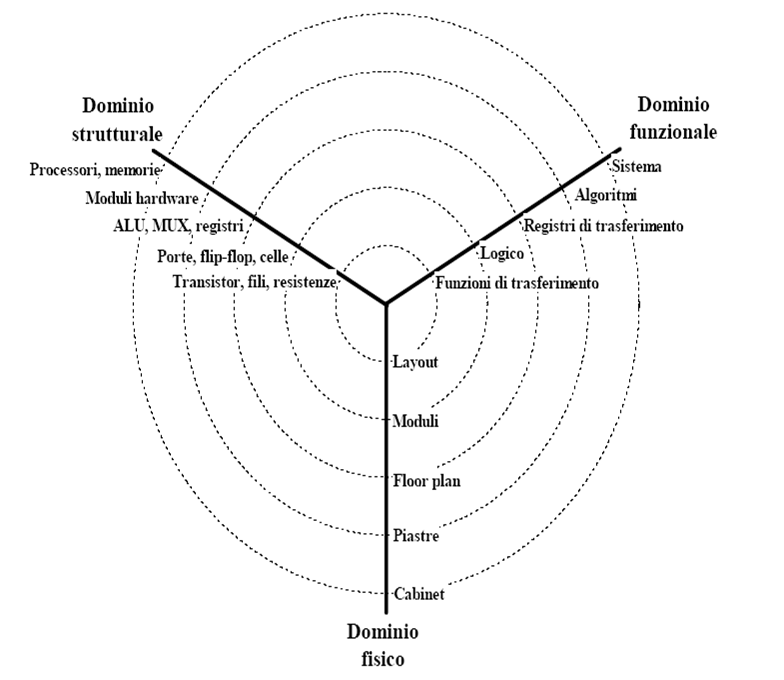
\includegraphics[scale = 0.5]{figures/Ydiag.png}
}{
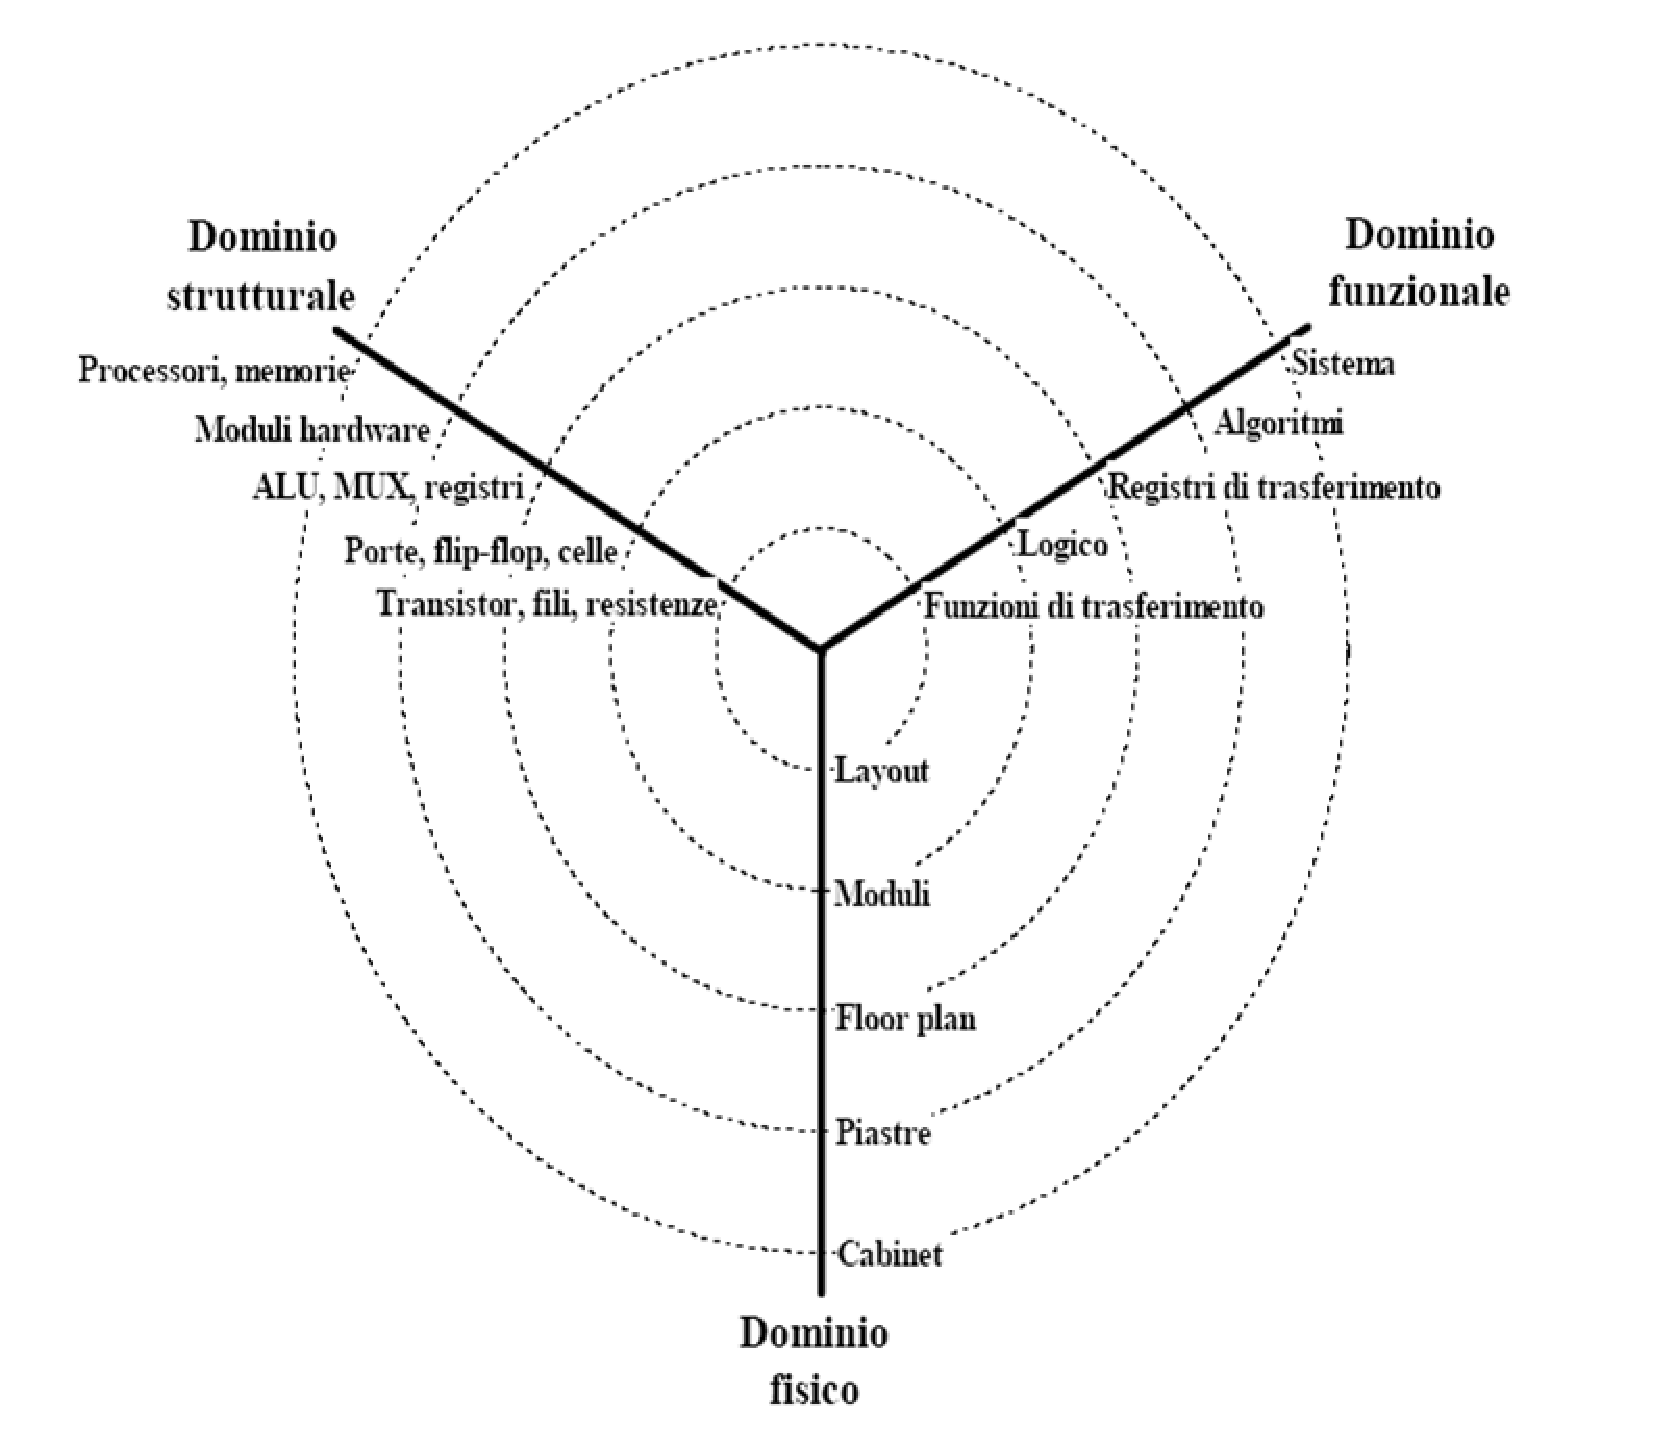
\includegraphics[scale = 0.5]{figures/Ydiag.eps}
}
\ccaption{Livelli di astrazione e domini di rappresentazione}
\label{f:Ydiag}
\end{figure}

Il sistema ed in particolare il circuito che lo implementa possono essere descritti in modalit� diverse. Ogni modalit� � caratterizzata da due aspetti: il dominio di rappresentazione utilizzato (ovvero il particolare punto di vista che si adotta) e il livello di astrazione (ovvero il dettaglio utilizzato nella descrizione stessa). Le possibili modalit� di rappresentazione sono esemplificate dalla figura \ref{f:Ydiag}: gli assi rappresentano i diversi domini di rappresentazione mentre le circonferenze rappresentano i diversi livelli di astrazione, con l'accuratezza che cresce avvicinandosi al centro dei cerchi.

I domini di rappresentazione del circuito (\cite{Ydiag}) sono essenzialmente tre:
\begin{itemize}
\item Funzionale

In questo dominio la descrizione fornisce solo le funzionalit� fornite dal circuito e non la sua struttura; il circuito, o una sua frazione viene rappresentato come una scatola nera di cui vengono forniti solo ingressi, uscite e come queste dipendano dagli ingressi ovvero la funzione che esso implementa. Oltre alla funzionalit� implementata riveste grande importanza in questo tipo di rappresentazioni la descrizione della sua interfaccia cio� le relazioni temporali fra i diversi segnali di ingresso e uscita.

\item Fisico

In questo dominio la descrizione fornisce solo la struttura fisica del circuito ignorando le funzionalit� implementate. Vengono specificate la posizione nello spazio dei diversi componenti e la struttura delle interconnessioni.

\item Strutturale

Le rappresentazioni appartenenti a questo dominio costituiscono un compromesso fra quelle appartenenti agli altri due domini. In genere sono utilizzate nel passaggio fra il primo e il secondo tipo di rappresentazione. Infatti � possibile per il passaggio Funzionale-Strutturale far corrispondere a molti dei componenti della prima rappresentazione dei componenti della seconda e tale corrispondenza � univoca sotto predeterminati vincoli tecnologici. Per passare dalla rappresentazione Strutturale a quella Fisica invece sono in genere necessari due passi: nel primo passo vengono disposti in maniera approssimativa i diversi elementi circuitali curando il posizionamento delle interconnessioni, nel secondo ai componenti circuitali si sostituisce la realizzazione fisica di essi.
\end{itemize}

I livelli di astrazione delle descrizioni, ordinati in modo crescente (cui corrisponde un ordine decrescente di dettaglio) sono invece cinque. Per ciascuno di essi verr� brevemente presentata la descrizione relativa ad ogni dominio di rappresentazione:

\subsubsection{Livello circuito}
\begin{itemize}
\item[] dominio funzionale: la descrizione � realizzata attraverso funzioni di traferimento e diagrammi temporali;
\item[] dominio strutturale: gli elementi base utilizzati nella descrizione sono transistor, resistenze, fili di interconnessione;
\item[] dominio fisico: la rappresentazione utilizzata per la descrizione � quella tipica di un layout di un circuito integrato.
\end{itemize}

\subsubsection{Livello logico}
\begin{itemize}
\item[] dominio funzionale: si utilizzano espressioni booleane;
\item[] dominio strutturale: gli elementi base sono porte logiche, flip-flop e celle;
\item[] dominio fisico: vengono descritti posizionamento di celle e moduli nello spazio.
\end{itemize}

\subsubsection{Livello microarchitetturale o RT}
\begin{itemize}
\item[] dominio funzionale: la descrizione utilizza registri e macchine a stati finiti;
\item[] dominio strutturale: i componenti della descrizione sono le diverse unit� funzionali: unit� aritmetico-logiche, multiplexer, registri, microcontrollori e micromemorie;
\item[] dominio fisico: viene descritto il posizionamento dei componenti elencati nello spazio.
\end{itemize}

\subsubsection{Livello algoritmico-funzionale}
\begin{itemize}
\item[] dominio funzionale: la funzionalit� � descritta attraverso un algoritmo in cui sono definite strutture dati ed operazioni che le devono manipolare; non � necessario che vi sia poi corrispondenza fra struttura dati e componenti architetturali cos� come fra operazioni e unit� funzionali o unit� di controllo; possono essere utilizzati per la descrizione anche linguaggi di descrizione dello hardware;
\item[] dominio strutturale: i componenti di base sono gli stessi del livello microarchitetturale, ma raggruppati in macroblocchi quali linee di trasferimento dati, unit� di controllo e unit� di memorizzazione per sottolineare gli elementi di comunicazione e sincronizzazione fra i diversi componenti;
\item[] dominio fisico: gli elementi utilizzati nella descrizione sono le schede.
\end{itemize}

\subsubsection{Livello sistema}
\begin{itemize}
\item[] dominio funzionale: viene descritta la funzionalit� specificandone i vincoli, in particolare quelli relativi alle prestazioni; si tralascia qualsiasi aspetto implementativo;
\item[] dominio strutturale: gli elementi utilizzati nella descrizione sono processori, memorie, unit� di controllo, switch e bus;
\item[] dominio fisico: viene descritto il posizionamento e la suddivisione del circuito a livello di gruppi di schede o di armadi.
\end{itemize}

\subsection{Linguaggi di specifica del sistema}
I linguaggi di specifica sono linguaggi utilizzati per fornire una descrizione comportamentale del sistema che abbia caratteristiche di formalit�. Tali linguaggi inoltre consentendo un diverso livello di astrazione possono essere utilizzati anche per le rappresentazioni intermedie durante il processo di Sintesi ad Alto Livello. I linguaggi pi� utilizzati sono i linguaggi di descrizione dello hardware (HDL) e SystemC che pu� essere considerato una loro evoluzione.

I linguaggi della descrizione dello hardware sono stati introdotti per favorire lo sviluppo di sistemi hardware permettendo di descrivere con uno stesso linguaggio le caratteristiche del sistema a diversi livelli d'astrazione: funzionale, transazionale, architetturale o logico. E' quindi possibile utilizzare un unico linguaggio come rappresentazione intermedia nelle diverse fasi della Sintesi ad Alto Livello. Inoltre � possibile far convivere nella stessa rappresentazione componenti descritti a livelli di astrazione e quindi di dettaglio diversi. Per questo motivo � possibile raffinare la descrizione solo di alcune parti del sistema mantenendo a grana grossa quella degli altri componenti.

Il primo HDL � stato l'\emph{ISP} formalizzato da Gordon Bell e Alan Newell e descritto in \cite{ISP}. In questo linguaggio veniva per la prima volta introdotta la descrizione a livello RT (register transfert level). Infatti l'ISP era utilizzato per la descrizione del comportamento del computer PDP-8 che veniva modellizzato come un insieme di registri e un insieme di funzioni logiche che descrivevano il trasferimento dati tra di essi.

In seguito nacquero diversi altri linguaggi di descrizione dello hardware: \emph{Vhsic HDL (VHDL)}, \emph{UDLI} sviluppato da NTT, \emph{HiLo}, da cui � stato derivato \emph{Verilog} e \emph{ISP'}, derivato di ISP.

\subsubsection{VHDL}
VHDL � stato sviluppato dal governo degli Stati Uniti d'America, all'interno del programma \emph{``Very High Speed Integrated Circuit (VHSIC)''} iniziato nel 1980.

Questo linguaggio � stato creato con l'intenzione di soddisfare i bisogni che si riscontravano nel processo di progettazione. Le caratteristiche principali di questo linguaggio sono:
\begin{itemize}
\item la possibilit� di rappresentare un sistema come composizione di sottosistemi pi� semplici e di descrivere come questi sottosistemi siano interconnessi fra loro;
\item la possibilit� di rappresentare il funzionamento del sistema utilizzando una forma di linguaggio di programmazione familiare;
\item la possibilit� di simulare il sistema progettato prima che venga effettivamente realizzato e confrontare cos� scelte progettuali diverse;
\item la possibilit� di sintetizzare i circuiti partendo sia dal livello comportamentale che da quello di porta logica.
\end{itemize}

\subsubsection{SystemC}
La crescente domanda di sistemi on chip (SoC) e soprattutto l'aumentare della densit� dei circuiti integrati hanno aperto nuove sfide nella loro progettazione. Infatti la funzionalit� e quindi il sistema implementabile in un singolo circuito integrato � sempre pi� complesso ed � quindi necessario che i progettisti lavorino ad un livello di astrazione maggiore per poter mantenere la produttivit� richiesta. Un altro aspetto che sta influenzando negli ultimi anni la progettazione di sistemi dedicati � la necessit� sempre pi� presente di integrare fortemente le componenti hardware e software del sistema. Sono quindi necessari nuovi approcci per la specifica, il partizionamento e la verifica del sistema. L'utilizzo di linguaggi diversi, linguaggi di specifica Hardware come Verilog o VHDL per la componente HW e linguaggi di programmazione come C o C++ per la componente SW rende comunque difficoltosa questa integrazione.

Una possibile soluzione a questo problema fu individuata in una nuova piattaforma che fosse comune ai due rami di sviluppo di progetto (HW e SW) e che fosse basata su un linguaggio di specifica che consentisse il contemporaneo sviluppo e verifica delle funzionalit� del sistema sia nelle sue componenti Hardware che in quelle Software. La scelta per tale linguaggio � caduta sul C++, opportunamente esteso, perch� solo questo linguaggio poteva garantire un adeguato livello di astrazione, assicurando al contempo una elevata integrazione tra parte hardware e parte software del sistema.

L'estensione proposta ha preso il nome di SystemC: essa � stata sviluppata come un linguaggio standardizzato di specifica e di modellizzazione in grado di poter essere utilizzato per descrizioni a diversi livelli di astrazione e per descrivere sistemi contenenti sia parti hardware che parti software. SystemC � interamente basato su C++, ed il codice relativo al simulatore SystemC � scaricabile gratuitamente da \cite{SystemC} con licenza OCL. Lo standard viene gestito e controllato da un gruppo di tredici componenti in parte di provenienza industriale e in parte accademica.

Fra le caratteristiche peculiari di SystemC si pu� ricordare:
\begin{itemize}
\item permette di descrivere il sistema anche ad un livello di astrazione maggiore rispetto a quello RT;
\item permette di descrivere contemporaneamente componenti Hardware e Software;
\item a livello RT i costrutti di modellazione forniti sono simili a quelli degli altri linguaggi di descrizione dello Hardware;
\item offre costrutti per rappresentare facilmente numeri in virgola fissa;
\item la concorrenza, similmente al VHDL, viene modellata attraverso l'uso di processi;
\item introduce un insieme di funzionalit� per una generica modellazione della comunicazione e della sincronizzazione.
\end{itemize}

I vantaggi offerti da questo linguaggio sono :
\begin{itemize}
\item la validazione del progetto pu� essere realizzata contemporaneamente sia per le componenti hardware che software;
\item il testbench � unico e scritto in un linguaggio basato su C/C++ sia per lo hardware che per il software;
\item le simulazioni possono essere fatte contemporaneamente su software e hardware e potendo essere fatte ad un livello di astrazione superiore all'RT sono generalmente pi� veloci.
\end{itemize}
La caratteristica comune di tutti i vantaggi � quella di poter operare a qualsiasi livello della sintesi di alto livello contemporaneamente su hardware e software.

Ci sono anche degli svantaggi che pi� che tecnologici sono di natura umana; infatti fino all'introduzione del SystemC le progettazioni di componenti HW e SW costituivano due attivit� diverse e abbastanza scorrelate. Pertanto permangono tuttora delle difficolt� nell'integrare questi due ambienti e giungere cos� alla diffusione della figura del progettista HW/SW: i progettisti Hardware hanno scarsa conoscenza del C++, i progettisti software hanno scarsa conoscenza degli strumenti e dei problemi relativi alla progettazione Hardware.

\subsection{Rappresentazioni intermedie}
Le rappresentazioni intermedie sono quelle rappresentazioni utilizzate nelle diverse fasi della Sintesi ad Alto Livello. Ogni fase pu� utilizzare un tipo di rappresentazione diverso per velocizzare la sua computazione, mettere in risalto alcune caratteristiche del sistema o semplificare la scrittura dei risultati intermedi.

La caratteristica che accomuna in generale i tipi di rappresentazione pi� usati � il fatto di essere costituiti da grafi orientati. In particolare i nodi di tali grafi solitamente rappresentano operazioni (o insieme di operazioni come nel caso degli ultimi due tipi di grafo che verranno a breve elencati) mentre gli archi rappresentano delle dipendenze di controllo o di dato fra di esse. Al fine della costruzione di alcune di queste rappresentazioni intermedie, in particolare di quelle che mostrano le dipendenze di controllo, sussiste una grande differenza fra le operazioni rappresentanti costrutti di controllo e operazioni rappresentanti computazioni. Invece, sempre al fine della costruzione dei grafi, distinguere fra i diversi tipi di operazioni computazionali non ha importanza, ma � comunque necessario memorizzarne le caratteristiche all'interno dei grafi stessi affinch� tali informazioni possano essere utilizzate dalle fasi della Sintesi al Alto Livello.

Le rappresentazioni basate su grafi orientati che verranno descritte sono:

\begin{itemize}
\item \emph{Data Flow Graph} (DFG)
\item \emph{Control Flow Graph} (CFG)
\item \emph{Data Dependence Graph} (DDG)
\item \emph{Control Dependence Graph} (CDG)
\item \emph{System Dependence Graph} (SDG)
\item \emph{Control Data Flow Graph} (CDFG)
\item \emph{Grafo dei Blocchi Basici}
\end{itemize}
Fra queste rappresentazioni quelle che verrano utilizzate dall'implementazione dell'algoritmo realizzata sono il System Dependence Graph e il Grafo dei Blocchi Basici insieme ad un'ulteriore rappresentazione basata su grafi non orientati (l'albero dei dominatori) che verr� anch'essa successivamente descritta.

\subsubsection{Data Flow Graph}
Il Data Flow Graph (DFG) � un grafo in cui sono rappresentate le operazioni presenti in un sistema e le dipendenze dati esistenti tra di esse.

Formalmente il DFG � un grafo orientato $G_d(V,E)$ dove:
\begin{itemize}
\item[] $V=\{v_i; i=1,2,...,n_{op}\}$ � l'insieme dei nodi del grafo, dove $n_{op}$ � il numero di operazioni, che si trovano in relazione uno a uno con le singole operazioni del sistema;
\item[] $E=\{(v_i,v_j);i,j=1,2,...,n_{op}\}$ � l'insieme degli archi orientati del grafo: se esiste un arco tra $v_i$ e $v_j$ significa che esiste un trasferimento di dati tra l'i-esima operazione e la j-esima, ovvero che vi � una dipendenza di dato fra le due operazioni.
\end{itemize}

Nel modello DFG non vengono esplicitate le variabili necessarie alla memorizzazione dei dati trasferiti (a differenza del DDG - \ref{c:art:alto:graph:DDG}) fra i diversi nodi del grafo legati da dipendenza. Questo modello pu� inoltre venir utilizzato per la rappresentazione delle dipendenze dato fra sistemi composti da pi� processi per permettere una facile analisi e gestione del flusso di comunicazione fra di essi.

\subsubsection{Control Flow Graph}
Il Control Flow Graph (CFG) � un grafo in cui si rappresentano le operazioni in sequenza cos� come sono ordinate nella specifica evidenziando i possibili branch. Dal punto di vista formale il CFG � un grafo orientato e connesso $G_d(V,E)$ dove:
\begin{itemize}
\item[] $V=\{v_i; i=1,2,...,n_{op}\}$ � l'insieme dei nodi del grafo, dove $n_{op}$ � il numero di operazioni, che si trovano in relazione uno a uno con le singole operazioni del sistema;
\item[] $E=\{(v_i,v_j);i,j=1,2,...,n_{op}\}$ � l'insieme degli archi orientati del grafo: esiste un arco tra $v_i$ e $v_j$ se 
\begin{itemize}
\item la j-esima operazione segue l'i-esima operazione nella specifica del sistema
\item la j-esima operazione � una delle possibili destinazioni dell'i-esma operazione che � di branch, cio� un'operazione che pu� provocare la redirezione del flusso di controllo come cicli, salti, diramzioni, ecc. .
\end{itemize}
\end{itemize}

Questa rappresentazione ha il vantaggio di essere facilmente estraibile dalla specifica iniziale, ma non evidenzia il massimo parallelismo estraibile dal sistema. E' inoltre non adatta a rappresentare sistemi multiprocesso in quanto nel grafo non � immediatamente evidenziabile quali possibili combinazioni fra i diversi percorsi relativi ai diversi processi possono essere contemporaneamente attivi, ne � possibile modellizzare facilmente sincronizzazioni o fork.

\subsubsection{Data Dependence Graph}
\label{c:art:alto:graph:DDG}
Il Data Dependence Graph (DDG) � un grafo che similmente al DFG rappresenta le operazioni presenti in un sistema e le dipendenze dati esistenti tra di esse, ma a differenza del DFG evidenzia anche la variabile che � causa della dipendenza.

Formalmente il DDG � un grafo orientato $G_d(V,E)$ dove:
\begin{itemize}
\item[] $V=\{v_i; i=1,2,...,n_{op}\}$ � l'insieme dei nodi del grafo, dove $n_{op}$ � il numero di operazioni, che si trovano in relazione uno a uno con le singole operazioni del sistema;
\item[] $E=\{(v_i,v_j);i,j=1,2,...,n_{op}\}$ � l'insieme degli archi orientati del grafo: se esiste un arco tra $v_i$ e $v_j$ etichettato $x_k$ devono verificarsi queste condizioni;
\begin{itemize}
\item l'operazione $v_i$ contiene una definizione di $x_k$;
\item l'operazione $v_j$ contiene un uso di $x_k$;
\item esiste un percorso $p$, cio� una possibile traccia di esecuzione, fra le operazioni $v_i$ e $v_j$ le cui operazioni non contengano definizioni di $x_k$.
\end{itemize}
\end{itemize}

\subsubsection{Control Dependence Graph}
Il CDG � un grafo che rappresenta le operazioni presenti in un sistema e le dipendenze di controllo fra di esse. Un'operazione $x_j$ ha una dipendenza di controllo da $x_i$ se $x_i$ � un'operazione di branch e a seconda della direzione del salto intrapreso l'operazione $x_j$ pu� essere eseguita o meno.

Formalmente il CDG � un grafo orientato $G_d(V,E)$ dove:
\begin{itemize}
\item[] $V=\{v_i; i=1,2,...,n_{op}\}$ � l'insieme dei nodi del grafo, dove $n_{op}$ � il numero di operazioni, che si trovano in relazione uno a uno con le singole operazioni del sistema;
\item[] $E=\{(v_i,v_j);i,j=1,2,...,n_{op}\}$ � l'insieme degli archi orientati del grafo: esiste un arco tra $v_i$ e $v_j$ se si verificano entrambe queste condizioni:
\begin{itemize}
\item esiste un percorso $p$ da $v_i$ a $v_j$, tale che $v_j$ post-domina ogni nodo strettamente compreso tra $v_i$ e $v_j$ lungo il percorso $p$;
\item $v_j$ non post-domina il nodo $v_i$.
\end{itemize}
\end{itemize}

La definizione di post-dominanza � la seguente: un nodo $v_i$ post-domina $v_j$ se $v_i$ � diverso da $v_j$ e $v_i$ fa parte di ogni percorso del CFG fra $v_j$ e l'uscita.

\subsubsection{System Dependence Graph} 
La rappresentazione SDG � il risultato della fusione di due rappresentazioni intermedie:  il CDG e il DDG.

Formalmente il SDG � un grafo orientato $G_d(V,E)$ dove:
\begin{itemize}
\item[] $V=\{v_i; i=1,2,...,n_{op}\}$ � l'insieme dei nodi del grafo, dove $n_{op}$ � il numero di operazioni, che si trovano in relazione uno a uno con le singole operazioni del sistema e quindi in corrispondenza uno a uno con i nodi del CDG e i nodi del DDG;
\item[] $E=\{(v_i,v_j);i,j=1,2,...,n_{op}\}$ � l'insieme degli archi orientati del grafo: esiste un arco tra $v_i$ e $v_j$ se si verifica una di queste condizioni:
\begin{itemize}
\item esiste un arco tra $v_i$ e $v_j$ nel CDG;
\item esiste un arco tra $v_i$ e $v_j$ nel DDG.
\end{itemize}
\end{itemize}
Questa rappresentazione � quella pi� utile per gli algoritmi di scheduling perch� permette di considerare contemporaneamente sia le dipendenze dato, sia le dipendenze di controllo e non preordina le operazioni secondo la sequenza in cui si trovano della descrizione della specifica.

\subsubsection{Control Data Flow Graph}
\label{c:art:alto:inter:CDFG}
A differenza delle rappresentazioni precedenti in questo tipo di grafo non vi � una corrispondenza biunivoca con le operazioni della descrizione del sistema.
Le sequenze massime di operazioni che non contengano al loro interno operazioni di salto condizionato ne contengono operazioni destinazione di salti condizionati (ad eccezione della prima operazione della sequenza) vengono raggruppate fra di loro e fatte corrispondere ad un nodo nel grafo. Pi� precisamente si fa corrispondere ad un nodo del CDFG non il mero elenco delle operazioni, ma il DFG parziale che descrive le relazioni di dipendenza dato fra di esse. Le operazioni che non fanno parte di alcune sequenza come per esempio le operazioni di salto condizionato vengono anch'esse fatte corrispondere ad un nodo del grafo.

Formalmente il CDFG � un grafo orientato $G_d(V,E)$ dove:
\begin{itemize}
\item[] $V=\{v_i; i=1,2,...,n\}$ � l'insieme dei nodi del grafo costruito come indicato;
\item[] $E=\{(v_i,v_j);i,j=1,2,...,n_{op}\}$ � l'insieme degli archi orientati del grafo: esiste un arco tra $v_i$ e $v_j$ se 
\begin{itemize}
\item la prima operazione del j-esimo nodo segue una delle operazioni \mbox{dell'i-esimo} nodo nella specifica del sistema;
\item una qualche operazione del j-esimo nodo � una delle possibili destinazioni dell'operazione di salto condizionato corrispondente \mbox{all'i-esimo} nodo.
\end{itemize}
\end{itemize}

Nella sua struttura il CDFG � quindi simile al CFG con la differenza che le catene di operazioni di quest ultimo vengono inserite all'interno di un DFG parziale che costituir� un nodo singolo nel CDFG.

\subsubsection{Grafo dei Blocchi Basici}
Un blocco basico, cos� come definito in \cite{appel}, � una sequenza di operazioni che gode delle seguenti propriet�:
\begin{itemize}
\item la prima operazione � una destinazione di un salto;
\item l'ultima operazione � un salto;
\item non vi sono altre operazioni di salto o destinazione di essi (operazioni etichettate) all'interno della sequenza.
\end{itemize}
Pertanto se un'operazione di un blocco basico viene eseguita in una certa traccia, tutte le operazioni di quel blocco basico verranno eseguite in quella traccia. I blocchi basici di una descrizione di sistema possono a loro volta costituire i nodi di un grafo; tale grafo � molto simile al CDFG ad eccezione che, se un'operazione di salto ha un unico nodo cio� un unico blocco basico come predecessore diretto allora ad esso verr� assegnata e che le operazioni appartenenti ad un unico nodo non vengono descritte da un DFG parziale ma semplicemente elencate all'interno del nodo stesso cos� come compaiono nella specifica.

Formalmente il grafo dei Blocchi Basici � un grafo orientato $G_d(V,E)$ dove:
\begin{itemize}
\item[] $V=\{v_i; i=1,2,...,b\}$ � l'insieme dei nodi che si trovano in relazione uno a uno con i blocchi basici;
\item[] $E=\{(v_i,v_j);i,j=1,2,...,b\}$ � l'insieme degli archi orientati del grafo: esiste un arco tra $v_i$ e $v_j$ se:
\begin{itemize}
\item la prima operazione del j-esimo blocco basico segue l'ultima operazione dell'i-esimo blocco basico;
\item la prima operazione del j-esimo blocco basico � una delle possibili destinazioni del salto con cui termina l'i-esimo blocco basico.
\end{itemize}
\end{itemize}

\subsubsection{Albero dei Dominatori}
A differenza delle precedenti rappresentazioni, l'Albero dei Dominatori come dice il nome stesso non � un grafo orientato bens� un albero ed in particolare costituisce un'elaborazione del grafo dei Blocchi Basici.

Un blocco basico $B_i$ domina un blocco basico $B_j$ se ogni percorso nel grafo dei blocchi basici fra il blocco di ingresso e $B_j$ passa da $B_i$. Un blocco basico pu� avere quindi pi� dominatori. La relazione di dominanza viene estesa includendo le seguenti dominanze:
\begin{itemize}
\item il blocco di ingresso domina tutti i nodi del grafo;
\item ogni blocco domina se stesso.
\end{itemize}

Dalla relazione di dominanza si ricava la relazione di dominanza immediata, pi� utile per analizzare le caratteristiche di un sistema: un blocco basico $B_i$ domina direttamente $B_j$ se:
\begin{itemize}
\item $B_i$ domina $B_j$;
\item non esiste un $B_k$ tali che $B_i$ domina $B_k$ e $B_k$ domina $B_j$.
\end{itemize}

A differenza della relazione di dominanza semplice, ogni blocco basico ha un unico dominatore immediato. A partire dalla dominanza diretta viene costruito l'albero dei dominatori: la radice dell'albero � il blocco basico iniziale; i figli della radice sono i blocchi basici dominati direttamente dal blocco basico iniziale; i figli di un nodo qualsiasi sono i blocchi basici dominati direttamente dal blocco basico corrispondente a quel nodo.

\section{Il problema dello scheduling}
\label{c:art:sch}
Il problema dello scheduling consiste nell'assegnamento delle operazioni che compongono il sistema ad uno specifico passo di controllo, cercando di minimizzare una prefissata funzione obiettivo e rispettando nel contempo un'insieme di vincoli. Funzione obiettivo e vincoli possono riguardare il tempo (numero di passi di controllo o ritardo del sistema) o la tecnologia (numero di unit� funzionali o potenza dissipata).

Nell'ipotesi semplificatrice che tutte le operazioni abbiano tempo di esecuzione uguale (per soddisfare questa ipotesi � sufficiente considerare il tempo di esecuzione di ogni operazione pari al tempo di quella pi� lenta) e posta la durata di un passo di controllo pari a tale tempo, un'operazione pu� essere assegnata solo in un passo di controllo successivo a tutti quelli ai quali sono stati assegnati i suoi predecessori e precedente a quelli nei quali sono stati assegnati i suoi successori.

L'ipotesi appena fatta � tuttavia troppo conservativa e rischia di essere troppo penalizzante nel processo di minimizzazione del tempo di esecuzione della funzionalit�: il tempo di clock ricavato potrebbe risultare infatti troppo lungo. E' quindi necessario considerare la possibilit� che il ritardo introdotto nell'esecuzione delle singole operazioni possa essere diverso. Gli approcci a questa nuova problematica sono sostanzialmente quattro:
\begin{itemize}
\item Multicycling

In questo caso la durata del passo di controllo viene dimensionata sull'operazione pi� veloce; l'esecuzione delle operazioni pi� lunghe richiedr� pi� di un ciclo di controllo (per questo motivo vengono definite operazioni multiciclo). Poich� i dati in ingresso dell'operazione multiciclo potrebbero essere sovrascritti dopo il primo ciclo di clock dall'inizio della sua esecuzione, � necessario introdurre dei latch all'ingresso dell'unit� funzionale che la esegue affinch� i dati vengano tenuti memorizzati. Questo approccio ha tuttavia il difetto di aumentare il numero di passi di controllo richiesti e conseguentemente la complessit� dell'unit� di controllo.

\item Chaining

Il tempo di clock viene mantenuto uguale a quello dell'operazione pi� lenta, tuttavia si consente di eseguire due o pi� operazioni in serie nello stesso passo di controllo. Sostanzialmente si permette di assegnare un'operazione allo stesso ciclo al quale � assegnato l'ultimo dei suoi predecessori purch� la somma dei tempi di esecuzione delle operazioni che costituiscono la serie (operazioni concatenate) sia inferiore al periodo di clock. Tale approccio ha lo svantaggio di richiedere collegamenti diretti fra le diverse unit� funzionali oltre a quelli gi� presenti fra registri ed unit�.

\item Multicycling + Chaining

Il periodo di clock viene posto uguale ad un valore medio dei tempi di esecuzione delle operazioni o al tempo di esecuzione pi� diffuso fra le diverse operazioni. Le operazioni con tempo di esecuzione maggiore del periodo di clock verranno considerate come multiciclo e si permetter� di fare chaining fra quelle con tempo di esecuzione minore della durata di un passo di controllo.

\item Pipeline

Questo approccio � complementare a quelli fin qui presentati e richiede la presenza di unit� funzionali apposite (unit� dotate di pipeline). Le operazioni che possono essere eseguite da questo tipo di unit� sono considerate al pari delle operazioni multiciclo, ma l'unit� funzionale che le esegue viene considerata disponibile a partire dal passo di controllo successivo a quello in cui un'operazione le � stata assegnata.

\end{itemize}


Sommariamente gli algoritmi possono suddividersi in due categorie: quelli che cercano di minimizzare una metrica riguardante le temporizzazioni e quelli che cercano di minimizzare una metrica riguardante la tecnologia.

\subsection{Algortimi che minimizzano metriche temporali}
\label{c:art:sch:time}
All'interno degli algoritmi che hanno come obiettivo quello di minimizzare il tempo di esecuzione (quantit� che pu� essere espressa in modi diversi come per esempio ritardo introdotto dal sistema o numero di passi di controllo) si possono individuare due ulteriori sottocategorie:
\begin{itemize}
\item algoritmi non vincolati: ASAP, ALAP, Path-Based;
\item algoritmi con vincoli sulle risorse: List-Based, Static-List.

Questi algoritmi garantiscono di rispettare i vincoli sulle risorse che si concretizzano in un numero fissato di risorse allocate: a meno della presenza di istruzioni in mutua esclusione introdotta dall'esistenza di costrutti condizionali nel problema, non � possibile schedulare pi� operazioni di un certo tipo rispetto al numero di unit� funzionali allocate che possono eseguire quelle operazioni.
\end{itemize}

\subsubsection{ASAP}
\label{c:art:sch:time:ASAP}
Insieme all'ALAP � uno degli algoritmi pi� semplici: assegna ogni operazione al primo passo di controllo in cui questa pu� essere eseguita rispettando le dipendenze di dato e di controllo presenti nel CDFG. Ogni operazione viene schedulata appena � possibile (\emph{As Soon As Possible}) come descritto in \cite{ASAP1} e \cite{ASAP2}: 
\begin{enumerate}
\item si schedulano tutte le operazioni senza predecessori nel primo passo di controllo;
\item finch� vi sono operazioni ancora da schedulare si ripete:
\begin{enumerate}
\item si incrementa di uno il numero di passi di controllo totale;
\item si schedula nel passo di controllo appena creato una operazione se i suoi predecessori sono gi� tutti stati schedulati in passi di controllo precedenti;
\end{enumerate}
\end{enumerate}
La soluzione trovata � ottima: non esiste uno scheduling possibile che utilizzi un numero di passi di controllo inferiore a quello calcolato dall'ASAP.

\subsubsection{ALAP}
\label{c:art:sch:time:ALAP}
E' il duale dell'ASAP: assegna ogni operazione all'ultimo passo di controllo in cui questa pu� essere eseguita rispettando le dipendenze di dato e di controllo presenti nel CDFG. Ogni operazione viene schedulata il pi� tardi possibile (\emph{As Late As Possible}): 
\begin{enumerate}
\item si schedulano tutte le operazioni senza successori nell'ultimo passo di controllo;
\item finch� vi sono operazioni ancora da schedulare si ripete:
\begin{enumerate}
\item si decrementa di uno l'indice del passo di controllo corrente;
\item si schedula nel passo di controllo corrente una operazione se i suoi successori sono gi� tutti stati schedulati in passi di controllo successivi.
\end{enumerate}
\end{enumerate}
La soluzione trovata � ottima: non esiste uno scheduling possibile che utilizzi un numero di passi di controllo inferiore a quello calcolato dall'ALAP e tale numero coincide ovviamente con quello calcolato dall'ASAP.

Relativamente ad una singola operazione, i passi di controllo compresi fra quello indicato dall'ASAP per quella operazione e quello indicato dall'ALAP prendono il nome di \emph{finestra temporale} dell'operazione; il numero di tali passi di controllo, compresi gli estremi cio� quelli indicati da ASAP e ALAP prende il nome di mobilit� dell'operazione.

\subsubsection{Path--Based}
Il \emph{Path-Based scheduling} (\cite{path1} \cite{path2} e \cite{path3}) minimizza il numero di passi di controllo necessari ad eseguire il percorso critico all'interno del CDFG. Il modo in cui procede l'algoritmo � il seguente: tutti i possibili percorsi di esecuzione sono estratti dal CDFG e sono schedulati indipendentemente l'uno dall'altro. Successivamente lo scheduling dei singoli percorsi viene combinato per generare la soluzione finale.

L'algoritmo genera dei vincoli tra nodi che vengono schedulati in passi di controllo differenti: Il problema di introdurre i vincoli relativi alla minimizzazione dei passi di controllo viene cio� trasformato in un problema di partizionamento di ``clique'' o di sottografi completamente connessi. In questo nuovo problema i nodi rappresentano i vincoli sugli intervalli mentre gli archi rappresentano i vincoli sulla sovrapposizione di intervalli. Una soluzione a questo partizionamento considerer� la minima sovrapposizione di intervalli in un dato percorso. Gli intervalli dei differenti percorsi saranno poi combinati usando la stessa tecnica per ottenere un nuovo CDFG. L'introduzione di nuovi passi di controllo al CDFG finale produrr� infine una unica soluzione finale.

\subsubsection{List Based}
\label{c:art:sch:time:lb}
Come descritto in \cite{lb}, il \emph{List Based scheduling} fornisce una generalizzazione dell'algoritmo ASAP includendo vincoli sul numero delle risorse disponibili. Il funzionamento prevede che ad ogni passo di controllo:
\begin{enumerate}
\item si identifichino i nodi pronti ossia quei nodi i cui predecessori sono gi� stati schedulati;
\item si creino per ogni tipo di unit� funzionale una lista di operazioni pronte che possano da esse essere eseguite; le liste devono essere ordinate in base ad una funzione di priorit�;
\item per ogni lista di operazioni si schedulano le operazioni in ordine di priorit� finche la lista � vuota o finch� non vi sono pi� unit� funzionali di quel tipo disponibili; se vi sono pi� operazioni in lista rispetto al numero di unit� funzionali si differisce lo scheduling di quelle con priorit� minore.
\end{enumerate}

Una possibile funzione di priorit� pu� essere basata sulla mobilit� delle operazioni (differenza fra ALAP e ASAP delle operazioni incrementata di un'unit�): si pu� assegnare una priorit� che � inversamente proporzionale alla mobilit�. In questo modo in uno specifico passo di controllo i nodi con mobilit� pi� bassa saranno quelli che avranno maggiore possibilit� di essere schedulati anticipatamente. Una ridotta mobilit� infatti implica che l'operazione possa essere schedulata in solo pochi passi di controllo. Un'altra possibile funzione di priorit� � l'appartenenza o meno ad uno dei percorsi critici del CDFG.

I risultati dell'algoritmo dipendono fortemente dalla funzione di priorit� scelta. La complessit� temporale e spaziale per questa tipologia di algoritmo � abbastanza elevata, dal momento che � necessario mantenere dinamicamente un elevato numero di liste di priorit�. 

\subsubsection{Static List}
Questo algoritmo (proposto in \cite{static}) � simile al List-Based, ma utilizza un'unica lista di priorit� creata all'inizio dello scheduling che non viene aggiornata dinamicamente. La base per il calcolo della priorit� delle operazioni sono anche in questo caso i risultati forniti da ASAP e ALAP: le operazioni vengono ordinate secondo due chiavi diverse: la prima chiave di ordinamento � il passo di controllo assegnato dall'ALAP; la seconda chiave di ordinamento, che viene utilizzata per operazioni che hanno lo stesso ALAP, � il passo di controllo dell'ASAP. Per entrambe le chiavi si utilizza l'ordinamento decrescente; in caso di nodi con entrambe le chiavi uguali l'ordinamento � arbitrario. Si � cos� ottenuto un assegnamento assoluto di tutte le operazioni. A questo punto sulla base della posizione che le operazioni hanno nella lista si assegna loro una priorit�: i nodi che appartengono all'inizio della lista saranno quelli a minore priorit�, i nodi che appartengono alla coda saranno quelli a maggiore priorit�.

Una volta stabilita la priorit� delle operazioni � possibile eseguire lo scheduling: ad ogni passo di controllo si cerca di schedulare le operazioni a maggiore priorit� purch� esistano unit� funzionali libere capace di eseguirle e vengano rispettate le dipendenze. Qualora un'operazione non possa essere schedulata, il suo scheduling verr� posticipato. A differenza del List Based, la lista non viene aggiornata ad ogni iterazione (proprio da questo deriva l'aggettivo static). Il maggior vantaggio dell'algoritmo consiste proprio nel mancato aggiornamento in quanto in questo modo a differenza del List-Based � necessario costruire una lista di priorit� delle operazioni un'unica volta.

\subsection{Algortimi che minimizzano metriche architetturali}
\label{c:art:sch:func}
Gli algoritmi che hanno come obiettivo quello di minimizzare metriche riguardanti l'architettura (area occupata, potenza dissipata, numero di unit� funzionali) sono caratterizzati dal dover avere il numero di passi di controllo fissato (ci� � fatto implicitamente nel caso del Simulated Annealing); questa caratteristica li rende molto importanti nella progettazione di sistemi real-time caratterizzati soprattutto dalla presenza di  vincoli temporali e dalla necessit� di ridurre aspetti come l'area o la potenza dissipata. Alcuni di questi algoritmi sono stati pensati per minimizzare solo una specifica metrica architetturale (per esempio il numero di unit� funzionali), tuttavia poich� vi � forte dipendenza fra le diverse metriche � facile estenderli per ottenere l'ottimizzazione anche di altre metriche da essa dipendenti. Esistono diversi approcci a questa classe di problemi:
\begin{itemize}
\item Matematico: Programmazione Lineare Intera (ILP);
\item Stocastico: Simulated Annealing;
\item Euristico: Force Directed;
\item Raffinamento Iterativo: Rescheduling Iterativo.
\end{itemize}

\subsubsection{Programmazione Lineare Intera}
Il metodo della Programmazione Lineare Intera (ILP) (\cite{ilp}) trova una soluzione ottima al problema della minimizzazione dei costi delle risorse attraverso una ricerca branch-and-bound che utilizza ``backtracking'' (\ref{c:art:back}).
Siano $S_{Ek}$ e $S_{Lk}$ i passi di controllo a cui � assegnata la k-esima operazione dagli algoritmi ASAP e ALAP. In uno scheduling che rispetti tutte le dipendenze l'operazione k non pu� essere schedulata prima di $S_{Ek}$ e dopo $S_{Lk}$. Da questo, come � gi� stato mostrato, si ricava il valore della finestra temporale di una operazione che per definizione � pari a \[M = \{S_{j} | E_k \leq j \leq L_k\},\] Dalla finestra temporale di un'operazione 	si ricava facilmente  la sua mobilit� che � il numero di passi di controllo compresi tra $S_{Ek}$ e $S_{Lk}$ estremi inclusi.
La notazione usata per questo tipo di formulazione prevede l'introduzione e la definizione delle seguenti quantit�:
\begin{description}
\item[$OP=\{O_i | 1 \leq i \leq n\}$] insieme delle operazioni;
\item[$t_i=$] tipo dell'i-esima operazione;
\item[$T=\{t_k | 1 \leq k \leq m\}$] insieme dei possibili tipi;
\item[$OP_{tk}$] operazioni in OP di tipo $t_k$;
\item[$INDEX_{tk}$] insieme degli indici di operazioni in $OP_{tk}$;
\item[$N_{tk}$] numero di unit� che compiono operazioni di tipo $t_k$;
\item[$C_{tk}$] costo di tali unit�;
\item[$S=\{s_j | 1 \leq j \leq r\}$] insieme di passi di controllo disponibili per lo scheduling delle operazioni;
\item[$x_{ij}$] variabili logiche che indicano l'assegnamento di un'operazione $i$ ad un passo di controllo $j$: 1 in caso di assegnamento, 0 in caso contrario
 \end{description}
Il problema dello scheduling pu� quindi essere formulato come:
\[minimizza (\Sigma_{k=1}^{m}(C_{tk} * N_{tk}))\]
con i vincoli:
\begin{itemize}
\item un'operazione pu� essere schedulata in un unico passo di controllo e questo passo di controllo deve far parte della sua finestra temporale

\[\forall i, 1 \leq i \leq n, (\Sigma_{E_j \leq j \leq L_j} x_{ij}=1);\]

\item il numero di operazioni di tipo $t_k$ schedulate in un passo di controllo non pu� essere maggiore del numero di unit� funzionali che possono eseguire operazioni di tipo $t_k$ (nel caso non esistano operazioni in mutua esclusione a causa della presenza di costrutti di controllo)

\[\forall j, 1 \leq j \leq r, \forall k, 1 \leq k \leq m, (\Sigma_{j \in INDEX_{tk}} x_{ij} \leq N_{tk});\]

\item un'operazione non pu� essere schedulata prima dei successori

\[\forall i,j,o_i \in Pred_{o_j}(\Sigma_{E_i \leq k \leq L_i}(k \cdot x_{ik})- \Sigma_{E_j \leq l \leq L_j}(l \cdot x_{jl})\leq -1).\]
\end{itemize}
L'algoritmo ha complessit� elevata e quindi il tempo di esecuzione cresce molto rapidamente al crescere del numero di variabili utilizzate. Non � quindi utilizzabile direttamente in casi che non siano molto semplici: ne sono state pertanto realizzate versioni modificate che non fanno uso di backtracking, ma utilizzando tecniche euristiche assegnano un'operazione alla volta invece di tentare di trovare una soluzione completa.

\subsubsection{Simulated Annealing}
L'algoritmo \emph{Simulated Annealing} � descritto in \cite{path1}. Il problema dello scheduling in questo caso viene rappresentato attraverso una tabella in cui le righe raffigurano i passi di controllo, mentre le colonne rappresentano le unit� funzionali disponibili: il problema � quindi quello di posizionare le operazioni all'interno di questa tabella, imponendo il vincolo legato al fatto che in un passo di controllo una risorsa pu� essere utilizzata per un'unica operazione. Ogni cella conterr� quindi una sola operazione (considerando solo problemi senza costrutti condizionali).

L'algoritmo parte da una soluzione iniziale che deve essere precalcolata e per successive iterazioni effettua delle modifiche allo scheduling iniziale. Ad ogni iterazione viene valutata la bont� di questa modifica, che pu� essere accettata con una certa probabilit� dipendente dal guadagno ottenuto relativamente alla funzione obiettivo. La funzione obiettivo tipicamente riguarda aspetti architetturali del sistema. Anche in caso di peggioramento delle prestazioni o della funzione obiettivo � possibile, seppur ovviamente con probabilit� minore, che la nuova soluzione venga accettata. L'accettare anche soluzioni peggiorative permette di uscire dai minimi locali della funzione obiettivo garantendo in tal modo una pi� esaustiva esplorazione dello spazio delle soluzioni.

Per tale motivo questo algoritmo pu� essere considerato particolarmente robusto, anche se tale robustezza si ripercuote in termini di tempi di esecuzione.

\subsubsection{Force Directed}
Il \emph{Force Directed} scheduling (\cite{fd1} e \cite{fd2}) � l'algoritmo di cui si propone un'estensione in questo lavoro di tesi, quindi verr� descritto accuratamente nel capitolo \ref{c:ori}. Se ne d� qui per completezza del confronto con gli altri algoritmi presentati una breve descrizione.

Il Force Directed � un metodo euristico con l'obiettivo di minimizzare il numero totale di unit� funzionali utilizzate fissato il numero di passi di controllo. Per minimizzre questo valore l'algoritmo cerca di distribuire uniformemente le operazioni di uno stesso tipo nei diversi passi di controllo. Come gli  algoritmi precedenti necessita delle informazioni fornite da ASAP e ALAP.

La soluzione dell'algoritmo non � ottima a causa di alcune approssimazioni che vengono fatte durante la sua esecuzione sugli effetti prodotti dai singoli assegnamenti.

\subsubsection{Rescheduling Iterativo}
Il metodo del \emph{Rescheduling Iterativo (IR)} (\cite{iter}) si basa sul problema della bisezione di grafi (proposto da Kernighan e Lin in \cite{part}) e procede similmente al Simulated Annealing reschedulando singolarmente le operazioni e  necessita quindi di una soluzione ammissibile gi� esistente. Tale soluzione viene modificata in questo modo: si sceglie un'operazione casualmente, la si sposta in un altro passo di controllo e la si blocca; si ripete ci� finch� tutte le operazioni sono bloccate. Dopo ogni modifica si valuta il guadagno che questa comporta: la sequenza di spostamenti che produce il miglior guadagno viene effettivamente applicata allo scheduling ottenendo una nuova soluzione. A partire da questa soluzione si riapplica una nuova iterazione dell'algoritmo finch� non si giunge ad una soluzione accettabile.

La bont� dei risultati dipende fortemente dalla soluzione iniziale utilizzata; esistono delle varianti che si possono introdurre per ovviare a questa limitazione rendendo meno critica la scelta della soluzione iniziale e migliorando la qualit� media dei risultati; i miglioramenti che possono essere apportati sono:
\begin{itemize}
\item utilizzare diverse configurazioni iniziali: l'algoritmo � computazionalmente efficiente e quindi pu� essere applicato pi� volte;
\item utilizzare una migliore strategia di previsione degli effetti.
\end{itemize}

\section{La tecnica del Backtracking}
\label{c:art:back}
Il \emph{Backtracking} � una tecnica di tipo costruttivo utilizzata nel risolvere problemi caratterizzati dall'esistenza di vincoli da soddisfare. Il termine \emph{backtrack} fu coniato dal matematico americano D. H. Lehmer nel  1950, ma la prima generale esposizione di questa tecnica � dovuta a Walker (\cite{back1}) e fra i primi studi generali si possono ricordare \cite{back2} e \cite{back3}. I problemi che questa tecnica pu� risolvere sono modellizzabili solitamente come la scelta di quale valore assegnare ad una serie di variabili. Una possibile rappresentazione di questo modello sono gli alberi di ricerca: ai nodi intermedi corrispondono soluzioni intermedie, alle foglie le soluzioni complete, agli archi le possibili scelte di assegnamento di una variabile e quindi i passi che contribuiscono a costruire la soluzione finale.

La ricerca della soluzione pu� essere modellizzata come una visita \mbox{deptu-first} dell'albero di ricerca (una volta giunti in un nodo la visita procedeh nel primo dei suoi figli; solo nel caso tutti i figli di un nodo siano gi� stati visitati si passa alla visita dei suoi fratelli). Per ottenere la soluzione ottima, cio� la soluzione in cui il valore di una certa funzione obiettivo � minimo, � necessario esplorare l'intero albero.

La tecnica appena descritta impone quindi di analizzare tutte le soluzioni possibili per individuare quella ottima. Per limitare il numero di soluzioni da esaminare � possibile utilizzare il metodo del \emph{Branch and Bound}; questo consiste nel calcolare il soddisfacimento dei vincoli e il valore della funzione obiettivo non solo per le foglie, ma per tutti i nodi dell'albero e tagliare i sottoalberi che offrono soluzioni sicuramente peggiori di quella trovata fino a quel momento.  Si supponga per esempio che i contributi dei singoli assegnamenti alla funzione obiettivo siano tutti non negativi: se in un nodo il valore della funzione obiettivo � pi� grande di quello della miglior soluzione trovata, tutte quelle corrispondenti alle foglie appartenenti al sottoalbero avente origine in quel nodo avranno un valore della funzione obiettivo peggiore della soluzione temporanea e pertanto potranno essere ignorate, riducendo quindi il numero di soluzioni da considerare.

Il backtracking ha complessit� esponenziale quindi � poco efficiente per risolvere problemi che non siano NP-completi; � possibile tuttavia integrare al suo interno euristiche, come quella appena presentata del Branch and Bound, che, pur non riducendo la complessit� del caso pessimo, possono ridurre il tempo di esecuzione medio.

\subsection{Tecniche di Look-Ahead}
\label{c:art:back:la}
Le tecniche di Look-Ahead sono tecniche che estendono ed integrano quella del Backtracking consentendo di ridurre il numero di nodi da visitare dell'albero sia nel caso l'obiettivo sia individuare una soluzione valida, sia nel caso si voglia trovare una soluzione il cui valore della funzione obiettivo sia soddisfacente. Nella versione classica del Backtracking la scelta del prossimo arco e quindi del prossimo assegnamento a partire da un certo nodo � casuale o determinata dall'ordinamento lessicografico degli assegnamenti stessi.

L'idea alla base del Look-Ahead � quella di stimare gli effetti dovuti al prossimo assegnamento prima di scegliere quale arco percorrere. In questo modo � possibile escludere assegnamenti che provocherebbero una violazione dei vincoli del problema e cercare di percorrere anticipatamente il ramo che porta ad una soluzione se non ottima almeno accettabile secondo dei criteri prefissati.

E' possibile estendere l'orizzonte visivo di questa tecnica a pi� passi cio� cercare di stimare la qualit� delle soluzioni parziali costruite a partire da quella attuale aggiungendo non uno ma pi� assegnamenti. Il risultato � di ridurre il numero medio di backtracking necessari (nel caso si voglia individuare una soluzione ammissibile) oppure di ottenere una soluzione mediamente migliore (nel caso si stia cercando di minimizzare una certa metrica senza comunque voler ottenere la soluzione ottima) a prezzo di una crescita del tempo di computazione medio dovuta all'overhead necessario per calcolare le stime delle soluzioni parziali.
\chapter{Il Force Directed Scheduling proposto da Paulin e Knight}
\label{c:ori}
\thispagestyle{empty}

\vspace{0.5cm}

L'algoritmo del Force Directed scheduling fu presentato per la prima volta da Paulin e Knight in \cite{fd1} come nuovo componente del sistema ad approccio multiplo per la sintesi automatica denominato \emph{HAL} (\cite{hal}) e successivamente esteso in \cite{fd2}. Nella sua formulazione base il Force Directed � un algoritmo di scheduling a tempo vincolato (i vincoli temporali possono essere requisiti di progetto oppure essere calcolati tramite altri algoritmi come ASAP (\ref{c:art:sch:time:ASAP}), ALAP (\ref{c:art:sch:time:ALAP}) o List-Based (\ref{c:art:sch:time:lb})) che mira a minimizzare il numero di unit� funzionali, bus e registri richiesti per implementare una certa funzionalit� tramite il bilanciamento in ogni passo di controllo del numero di operazioni assegnate ad un certo tipo di risorsa. Il bilanciamento della distribuzione delle operazioni induce ovviamente l'uniformarsi dell'utilizzo delle unit� funzionali nei diversi passi di controllo e conseguentemente riduce il picco massimo di richieste di un certo tipo di risorsa. Tale numero corrisponder� al numero di unit� funzionali di quel tipo che sar� necessario allocare per implementare la funzionalit�. L'algoritmo � iterativo e costruttivo: ad ogni iterazione un'operazione, sulla base delle procedure che verranno esposte in \ref{c:ori:core}, verr� assegnata ad un passo di controllo.

Nella prima sezione verr� illustrata la prima versione dell'algoritmo che prevede la semplificazione che tutte le operazioni vengano eseguite in un tempo uguale e fissato che verr� identificato come durata del passo di controllo.

Nella seconda sezione verr� invece mostrato come � possibile superare queste limitazioni e come introdurre informazioni relative alla tecnologia target all'interno dell'algoritmo.

\section{L'algoritmo nella sua versione base}
\label{c:ori:core}
L'algoritmo del Force Directed scheduling si fonda sul concetto di forza da cui prende il nome. Ad ogni coppia <operazione-passo di controllo> viene associata una forza cio� un numero reale indice dell'effetto del scegliere quel particolare assegnamento <operazione-passo di controllo> sulla uniformit� della distribuzione delle operazioni di qualsiasi tipo non solo in quel passo di controllo, ma in tutti i passi di controllo influenzati. Un valore positivo indica un aumento delle operazioni concorrenti per le stesse risorse e quindi un peggioramento della situazione rispetto a quella desiderata, un valore negativo invece indica una diminuzione della concorrenza e quindi un possibile ridursi delle unit� funzionali richieste.

Il metodo per calcolare questo valore prende spunto dalla legge di Hooke per i corpi elastici (molle): \begin{equation}
F = -kx
\end{equation}
dove:
\begin{description}
\item[F] � la forza esercitata dalla molla che si oppone all'allungamento;
\item[k] � la costante di Hooke;
\item[x] � la distanza della quale viene allungata la molla.
\end{description}

\begin{figure}
\begin{center}

\ifthenelse{\boolean{pdf}}
{
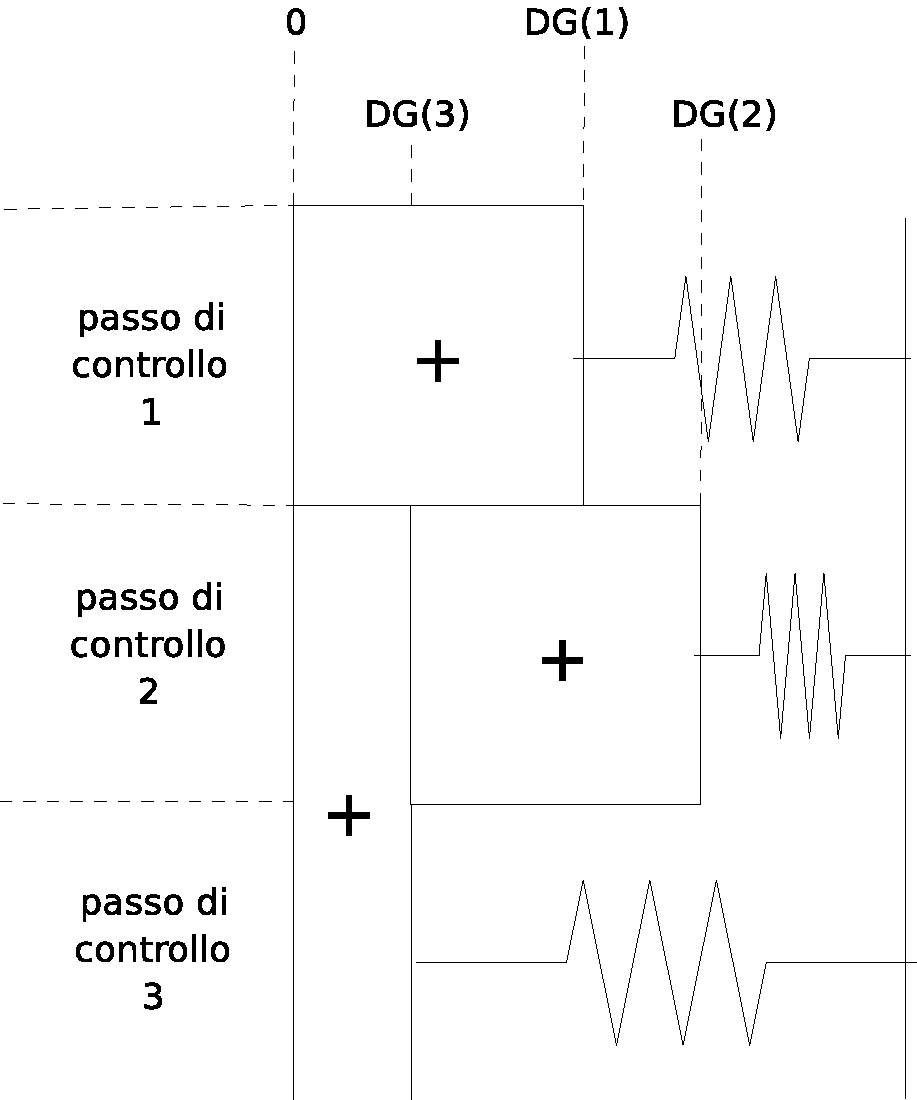
\includegraphics[scale = 0.40]{figures/Diagram15.pdf}
}{
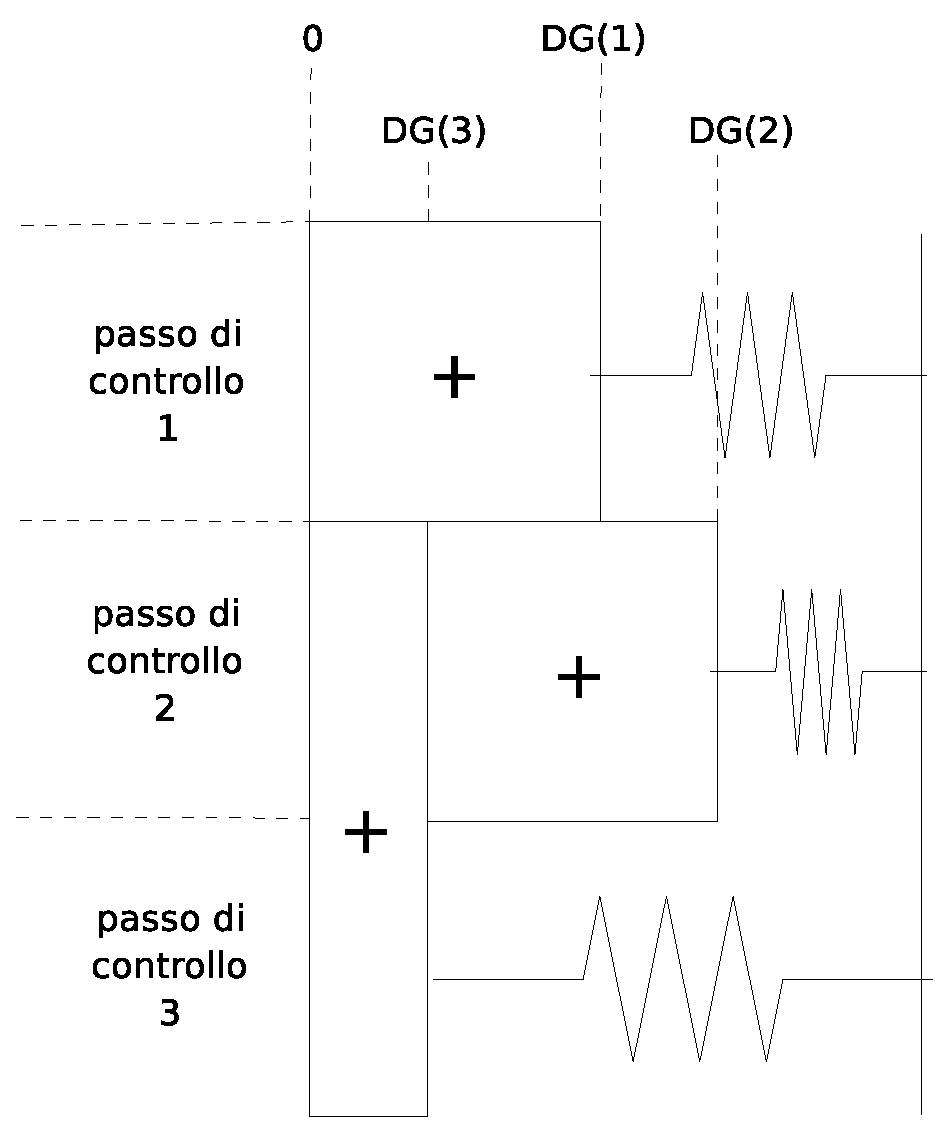
\includegraphics[scale = 0.40]{figures/Diagram15.eps}
}
\hcaption[Esempio di interpretazione dell'algoritmo del Force Directed scheduling]{Esempio di interpretazione dell'algoritmo del Force Directed scheduling: i due quadrati ed il rettangolo contenenti il simbolo della somma rappresentano delle operazioni e la loro probabilit� che siano assegnate ad un passo di controllo (maggiore � l'area, maggiore � la probabilit�). La distanza fra 0 e DG(i) rappresenta la somma di probabilit� per l'i-esimo passo di controllo: si ipotizza che le molle rappresentate nella parte destra abbiano costante di elasticit� pari alle somme di probabilit� dei rispettivi passi di controllo. Si ipotizza inoltre che tali molle si trovino in stato di compressione. Simbolicamente quindi le molle premono contro le operazioni cercando di uniformare il livello delle somme di probabilit� per giungere ad uno stato stabile del sistema in cui le forze esercitate dalle singole molle siano uguali. Infatti la forza esercitata da una molla � tanto maggiore quanto maggiore � la somma di probabilit� perch� maggiore � la sua costante elastica e la sua compressione. C'� da sottolineare tuttavia come a differenza di quelle reali, le molle utilizzate in questo esempio abbiano costante elastica variabile.}
\label{f:molla}
\end{center}
\end{figure}


L'idea � che venga assimilata ad una molla la somma delle probabilit� delle operazioni relativa ad una coppia <passo di controllo-tipo di unit� funzionale> cio� un numero non necessariamente intero che indichi il numero di operazioni di quel tipo che "probabilmente" verranno associate a quel passo di controllo (per rispettare i segni delle equazioni � pi� corretto dire che alla molla corrisponde il complemento rispetto ad un'ipotetica costante della somma di probabilit�; come calcolare le funzioni di distribuzione della probabilit� delle operazioni che sono necessarie per calcolare la somma e come ottenere la somma stessa verr� illustrato in \ref{c:ori:core:prob}. Questa quantit�, proseguendo nell'analogia con i corpi elastici (confrontare figura \ref{f:molla}), esercita una forza nei confronti delle operazioni stesse che contribuiscono a formarla: la scelta di un assegnamento di un'operazione ad un passo di controllo comporter� la sua eliminazione da tutti i passi di controllo (con conseguente "allungamento" della molla e quindi insorgere di una forza negativa) tranne quello scelto in cui la somma di probabilit� aumenter� (equivalentemente ad una "compressione della molla" e quindi ad una forza positiva). Sommando le forze dovute alle variazioni nei diversi passi di controllo si otterr� quindi un indice complessivo della variazione della concorrenza delle operazioni nel sistema. Una forza complessivamente negativa corrisponder� ad un allungamento medio delle molle e quindi alla diminuzione media delle somme di probabilit� e quindi del numero medio di risorse necessarie nei diversi passi di controllo.

\subsection{Calcolo delle somme di probabilit�}
\label{c:ori:core:prob}
Alla base del calcolo delle somme di probabilit� c'� la necessit� di conoscere la distribuzione di probabilit� nei vari passi di controllo relativa ad ogni operazione. Per ottenerle si consideri innanzitutto che non tutte le operazioni sono schedulabili in tutti i passi di controllo. Le dipendenze di dato e le dipendenze di controllo impongono che alcune operazioni possano venir eseguite solo a condizione che quelle da cui esse dipendono siano concluse (a meno di considerare ipotesi speculative). Nei passi di controllo in cui � impossibile assegnare un'operazione non esistendo alcuno scheduling comprendente quell'assegnamento che possa soddisfare tutti i vincoli di dipendenza poniamo pari a zero la probabilit� che quella operazione vi venga schedulata. Poich� a priori non disponiamo di alcuna altra informazione sulle probabilit� nei diversi passi di controllo � bene utilizzare come distribuzione di probabilit� quella che statisticamente minimizza l'errore di approssimazione nel caso di nessuna informazione: la distribuzione uniforme. Detto mobilit� il numero di passi di controllo in cui � possibile schedulare un'operazione, alla sua probabilit� di venir assegnata in uno particolare di questi passi verr� attribuito il valore di $\frac{1}{mobilita'}$.

Rimane il problema di individuare in quali passi di controllo � possibile schedulare una certa operazione (denominati finestra temporale di un'operazione) e quindi la mobilit�. La soluzione a ci� � offerta dagli algoritmi ASAP e ALAP: il primo fornisce infatti il primo passo di controllo in cui una certa operazione pu� essere schedulata, il secondo fornisce l'ultimo passo. Inoltre questi algoritmi calcolano in modo ottimale il numero di passi di controllo minimo necessario per eseguire tutte le operazioni rispettando i vincoli di dipendenza. Questo valore � anche quello che assume per il suo calcolo l'algoritmo del Force Directed scheduling base.

Una volta ottenuta le probabilit� che le singole operazioni possano essere schedulate in un certo passo di controllo � necessario ricavare la somma di questi valori. Queste somme danno un indice del numero di unit� funzionali che in quel dato di controllo probabilmente saranno utilizzate. Al di l� dell'aspetto intuitivo di questa corrispondenza, viene qui presentata una giustificazione matematica non presente in \cite{fd1} e \cite{fd2}. Considerato un passo di controllo fissato e un tipo di operazione fissato, per ognuna delle operazioni di quel tipo schedulabili in quel passo di controllo viene creata una variabile aleatoria discreta $X_i$ che pu� assumere valore $0$ (l'operazione non viene schedulata in quel passo di controllo) o $1$ (l'operazione viene assegnata a quel passo di controllo). Tale variabile casuale sar� evidentemente una Bernoulliana di parametro pari alla probabilit� che tale operazione venga schedulata in quel passo. Al fine dei calcoli si pu� ipotizzare che le variabili siano tutte indipendenti (semplificazione insita nell'algoritmo stesso, ma non corrispondente alla realt� in quanto le probabilit� che un'operazione venga schedulata in un certo passo dipende s� solo dalla sua mobilit�, ma potrebbero esistere dipendenze fra le mobilit� delle operazioni schedulabili contemporaneamente: per esempio un'operazione potrebbe dipendere dall'altra). Si consideri infine un'ulteriore variabile aleatoria $Z$ che modellizzi il numero di operazioni del tipo fissato schedulate in quel passo di controllo. Si avr� quindi (nel caso di assenza di costrutti condizionali):
\begin{equation}
Z = \sum_i X_i
\end{equation}
con gli $X_i$ che possono assumere valore 0 o 1. La media di questa variabile sar�
\begin{align*}
\mathds{E} [Z] & = \mathds{E}[\sum_i X_i] \\
\intertext{essendo le variabili indipendenti si pu� invertire l'operatore $\sum$ con $\mathds{E}$}
\mathds{E}[Z] & = \sum_i \mathds{E}[X_i] \\
\intertext{ma $\mathds{E}[X_i] = p _i$ dove $p_i$ � il parametro della bernouliana cio� la probabilit� dell'operazione}
\mathds{E}[Z] & = \sum_i p_i = DG(c)
\end{align*}
Con DG(c) si indica la somma di probabilit� nel passo \emph{c} delle operazioni del tipo fissato.

In questo modo � stata dimostrata la stretta corrispondenza fra le somme di probabilit� e l'utilizzo di un determinato tipo di unit� funzionale. La somma di probabilit� non pu� limitarsi per� ad una mera somma algebrica proprio perch� il risultato finale dovr� essere un indice di quante unit� funzionali di un certo tipo verranno probabilmente utilizzate in un determinato passo di controllo. Nel caso la funzionalit� originaria che si voglia schedulare presenti al suo interno dei costrutti di controllo (come ad esempio degli IF, WHILE, etc.) � non solo possibile ma probabile che esistano una o pi� coppie (o combinazioni di numero maggiore) di operazioni in mutua esclusione reciproca, tali cio� che solo una di esse debba essere eseguita all'interno di una singola traccia di esecuzione della funzionalit�. Pertanto � impossibile che esse richiedano simultaneamente l'utilizzo di una particolare unit� funzionale, quindi per calcolare il numero di unit� funzionali probabilmente occupate non � significativo sommare le probabilit� delle singole operazioni, ma � necessario tenere in considerazione queste possibilit�. Una prima approssimazione suggerirebbe di utilizzare la media delle probabilit� delle operazioni in mutua esclusione, ma poich� lo scopo finale dell'algoritmo � comunque quello di minimizzare il massimo utilizzo di una certa unit� funzionale, viene preso in esame il valore massimo fra di esse. Queste considerazioni relative a singole operazioni si estendono immediatamente in caso di situazioni pi� complesse con presenza di basic block in mutua esclusione. In questo caso si calcola la somma di probabilit� relativa ai singoli blocchi basici sommando le probabilit� delle operazioni appartenenti ad essi come se il blocco basico rappresentasse una macro-operazione ottenuta fondendo le singole operazioni. Tale macro-operazione potr� avere probabilit� anche maggiore di uno potendo occupare pi� unit� funzionali poich� � il risultato della fusione di diverse operazioni elementari. Una volta eliminati ai fini del calcolo i blocchi basici dominati a livello di probabilit� da blocchi basici con probabilit� totale maggiore � possibile ottenere il valore finale desiderato sommando le probabilit� delle operazioni rimaste. Gruppi di operazioni appartenenti a rami di costrutti condizionali, ma che non siano in mutua esclusione con alcuna altra operazione dello stesso tipo vanno considerati al fine del calcolo come eseguite in ogni traccia di esecuzione.

\subsection{Calcolo delle Forze}
\label{c:ori:core:force}
Una volta calcolate le somme delle probabilit� � possibile calcolare le forze che stanno alla base dell'algoritmo di scheduling. Si calcola una forza per ogni coppia <operazione-passo di controllo possibile> (gli scheduling possibili come � stato evidenziato sono quelli calcolati dagli algoritmi ASAP - ALAP). Il valore di ogni forza si calcola sommando due diversi contributi, il primo detto \mbox{\emph{self-force}} (autoforza) che si riferisce agli effetti dello scheduling dell'operazione in oggetto, il secondo detto \emph{predecessors' and successors' force} (forza di predecessori e successori) che tiene conto della restrizione della finestre temporali dei predecessori (predecessori nel SDG cio� quelle operazioni da cui quella considerata dipende) e dei successori (successori nel SDG cio� quelle operazioni che dipendono da quella considerata) dell'operazione esaminata. Infatti uno scheduling equivale a restringere ad uno la mobilit� di un'operazione, riduzione che pu� causare la restrizione della mobilit� di altre operazioni. Un assegnamento quindi pu� causare non solo la modifica delle somme di probabilit� relative all'unit� funzionale che esegue quella operazione e relative a quei passi di controllo interessati dall'operazione, ma anche di altri passi di controllo e di altre unit� funzionali. Come gi� anticipato la funzione utilizzata per calcolare le forze ricalca la legge di Hooke:
\begin{equation}
Force(i) = DG(i) \cdot x(i)
\end{equation}
dove 
\begin{description}
\item[Force(i)] � il contributo alla forza dello scheduling relativo all'i-esimo passo di controllo;
\item[DG(i)] � la somma di probabilit� del tipo di unit� funzionale che pu� eseguire l'operazione nell'i-esimo passo di controllo;
\item[x(i)] � la variazione della probabilit� dell'operazione nell'i-esimo passo di controllo a seguito dello scheduling.
\end{description}

Questa formula permette di calcolare il contributo alla forza relativo ad un passo di controllo dell'assegnamento. La \emph{self-force} complessiva � pari alla somma dei contributi relativi ai singoli passi di controllo. Ovviamente tali contribuiti saranno pari a zero per i passi di controllo nei quali non � possibile schedulare l'operazione perch� il terzo termine della formula sar� nullo. La variazione della probabilit� dell'operazione � facilmente calcolabile in $-\frac{1}{mobilita'}$ per tutti i passi di controllo dove l'istruzione era schedulabile ad eccezione di quello dell'assegnamento che sar� pari a $+\frac{mobilita'-1}{mobilita'}$. Una possibile diversa interpretazione del terzo termine della formula e quindi del calcolo della forza verr� illustrata in \ref{c:my:var:force}. La \emph{self-force} complessiva sar� positiva nel caso il passo di controllo dell'assegnamento abbia somma di probabilit� mediamente superiore alle altre, negativa in caso contrario.

Allo stesso modo � possibile calcolare la \emph{predecessors' and successors' force}: per ogni predecessore e successore la cui mobilit� � modificata dal possibile scheduling si applica la formula utilizzata per il calcolo della \emph{self-force} tenendo in considerazione le variazioni delle probabilit� delle operazioni dovute alla restrizione della mobilit�. A differenza del caso del calcolo della \emph{self-force} la nuova mobilit� di un'operazione pu� essere maggiore di uno, quindi la formula per la modifica della probabilit� illustrata precedentemente pu� non valere. Le singole forze cos� ottenute vengono sommate per dare origine alla \emph{predecessors' and successors' force}. Va sottolineato come il calcolo delle forze di predecessori e successori avvenga singolarmente e non considerando complessivamente gli effetti della restrizione della mobilit� di istruzioni contemporanee. Facendo riferimento all'analogia con la fisica descritta in \ref{c:ori:core} � come se si considerasse valido nel problema del calcolo delle forze il principio di sovrapposizione degli effetti. In realt� questa � solo una semplificazione introdotta dall'algoritmo perch� non corrisponde alla situazione reale del problema. Infatti bisognerebbe considerare che, dato lo scheduling di un'operazione avente pi� predecessori che subiscono una restrizione della mobilit� a seguito dell'assegnamento stesso, si pu� notare nell'esempio riportato nella figura \ref{f:ex} come per calcolare la forza relativa a ciascun predecessore sarebbe pi� corretto considerare l'effetto causato dalla restrizione della mobilit� degli altri predecessori a lui contemporanei in quanto questa restrizione modifica la somma di probabilit� e quindi anche la forza. Infatti se si analizza la tabella riportata in \ref{f:ex:tab} riferendosi in particolare alle forze dell'operazione \emph{-5} si pu� notare come la forza relativa allo scheduling nel passo di controllo 1 sia nettamente negativa. Infatti questo scheduling, la cui \emph{self-force} � 0 perch� i due passi in cui � possibile schedulare l'operazione hanno la stessa somma di probabilit�, comporta la riduzione del frame delle operazione \emph{+2}, \emph{+3} e \emph{+4} da [0 1] a [0 0] con un contributo di forza negativo poich� la somma di probabilit� iniziale relativa all'operazione di somma nel passo 1 � superiore a quella del passo 0. Apparentemente quindi lo scheduling spinge queste tre operazioni in un passo di controllo mediamente meno congestionato come ci si aspetta che faccia l'algoritmo. Tuttavia � facile notare che lo scheduling contemporaneo delle tre istruzioni al primo passo di controllo non costituisce la soluzione ottimale al problema di scheduling presentato. Confrontando lo scheduling ottenuto dall'applicazione dell'algoritmo in \ref{f:ex:fd} con quello costruito manualmente in \ref{f:ex:hand} si pu� notare come la soluzione ottimale utilizzi due sommatori contro i tre calcolati dal Force Directed. Un possibile modo per ovviare a questa limitazione della formulazione originaria dell'algoritmo verr� presentato in \ref{c:my:var:corr}.

\begin{figure}
\begin{center}
\subfigure[DFG di esempio]{
\fbox{
\ifthenelse{\boolean{pdf}}
{
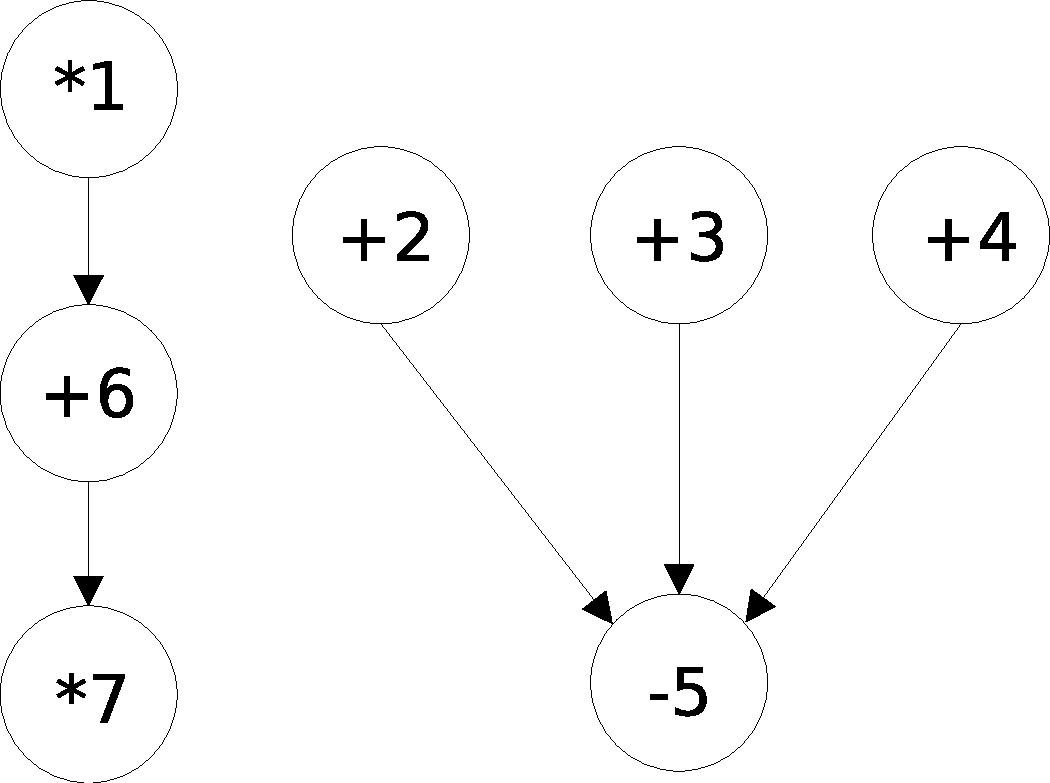
\includegraphics[scale = 0.22]{figures/Diagram1.pdf}
}{
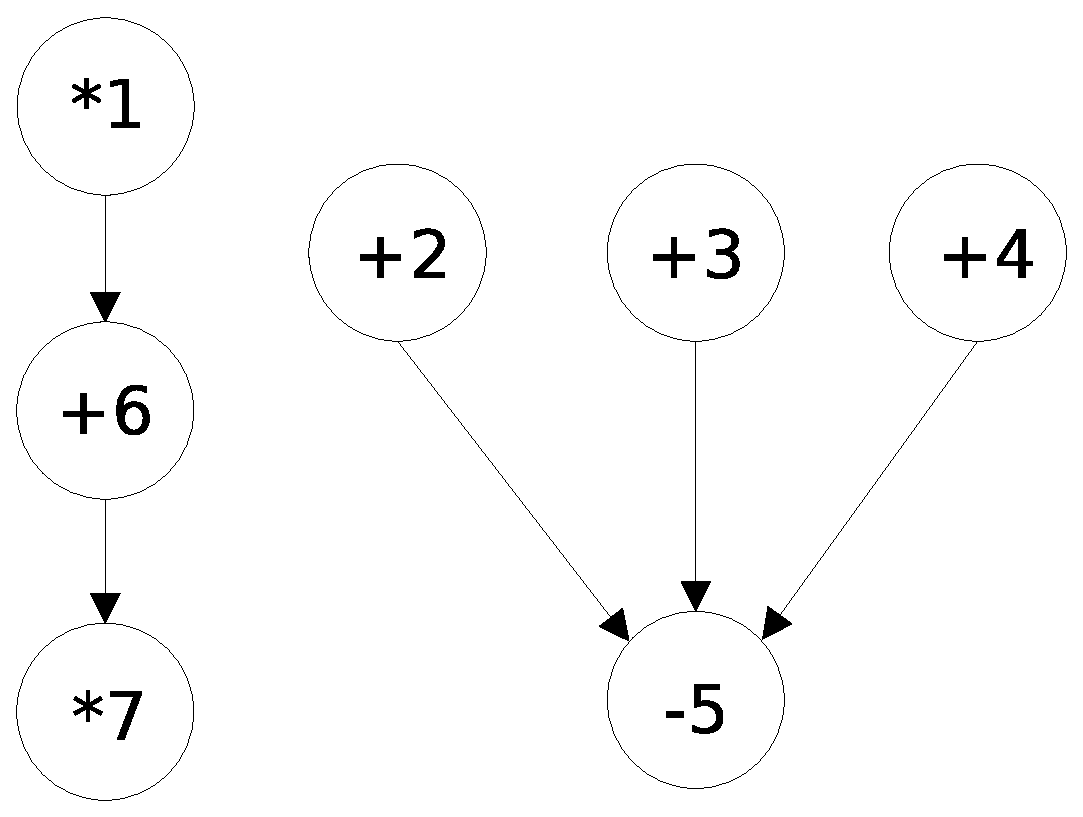
\includegraphics[scale = 0.22]{figures/Diagram1.eps}
}
}
}
\subfigure[Distribuzione di probabilit� e somma di probabilit�]{
\ifthenelse{\boolean{pdf}}
{
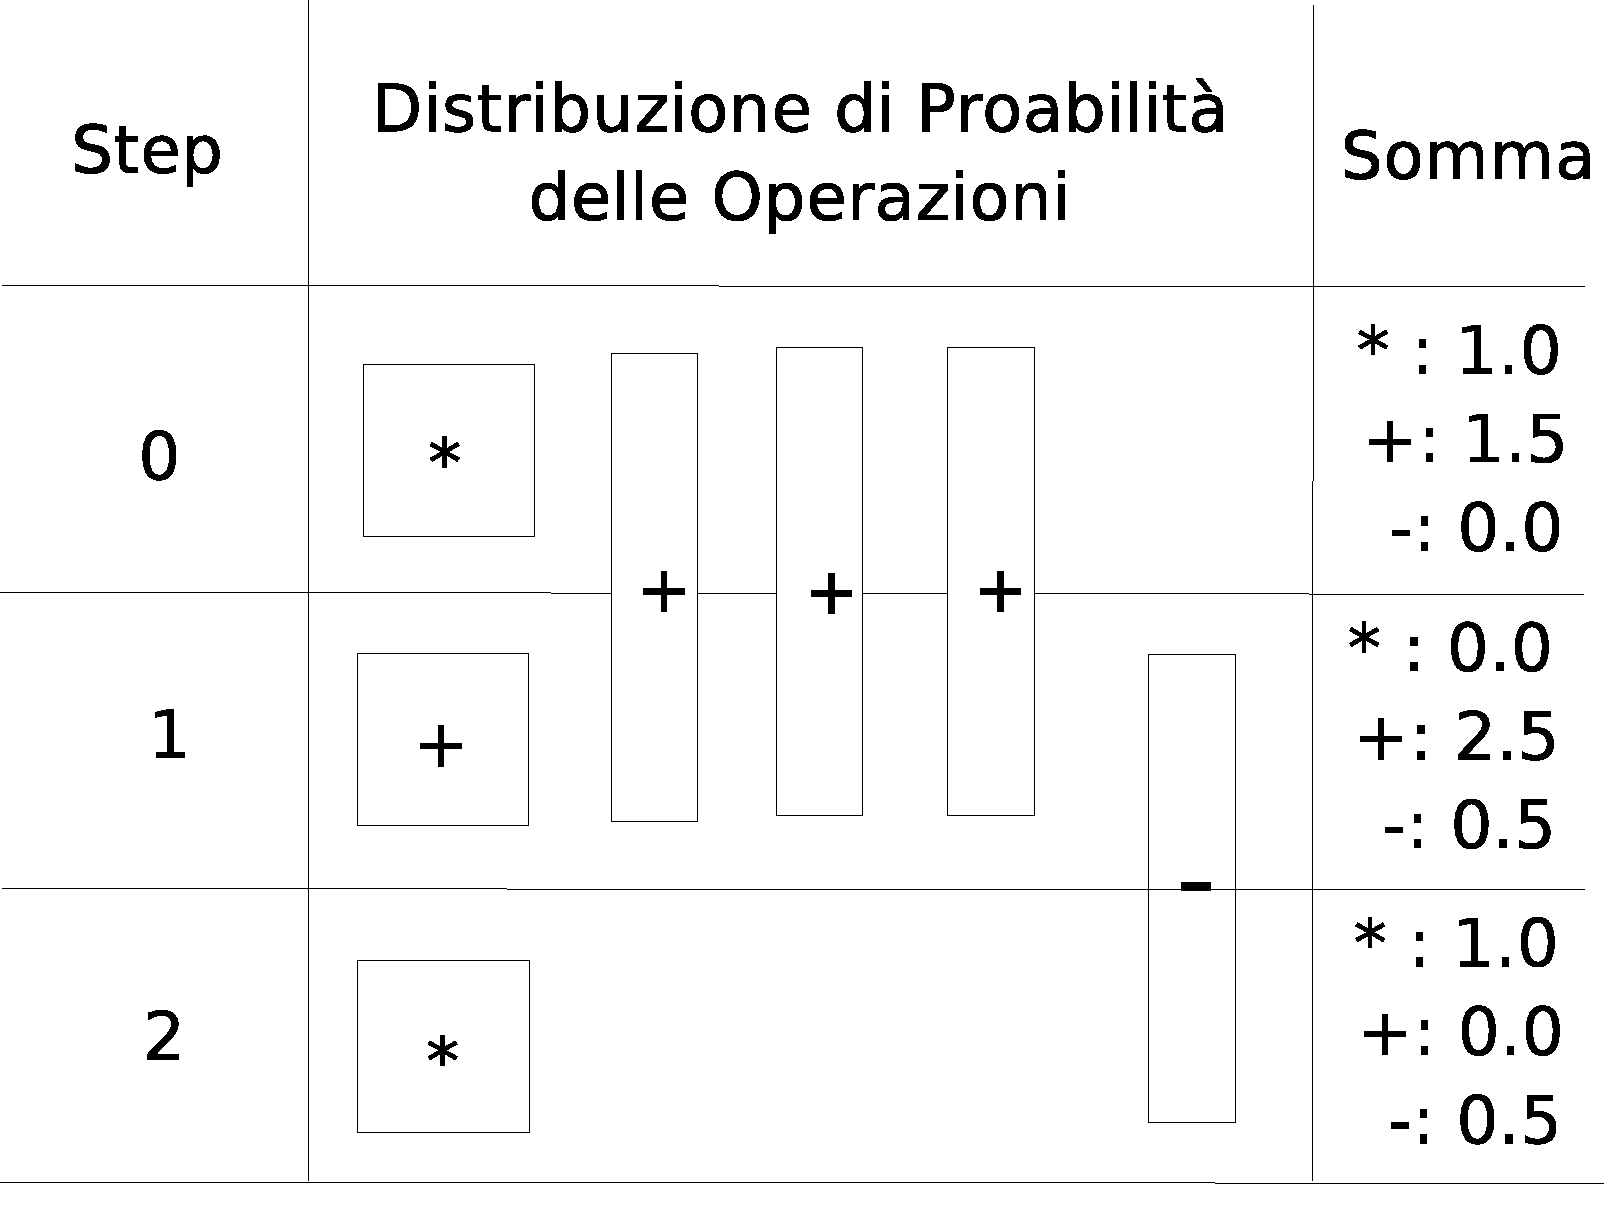
\includegraphics[scale = 0.2]{figures/Diagram2.pdf}
}{
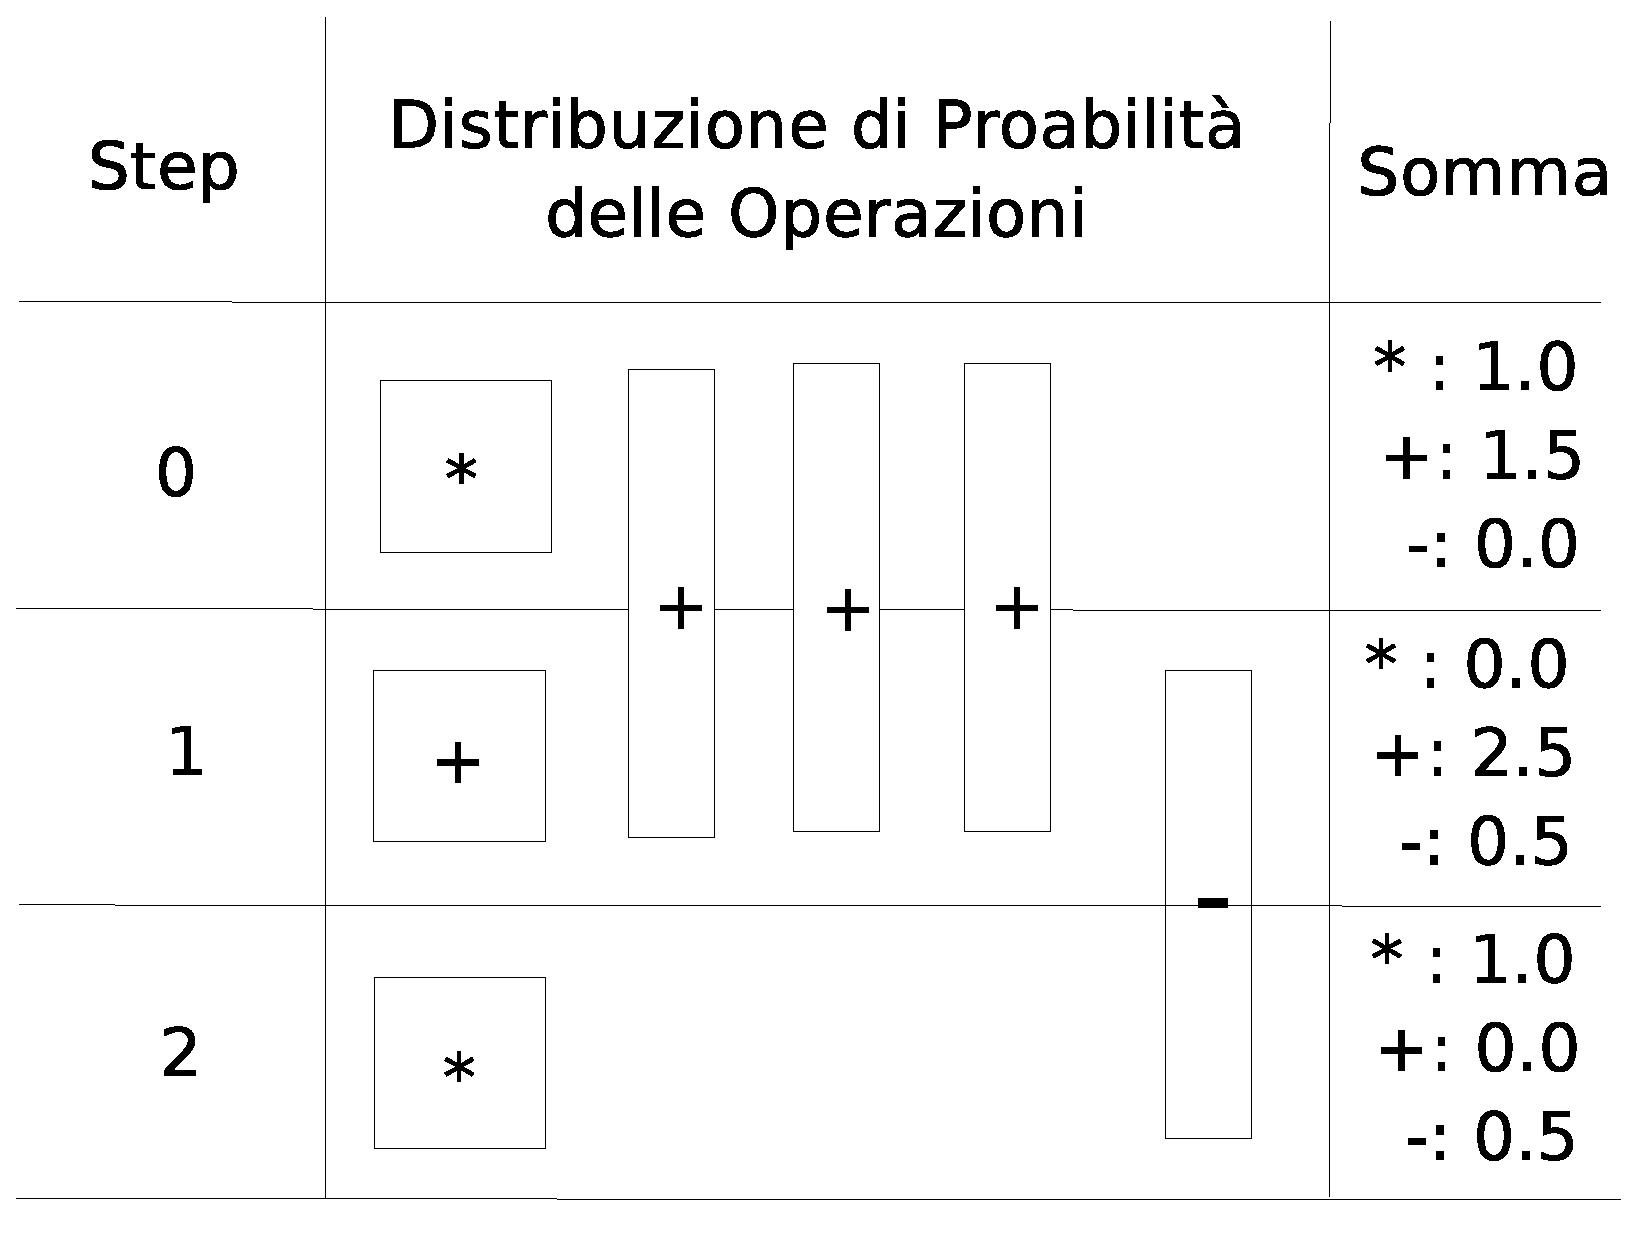
\includegraphics[scale = 0.2]{figures/Diagram2.eps}
}
}
\end{center}
\begin{center}
\subfigure[Tabella delle forze delle operazioni da schedulare \newline SF = self force \newline OF = predecessors' and successors' force \newline TF = total force]{
\label{f:ex:tab}
\begin{tabular}{|l|r||r|r|r|}
\hline 
Op & CS & SF & OF & TF \\
\hline
\hline
+2 & 0 & -0.50 & 0 & -0.50 \\
\hline
+2 & 1 & +0.50 & 0 & +0.50 \\
\hline
+3 & 0 & -0.50 & 0 & -0.50 \\
\hline
+3 & 1 & +0.50 & 0 & +0.50 \\
\hline
+4 & 0 & -0.50 & 0 & -0.50 \\
\hline
+4 & 1 & +0.50 & 0 & +0.50 \\
\hline
-5 & 1 & 0 & -1.50 & -1.50 \\
\hline
-5 & 2 & 0 & 0 & -0 \\
\hline
\end{tabular}
}
\end{center}
\begin{center}

\subfigure[Scheduling calcolato dall'Algoritmo Force Directed]{
\label{f:ex:fd}
\fbox{
\ifthenelse{\boolean{pdf}}
{
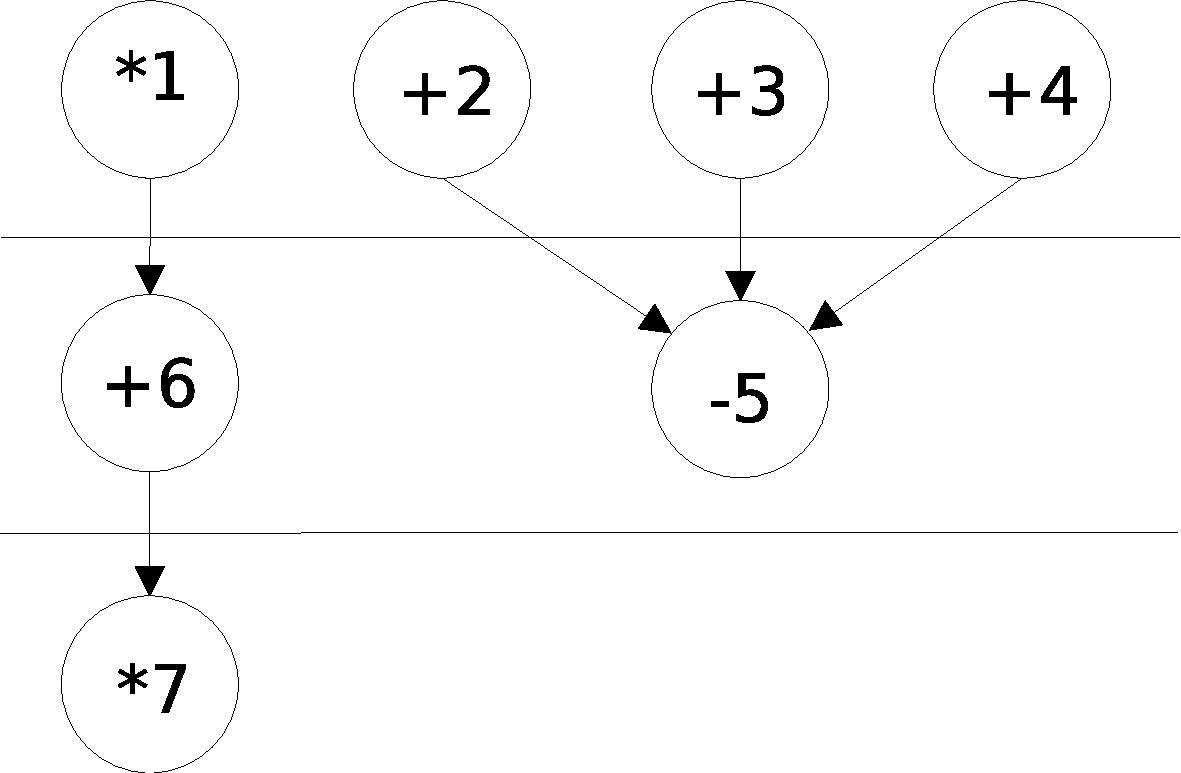
\includegraphics[scale = 0.2]{figures/Diagram3.pdf}
}{
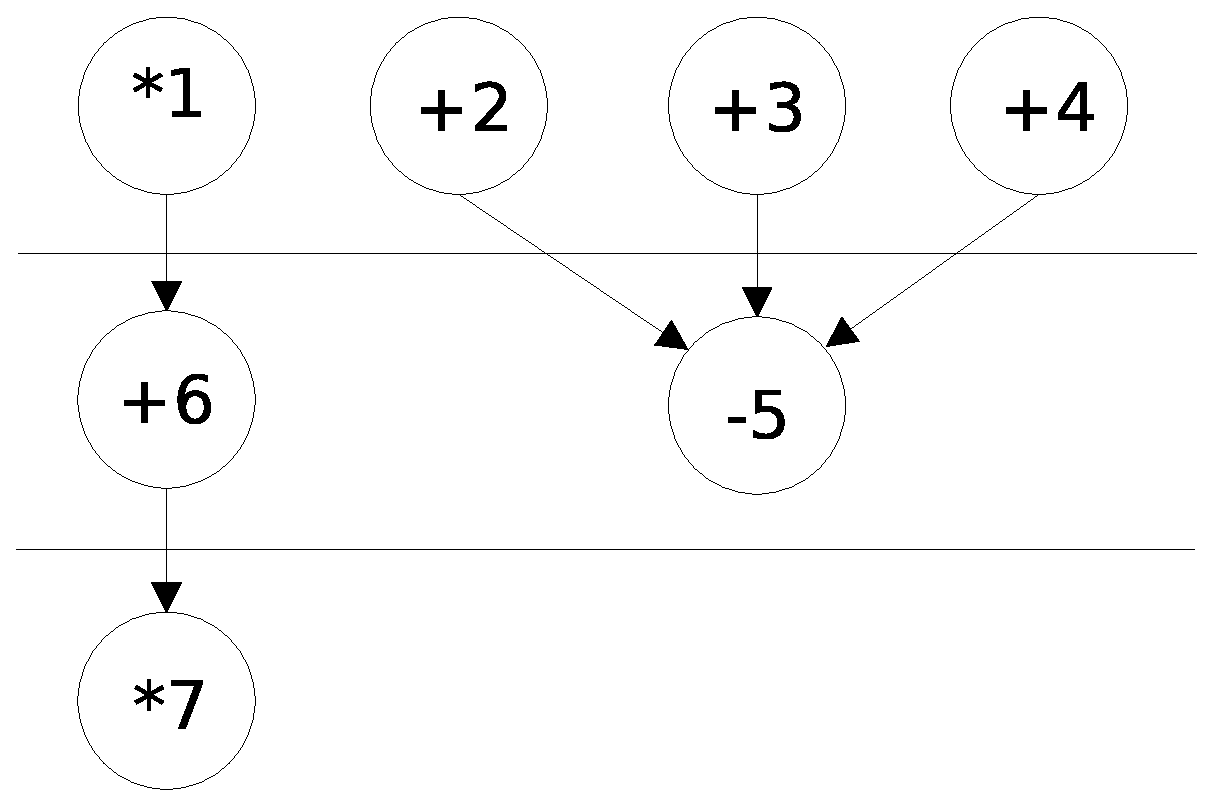
\includegraphics[scale = 0.2]{figures/Diagram3.eps}
}
}
}
\subfigure[Scheduling con risorse minime]{
\label{f:ex:hand}
\fbox{
\ifthenelse{\boolean{pdf}}
{
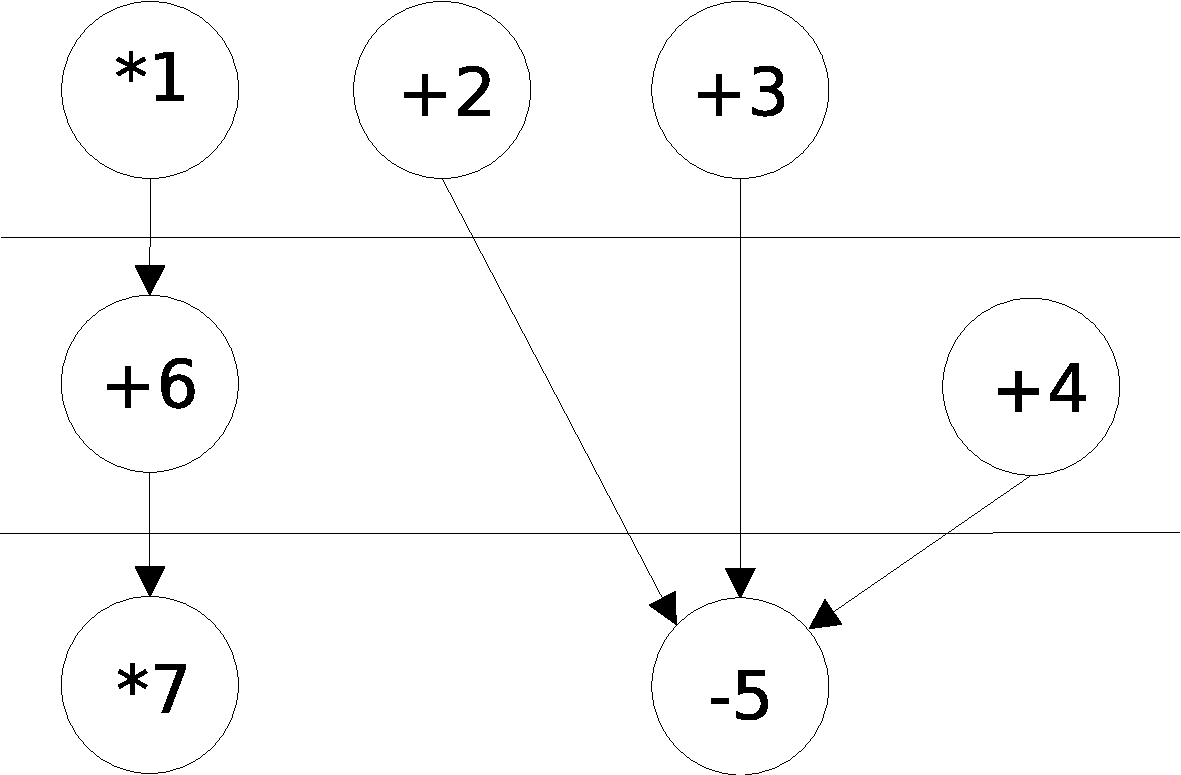
\includegraphics[scale = 0.2]{figures/Diagram4.pdf}
}{
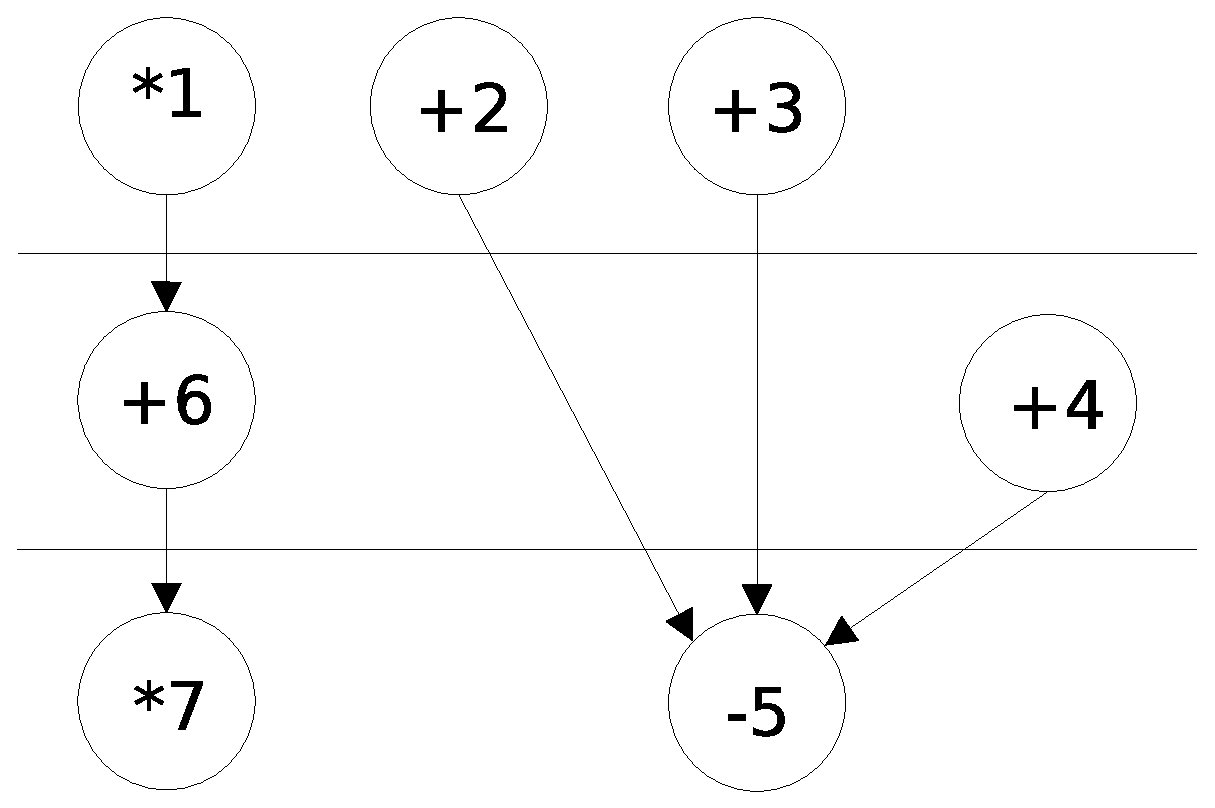
\includegraphics[scale = 0.2]{figures/Diagram4.eps}
}
}
}
\end{center}
\hcaption{Esempio delle limitazioni insite nel calcolo delle \emph{successors' and predecessors' forces}}

\label{f:ex}
\end{figure}


\subsection{Corpo dell'algoritmo}
\label{c:ori:core:body}
Dopo aver mostrato le singole fasi dell'algoritmo, � ora possibile illustrarlo nella sua completezza. L'algoritmo � iterativo ed ad ogni iterazione un'operazione viene assegnata ad un passo di controllo. Il numero massimo di iterazioni quindi � pari al numero di operazioni, ma pu� essere minore perch� � possibile assegnare in qualsiasi momento un'operazione che abbia mobilit� unitaria.

I passi da compiere ad ogni iterazione sono:
\begin{enumerate}
\item calcolare la finestra temporale delle operazioni tramite l'utilizzo di ASAP e ALAP e derivare da questa la loro mobilit� e quindi le distribuzioni di probabilit�;
\item aggiornare le somme di probabilit�;
\item calcolare le \emph{self-forces} per ogni assegnamento <operazione-passo di controllo> possibile;
\item aggiungere alle \emph{self-forces} le forze di predecessori e successori;
\item scegliere la coppia <operazione-passo di controllo> avente forza minore: aggiungere l'assegnamento allo scheduling.
\end{enumerate}


\subsection{Considerazioni sulla complessit�}
\label{c:ori:core:compl}
Viene ora analizzata la complessit� dell'algoritmo, considerando il caso pessimo, ricalcando quanto riportato in \cite{fd1} con alcune considerazioni ulteriori; con \emph{n} � indicato il numero di operazioni del problema, con \emph{c} il numero di passi di controllo previsto:
\begin{enumerate}
\item ad ogni iterazione dell'algoritmo almeno un'operazione viene schedulata (tipicamente pi� di una, ma si sta considerando il caso peggiore); il numero massimo di iterazioni dell'algoritmo � quindi pari ad \emph{n};
\item ad ogni iterazione vengono calcolate le forze di massimo \emph{n} operazioni;
\item per ognuna delle operazioni si devono calcolare \emph{h} forze dove \emph{h} � la mobilit� delle operazioni; nel caso peggiore la mobilit� corrisponde al numero totale di passi di controllo quindi \emph{h} = \emph{c};
\item Per calcolare una forza � necessario calcolare le forze relative a tutti i predecessori e successori che nel caso peggiore sono pari a \emph{n-1}; una considerazione non presente nell'analisi formulata da Paulin e Knight: per calcolare la forza relativa ad un predecessore o un successore si devono sommare i contribuiti relativi a ciascuno dei passi di controllo in cui l'operazione � schedulabile; quindi ricalcando le considerazione fatte nel passo precedente la complessit� va aumentata di un ulteriore fattore pari a \emph{c}.
\end{enumerate}

Da queste considerazioni si ricava che la complessit� dell'algoritmo � pari a $O(c^2 n^3)$. Tuttavia in questi calcoli non � stata considerata la possibilit� dell'esistenza di costrutti condizionali. In questo caso come illustrato in \ref{c:ori:core:prob} � necessario calcolare le somme di probabilit� considerando le reciproche mutue esclusioni. Questi calcoli devono essere ripetuti ad ogni iterazione per ogni passo di controllo. Affinch� il tempo per individuare il valore di queste somme sia trascurabile al fine di calcolare la complessit� dell'algoritmo � necessario che tali calcoli abbiano complessit� inferiore a $O(c n^2)$, tuttavia ne in \cite{fd1} ne in \cite{fd2} � riportato un metodo rapido con cui effettuarli. Un metodo verr� illustrato in \ref{c:impl:force:prob} avente complessit� pari a $O(b^4)$ ove \emph{b} � il numero di blocchi basici del problema.

Esistono delle semplificazioni all'algoritmo che comportano una riduzione della complessit�:
\begin{itemize}
\item limitare la mobilit� delle istruzioni ad un valore prefissato, ad esempio a 10 passi di controllo; la finestra temporale sar� centrata sul centro della finestra originaria; il tempo necessario ad effettuare la riduzione, che deve essere effettuata ad ogni iterazione, � $O(c n)$ quindi trascurabile rispetto alla complessit� del corpo dell'iterazione; nella complessit� propria dell'intero algoritmo quindi si pu� sostituire al termine \emph{c} il termine \emph{H} pari alla costante scelta come valore prefissato; la complessit� si riduce quindi a $O(H^2 n^3)$ ove H � fissato e minore di \emph{c};

\item utilizzare un modo diverso per valutare le \emph{predecessors' and successors' forces}; in particolare i tre tipi di forze sono calcolate in tre fasi successive; nella prima fase vengono calcolate e memorizzate tutte le \emph{self-forces}; nella seconda fase il SDG � attraversato dall'inizio alla fine e per ciascuna operazione la forza memorizzata � posta uguale alla propria \emph{self-force} sommata a quella dei predecessori; infine con una terza passata, questa volta dal basso verso l'alto, vengono sommate anche le forze dei successori; la complessit� complessiva scenderebbe secondo quanto riportato in \cite{fd1} a $O(c n^2)$, se si trascura la somma delle forze di predecessori e successori; infatti non trascurando questo aspetto, la complessit� si pu� calcolare come: \emph{n} iterazioni per \emph{n} operazioni per \emph{c} passi di controllo per \emph{$\log{cn}$} somme di forze di predecessori e successori per un totale di $O(c n^2 \log{cn})$ ; applicando la semplificazione del punto precedente si ottiene $O(H n^2 \log{Hn})$ con \emph{H} costante.
\end{itemize}


\section{Estensioni all'algoritmo proposte da Paulin e Knight}
\label{c:ori:longcore}
Sin dalla presentazione dell'algoritmo, Paulin e Knight illustrarono una serie di estensioni dell'algoritmo (oltre a quelle presentate in \ref{c:ori:core:compl} per ridurre la complessit�) per introdurre costrutti ciclici, per estendere le finalit� dell'algoritmo, per eliminare alcune delle limitazioni della versione base e per tentare di incorporare tecniche di \emph{look-ahead}.

\subsection{Scheduling con cicli}
\label{c:ori:longcore:cycle}
L'algoritmo descritto fino a questo momento � in grado di gestire tra i costrutti di controllo solo quelli di tipo condizionale. L'estensione che comprende la gestione dei costrutti iterativi (gestione dei cicli) parte dall'assunzione che nella descrizione comportamentale del sistema ad ogni ciclo venga assegnato un vincolo relativo alla durata temporale di una sua iterazione o al numero di unit� funzionali allocabili per la sua esecuzione. Nel primo caso il corpo del ciclo verr� schedulato separatamente utilizzando la versione base dell'algoritmo, nel secondo verr� invece utilizzato il \emph{force-directed list scheduling} (\ref{c:ori:longcore:vincoli}).

Nel caso di pi� cicli annidati, le operazioni relative a quello pi� interno verranno schedulate per prime, quindi il ciclo stesso ed in particolare una sua iterazione verr� considerata come un'unica operazione avente tempo di esecuzione pari alla durata di un'iterazione. Le operazioni esterne al ciclo non potranno essere schedulate contemporaneamente all'operazione rappresentante il ciclo intero. Questo processo � ripetuto per tutti i cicli finch� viene schedulato quello pi� esterno.

Per cercare di forzare il pipelining fra le diverse iterazioni del ciclo ed estrarre quindi un maggior parallelismo � possibile invece di schedulare le operazioni della singola iterazione, replicare tali operazioni un numero di volte pari al numero di iterazioni che si vuole vengano eseguite parallelamente. Una volta fatto ci� � sufficiente applicare l'algoritmo classico del Force Directed scheduling sulle operazioni originali e su quelle ottenute tramite la replicazione considerando oltre alle dipendenze originarie quelle presenti fra le operazioni appartenenti a iterazioni diverse.

\subsection{Estensioni allo scopo dell'algoritmo}
Lo scopo primario dell'algoritmo � quello di minimizzare l'utilizzo delle unit� funzionali utilizzate; tuttavia � facilmente utilizzabile per minimizzare altri tipi di risorse oltre alle unit� funzionali.

\subsubsection{Minimizzazione dei costi relativi ai bus}
Uno degli elementi che � possibile minimizzare utilizzando questo algoritmo sono i costi relativi ai bus all'interno dell'architettura sintetizzata. Schedulare un'operazione in un passo di controllo implica anche assegnare per quel passo di controllo un trasferimento di dati fra l'unit� funzionale e un registro (memorizzazione del risultato dell'operazione) e almeno un trasferimento da registro ad unit� funzionale (caricamento dei dati dell'operazione). Il numero minimo di interconnessioni necessario per sintetizzare uno scheduling sar� pari al massimo numero di trasferimenti presenti in un passo di controllo. Si pu� modellizzare l'utilizzo di un'interconnessione come l'utilizzo di un nuovo tipo di unit� funzionale. Per calcolare la probabilit� di questo tipo di "operazioni" in un passo di controllo � sufficiente considerare la probabilit� di ciascuna operazione di qualsiasi tipo in quel passo di controllo moltiplicata per il numero di interconnessioni distinte per quel tipo di operazione. Quindi per ottenere le somme di probabilit� per le interconnessioni � sufficiente applicare la formula:
\begin{equation}
Com\_DG(i) = \sum_{TypeOp} (DG(i,TypeOp) \cdot NofCon(TypeOp))
\end{equation}
ove
\begin{description}
\item[TypeOp] � il tipo di operazione;
\item[DG(i, TypeOp)] � la somma di probabilit� dell'i-esimo passo di controllo dell'operazione di tipo \emph{TypeOp};
\item[NofCon(TypeOp)] � il numero di connessioni dell'unit� funzionale che esegue le operazioni di tipo \emph{TypeOp}.
\end{description}

Nel calcolo delle \emph{self-forces} e delle \emph{predecessors' and successors' forces} bisogner� quindi aggiungere anche le forze relative alle connessioni calcolate allo stesso modo di quelle delle altre operazioni. In questo modo l'algoritmo tender� a minimizzare sia l'utilizzo di unit� funzionali, sia l'utilizzo delle connessioni. Se si vuole minimizzare solo il costo delle connessioni sar� sufficiente considerare solo le forze relative alle interconnessioni e trascurare le altre.

\subsubsection{Minimizzazione dei costi relativi ai registri}
Un secondo parametro che l'algoritmo pu� minimizzare all'interno dell'architettura � il costo totale dei registri che � pari al loro numero, il quale a sua volta corrisponde al numero massimo di archi di dipendenza dato che attraversano quella linea immaginaria che separa due diversi control step nel SDG schedulato. L'algoritmo applicato a questo problema non solo cerca di minimizzare l'utilizzo dei registri, ma fornisce anche ad ogni iterazione una stima del limite inferiore del numero di registri che sono necessari.

Anche in questa versione dell'algoritmo viene creato un nuovo tipo di operazioni che verr� chiamato \emph{operazione di memorizzazione}: ad ogni operazione che produce un risultato utilizzato da altre operazioni si associa una nuova operazione di tipo memorizzazione indipendentemente dal numero di operazioni che utilizzeranno tale risultato. Tale operazione rappresenta l'esistenza di una variabile in quel determinato passo di controllo. Come costruire la distribuzione di probabilit� di questo tipo di operazioni fittizie � tuttavia pi� complesso di quelle reali o di quelle create nel caso precedente. Nel caso sia l'operazione a monte, sia tutte le operazioni a valle siano state schedulate la distribuzione di probabilit� (in questo caso � improprio parlare di distribuzione di probabilit� perch� la somma dei diversi valori pu� essere superiore a uno, ma per affinit� si continuer� a chiamarla con questo termine) avr� valore unitario nei passi di controllo compresi fra quello dell'operazione che produce il dato escluso a quello dell'ultima operazione che lo utilizza incluso (cio� si modellizza che i registri, che nella pratica vengono utilizzati nel passaggio fra due passi di controllo, vengano utilizzati nel secondo passo di controllo della coppia a cavallo del passaggio). Negli altri passi di controllo la distribuzione di probabilit� varr� 0. Se una o pi� delle operazioni che individuano il tempo di vita della variabile associata all'operazione di memorizzazione non � schedulata, la creazione della distribuzione di probabilit� risulta pi� complessa, perch� a priori non si conosce quale sar� l'ultima operazione ad utilizzare il dato. Si stima quindi la vita media del dato utilizzando questa formula:
\begin{equation}
Tempo di Vita Medio = \frac{Asap + Alap + max}{3}
\end{equation}
dove 
\begin{itemize}
\item \emph{ASAP} � il tempo di vita della variabile nello scheduling ASAP;
\item \emph{ALAP} � il tempo di vita della variabile nello scheduling ALAP;
\item \emph{max} � il tempo di vita massimo calcolabile combinando $ASAP_{begin}$(inizio del tempo di vita nell'ASAP) e $ALAP_{end}$(fine del tempo di vita nell'ALAP) come $max=ALAP_{end} - ASAP_{begin} + 1$.
\end{itemize}

A questo punto i dati raccolti possono aver portato a due diverse situazioni:
\begin{enumerate}
\item i tempi di vita forniti da ALAP e ASAP sono disgiunti cio� $ASAP_{end} < ALAP_{begin}$;
\item i tempi di vita forniti da ALAP e ASAP si sovrappongono almeno parzialmente.
\end{enumerate}

Nel primo caso la distribuzione di probabilit� dell'operazione di assegnamento varr� $\frac{Tempo di Vita Medio}{max}$ nei passi di controllo compresi fra $ASAP_{begin}$ e $ALAP_{end}$, estremi inclusi e 0 negli altri passi di controllo. Nel secondo caso il sovrapporsi di passi di controllo in cui sia per l'ASAP che per l'ALAP una certa variabile sar� viva � indice del fatto che sicuramente con qualsiasi scheduling in quel passo di controllo la variabile sar� viva e quindi in quel passo la distribuzione di probabilit� dovr� valere uno. Inoltre questi dati forniscono un'ulteriore informazione: per quel passo di controllo sicuramente quella variabile sar� viva, quindi sar� necessario un registro per memorizzarla ed in questo modo si � ottenuto un'informazione riguardo il numero minimo di registri necessari, anche se magari nessuna operazione � stata ancora schedulata. Negli altri passi di controllo compresi fra $ASAP_{begin}$ e $ALAP_{end}$ ma non facenti parte della sovrapposizione, la distribuzione di probabilit� varr� $\frac{Tempo di Vita Medio - lunghezza della sovrapposizione}{max - lunghezza della sovrapposizione}$. Dalle distribuzioni di probabilit� si ricavano poi le somme di distribuzioni di probabilit�; a questo punto nel calcolo delle singole forze oltre al contributo delle \emph{self-forces} e delle \emph{predecessors' and successors' forces} delle operazioni canoniche, bisogner� tenere in considerazioni il contributo delle \emph{predecessors' and successors' forces} relative alle operazioni fittizie di memorizzazione utilizzando la formula canonica.

\subsection{Integrazione di informazioni relative all'architettura}
\label{c:ori:longcore:arch}
E' possibile sfruttare alcune informazioni relative all'architettura target per indirizzare l'algoritmo di scheduling. Il Force Directed � un algoritmo il cui scopo � minimizzare il numero di risorse utilizzate. In generale l'algoritmo non discrimina un tipo di unit� funzionale rispetto ad un altro, ma tende a minimizzare in maniera uniforme il numero di operazioni dei diversi tipi. Tuttavia il costo di allocazione delle unit� funzionali pu� variare sensibilmente a seconda delle funzionalit� implementate. Quindi pu� essere opportuno cercare di favorire la minimizzazione delle risorse pi� costose a scapito di quelle economiche. Un modo semplice ed efficace per indirizzare l'algoritmo di scheduling in questa direzione rendendo pi� critiche le operazioni pi� costose � moltiplicare le somme di probabilit� per un fattore indice del costo del particolare tipo di unit�. In questo modo l'algoritmo sar� portato a cercare di schedulare prima le operazioni relative a unit� funzionali con costo maggiore e quindi minimizzare con maggiore efficacia l'occupazione delle risorse pi� costose.

Una seconda informazione che � non solo possibile ma fortemente consigliato utilizzare all'interno del Force Directed per ottenere risultati migliori � quella relativa alla presenza di unit� funzionali che possono compiere diversi tipi di operazione come ad esempio le ALU. Per inserire questa informazione all'interno dei dati dell'algoritmo � sufficiente utilizzare in ogni passo di controllo al posto di una somma di probabilit� per ciascun tipo di operazione eseguibile dall'unit� multifunzionale un'unica somma che tenga conto delle probabilit� di tutte le operazioni assegnate a quel tipo di risorsa. Per ottenere questo valore non � sufficiente sommare le somme di probabilit� relative ai singoli tipi di operazione assegnati a quell'unit� funzionale: in questo modo infatti non si terrebbe conto della possibilit� che esistano mutue esclusioni fra le operazioni appartenenti alle diverse somme che portano ad un calcolo differente della somma di probabilit� come illustrato in \ref{c:ori:core:prob}; il metodo corretto per calcolare la somma di probabilit� relativa a unit� multifunzonali � invece sostituire tutte le operazioni assegnate a quel tipo di risorsa con un unico nuovo tipo fittizio, che per esempio potrebbe essere chiamato con il nome stesso del tipo di unit�, e proseguire nell'applicazione dell'algoritmo con i soliti passi. Questa semplificazione si pu� attuare per� a condizione che:
\begin{itemize}
\item nel caso si stia minimizzando il costo dei bus, le operazioni afferenti alla stesso tipo di unit� funzionale abbiano un numero uguale di ingressi;
\item le operazioni abbiano tempo di esecuzione e tempo di set-up relativo (confrontare quanto verr� esposto in \ref{c:ori:longcore:relax}) uguale tra loro.
\end{itemize}
In caso contrario non � possibile applicare la sostituzione e sar� necessario calcolare la somma di probabilit� dell'unit� funzionale multipla utilizzando le operazioni originarie e tenendone quindi in conto le caratteristiche.

\subsection{Rilassamento di alcune condizioni per l'applicazione dell'algoritmo}
\label{c:ori:longcore:relax}
Nella prima descrizione dell'algoritmo (\ref{c:ori:core}) si � posto come limitazione che tutte le operazioni venissero eseguite in un unico ed intero passo di controllo. Questa restrizione � tuttavia superabile ed in particolare l'algoritmo del Force Directed pu� considerare l'esistenza di operazioni concatenate (coppia o numero maggiore di operazioni eseguibili in sequenza all'interno del periodo di un passo di controllo e legate da dipendenze di dato), operazioni multiciclo (operazioni che necessitano di pi� passi di controllo per essere eseguite e che durante tutti i passi di controllo rendono indisponibile la risorsa) e operazioni eseguite da unit� funzionali pipeline.

\subsubsection{Scheduling con Chaining}
Per permettere scheduling con chaining verr� aumentata la mobilit� calcolata con ASAP e ALAP: l'ASAP verr� anticipato di uno o pi� passi di controllo se � possibile concatenare l'operazione in oggetto con una o pi� delle operazioni precedenti e simmetricamente l'ALAP verr� posticipato di uno o di pi� passi di controllo se � possibile concatenare l'operazione in oggetto con una o pi� successive. Per determinare se ci sono delle operazioni concatenabili si associa ad ogni operazione la sua latenza, quindi si esegue l'ASAP memorizzando per ogni operazione la somma delle latenze del percorso critico precedente quell'operazione (in pratica all'ASAP basato sui passi di controllo si affianca l'ASAP basato sui tempi di esecuzione). Confrontando l'ASAP di un'operazione basato sui tempi di esecuzione sommato al tempo di esecuzione proprio dell'operazione (per cos� dire l'ASAP del termine e non dell'inizio dell'operazione) con gli ASAP temporali dei predecessori, se la differenza di questi valore � inferiore alla durata del priodo di un passo di controllo allora questa coppia di operazioni, e quelle eventualmente comprese fra di esse nel SDG, possono essere concatenate cio� schedulate nello stesso passo di controllo.

\subsubsection{Scheduling di operazioni multiciclo}
Cos� come il Force Directed prevede la possibilit� del concatenamento delle operazioni, esso prevede anche la possibilit� di schedulare operazioni che richiedano pi� di un passo di controllo per essere eseguite (operazioni multiciclo). Le modifiche da applicare all'algoritmo sono:
\begin{itemize}
\item Calcolo della mobilit�

Le uniche differenze che si deve tenere in conto nel calcolo della mobilit� sono quelle previste negli algoritmi ASAP e ALAP considerando anche operazioni con latenza superiore al singolo passo di controllo; tuttavia � possibile combinare questa caratteristica con quella della concatenazione delle operazioni; le catene di operazioni concatenate in questo caso potranno occupare pi� di un passo di controllo, ma per semplificare le strutture di controllo e il calcolo dell'utilizzo delle unit� funzionali si considera solo il caso in cui per schedulare la catena di operazioni sia necessario un numero di passi di controllo comunque pari a quello necessario a schedulare l'operazione pi� lunga della catena; cio� data un'operazione con tempo di esecuzione superiore a quello del ciclo di controllo, ma che non � multiplo della durata del ciclo stesso, si cercher� di concatenare ad essa una o pi� operazioni per eventualmente sfruttare il tempo rimanente a disposizione nel primo o nell'ultimo o in entrambi i passi di controllo dello scheduling dell'operazione lunga; l'utilizzo della concatenazione deve comunque essere considerato come una possibilit� da valutare e non come un'imposizione in quanto scopo dell'algoritmo � la minimizzazione delle risorse e non del tempo totale di esecuzione e la concatenazione non necessariamente riduce il numero di risorse necessarie.

\item Calcolo delle distribuzioni di probabilit�

Cos� come nel caso dei registri, anche la distribuzione di probabilit� di operazioni multiciclo perde la propriet� matematica di avere somma unitaria. La somma delle distribuzioni di probabilit� di un'operazione multiciclo sar� infatti pari al numero stesso di cicli necessari per eseguire l'operazione. Un'operazione con mobilit� unitaria e tempo di esecuzione pari a n passi di controllo avr� distribuzione di probabilit� cos� impostata: 1 nell'unico passo di controllo in cui � assegnabile l'operazione, ma 1 anche negli n-1 passi successivi. Per operazioni aventi mobilit� non nulla il calcolo � pi� complesso: in pratica � come se le si scomponessero in un numero di frazioni pari al numero di passi di controllo necessari ad eseguirle e si creasse una distribuzione di probabilit� per un'operazione nella sua completezza non direttamente ma costruendo prima una distribuzione di probabilit� per ciascuna delle frazioni create. Una volta fatto ci� la distribuzione di probabilit� relativa all'operazione complessiva si ottiene sommando per ogni passo di controllo i contributi relativi alle singole frazioni dell'operazione. La distribuzione di probabilit� della prima frazione � quella che si avrebbe nel caso di un'operazione normale cio� un valore pari a $ \frac{1}{mobilita'}$ per ogni passo di controllo tra l'ASAP e l'ALAP della operazione estremi compresi. Le successive frazioni dell'operazione devono essere schedulate nei passi successivi consecutivi a quello della prima frazione, quindi le corrispondenti distribuzioni di probabilit� saranno uguali a quelli della prima frazione ma traslate opportunamente in avanti di un numero di passi di controllo pari all'indice della frazione meno uno.
\end{itemize}

Una volta applicate queste modifiche � possibile applicare normalmente l'algoritmo.

\subsubsection{Scheduling su unit� pipelined}
L'introduzione della possibilit� di utilizzare unit� funzionali dotate di pipeline � molto semplice. Si considera che le operazioni eseguite da esse occupino la risorsa e quindi vengano logicamente schedulate solo nel primo ciclo della loro esecuzione. Dal punto di vista dell'algoritmo quindi un'operazione di questo tipo verr� trattata esattamente come un'operazione che possa venir eseguita in un unico passo di controllo. Un'altra interpretazione possibile � quella di considerarla come un'operazione multiciclo ma porre uguale a zero la probabilit� che le frazioni successive alla prima vengano schedulate in qualsiasi passo di controllo. Chi dovr� fare distinzione di questo tipo di operazioni e tenere conto del ritardo fra il momento in cui un'operazione viene schedulata e il momento in cui si rende disponibile il suo risultato alle operazioni successive sono gli algoritmi ASAP e ALAP nel corso del calcolo delle finestre temporali e della mobilit�.

\subsection{Estensione con vincoli sulle risorse}
\label{c:ori:longcore:vincoli}
\subsubsection{Il \emph{force-directed list scheduling}}
Paulin e Knight hanno proposto un metodo per utilizzare il meccanismo del calcolo delle forze per realizzare uno scheduling con vincoli sulle risorse che punti a minimizzare i passi di controllo ovvero un algoritmo duale di quello fin qui illustrato. L'algoritmo illustrato prende il nome di \emph{Force-Directed List Scheduling} in quanto � una composizione dell'algoritmo Force-Directed e dell'algoritmo \emph{List-Based} (\ref{c:art:sch:time:lb}).

L'approccio del \emph{force-directed list scheduling} � simile a quello del \emph{list-based} tradizionale: la differenza sostanziale consiste nella funzione di priorit� utilizzata; nel caso in un passo di controllo il numero di operazioni di un certo tipo pronte e quindi schedulabili sia superiore al numero di risorse disponibili � necessario scegliere di quali operazioni posticipare lo scheduling; la funzione di priorit� utilizzata � la forza relativa al restringimento della finestra temporale dell'operazione da quella attuale ad una che escluda il passo di controllo corrente; le operazioni con forza minore sono quelle che se ritardate non aumenterebbero la congestione nell'utilizzo delle unit� funzionali nei passi successivi a quello corrente o lo farebbero in misura minore. Una volta calcolato quale operazione ha forza minore, essa viene posticipata; se vi fossero ancora troppe operazioni pronte ad essere schedulate non si sceglier� l'operazione con forza minore gi� calcolata fra quelle sopravvissute, ma sar� necessario prima di effettuare una nuova scelta ricalcolare le forze interessate e ripetere questo procedimento finch� abbastanza operazioni siano state posticipate. Il ricalcolo � reso non superfluo dal fatto che modificando la mobilit� di un'operazione vengono modificate anche le mobilit� dei suoi successori, cosa che pu� modificare il valore delle forze delle operazioni pronte. Il posticipare le operazioni non implica automaticamente che esse assumano priorit� maggiore rispetto a quelle passibili di scheduling a partire dal passo di controllo successivo e che esse vengano quindi schedulate nel passo di controllo successivo. Nel caso infatti nel passo successivo non vi fossero nuovamente abbastanza unit� funzionali disponibili per soddisfare tutte le operazioni pronte si dovr� ricorrere nuovamente al calcolo delle forze per le operazioni in conflitto. Rimane da illustrare come calcolare le forze. Infatti a differenza dell'algoritmo presentato in \ref{c:ori:core} (l'algoritmo nella sua versione base) non si hanno informazioni riguardo alla mobilit� delle operazioni, ne riguardo al numero totale di passi di controllo necessari. Paulin e Knight hanno deciso di utilizzare per questo valore la lunghezza in passi di controllo del percorso critico corrente (esso pu� infatti aumentare se una delle operazioni critiche � stata posticipata). Stabilito questo valore si applicano gli algoritmi ASAP e ALAP (utilizzando sempre come numero di passi di controllo quello relativo al percorso critico) e quindi si ricavano finestre temporali e mobilit�. Evidenziate queste particolarit� si pu� riassumere i passi principali dell'algoritmo:
\begin{enumerate}
\item porre il numero di passi controllo pari alla lunghezza del percorso critico misurato in numeri di cicli di controllo;
\item per ogni passo di controllo:
\begin{enumerate}
\item calcolare con ASAP e ALAP le finestre di tempo delle operazioni;
\item determinare le operazioni che sono pronte nel passo di controllo corrente (operazioni i cui predecessori sono gi� state schedulati nei passi di controllo precedenti);
\item finch� il numero di operazioni pronte di un certo tipo supera il numero di unit� funzionali che possono eseguire quel particolare tipo di operazione;
\begin{enumerate}
\item se tutte le operazioni appartengono al percorso critico il numero totale di passi di controllo deve essere incrementato di un'unit� e quindi tutte le finestre temporali dovranno essere ricalcolate;
\item calcolare le forze dovute al posporre le operazioni del tipo in oggetto;
\item posticipare lo scheduling dell'operazione con minor forza;
\item rimuovere l'operazione dalla lista di quelle pronte;
\end{enumerate}
\item schedulare nel passo di controllo corrente tutte le operazioni pronte.
\end{enumerate}
\end{enumerate}

Questo approccio combina l'alto utilizzo delle unit� funzionali, la bassa complessit� computazionale ($O(n^2)$ nel caso pessimo, $O(n)$ mediamente) e la valutazione globale di tutti gli effetti collaterali di assegnare un'operazione ad un passo di controllo.

Un modo per sfruttare appieno questa versione dell'algoritmo � quella di utilizzarlo in combinazione con la formulazione originale: in una prima fase si fissa una stima del numero di passi di controllo necessari allo scheduling se esso non � gi� stato fissato come requisito dell'implementazione che si vuole ottenere; utilizzando questo dato si applica l'algoritmo Force Directed, in particolare integrandovi informazioni relative all'architettura come mostrato in \ref{c:ori:longcore:arch}, per ottenere una stima del numero minimo di unit� funzionali necessarie per schedulare tutte le operazioni. A questo punto si applica il force-directed list scheduling utilizzando come numero di risorse quello appena stimato per verificare se non fosse possibile ottenere uno scheduling in un numero di passi di controllo inferiore. Questa combinazione dei due algoritmi permette quindi di esplorare lo spazio di progetto, seppure in due passate, cercando di minimizzare due metriche diverse, tempo e area, che sono solitamente in contrapposizione.

\subsubsection{Calcolo del Numero di Passi di Controllo per Tentativi}
Esiste un'altra proposta di Paulin e Knight per utilizzare il Force Directed scheduling con vincoli sulle risorse per minimizzare il numero di passi di controllo. La struttura di questa versione dell'algoritmo � la seguente: si individua con ASAP e ALAP il numero minimo di passi di controllo necessario allo scheduling e si applica l'algoritmo classico su questi dati. Se durante la sua esecuzione si verifica che la stima (non il valore relativo alle operazioni gi� schedulate) di utilizzo di un tipo di unit� funzionale superasse il numero di unit� effettivamente disponibili, si incrementa di un'unit� il numero di passi di controllo totale e conseguentemente si incrementa di uno anche la mobilit� di tutte le operazioni estendendone la finestra temporale. Ci� viene applicato non solo alle operazioni ancora da schedulare, ma anche a quelle gi� schedulate i cui assegnamenti vengono cos� eliminati. Le finestre temporali risultano comunque pi� piccole di quelle che si otterrebbero applicando inizialmente ASAP e ALAP con numero di passi di controllo pari a quello attuale. In questo modo si ha un aumento del tempo di esecuzione dell'algoritmo, ma tendenzialmente  non significativo perch� la sua complessit� rimane inalterata in quanto le finestre temporali non vengono ricalcolate, ma semplicemente estese.

\subsection{Introduzione di vincoli temporali locali}
In alcune classi di applicazioni esistono dei vincoli temporali fra coppie di operazioni cio� vincoli sul tempo minimo e massimo che debba intercorrere fra le due computazioni. Questa richiesta � modellizzabile all'interno del Force Directed inserendo delle finte operazioni temporizzanti nel SDG fra le due operazioni incriminate ed associando a queste operazioni fittizie un intervallo di tempo. Esse in un certo senso servono solo come prememoria: non verranno mai schedulate, ma verranno tenute in considerazione per il calcolo delle finestre temporale delle operazioni che collegano, in modo tale che tali finestre rispettino i vincoli memorizzati nell'operazione temporizzante.

\subsection{Tecniche di look-ahead}
\label{c:ori:longcore:look}
Per le caratteristiche dell'algoritmo Force Directed, il costo in termini di complessit� temporale di utilizzare tecniche di look-ahead non � compensato dai minimi guadagni ottenibili con esse. Tuttavia gli autori stessi hanno proposto un'approssimazione di una tecnica di look-ahead (confrontare \ref{c:art:back:la}) che non comporta un aggravio della complessit� dell'algoritmo, ma che ne migliora, a dire degli autori, considerevolmente l'efficienza. L'idea in questo caso � di utilizzare all'interno della formula per il calcolo delle \emph{self-forces} non il valore attuale della somma di probabilit�, ma una media pesata fra quello attuale e quello che assumer� dopo l'assegnamento; nel dettaglio la formula utilizzata �: \[Force(i) = DG\_temp(i) \cdot x(i)\] dove 
\begin{description}
\item[Force(i)] � il contributo alla forza dello scheduling relativo all'i-esimo passo di controllo;
\item[DG\_temp(i)] � la somma di probabilit� del tipo di unit� funzionale che pu� eseguire l'operazione nell'i-esimo passo di controllo modificata per tenere in considerazione la situazione futura in questo modo: $DG\_temp(i)=DG(i)+x(i)/3$;
\item[x(i)] � la variazione della probabilit� dell'operazione nell'i-esimo passo di controllo a seguito dello scheduling.
\end{description}

Tuttavia svolgendo la formula si ottiene \[Force(i) = (DG(i) \cdot x(i)) + ((x(i))^2)/3\]
Il primo termine � presente gi� nella prima formulazione, quindi soffermandosi sul secondo si pu� notare che la differenza fra la forza calcolata nel modo tradizionale e quella calcolata con quest'ultimo metodo � pari a \begin{equation}
\vartriangle Self\-Force = \sum_i \frac{x^2(i)}{3}
\end{equation}

Analizzando questa formula � immediato constatare che essa non dipenda dalle somme di probabilit� ma solamente dalle variazioni nelle distribuzioni di probabilit� dell'operazione  nei vari passi. Queste variazioni non dipendono dagli specifici passi di controllo in cui � possibile schedulare l'operazione, ne dallo specifico passo in cui si sceglie di assegnare l'operazione o dal suo tipo ma unicamente dalla mobilit� posseduta da essa. La formula pu� essere quindi riscritta in questo modo, indicando con \emph{m} la mobilit� dell'operazione prima dello scheduling:
\begin{equation}
\vartriangle Self\-Force  = \frac{(\frac{m-1}{m})^2 - (m-1)(\frac{1}{m})^2}{3} = \frac{(m^2 - 3m + 2)}{3m^2}
\end{equation}

Quello che si � ottenuto � quindi una correzione delle \emph{self-force} che dipende unicamente dalla mobilit� dell'operazione in esame e che quindi non influenza direttamente la scelta del passo di controllo di una certa operazione, ma tuttalpi� l'ordine in cui viene scelta la prossima operazione da assegnare.
\chapter{Il Force Directed Scheduling proposto}
\label{c:my}
\thispagestyle{empty}

\vspace{0.5cm}

In questo capitolo verranno illustrate le modifiche apportate all'algoritmo originale del \emph{Force Directed scheduling}. Nella prima sezione verranno mostrate le variazioni applicate ai passi dell'algoritmo originario basate sulle osservazioni fatte nel capitolo precedente per ottenere migliori risultati in termini di numero di risorse allocate o di tempi di esecuzione minori. Nella seconda sezione verr� mostrata la versione proposta dell'algoritmo che consente di considerare contemporaneamente vincoli temporali e vincoli tecnologici a differenza delle estensioni proposte dagli autori che prevedevano la presenza di vincoli di un unico tipo.

\section{Proposte di modifiche all'algoritmo originale}
\label{c:my:var}
Le variazioni che verranno di seguito descritte sono state ipotizzate a seguito dell'analisi e delle critiche fatte alla versione originale dell'algoritmo di cui sono stati evidenziati (in particolare in \ref{c:ori:core:force}, \ref{c:ori:core:body} e \ref{c:ori:longcore:look})) i limiti insiti nel gestire particolari soluzioni.

\subsection{Priorit� delle operazioni}
\label{c:my:var:priority}
Il \emph{Force Directed scheduling} � un algoritmo che presenta una complessit� computazionale relativamente elevata rispetto ad algoritmi pi� semplici quali l'ASAP, l'ALAP o il List Based. Questa maggiore complessit� � da ascriversi principalmente alla visione pi� globale che questo algoritmo ha rispetto a quelli citati. Esso infatti per decidere un assegnamento deve tenere conto di tutti gli effetti secondari che tale assegnamento avrebbe nei diversi passi di controllo. Inoltre non segue un ordine prefissato nel scegliere quale operazione schedulare e quindi necessita che ad ogni iterazione le informazioni relative a tutte le operazioni vengano ricalcolate. E' evidente se si confronta questo sistema con quello per esempio del List Based in cui vengono considerate ad ogni passo di controllo solo le operazioni considerate pronte quanto questo comporti un dilatarsi dei tempi di calcolo.

Gli autori stessi dell'algoritmo (come mostrato in \ref{c:ori:core:compl} - considerazioni sulla complessit�) hanno cercato soluzioni che ne riducessero la complessit� limitando le finestre temporali delle operazioni. La soluzione qui presentata prevede invece una riduzione del numero di candidate ad essere schedulate in ogni iterazione, in modo tale che l'algoritmo dovendo scegliere solo da un sottoinsieme di operazioni, debba calcolare le forze solo relativamente a questo sottoinsieme. Terminato di assegnare le operazioni del sottogruppo prescelto si selezioner� un nuovo sottogruppo e cos� via sino ad esaurire tutte i sottogruppi e quindi tutte le operazioni. Questa limitazione applicata alla versione completa dell'algoritmo pu� essere anche combinata con quella proposta in \ref{c:ori:core:compl} per ottenere un'ulteriore riduzione della complessit� a spesa della bont� dei risultati. Il problema di ridurre il numero delle candidate raggruppandole in sottogruppi pu� essere modellizzato assegnando ad ogni operazione una priorit�: ad ogni iterazione verranno calcolate solo le forze delle operazioni con priorit� maggiore che saranno le possibili candidate ad un assegnamento. Rimane da determinare come scegliere le priorit� cio� quali operazioni raggruppare in modo tale che vengano schedulate in successione. Per far questo si pu� considerare che alla base del Force Directed scheduling c'� il calcolo degli effetti che ha un assegnamento di un'operazione su tutte le altre operazioni in tutti i passi di controllo.

Tuttavia ci si pu� chiedere se effettivamente un assegnamento abbia un'influenza significativa cos� estesa. Nella realt� si pu� facilmente evincere che se due operazioni sono molto distanti nel SDG l'assegnamento di una non influenzer� i possibili assegnamenti dell'altra o lo far� in misura minore. Una prima indicazione su come raggruppare l'operazioni � quindi quella data dalla loro vicinanza all'interno del SDG: operazioni vicine avranno finestre temporali sovrapposte e quindi concorreranno per l'utilizzo delle unit� funzionali negli stessi passi di controllo. Questo purch� le operazioni non siano in mutua esclusione reciproca, cio� non appartengano per esempio al ramo then e al ramo else di un costrutto condizionale. Infatti nel caso le operazioni siano in mutua esclusione, esse non saranno in concorrenza per l'assegnamento di unit� funzionali quindi si pu� pensare di schedularle in momenti diversi e perci� assegnarli a gruppi diversi.

Infine � possibile fare una considerazione sulle operazioni di salto condizionale: esse costituiscono per cos� dire dei paletti che fissano lo scheduling di tutte le altre operazioni, sia perch� tipicamente hanno bassa mobilit� facendo parte dei percorsi critici o dei rami ad essi pi� vicini, sia perch� molte operazioni hanno una dipendenza di controllo da esse.

Sulla base di questa serie di considerazioni si � scelto di utilizzare come suddivisione delle operazioni quella fornita dai blocchi basici che ovviamente rispetta sia il fatto di raggruppare operazioni vicine nei SDG, sia il fatto di raggruppare operazioni non in mutua esclusione reciproca. Questa suddivisione ha tuttavia la limitazione di essere di fatto nulla nel caso di assenza di costrutti condizionali. In questo caso l'algoritmo non si discosta dalla versione originale. In \ref{c:my:vincoli:priority} (priorit� delle operazioni in presenza di vincoli) verr� mostrato un possibile ordinamento parziale dei blocchi basici e quindi dei sottogruppi, ma tale ordinamento ha il solo scopo di diminuire i tempi di esecuzione in presenza di vincoli tecnologici: allo stato attuale non si ha indicazione se tale ordinamento offra risultati migliori, peggiori o complessivamente non confrontabili di un ordinamento completamente casuale. Individuare il migliore ordinamento dei blocchi basici � infatti a tutt'oggi ancora un problema insoluto. In mancanza di certezze viene ora utilizzato l'ordinamento parziale mostrato in \ref{c:my:vincoli:priority} in quanto � plausibile ritenere che questo ordinamento provocando un minore numero di violazioni di vincoli in quel caso per le ragioni ivi riportate, produca nel caso privo di vincoli risultati tendenzialmente migliori; come verr� illustrato l'ordinamento � parziale. Per renderlo totale si utilizzer� come seconda chiave della funzione di ordinamento (la prima � appunto la posizione nell'ordinamento parziale) una funzione che ordini in modo fissato ma casuale i blocchi basici.

\subsection{Interpretazione sulla formula della forza}
\begin{figure}
\begin{center}

\subfigure[SFG di esempio]{
\label{f:ex2:a}
\fbox{
\ifthenelse{\boolean{pdf}}
{
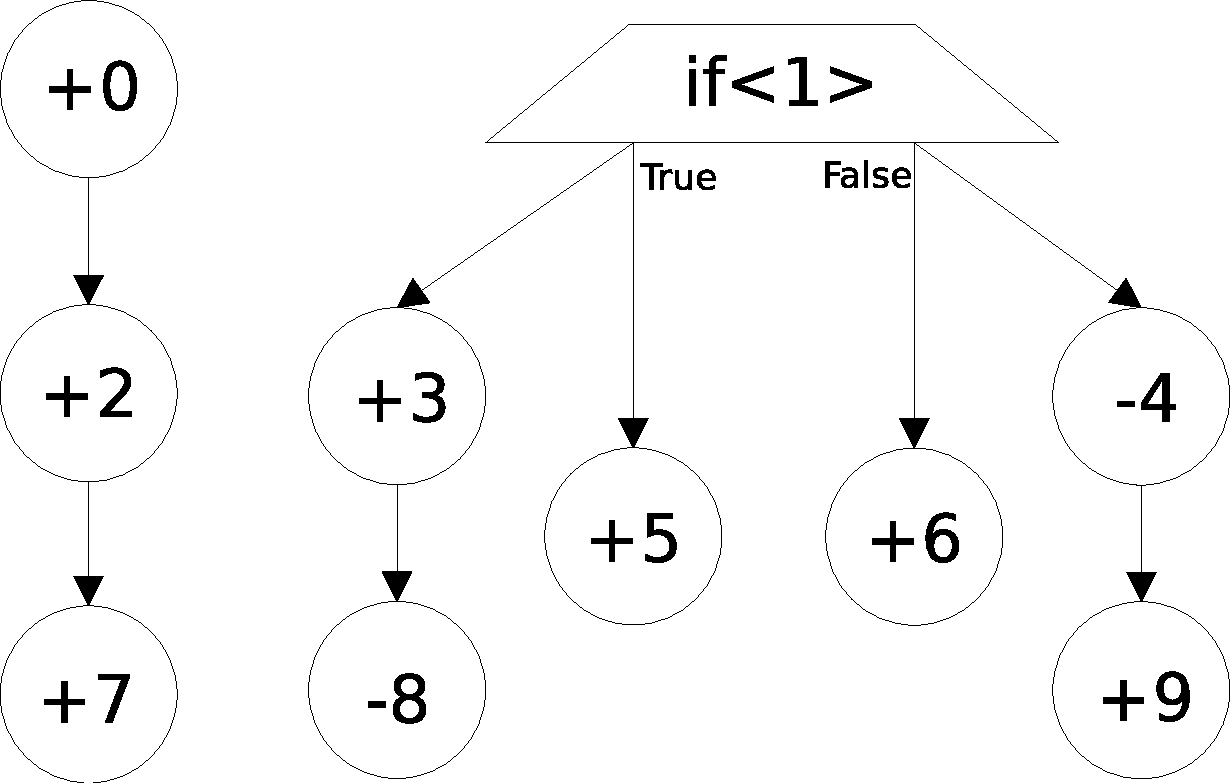
\includegraphics[scale = 0.22]{figures/Diagram5.pdf}
}{
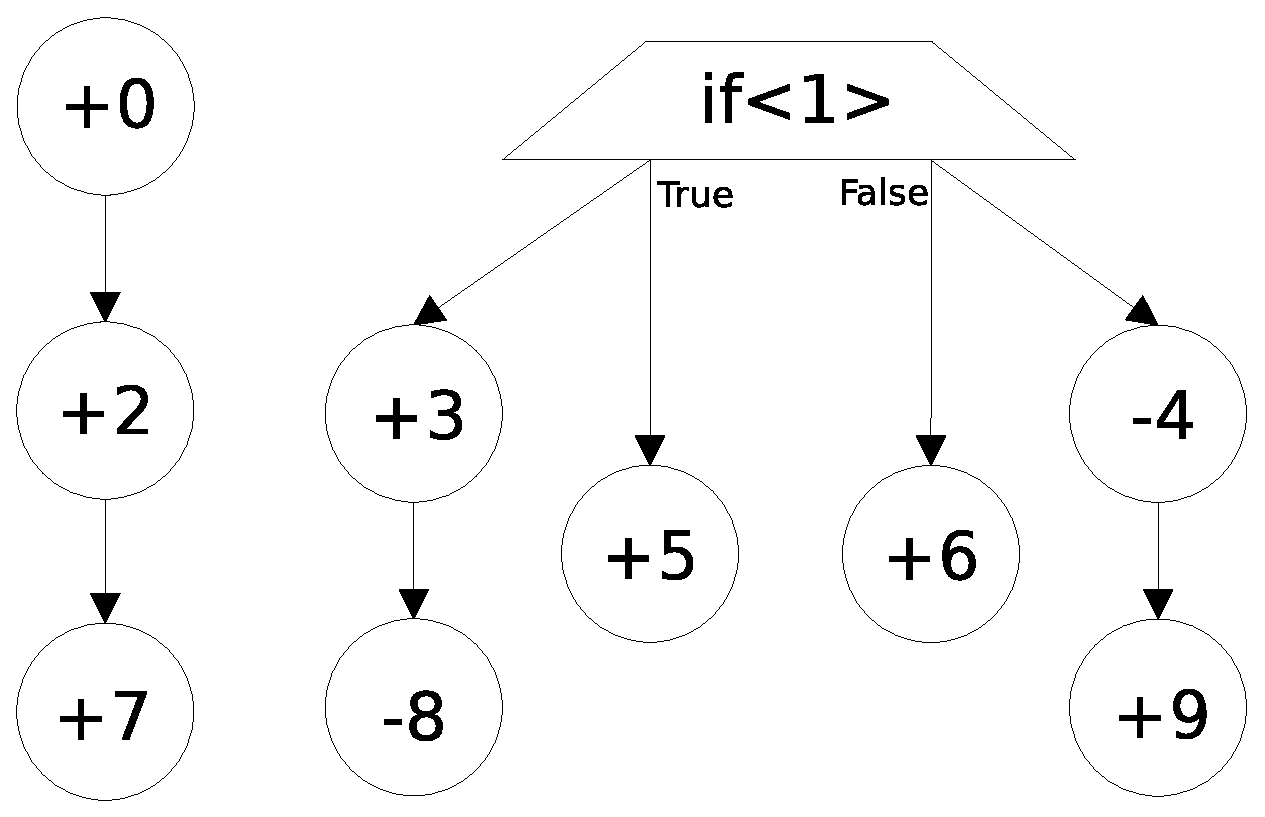
\includegraphics[scale = 0.22]{figures/Diagram5.eps}
}
}
}
\subfigure[Distribuzione di probabilit� e somma di probabilit�]{
\label{f:ex2:b}
\ifthenelse{\boolean{pdf}}
{
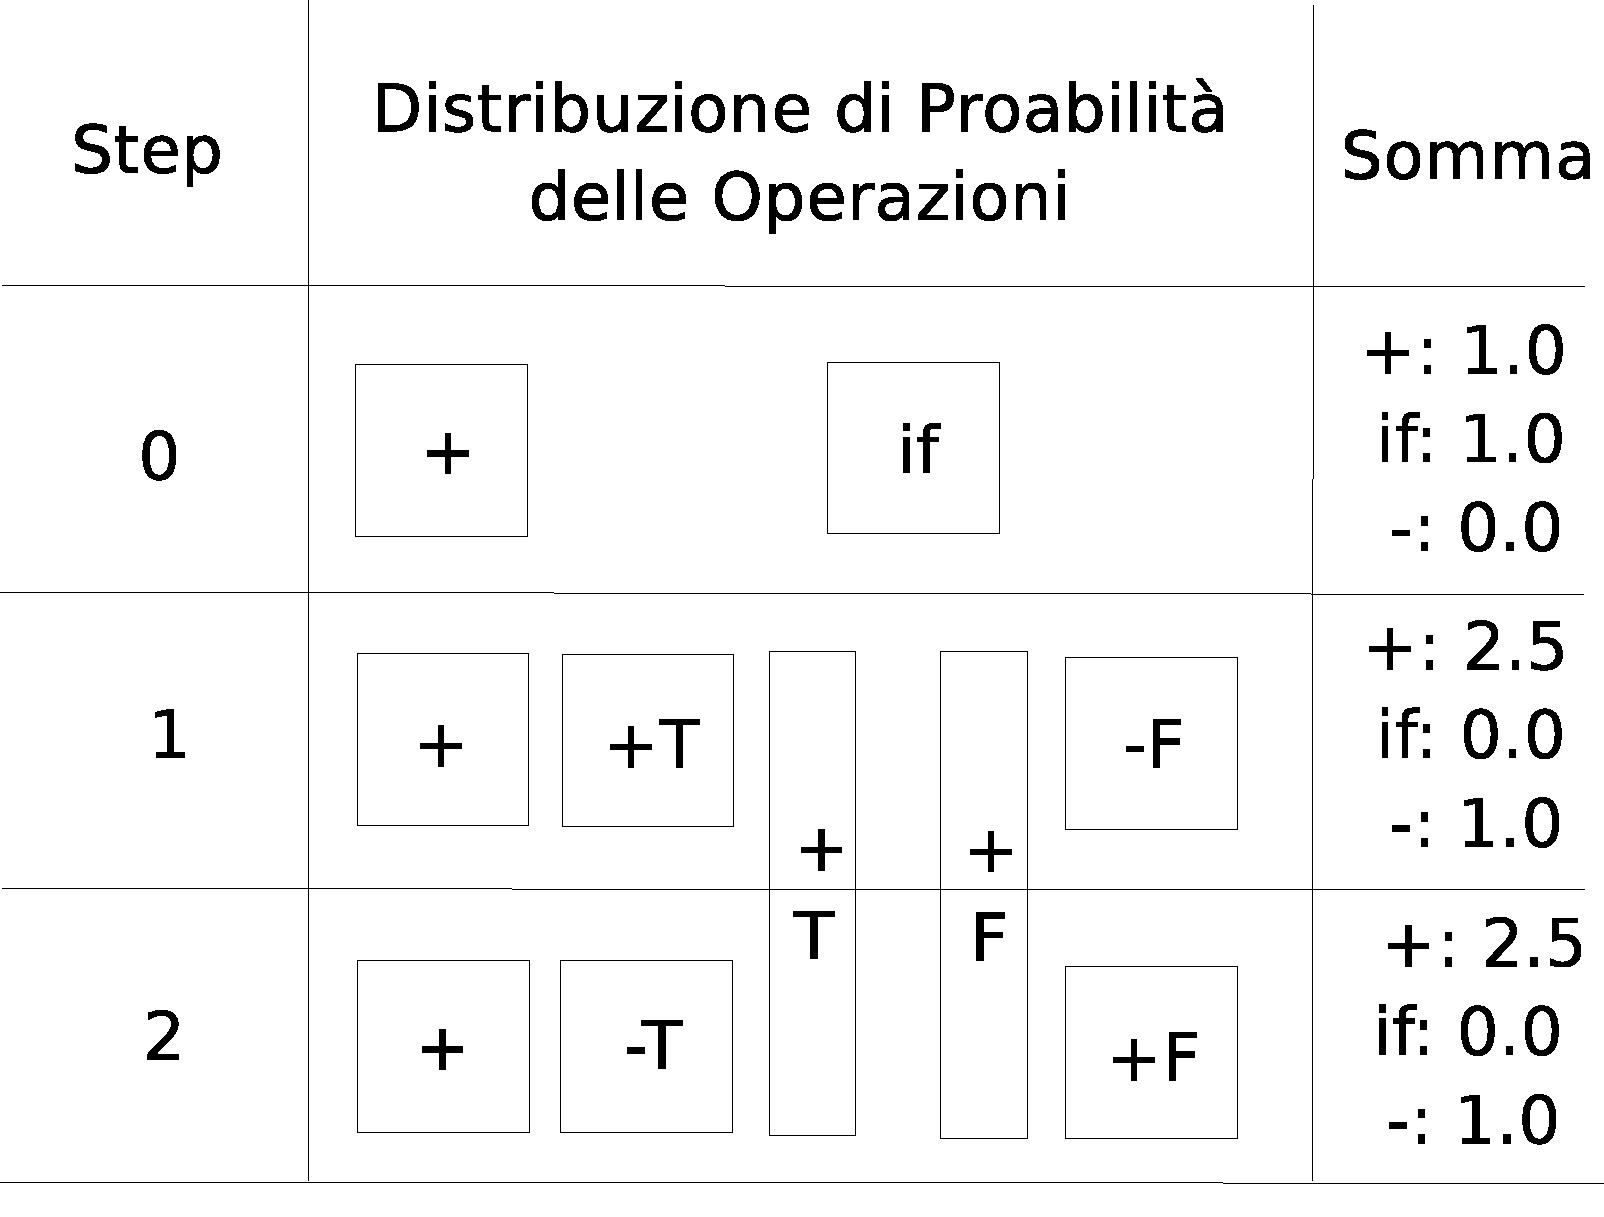
\includegraphics[scale = 0.22]{figures/Diagram6.pdf}
}{
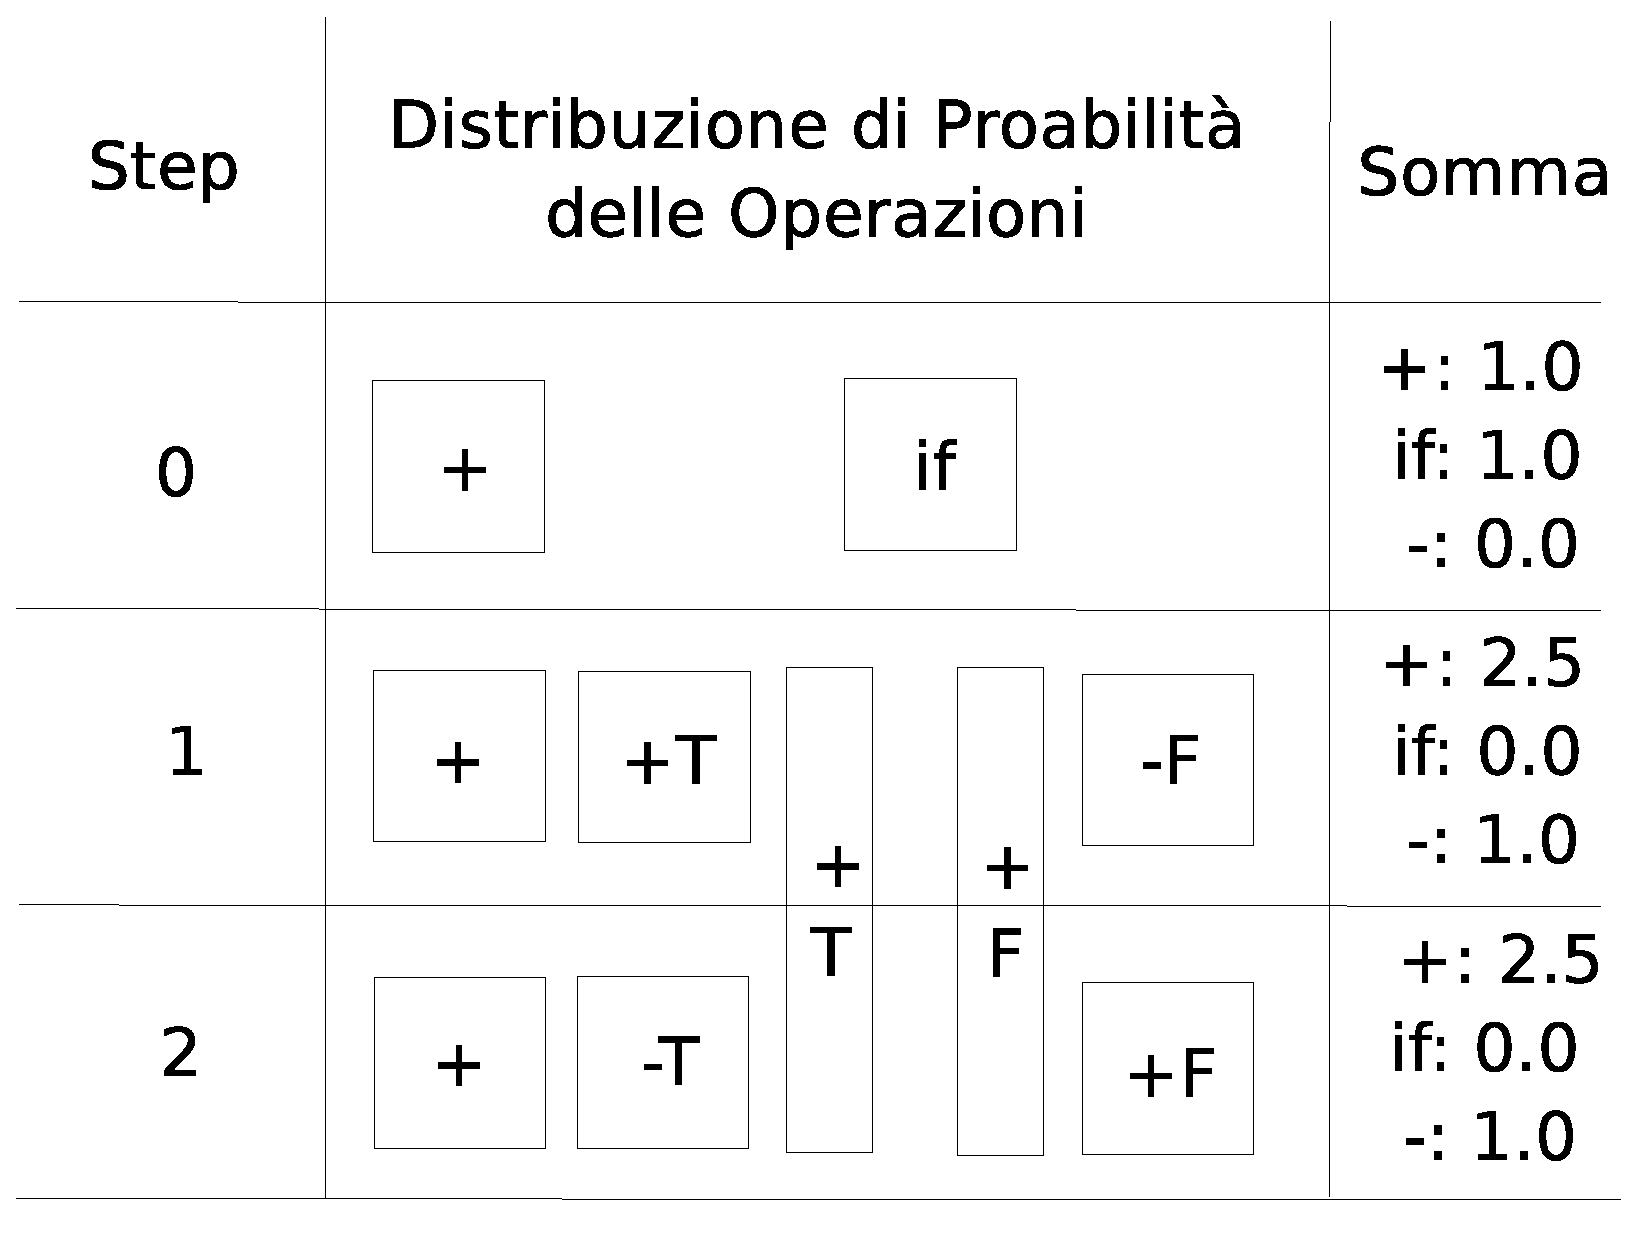
\includegraphics[scale = 0.22]{figures/Diagram6.eps}
}
}
\end{center}
\begin{center}
\subfigure[Tabella delle forze delle operazioni da schedulare \newline SF = self forces \newline OF = predecessors' and successors' forces \newline TF = total forces ]{
\label{f:ex2:tab}
\begin{tabular}{|l|r||r|r|r|}
\hline 
Op & CS & SF & OF & TF \\
\hline
\hline
+5 & 1 & 0.0 & 0.0 & 0.0 \\
\hline
+5 & 2 & 0.0 & 0.0 & 0.0 \\
\hline
+6 & 1 & 0.0 & 0.0 & 0.0 \\
\hline
+6 & 2 & 0.0 & 0.0 & 0.0 \\
\hline	
\end{tabular}
}
\end{center}
\begin{center}
\subfigure[Esempio di possibile scheduling prodotto dal Force Directed - caso pessimo]{
\label{f:ex2:ca}
\fbox{
\ifthenelse{\boolean{pdf}}
{
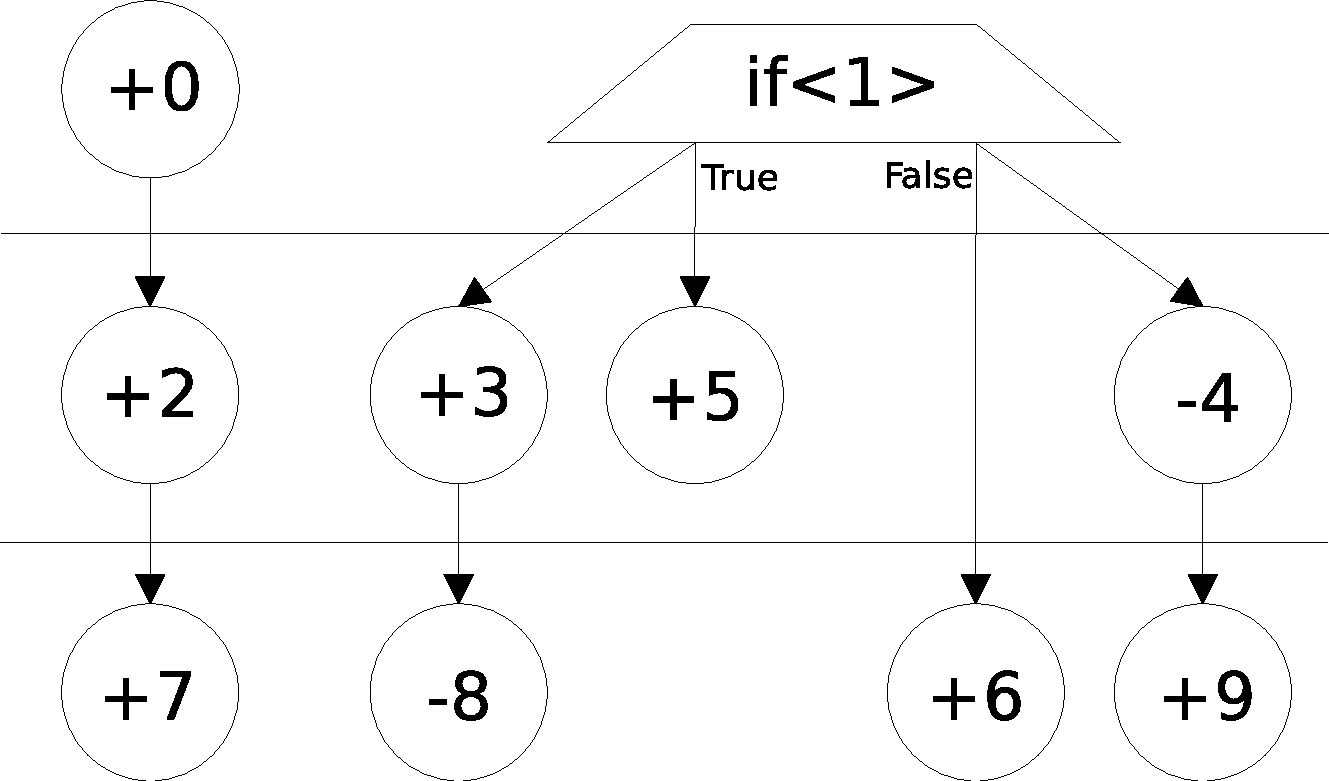
\includegraphics[scale = 0.22]{figures/Diagram7.pdf}
}{
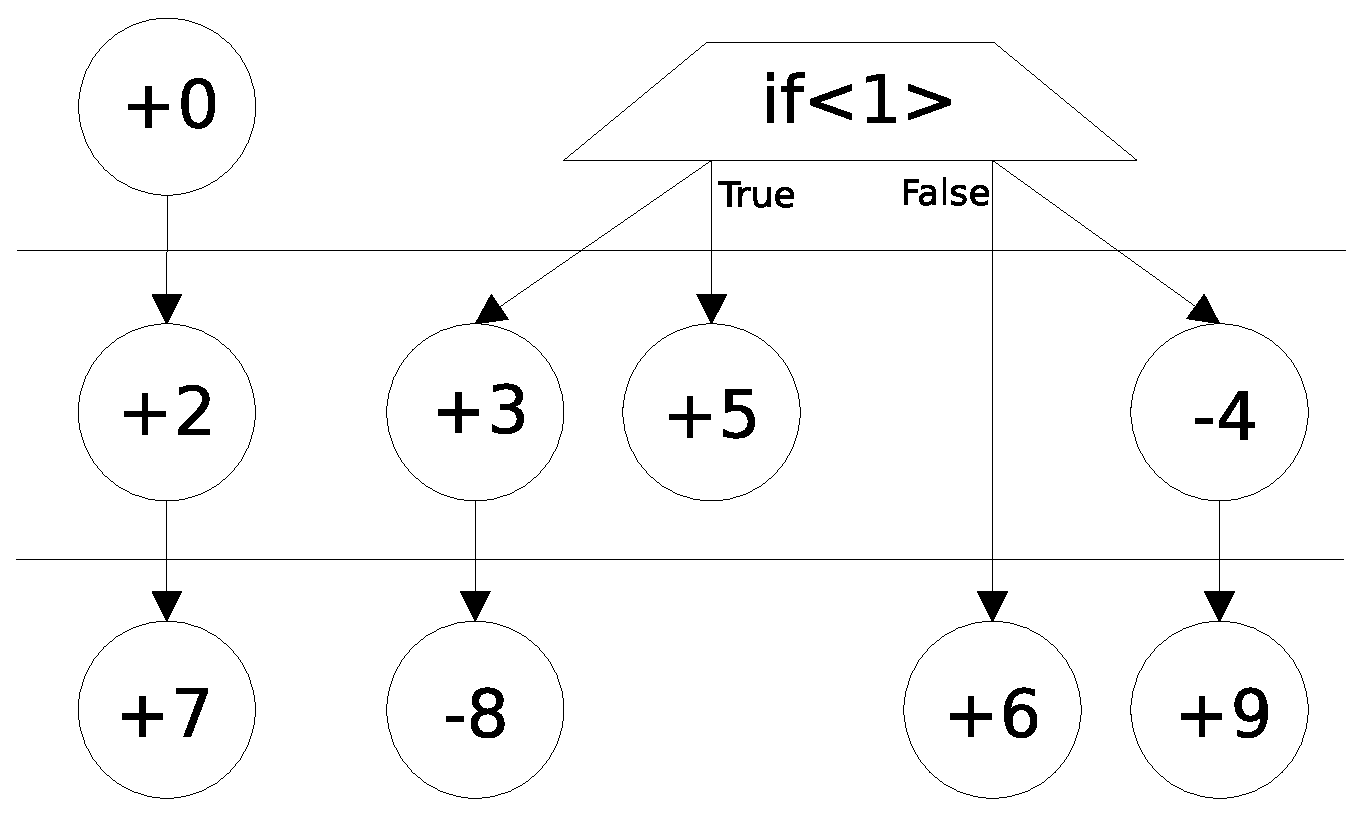
\includegraphics[scale = 0.22]{figures/Diagram7.eps}
}
}
}
\subfigure[Esempio di possibile scheduling prodotto dal Force Directed - caso ottimo]{
\label{f:ex2:cb}
\fbox{
\ifthenelse{\boolean{pdf}}
{
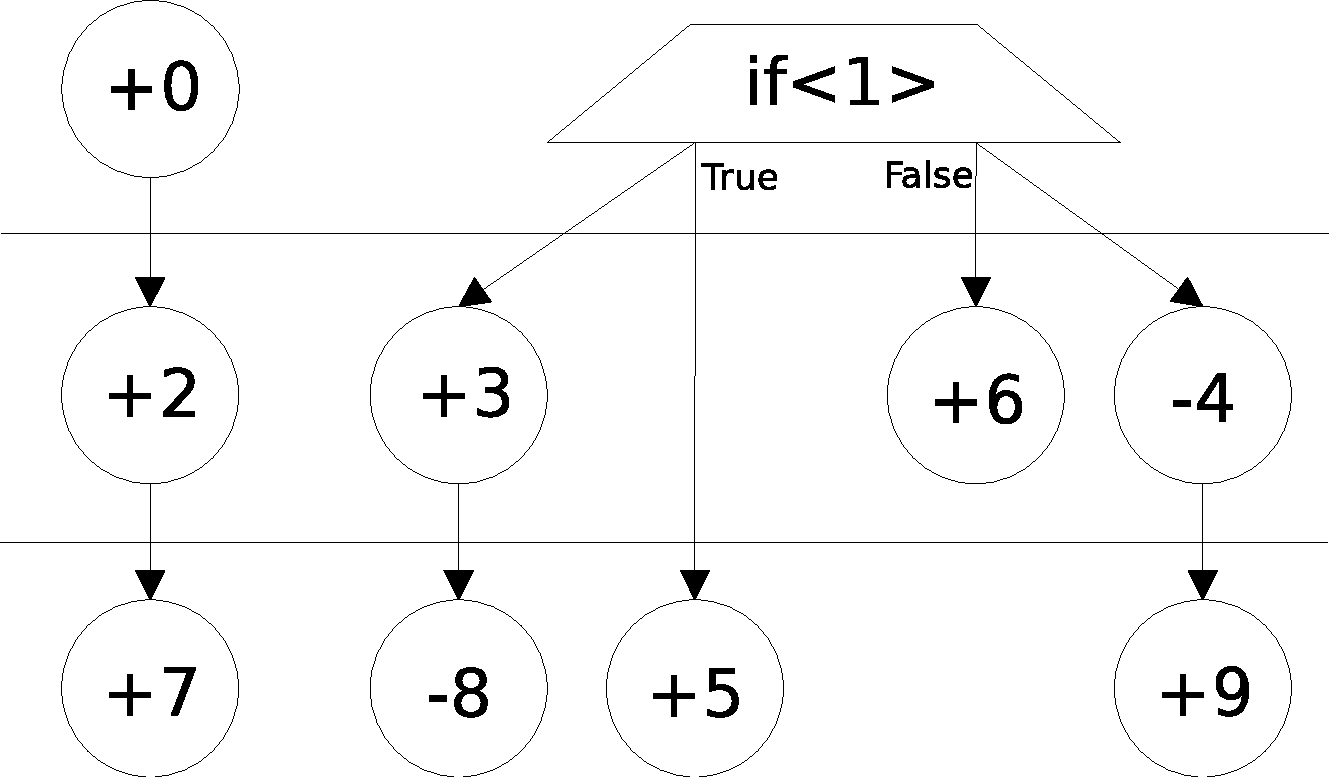
\includegraphics[scale = 0.22]{figures/Diagram8.pdf}
}{
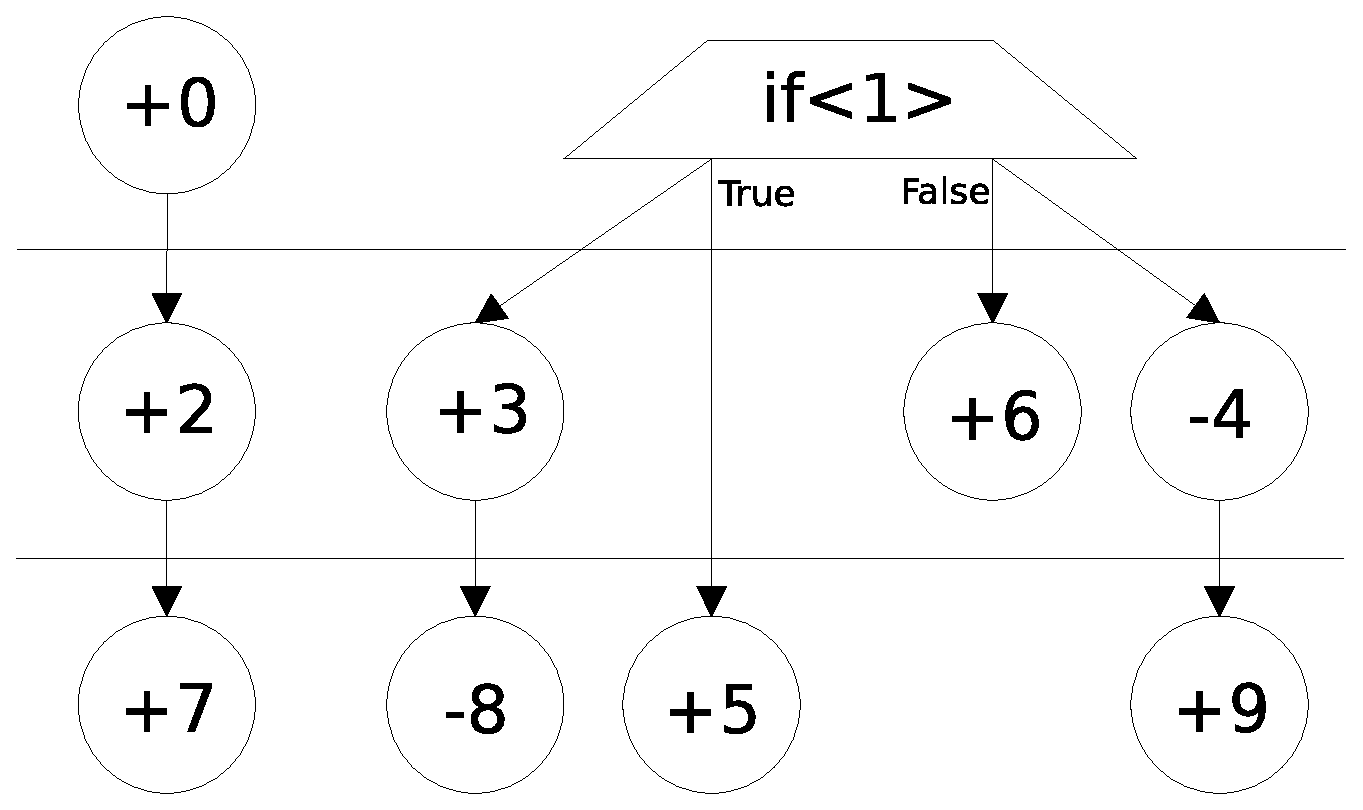
\includegraphics[scale = 0.22]{figures/Diagram8.eps}
}
}
}
\end{center}
\hcaption{Esempio di indecisione nella scelta di un assegnamento in caso di costrutti condizionali}\label{f:ex2}
\label{c:my:var:force}
\end{figure}
Consideriamo l'esempio riportato in figura \ref{f:ex2}: in \ref{f:ex2:a} � riportato un SDG di esempio con un'operazione di tipo salto condizionale; in \ref{f:ex2:b} sono riportate le distribuzioni di probabilit� (l'etichette T ed F indicando se le operazioni fanno parte del ramo \emph{then} o del ramo \emph{else} del costrutto condizionale) e le somme di probabilit�. Applicando l'algoritmo otteniamo una forza nulla per i quattro possibili assegnamenti: quale di questi si deve scegliere? Si potrebbe pensare che la scelta essendo le forze tutte uguali sia indifferente. Provando a compiere due scelte diverse, quindi a calcolare le forze per l'operazione rimanente e a schedularla si ottengono i risultati mostrati in \ref{f:ex2:ca} e \ref{f:ex2:cb}. Se valutiamo i due scheduling, trascurando le unit� funzionali necessarie per sottrazione e costrutto condizionale che sono in numero uguale in entrambi i casi, si pu� notare come nel primo caso siano necessari tre unit� funzionali in grado di eseguire addizioni, nel secondo caso solo due. A questo punto si potrebbe pensare che per compiere la scelta migliore basterebbe, nel caso si presentino pi� forze eguali, considerare altri fattori come l'effettiva occupazione dopo l'assegnazione o introdurre tecniche di look-ahead. 
\begin{figure}
\begin{center}

\subfigure[SDG di esempio]{
\label{f:ex3:a}
\fbox{
\ifthenelse{\boolean{pdf}}
{
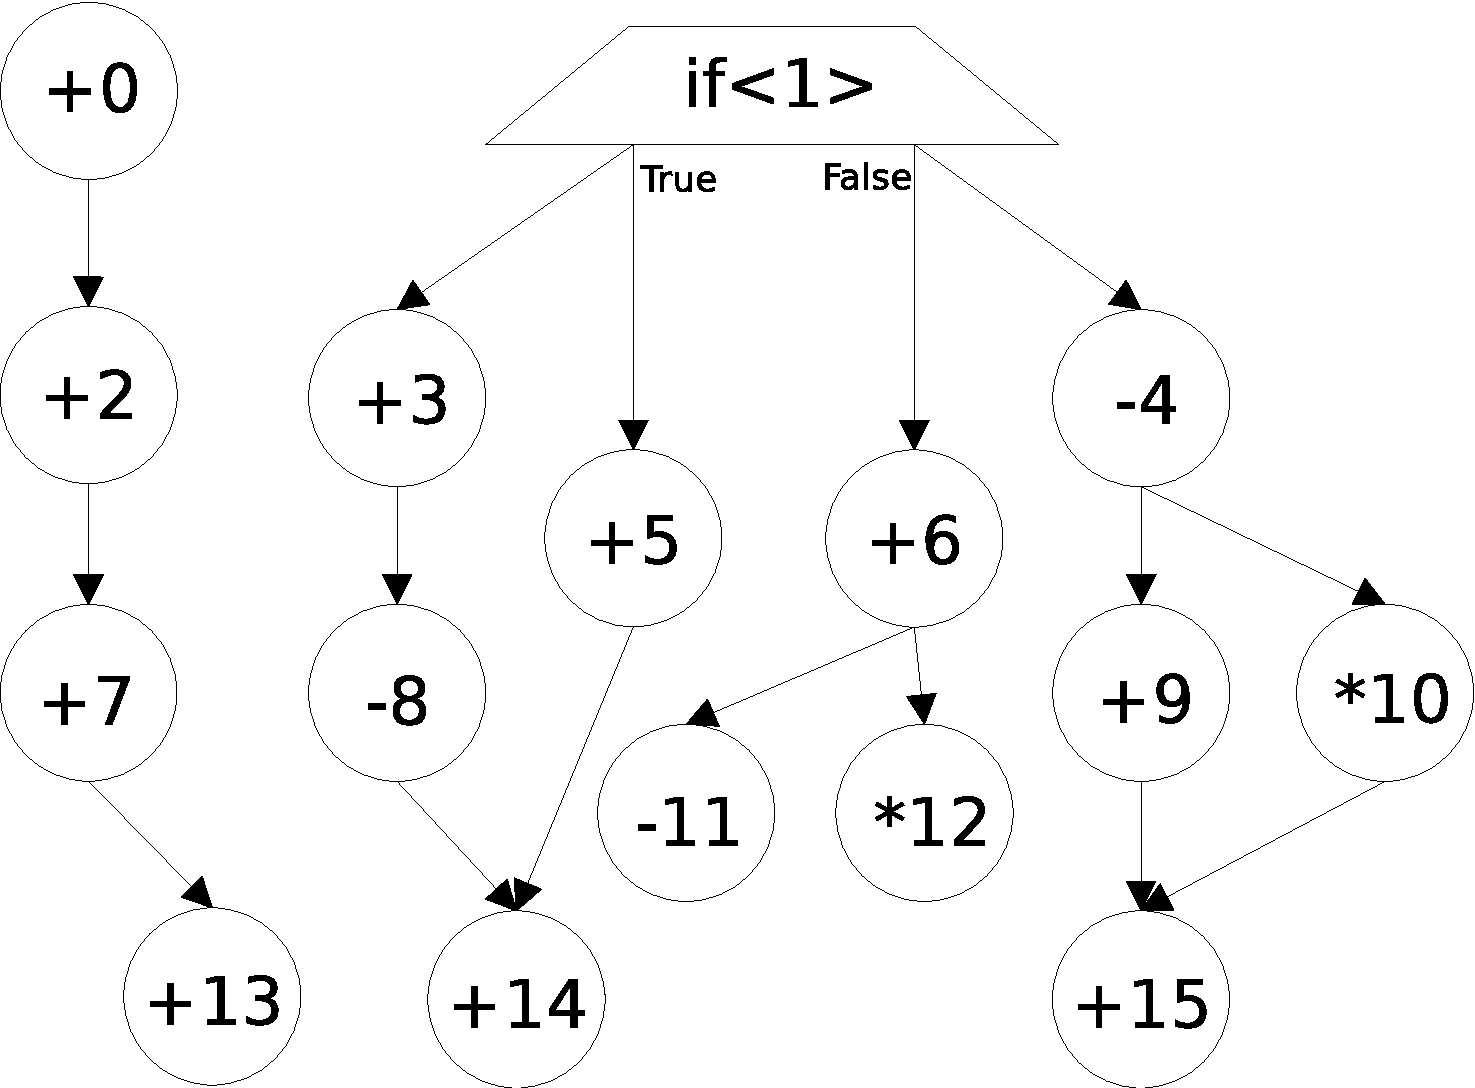
\includegraphics[scale = 0.22]{figures/Diagram9.pdf}
}{
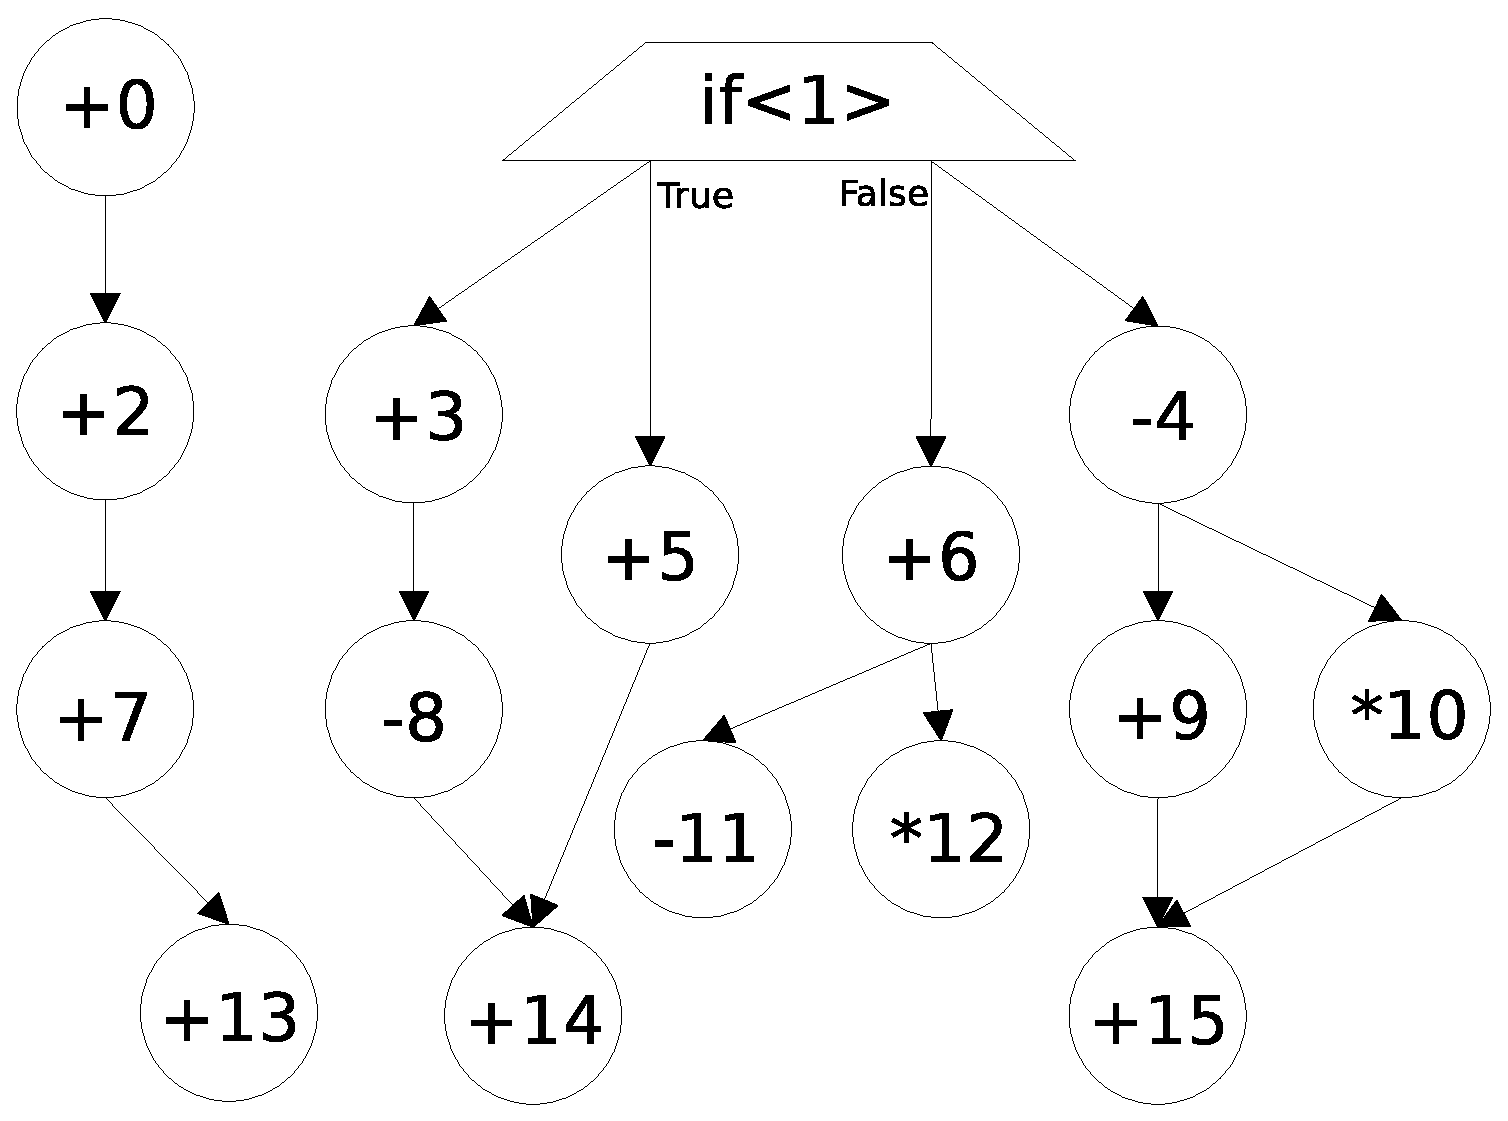
\includegraphics[scale = 0.22]{figures/Diagram9.eps}
}
}
}
\subfigure[Distribuzione di probabilit� e somma di probabilit�]{
\label{f:ex3:b}
\ifthenelse{\boolean{pdf}}
{
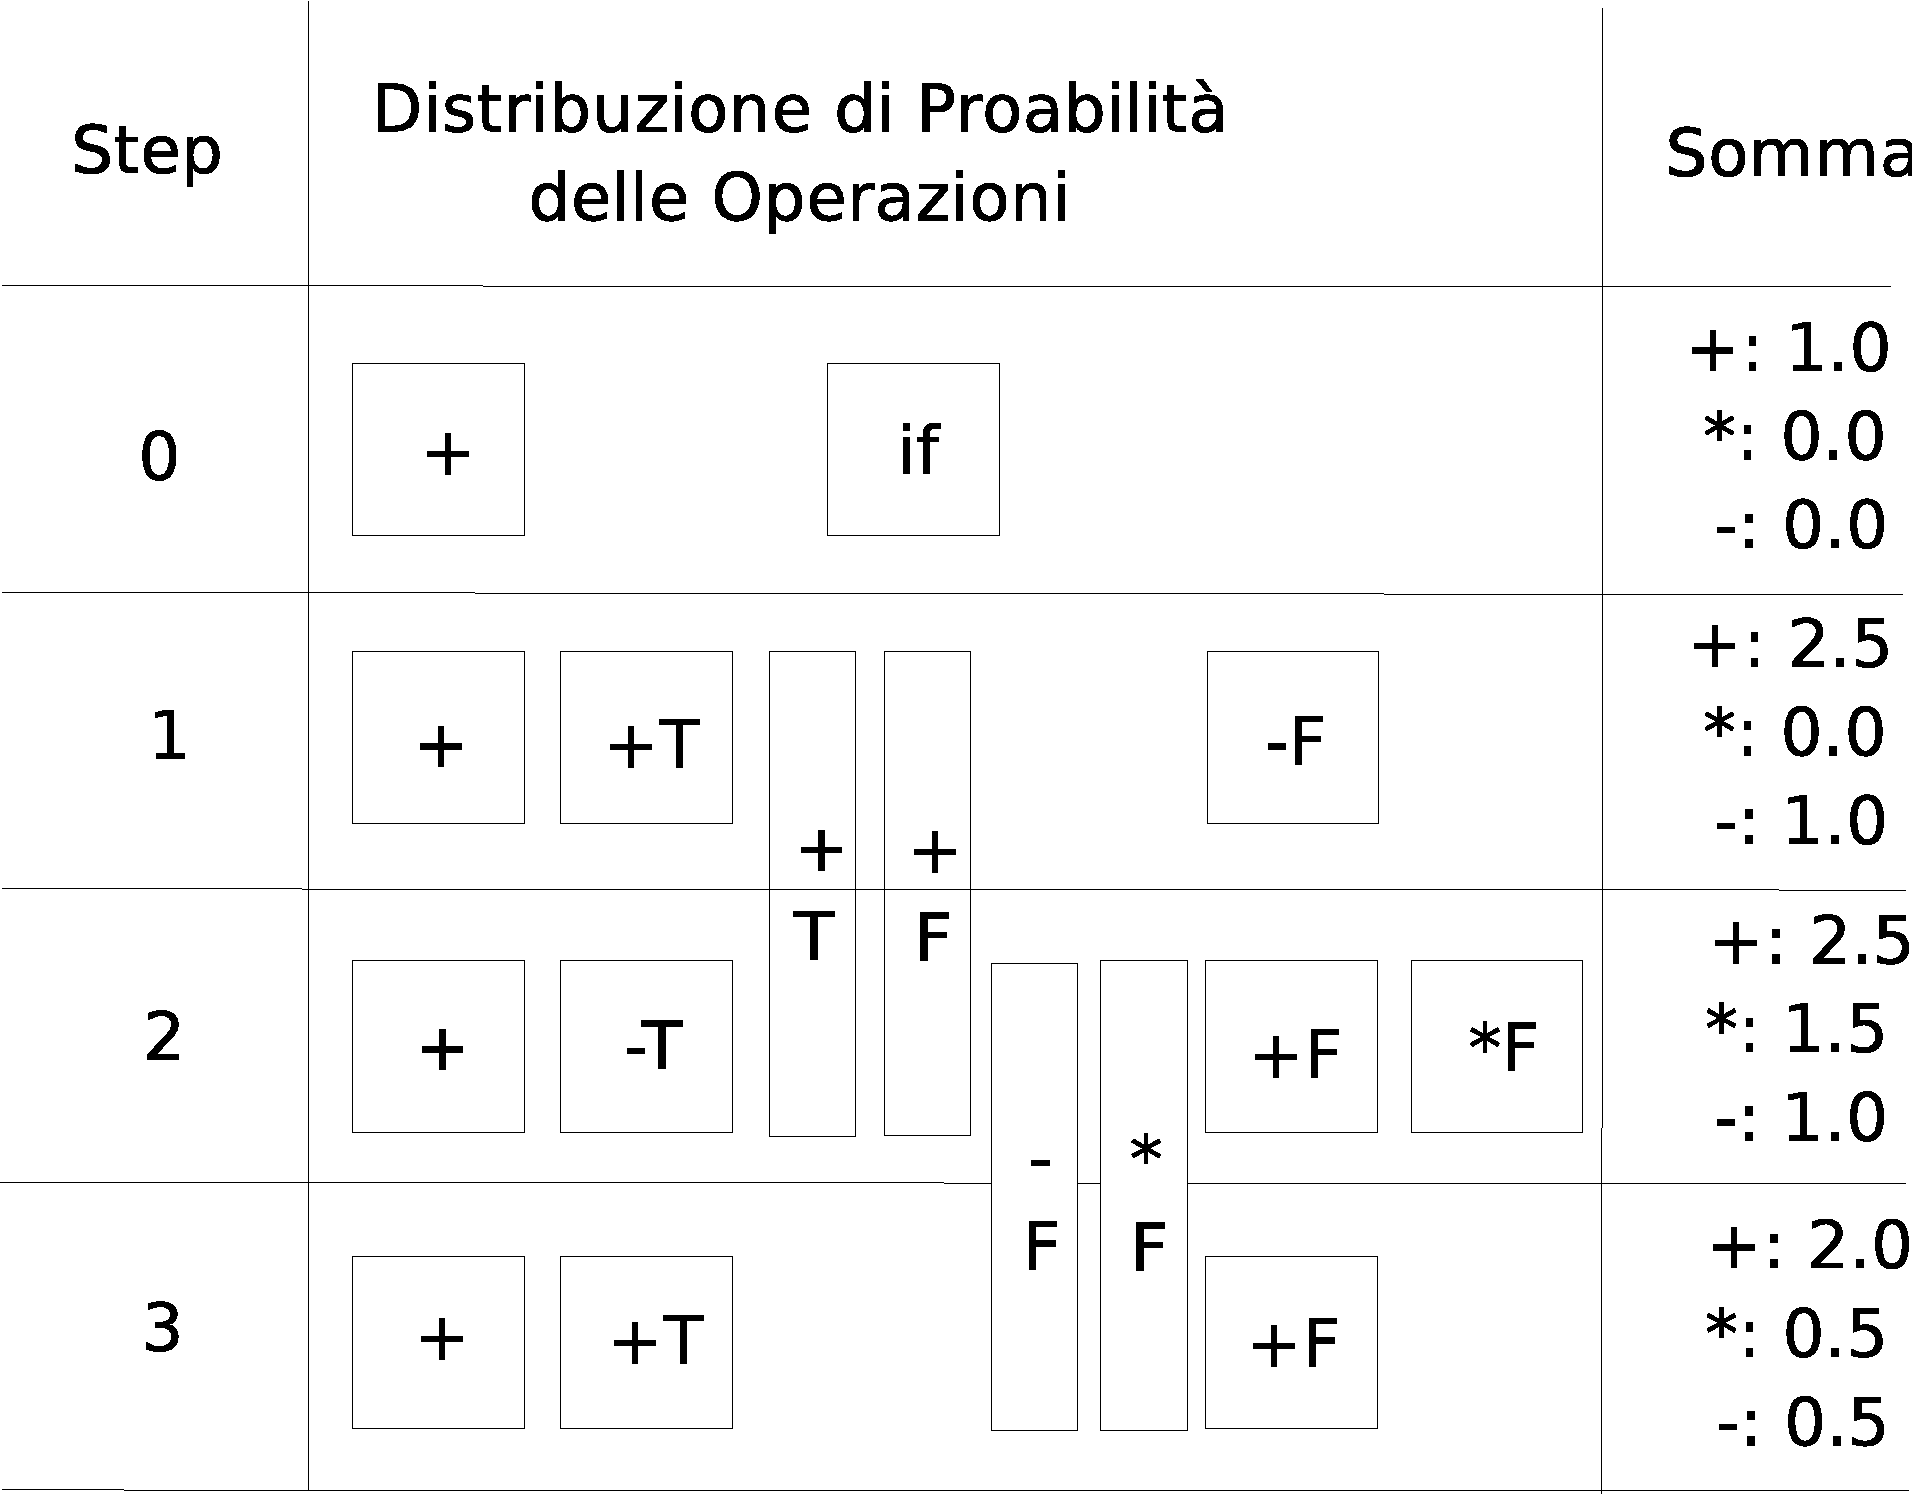
\includegraphics[scale = 0.22]{figures/Diagram10.pdf}
}{
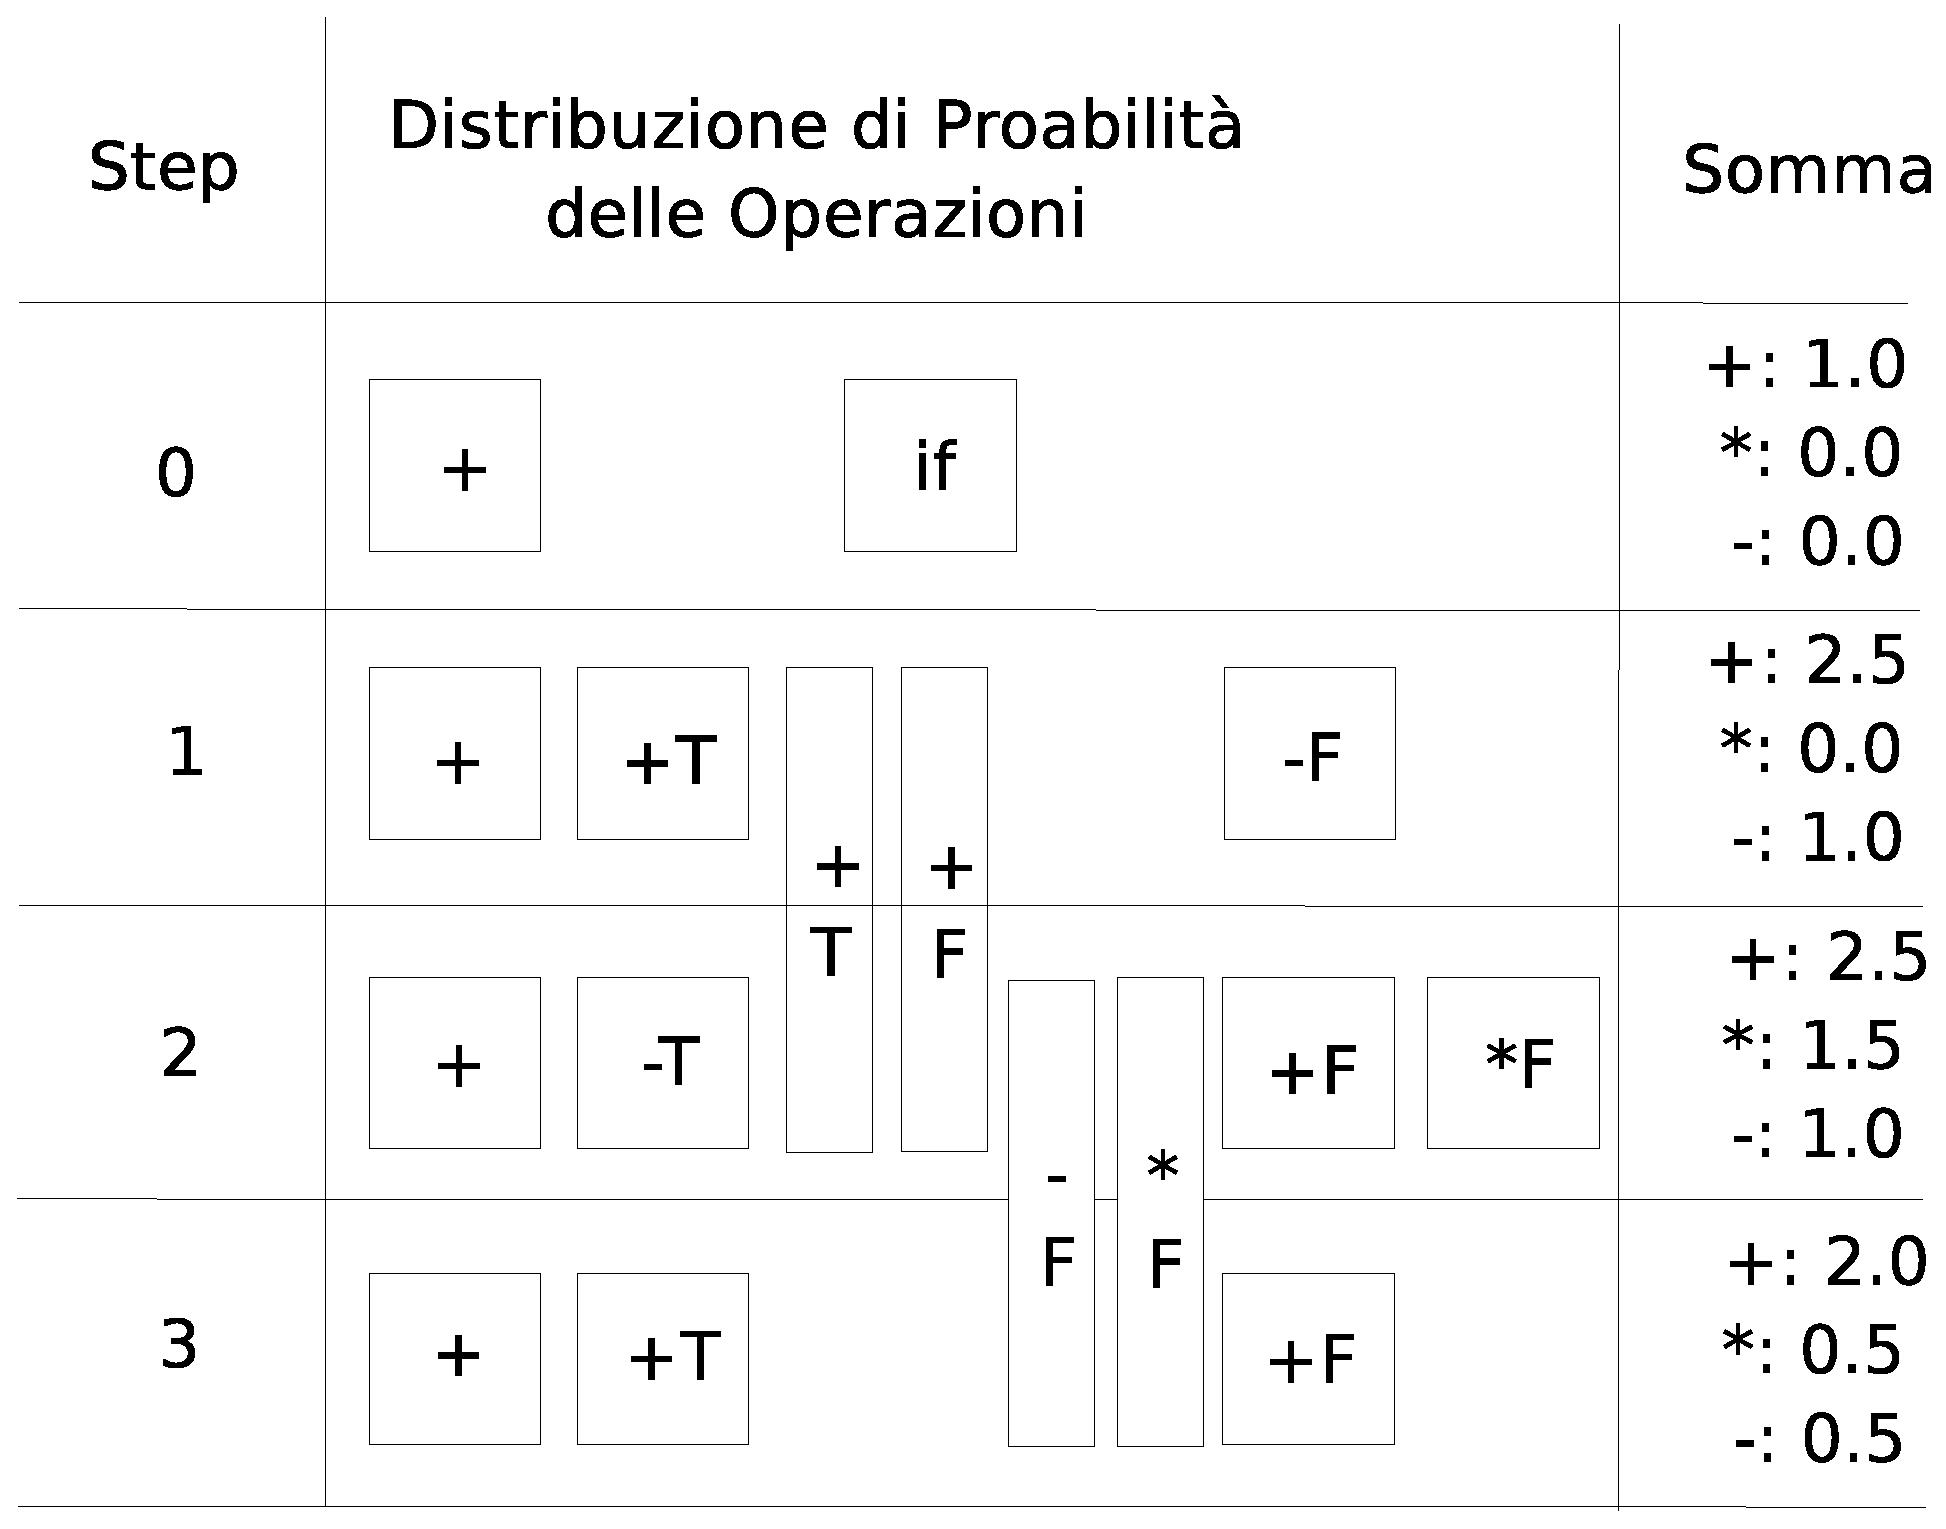
\includegraphics[scale = 0.22]{figures/Diagram10.eps}
}
}
\end{center}
\begin{center}
\subfigure[Tabella delle forze delle operazioni da schedulare \newline SF = self forces \newline OF = predecessors' and successors' forces \newline TF = total forces ]{
\label{f:ex3:tab}
\begin{tabular}{|l|r||r|r|r|}
\hline 
Op & CS & SF & OF & TF \\
\hline
\hline
+5 & 1 & 0.0 & 0.0 & 0.0 \\
\hline
+5 & 2 & 0.0 & 0.0 & 0.0 \\
\hline
+6 & 1 & 0.0 & 0.0 & 0.0 \\
\hline
+6 & 2 & 0.0 & -0.75 & -0.75 \\
\hline
\end{tabular}
\hspace{0.5 cm}
\begin{tabular}{|l|r||r|r|r|}
\hline 
Op & CS & SF & OF & TF \\
\hline
\hline
-11 & 2 & +0.25 & 0.0 & +0.25 \\
\hline
-11 & 3 & -0.25 & 0.0 & -0.25 \\
\hline
*12 & 2 & +0.5 & 0.0 & +0.5 \\
\hline
*12 & 3 & -0.5 & 0.0 & -0.5 \\
\hline	
\end{tabular}
}
\end{center}
\begin{center}
\subfigure[Scheduling prodotto dal Force Directed]{
\label{f:ex3:ca}
\fbox{
\ifthenelse{\boolean{pdf}}
{
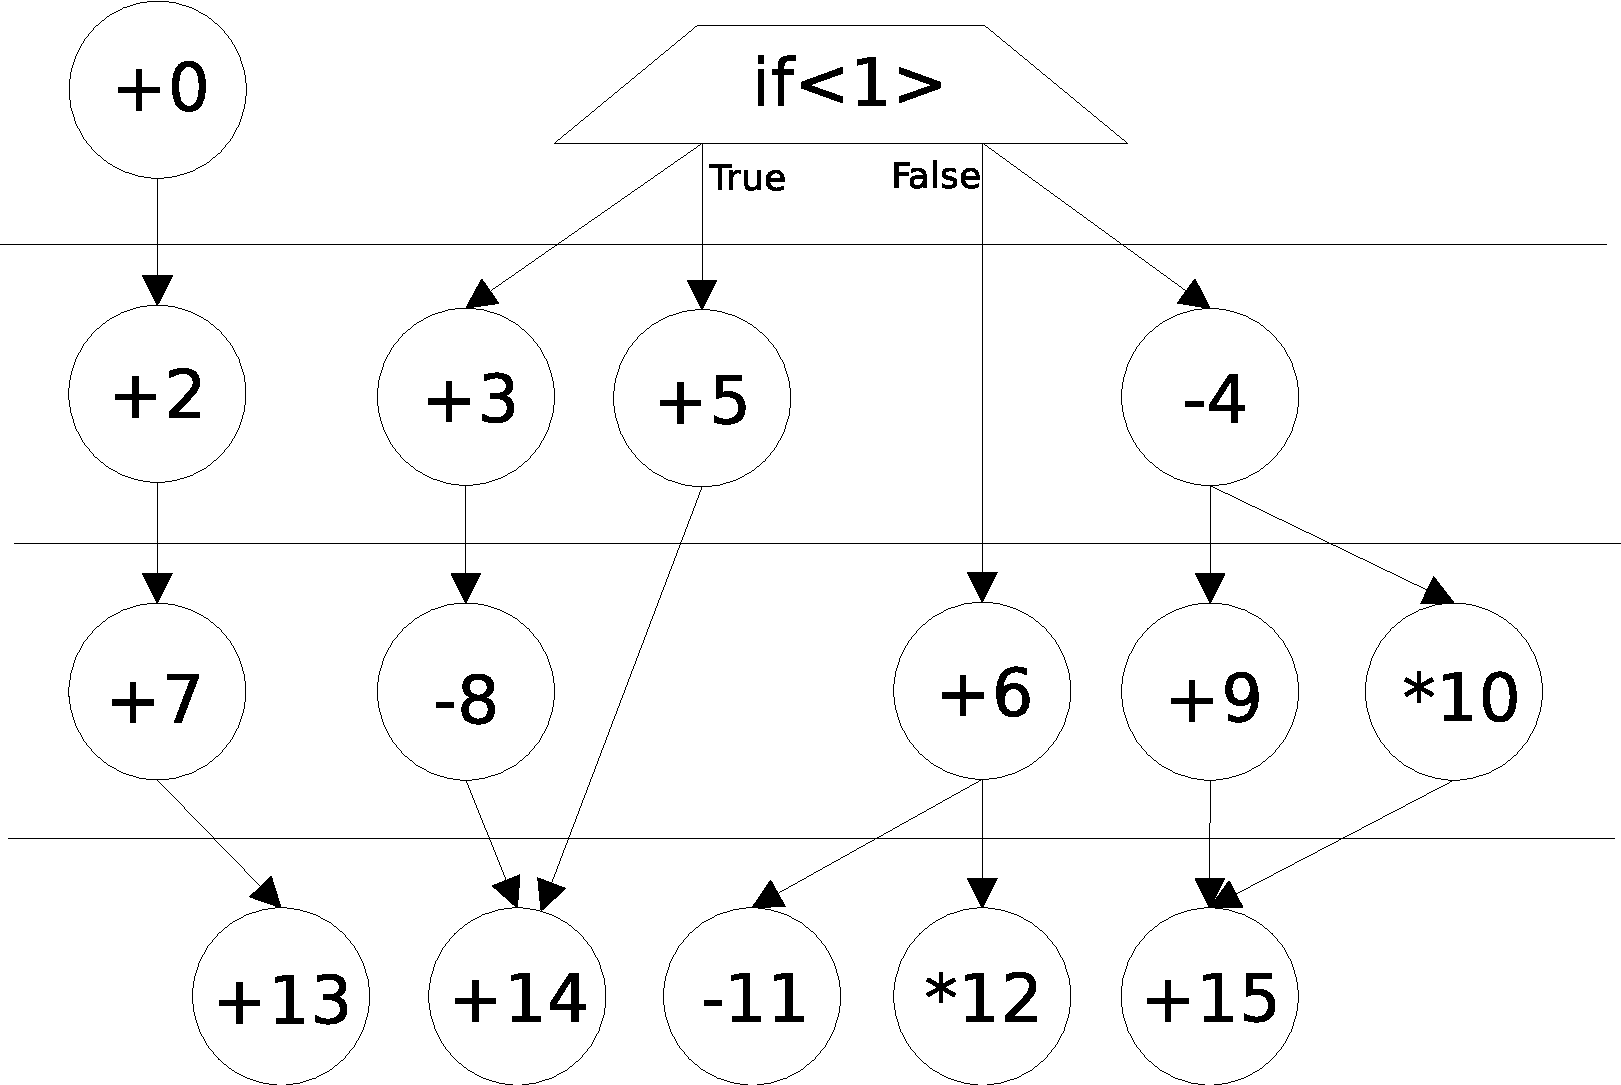
\includegraphics[scale = 0.22]{figures/Diagram11.pdf}
}{
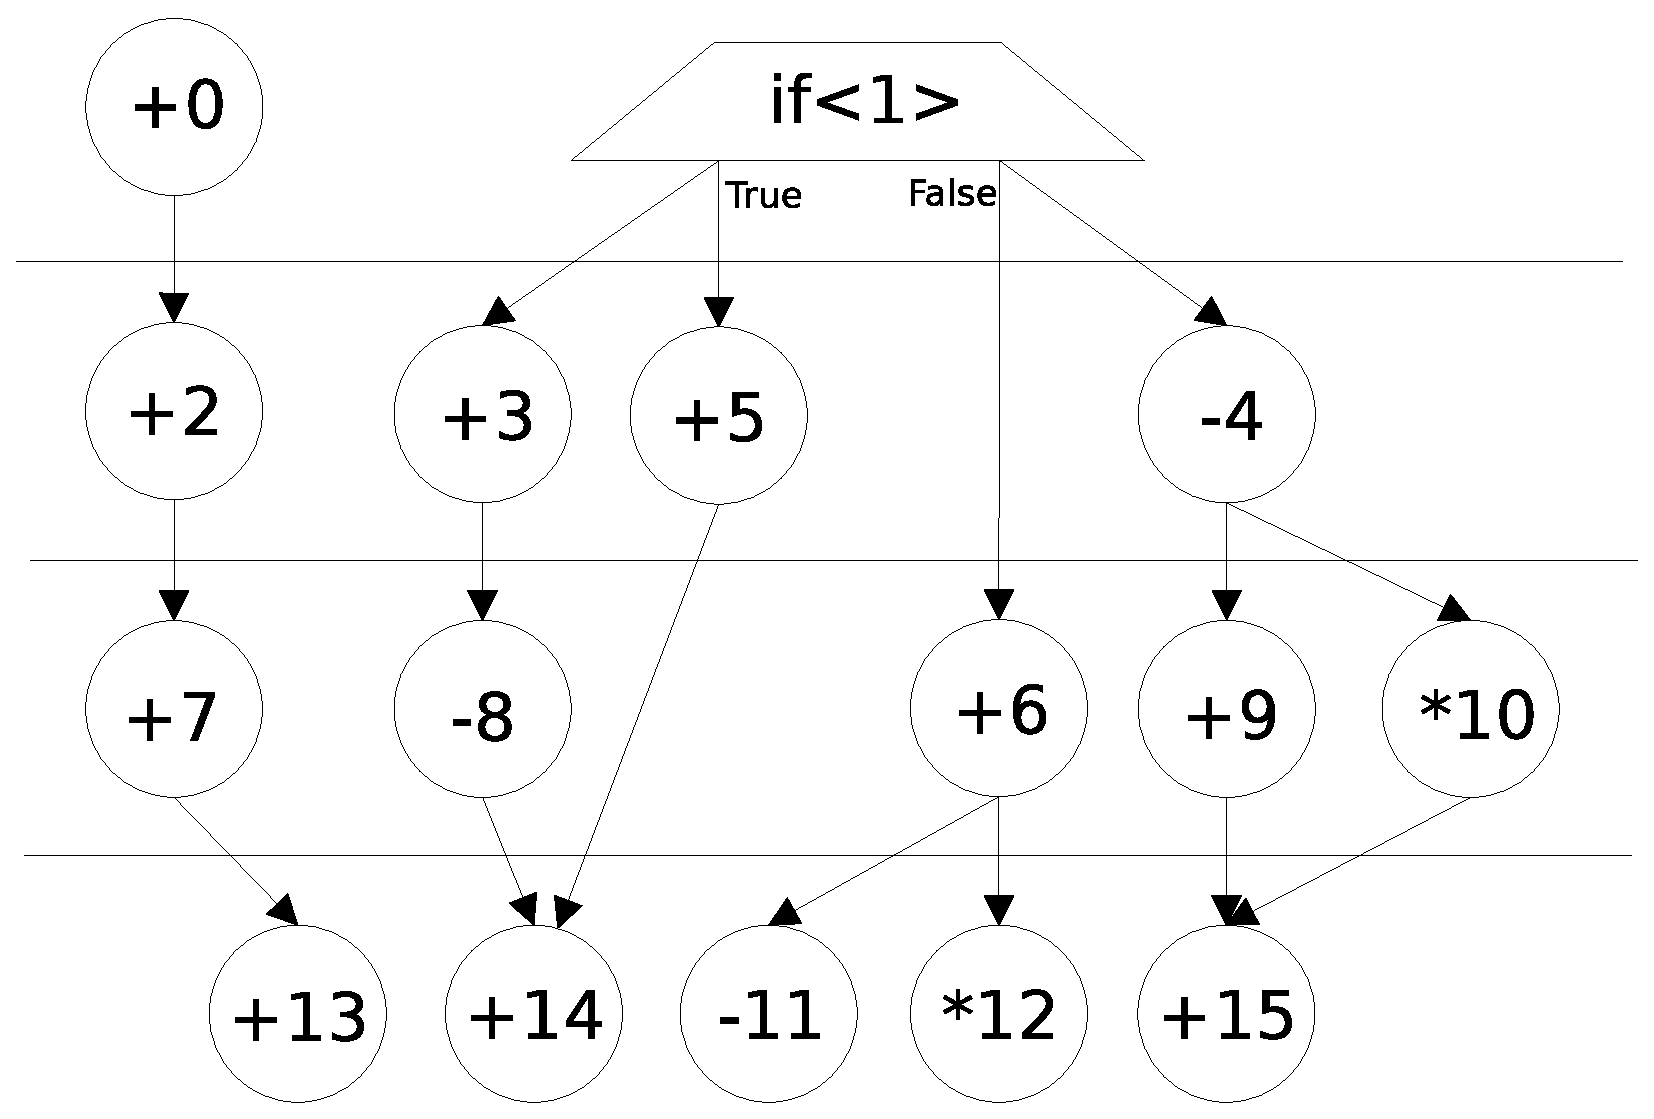
\includegraphics[scale = 0.22]{figures/Diagram11.eps}
}
}
}
\subfigure[Scheduling ottimo]{
\label{f:ex3:cb}
\fbox{
\ifthenelse{\boolean{pdf}}
{
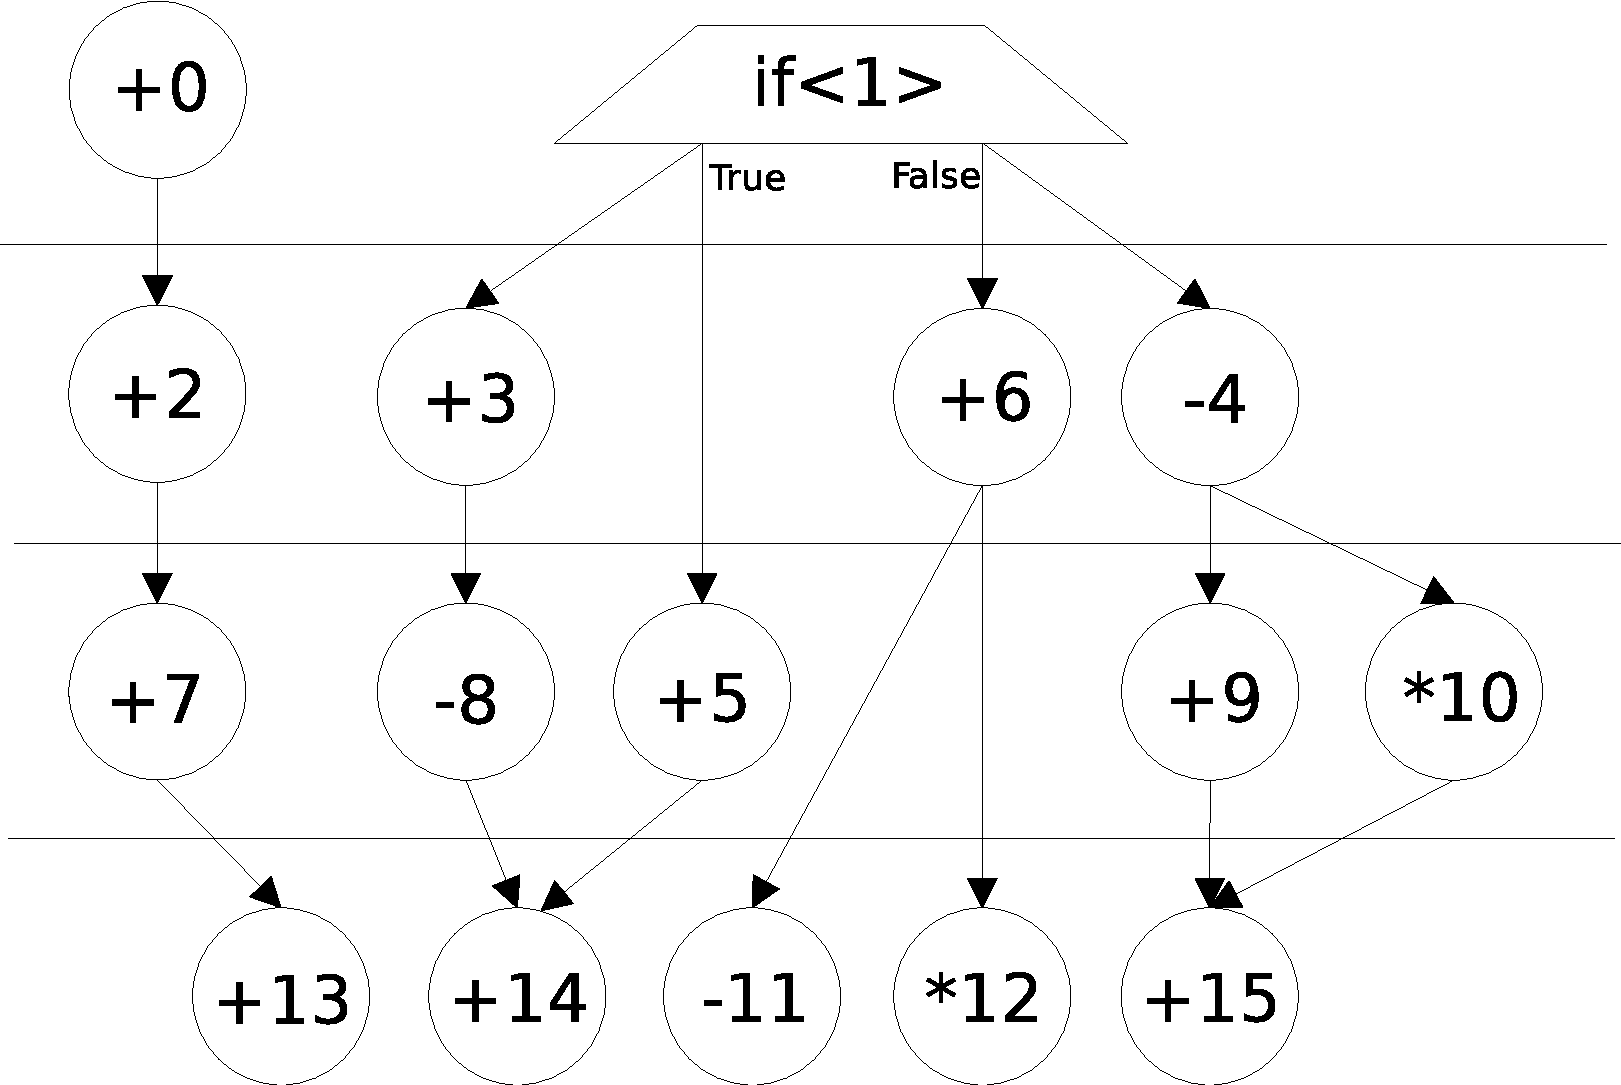
\includegraphics[scale = 0.22]{figures/Diagram12.pdf}
}{
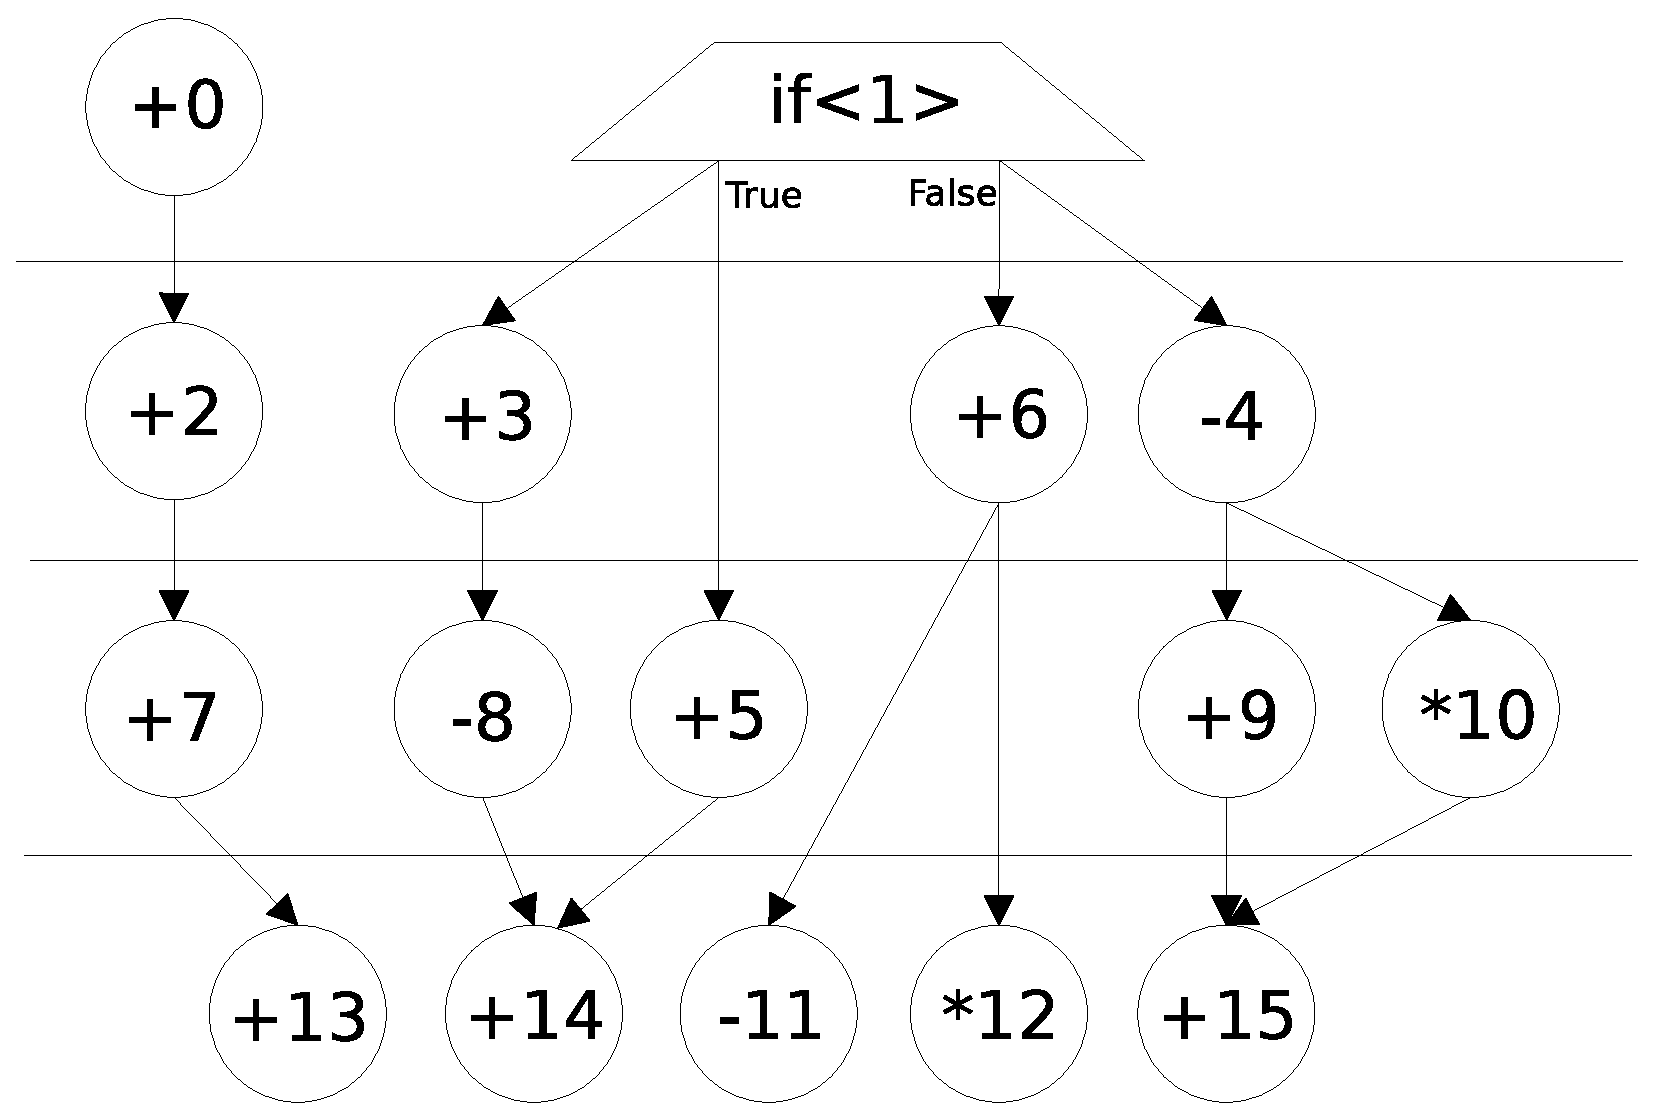
\includegraphics[scale = 0.22]{figures/Diagram12.eps}
}
}
}
\end{center}
\hcaption{Esempio di scelta di assegnamento svantaggiosa in caso di costrutti condizionali}\label{f:ex3}
\end{figure}

A questo punto il problema di scheduling in oggetto viene modificato aggiungendo nuove operazioni come mostrato in \ref{f:ex3:a}. Applicando in questo caso l'algoritmo non si hanno casi di indecisione perch� la scelta che propone di fare l'algoritmo (\ref{f:ex3:tab}) � chiaramente di assegnare l'operazione \emph{+6} al passo di controllo \emph{2}. Il risultato di questa decisione � mostrato in \ref{f:ex3:ca}: tale soluzione utilizza un sottrattore, un moltiplicatore e tre addizionatori. Tuttavia eseguendo lo scheduling manualmente si individua facilmente la soluzione riportata in \ref{f:ex3:cb} che utilizza un sommatore in meno. Alla luce di questo esempio anche la possibilit� di introdurre un raffinamento dell'algoritmo in caso di indecisione appare inutile perch� possono presentarsi situazioni simili in cui la scelta suggerita � unica, ma palesemente svantaggiosa. Introdurre una tecnica di look-ahead completa che venisse utilizzata in tutte le occasioni � stato dimostrato essere troppo penalizzante in \ref{c:ori:longcore:look} (tecniche di look-ahead). Conviene quindi analizzare questo particolare tipo di situazioni e chiedersi perch� l'algoritmo suggerisca scelte penalizzanti.

L'algoritmo tiene conto della presenza di istruzioni in mutua esclusione solo nel calcolo delle somme di probabilit�: quando si tratta di calcolare la forza di un'operazione tuttavia non si considera come � stata calcolata la somma di probabilit�. Quindi il contributo alla forza di un'operazione relativo ad un passo di controllo tiene conto solo della somma di probabilit� stessa e della mobilit� dell'operazione. Questo comporta che l'algoritmo in realt� per calcolare la forza (gli effetti di un assegnamento di un'operazione a un dato passo di controllo non tenga conto del fatto che l'operazione assegnata sia effettivamente in conflitto con quelle gi� presenti o meno. Schedulare in un passo di controllo un'operazione appartenente ad un ramo then di un costrutto di controllo se gi� sono presenti in quel passo di controllo pi� operazioni dello stesso tipo appartenenti al ramo then stesso e nessuna al ramo else porta ad effetti (� richiesta un'ulteriore unit� funzionale di quel tipo per quel passo di controllo) differenti rispetto a schedulare nella stessa situazione un'operazione appartenente al ramo else (non sono richieste ulteriori unit� funzionali per quel passo). Questa sostanziale differenza non � tenuta in alcun conto dalla versione originale dell'algoritmo che cerca quindi di non schedulare contemporaneamente operazioni del ramo then e del ramo else di un costrutto condizionale anche se esse non concorrono ovviamente per l'accesso ad una risorsa essendo in mutua esclusione.

Per ovviare a questa mancanza si � deciso di modificare l'algoritmo originale in un modo che pu� essere definito sostanziale: in particolare si modifica la  formula della forza che ne costituisce il fondamento. La formula originaria � stata infatti modificata sostituendo un termine in questo modo:
\begin{equation}
Force(i) = DG(i)\cdot\overline{x}(i)
\end{equation}
dove 
\begin{description}
\item[Force(i)]  � la forza dello scheduling relativa all'i-esimo passo di controllo;
\item[DG(i)]  � la somma di probabilit� del tipo di unit� funzionale cui � assegnata l'operazione nell'i-esimo passo di controllo;
\item[$\overline{x}$(i)]  � la variazione non della probabilit� dell'operazione nell'i-esima operazione a seguito dello scheduling ma la variazione della somma di probabilit� dovuta all'assegnamento.
\end{description}
Ovviamente la sostituzione evidenziata dell'ultimo termine della formula viene fatta sia in nel calcolo della \emph{self-force}, sia nel calcolo delle \emph{predecessors' and successors' forces}. Nel caso non vi siano costrutti condizionali o nel caso non possano venir schedulate istruzioni in mutua esclusione nel passo di controllo in oggetto il calcolo delle forze risulta uguale a quello classico perch� la variazione della probabilit� dell'operazione coincide con la variazione della somma di probabilit�. La stessa cosa accade in presenza di costrutti condizionali se l'operazione oggetto della modifica di mobilit� non sia in mutua esclusione con alcuna delle operazioni dello stesso tipo schedulabili in quel passo di controllo. Rimane da evidenziare cosa accade nel caso l'operazione di cui si sta calcolando una forza sia in mutua esclusione con qualcun altra dello stesso tipo schedulabile in quel passo di controllo; � bene introdurre prima tre definizioni relative alla somma di  probabilit� prima di analizzare ci� che pu� accadere; ovviamente tutte le definizioni sottintendono che ci si stia riferendo ad un fissato tipo di operazioni:

\begin{itemize}
\item somma di probabilit� \emph{totale}:

la somma di probabilit� classica evidenziata in \ref{c:ori:core:prob};

\item somma di probabilit� \emph{relativa} (ad un ramo: esso pu� essere un ramo then o un ramo else):

la somma di probabilit� ottenuta considerando solo le operazioni che appartengono ad un ramo condizionale;

\item somma di probabilit� \emph{predominante}:

dato un costrutto condizionale e dati i rami che si dipartono da esso, � definita somma di probabilit� predominante il valore maggiore fra le somme di probabilit� relative e ramo predominante il ramo cui appartiene tale forza.
\end{itemize}

Vengono ora evidenziati i tre casi possibili (le somme di probabilit� si riferiscono ovviamente al tipo di unit� funzionale che pu� eseguire l'operazione):
\begin{itemize}
\item l'operazione fa parte del ramo condizionale predominante:

la somma di probabilit� complessiva sar� quindi pari a quella di quel ramo sommata al contributo della parte non condizionata del SDG; si possono quindi distinguere due ulteriori sottocasi:
\begin{itemize}
\item aumento di probabilit� dell'operazione: 

in questo caso l'aumento di probabilit� dell'operazione provoca un eguale aumento della somma di probabilit�, quindi la forza sar� positiva perch� potenzialmente vi � un aumento della richiesta d'uso dell'unit� funzionale e sar� pari a quella calcolata tradizionalmente;

\item diminuzione di probabilit� dell'operazione: 

in questo caso la diminuzione di probabilit� dell'operazione provoca una diminuzione della somma di probabilit�; la diminuzione � pari a quella della probabilt� stessa a meno che essa non faccia diventare un altro ramo quello predominante; in questo caso la diminuzione della somma � pari alla differenza fra le somme di probabilit� originarie relative dei due rami: infatti le risorse necessarie per effettuare lo scheduling in un passo di controllo sono determinate da quello che attualmente � il ramo di controllo dominante (sommato alle probabilit� delle operazioni che non fanno parte di alcun ramo condizionale);
\end{itemize}
\item l'operazione non fa parte del ramo condizionale predominante:
\begin{itemize}
\item aumento di probabilit� dell'operazione:

se l'aumento di probabilit� non trasforma il ramo non dominante in ramo dominante, la variazione della somma di probabilit� � nulla: infatti le risorse allocate per schedulare il ramo dominante basteranno per schedulare il ramo non dominante compreso l'aumento attuale; se l'aumento trasforma il ramo in dominante allora servir� allocare delle risorse suppletive per colmare il gap fra vecchio e nuovo ramo dominante; tale differenza corrisponder� all'aumento della somma di probabilit� e sar� pari alla differenza fra le somme di probabilit� dei due rami dopo l'aumento;

\item diminuzione di probabilit� dell'operazione:

la diminuzione di probabilit�, intervenendo sul ramo non dominante, non varia le risorse da allocare per effettuare lo scheduling, quindi non varia neppure la somma di probabilit�;
\end{itemize}

\item i rami hanno la stessa somma di probabilit� relativa:

\begin{itemize}
\item aumento di probabilit� dell'operazione:

il ramo a cui appartiene l'operazione diventa automaticamente quello dominante, quindi la somma di probabilit� totale deve essere incrementata dell'aumento di probabilit� dell'operazione;

\item diminuzione di probabilit� dell'operazione:

il ramo a cui non appartiene l'operazione diventa automaticamente quello dominante, quindi l'operazione apparter� al ramo non dominante e pertanto la somma di probabilit� totale rimane inalterata.

\end{itemize}

\end{itemize}

Le considerazioni fatte riguardano il caso con un unico costrutto condizionale. Nel caso di pi� strutture condizionali annidate, il ragionamento � simile e va eseguito iterativamente a partire dai costrutto pi� interno.

\subsection{Correzione nel calcolo di \emph{predecessors' and successors' forces}}
\label{c:my:var:corr}
Come mostrato in \ref{c:ori:core:force} (calcolo delle forze) e come verr� ripreso ed esteso in \ref{c:my:var:next} vi sono delle approssimazioni nel calcolo delle \emph{predecessors' and successors' forces}. Modificare l'algoritmo in modo tale che esso tenga conto esattamente degli effetti provocati da un possibile assegnamento risulterebbe controproducente per l'elevata complessit� che esso assumerebbe che non giustificherebbe l'eventuale guadagno nella qualit� dei risultati. L'approssimazione evidenziata produce in generale una sottostima del valore del \emph{predecessors' and predecessors' forces}. Nel caso di forze dal valore positivo l'approssimazione nel calcolo di questa componente della forza non risulta essere particolarmente penalizzante ai fini delle scelte di assegnamento, in quanto la forza totale sar� tendenzialmente comunque positiva e perci� l'assegnamento corrispondente difficilmente sar� selezionato. Nel caso di forze dal valore negativo invece l'approsimazione nel calcolo pu� portare come mostrato nella figura \ref{f:ex} a delle scelte palesemente svantaggiose. Infatti l'approssimazione pu� trasformare in negative forze in realt� positive e pertanto portare a degli assegnamenti che nel caso di un calcolo corretto non verrebbero effettuati.

Per ovviare a questo problema si � scelto di diminuire il peso dei contribuiti alle \emph{predecessors' and successors' forces} qualora essi fossero negativi in modo tale da renderli trascurabili rispetto a quelli positivi. In questo modo non solo si risolve il problema evidenziato ma si fa s� che si scelgano assegnamenti che non solo migliorino in media la distribuzione, ma che provochino il minor numero possibile di aumenti alle somme di probabilit� e quindi all'utilizzo di unit� funzionali. I contributi negativi verranno quindi considerati solo per ordinare assegnamenti che risulterebbero pari considerando le \emph{self-forces} e i contribuiti positivi delle \emph{successors' and predecessors' forces}.

Ci si pu� chiedere se questa modifica nel calcolo delle forze provochi il trascurare degli scheduling che effettivamente avrebbero un grosso contributo negativo da parte delle \emph{predecessors' and successors' forces} e che cio� provocherebbero una generale riduzione della concentrazione dell'uso di unit� funzionali. Tuttavia se un'operazione d� un contributo negativo ad una qualche \emph{predecessors' and successors' forces}, significa che la riduzione corrispondente della mobilit� dar� comunque vita ad una \emph{self-force} negativa in almeno uno dei passi della finestra temporale ristretta da un altro assegnamento. Se tale assegnamento avesse anche una \emph{predecessors' and successors' force} non positiva o comunque non eccessivamente positiva, tale assegnamento verrebbe comunque prima o poi scelto dall'algoritmo. In tale modo vengono comunque applicati gli effetti benefici previsti da quegli scheduling che si temeva di trascurare. Una volta comunque applicati tali assegnamenti si potr� quindi valutare se l'assegnamento, trascurando gli effetti indiretti provocati da esso (cio� i contributi di predecessori e successori), provochi effettivamente un miglioramento nella concentrazione dell'utilizzo delle unit� funzionali e quindi decidere se debba essere comunque eseguito.

Con la modifica evidenziata in pratica si � variata la filosofia della scelta del prossimo scheduling: non pi� cercare l'assegnamento che migliori mediamente la somma di probabilit� relativa al tipo dell'operazione che si assegna e le somme di probabilit� relative ai tipi dei suoi predecessori e dei suoi successori, ma cercare l'assegnamento che migliori la somma relativa all'operazione dell'assegnamento e che non peggiori o peggiori il meno possibile quelle relative allo stesso tipo negli altri passi di controllo e quelle relative agli altri tipi di operazioni coinvolti indirettamente nell'assegnamento. Questa modifica si far� sentire maggiormente nel caso vengano imposti dei vincoli sulle unit� funzionali (\ref{c:my:vincoli}).

\subsection{Scelta del prossimo assegnamento da effettuare}
\label{c:my:var:next}
Nella sua formulazione originale l'algoritmo prevede che ad ogni iterazione venga scelto quale operazione schedulare e in quale passo di controllo sulla base delle forze relative alle coppie <operazione-passo di controllo>. In \ref{c:my:var:priority} � stato proposto un criterio tramite il quale fornire un ordinamento parziale delle operazioni. Questo ordinamento parziale � utilizzato per limitare le possibili candidate ad essere scelte come prossima operazione da schedulare per limitare la complessit� dell'algoritmo e come � stato mostrato esso non incide particolarmente sui risultati ottenuti perch� gli assegnamenti di operazioni appartenenti ad un gruppo hanno poca influenza sulle operazioni degli altri gruppi.

Al contrario all'interno di uno stesso gruppo l'assegnamento di un'operazione incide fortemente sulle altre perch� spesso ne limita le mobilit� restringendo le finestre temporali dei loro possibili assegnamenti o modifica i valori delle somme di probabilit�. E' quindi cruciale l'ordine in cui all'interno del gruppo vengano scelti gli assegnamenti: la versione originale dall'algoritmo prevede di scegliere l'operazione avente forza minore perch� essa provoca in media una riduzione della richiesta di utilizzo delle risorse necessarie. 

Come sottolineato in \ref{c:ori:core:force} (Calcolo delle Forze) tuttavia mentre il calcolo della \emph{self-force} � per cos� dire esatto, quello delle \emph{predecessors' and successors' forces} � in realt� un'approssimazione basata sul principio di sovrapposizione degli effetti e pertanto non tiene conto esattamente di tutti gli effetti. Ampliando le osservazioni che sono state fatte si pu� anche evidenziare come lo scheduling di un'operazione provochi degli effetti non solo nelle operazioni dello stesso tipo schedulabili contemporaneamente (calcolato come \emph{self-forces}) e nei suoi predecessori e successori (calcolato tramite le \emph{predecessors' and successors' forces}), ma anche, seppur in maniera minore ed indiretta nei successori e nei predecessori delle operazioni dello stesso tipo contemporanee all'operazione di cui si sta calcolando la forza. Infatti tendenzialmente queste ultime, se l'assegnamento teorizzato verr� effettuato, avranno meno possibilit� di essere schedulate nello stesso passo di controllo e questo cambiamento si ripercuoter� anche sui loro predecessori e successori. Questa caratteristica che viene giustamente trascurata per non appesantire la complessit� dell'algoritmo, diverr� molto pi� significativa una volta introdotti dei vincoli sulle risorse come mostrato in \ref{c:my:vincoli}. Infatti nel caso si abbiano a disposizione un numero finito di risorse, un assegnamento che utilizzasse l'ultima risorsa disponibile impedirebbe di fatto lo scheduling di ulteriori operazioni dello stesso tipo in quel passo di controllo modificando quindi la mobilit� loro e dei loro predecessori e successori. Queste considerazioni potrebbero far pensare di dare un peso diverso alle due componenti della forza, analogamente a quanto � stato fatto in \ref{c:my:var:corr}. In questo modo per� si perderebbero ulteriori dati che pur se approssimati possono essere significativi. Invece quello che si vuole � sottolineare che i valori delle forze sono delle approssimazioni pi� o meno accurate degli effetti di un assegnamento.

Un'ulteriore considerazione � che operazioni ad elevata mobilit� e di un tipo poco presente in alcuni passi di controllo possono avere un valore di \emph{self-force} uguale in pi� passi di controllo. Per esempio se si considerano un numero elevato di operazioni dello stesso tipo, la prima avente mobilit� da 0 a 4, le altre limitate al passo di controllo 2 e se non sono presenti altre operazioni di quel tipo, la prima operazione avr� \emph{self-force} uguale nei passi di controllo fra 0 e 4, 2 escluso, e tale valore sar� relativamente basso. Questo valore potrebbe far s� che questa operazione sia la prima ad essere schedulata in virt� della \emph{self-force} cos� elevata tale da assorbire eventuali \emph{successors' and predecessors' forces} positive. A quale passo essa verrebbe assegnata dipenderebbe quindi proprio da queste \emph{successors' and predecessors' forces} che per� come si � visto sono approssimate. Tale scelta per� potrebbe essere cruciale perch� potrebbe influenzare tutti i successivi assegnamenti: infatti mano mano che gli assegnamenti vengono effettuati, la mobilit� delle rimanenti operazioni si riduce finch� molte rimangono con una moblit� unitaria e vengono quindi automaticamente assegnate.

\begin{figure}
\begin{center}
\subfigure[DFG di esempio]{
\label{f:ex4:a}
\fbox{
\ifthenelse{\boolean{pdf}}
{
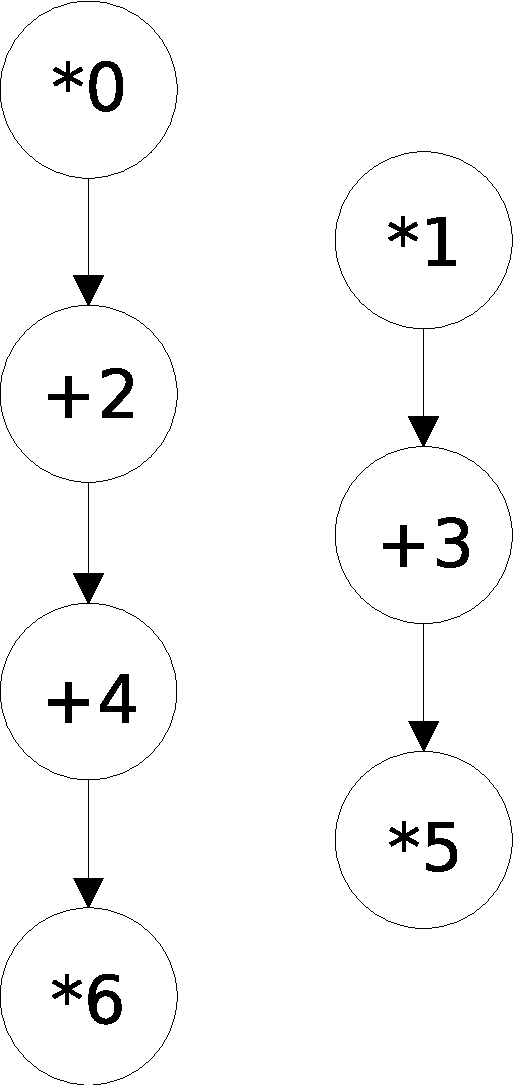
\includegraphics[scale = 0.22]{figures/Diagram13.pdf}
}{
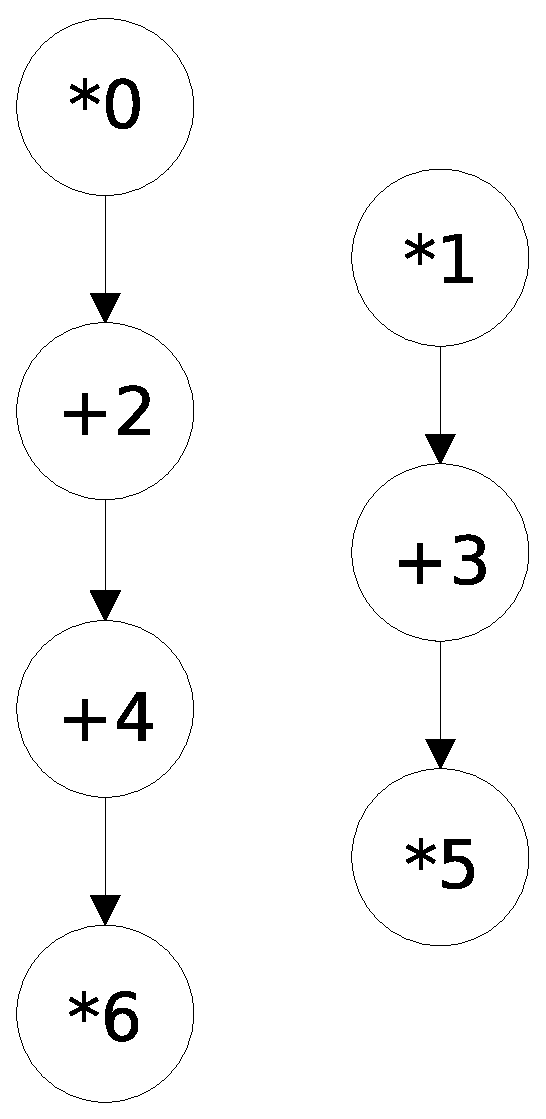
\includegraphics[scale = 0.22]{figures/Diagram13.eps}
}
}
}
\subfigure[Somme di Probabilit�]{
\label{f:ex4:b}
\ifthenelse{\boolean{pdf}}
{
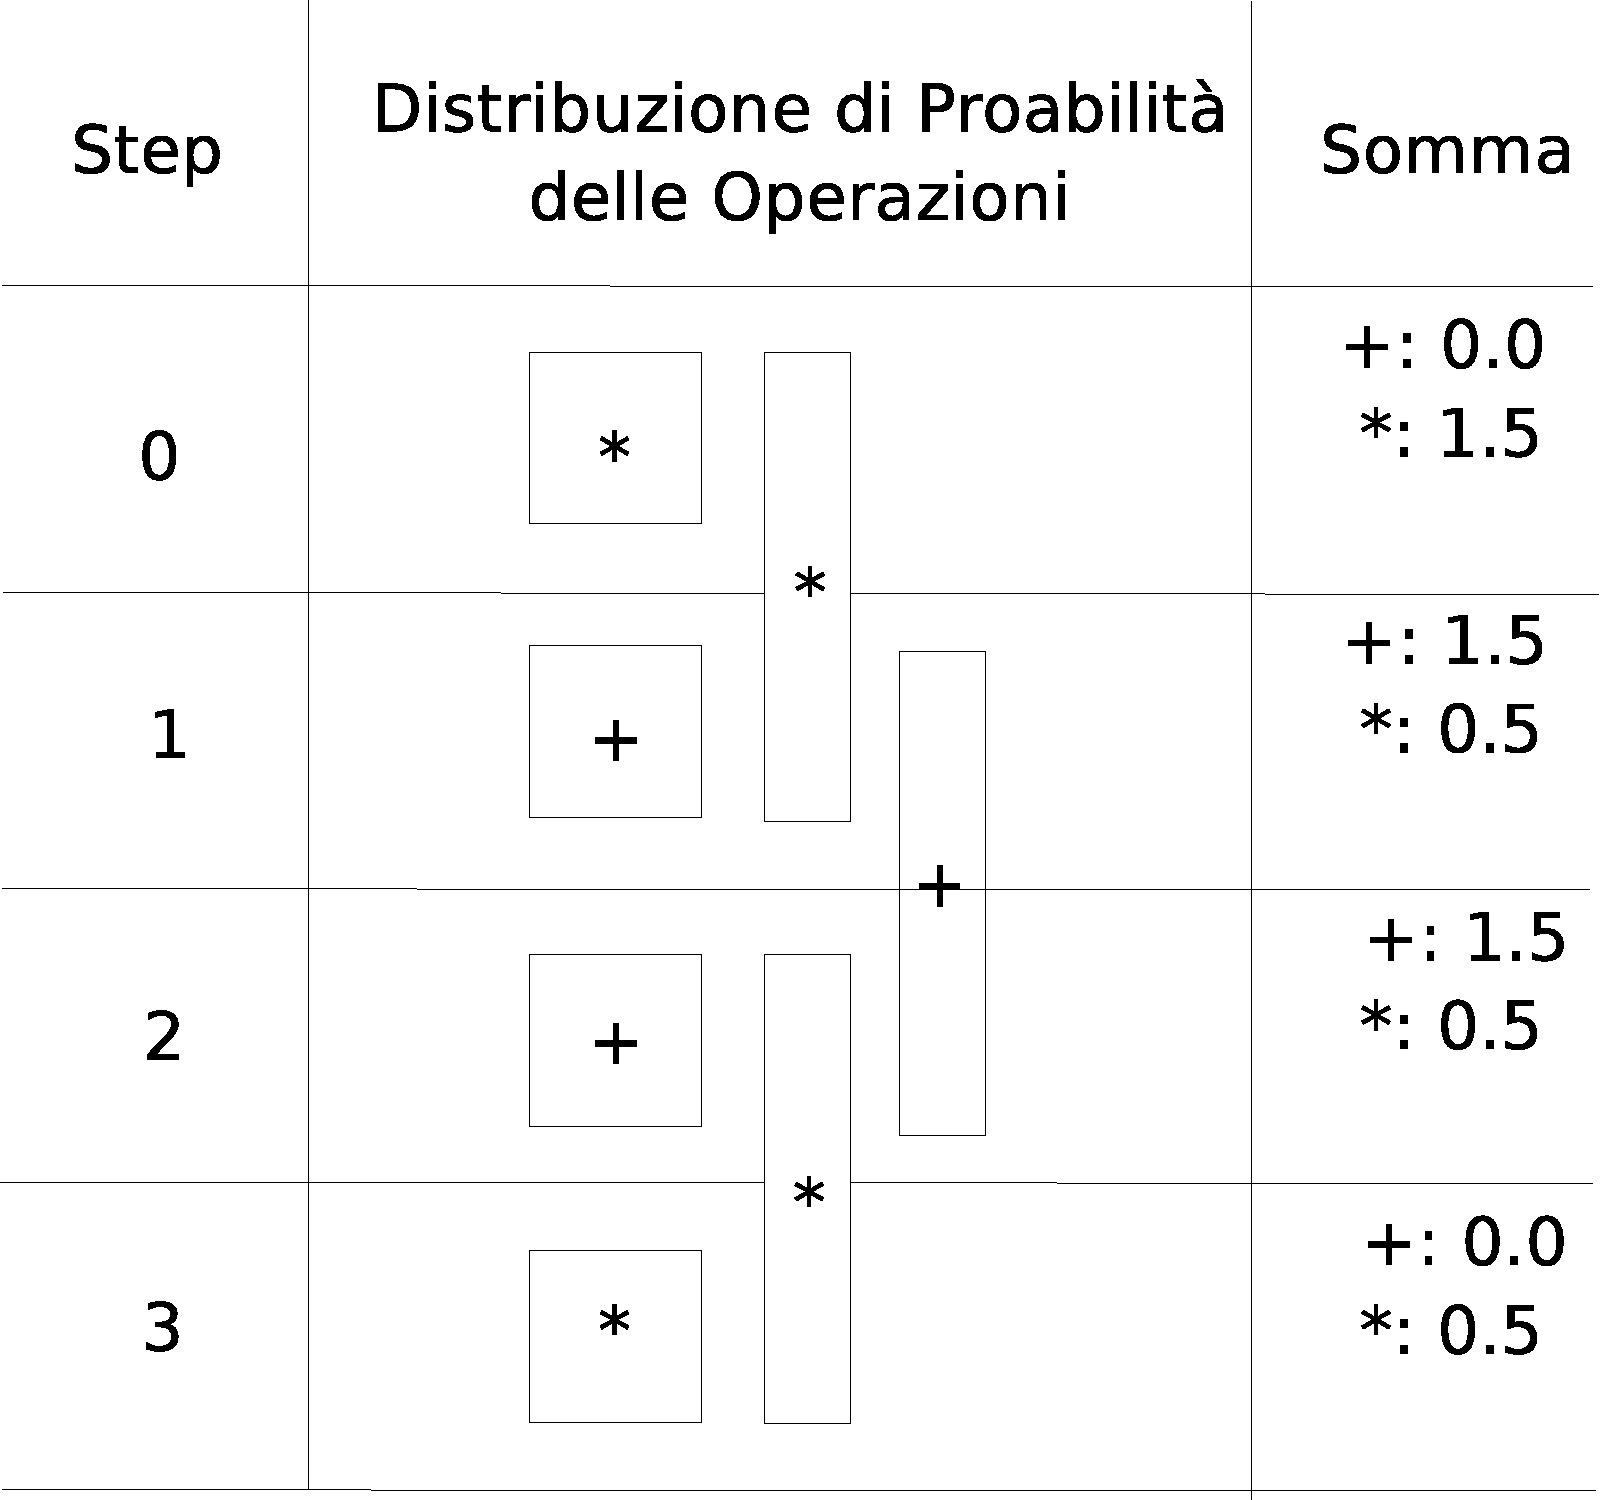
\includegraphics[scale = 0.22]{figures/Diagram14.pdf}
}{
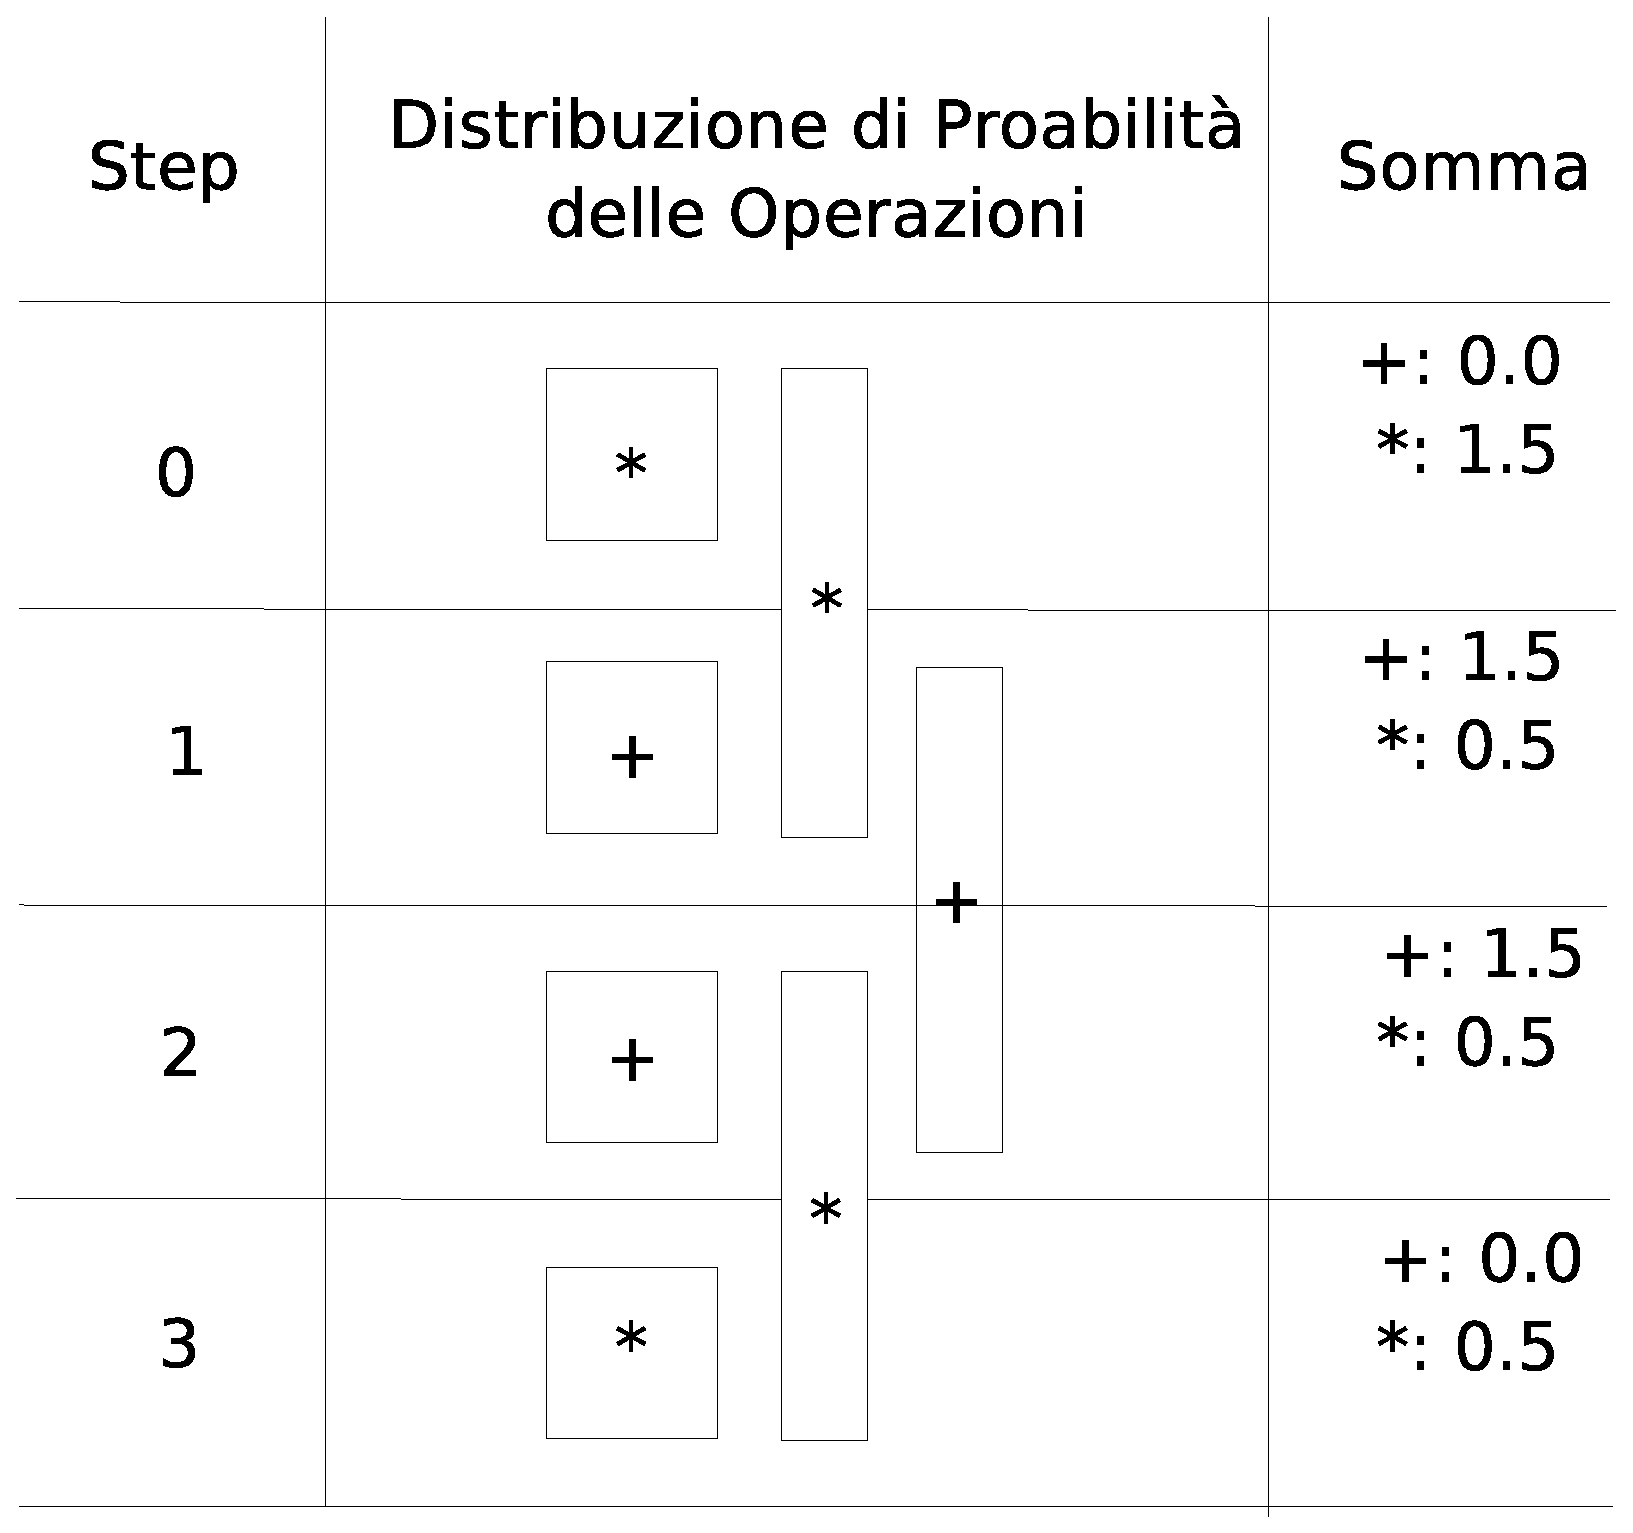
\includegraphics[scale = 0.22]{figures/Diagram14.eps}
}
}
\end{center}
\begin{center}
\subfigure[Tabella delle forze delle operazioni da schedulare \newline SF = self forces \newline OF = predecessors' and successors' forces \newline TF = total forces]{
\label{f:ex4:tab}
\begin{tabular}{|l|r||r|r|r|}
\hline 
Op & CS & SF & OF & TF \\
\hline
\hline
*1 & 0 & +0.5 & -0.5 & 0.0 \\
\hline
*1 & 1 & -0.5 & +0.5 & 0.0 \\
\hline
\textbf{+3} & \textbf{1} & 0.0 & +0.5 & \textbf{+0.5} \\
\hline
\textbf{+3} & \textbf{2} & 0.0 &+ 0.5 & \textbf{+0.5} \\
\hline	
*5 & 2 & -0.5 & +0.5 & 0.0 \\
\hline
*5 & 3 & +0.5 & -0.5 & 0.0 \\
\hline	
\end{tabular}
}

\end{center}
\hcaption[Esempio di Operazione con Forze solo Positive]{Esempio di Operazione (+3) con Forze solo Positive}\label{f:ex4}
\end{figure}

Come mostra l'esempio riportato in figura \ref{f:ex4} esistono problemi con operazioni che sin dalla prima iterazione possono avere forze solo positive. Questa caratteristica comporta che tali operazioni verranno schedulate tendenzialmente per ultime. Ci� pu� comportare che al momento stesso dello scheduling non sia pi� possibile scegliere in quale passo effettuare l'assegnamento a causa della mobilit� ridotta dai precedenti assegnamenti. Tuttavia � facile osservare che queste operazioni possono essere considerate fra le pi� critiche in quanto qualsiasi scelta viene fatta per il loro assegnamento comporta un peggioramento della distribuzione delle operazioni. Verrebbe quindi da pensare che esse dovrebbero avere precedenza nello scheduling. Un modo per fare ci� potrebbe essere quello di scegliere come prossima operazione da schedulare non quella avente forza minore, ma quella avente la forza migliore pi� alta dove con forza migliore di un'operazione intendiamo la forza pi� bassa fra tutte quelle relative agli scheduling di essa possibile. Rimane tuttavia il problema posto inizialmente: le forze come � stato mostrato sono frutto di un calcolo approssimato e quindi alla minor forza, specie se essa si discosta poco dalla seconda pi� bassa, non necessariamente corrisponde una scelta pi� vantaggiosa. Sbagliare nell'assegnare queste operazioni che si � visto essere fra le pi� critiche potrebbe risultare ancora pi� dannoso. 

Alla luce di queste considerazioni si � quindi affrontato il problema da un altro punto di vista: le scelte compiute dell'algoritmo non devono essere tanto nello stabilire quale operazione debba essere schedulata per prima, ma data un'operazione a quale passo di controllo fra quelli possibili essa debba essere assegnata. La decisione che � stata presa � stata quindi quella di riformulare la scelta del prossimo assegnamento seguendo questo procedimento:
\begin{enumerate}
\item si calcola la forza media di ogni operazione ottenuta semplicemente sommando le forze relative a tutti i passi di controllo possibili e dividendo il risultato per il numero stesso dei passi;
\item si calcola lo scostamento della forza minore dell'operazione dalla forza media;
\item si sceglie di schedulare come prossima operazione quella che ha lo scostamento pi� alto; l'assegnamento viene fatto tradizionalmente nel passo di controllo che ha la forza minore.
\end{enumerate}

In questo modo in un certo senso si cerca di prendere la coppia <operazione-passo di controllo> che ha un margine di guadagno maggiore rispetto alle altre coppie formate con la stessa operazione. Questo consente tendenzialmente di rendere trascurabili le approssimazioni nel calcolo delle forze perch� si considera il caso in cui esse hanno meno rilevanza in termini percentuali. Un'altra possibile scelta sarebbe stata quella di selezionare l'operazione che ha maggiore differenza fra la minor forza e la seconda minor forza, ma in questo caso sarebbero state maggiori le possibilit� che le operazioni che sono state definite critiche venissero trascurate almeno inizialmente.

\subsection{Gestione dei cicli}
La gestione dei costrutti iterativi presentata in questo lavoro di tesi differisce da quella proposta da Paulin e Knight. Infatti nell'analisi del SDG l'algoritmo proposto trascura di considerare gli archi di feedback e quindi le relative dipendenze. Questo corrisponde a schedulare una traccia di esecuzione in cui il corpo dei diversi cicli viene eseguito un'unica volta. Lo scheduling delle operazioni appartenenti alle iterazioni successive rispecchier� le distanze temporali relative fra le operazioni appartenenti alla prima iterazione e verr� implicitamente lasciato agli stadi successivi o al controllore stesso. Il modo pi� semplice per assegnare le operazioni delle iterazioni successive � schedularle consecutivamente: l'esecuzione dell'iterazione successiva inizia quando � terminata quella precedente. Per migliorare il tempo di esecuzione complessivo in caso di pi� iterazioni del ciclo � necessario verificare se l'esecuzione di iterazioni successive pu� essere sovrapposta. Questo pu� essere delegato a moduli per l'ottimizzazione dello scheduling dei cicli o al Force Directed stesso tramite la replicazione delle operazioni delle diverse iterazioni come mostrato in \ref{c:ori:longcore:cycle} (Scheduling con cicli nella versione originale). 

Le differenze dell'approccio proposto rispetto a quello originale sono:
\begin{itemize}
\item non � necessario imporre dei vincoli relativi ai singoli cicli nella descrizione comportamentale;
\item il tempo di esecuzione di una singola iterazione � mediamente maggiore a parit� di risorse allocate;
\item � possibile schedulare operazioni non appartenenti al corpo del ciclo contemporaneamente a operazioni ad esso appartenenti.
\end{itemize}

Un modo possibile per forzare un vincolo sulla durata di un'iterazione � manipolare i dati in ingresso all'algoritmo; in particolare � necessario modificare le finestre temporali delle operazioni appartenenti al ciclo in modo tale che la differenza fra l'ASAP dell'operazione corrispondente al costrutto iterativo incrementato del tempo di esecuzione dell'operazione stessa (il primo passo di controllo a cui � possibile assegnare un'operazione appartenente al ciclo) e il maggiore fra i valori ottenuti sommando l'ALAP di un'operazione appartenente al ciclo con il suo tempo di esecuzione (primo passo di controllo in cui sicuramente si pu� assegnare un'operazione appartenente alla successiva iterazione del ciclo) sia pari al tempo imposto dal vincolo.

\subsection{Complessit� dell'Algoritmo modificato}
La complessit� dell'algoritmo pu� essere calcolata come mostrato in \ref{c:ori:core:compl}, metodo che viene qui ripreso brevemente sottolineando l'unica differenza introdotta; con \emph{n} � indicato il numero di operazioni del problema, con \emph{c} il numero di passi di controllo previsto, con \emph{B} il numero di Blocchi Basici e con \emph{b} il numero medio di operazioni presente in un blocco basico (quindi $b \cdot B = n$):
\begin{enumerate}
\item l'algoritmo viene eseguito al massimo per \emph{n} iterazioni;
\item ad ogni iterazione si calcolano le forze relative a massimo \emph{b} operazioni;
\item ogni operazione si pu� schedulare in massimo \emph{c} passi di controllo;
\item ogni operazione ha al massimo \emph{n} fra predecessori e successori, ciascuna schedulabile in massimo \emph{c} passi di controllo.
\end{enumerate}

Il risultato di questo calcolo porta ad una complessit� complessiva di $O(c^2 n^2 b)$ equivalente a $(O\frac{c^2 n^3}{B})$. La riduzione di complessit� rispetto alla versione originale � quindi pari ad un fattore \emph{B}, e quindi nel caso di \emph{SDG} privi di operazioni condizionali il guadagno sar� nullo. L'origine di questa riduzione � dovuta esclusivamente alla modifica mostrata in \ref{c:my:var:priority} (Priorit� delle operazioni).

\section{Estensione all'algoritmo con introduzione dei vincoli sulle risorse}
\label{c:my:vincoli}
In questa sezione verr� illustrato l'estensione dell'Algoritmo con l'introduzione dei vincoli sulle risorse, ma a differenza di quanto suggerito in \cite{fd1} e \cite{fd2} e riassunto in \ref{c:ori:longcore:vincoli} non verranno allentati i vincoli temporali nel fare ci�. Ci si pu� domandare quale sia lo scopo di applicare un algoritmo per minimizzare il numero di risorse quando esse siano gi� state allocate in un numero prefissato. I motivi possono essere molteplici:
\begin{itemize}
\item verificare che non vi siano unit� funzionali che sono inutilizzate e che quindi potrebbero essere eliminate;
\item nel caso i vincoli sulle risorse si riferiscano solo ad alcuni tipi di unit� funzionali, minimizzare il numero di risorse non vincolate;
\item cercare di minimizzare il numero di interconnessioni o il numero di registri;
\item cercare di uniformare l'utilizzo delle unit� funzionali nei vari passi di controllo;
\item fornire non solo un possibile scheduling, ma anche fare il binding di operazioni che possono essere eseguite da pi� tipi di unit� funzionali su uno particolare di questi tipi.
\end{itemize}

L'ultima motivazione anticipa una delle particolarit� dell'estensione all'algoritmo presentata in questa sezione e che verr� precisata in \ref{c:my:vincoli:alloc}.

Le principali modifiche all'algoritmo consistono in una nuova formulazione della distribuzione di probabilit� e conseguentemente delle forze e nell'introduzione del \emph{Backtracking}.

\subsection{Introduzione dei vincoli}
\label{c:my:vincoli:intro}
I vincoli introdotti si riferiscono al limitare il numero di unit� funzionali di un certo tipo allocabili. L'algoritmo non � in grado di rilevare che non esista un possibile scheduling che soddisfi sia il vincolo temporale, sia i vincoli sulle risorse, cio� non � in grado di stabilire se il problema proposto abbia effettivamente soluzione, quindi si devono fornire dei vincoli che permettano almeno uno scheduling ammissibile. E' possibile che i vincoli si riferiscano solo ad alcuni tipi di unit� funzionali, ma per applicare concretamente l'algoritmo proposto � necessario fissare dei vincoli per tutti i tipi di unit� funzionali come verr� mostrato successivamente. Poich� il numero delle unit� funzionali non vincolate sarebbe teoricamente infinito, questo deve essere quantificato in un numero sufficientemente grande: arbitrariamente si � scelto di porlo uguale al numero delle operazioni presenti nel SDG da schedulare. Un suggerimento a come modellizzare il problema � fornito da \ref{c:ori:longcore:arch} (Integrazioni di informazioni relative all'architettura). I pesi da utilizzare non saranno determinati dal costo delle unit� funzionali bens� dal numero di esse disponibili. Per ottenerli basta considerare che il peso presente nel calcolo della forza si riferisca esplicitamente alla somma di probabilit� cio� utilizzare la formula:
\begin{equation}
Force(i) = weighted\_DG(i)\cdot x(i)
\end{equation}
dove \begin{description}
\item[Force(i)] � il contributo alla forza dell'assegnamento relativo all'i-esimo passo di controllo;
\item[weighted\_DG(i)]  � la somma di probabilit� del tipo di unit� funzionale che pu� eseguire l'operazione nell'i-esimo passo di controllo pesata da un opportuno valore;
\item[x(i)] � la variazione della somma di probabilit� nell'i-esimo passo di controllo a seguito dell'assegnamento.
\end{description}

Per ottenere il valore da attribuire ai pesi basta imporre la condizione per tutte le unit� funzionali che la somma di probabilit� pesata sia pari ad uno nel caso la somma di probabilit� corrisponda esattamente al numero di unit� funzionali disponibili di quel particolare tipo. E' proprio per applicare questa uguaglianza che � necessario indicare un numero di unit� funzionali anche per i tipi non vincolati in modo tale da poter pesare anche le somme di probabilit� relative a questi tipi di unit�.

Si considerino due operazioni di tipo diverso, per esempio una somma e una moltiplicazione, e si supponga di avere a disposizione tre sommatori e un moltiplicatore. Si ipotizzi inoltre che le operazioni abbiano la stessa finestra temporale, mobilit� pari a due e che nel primo dei due passi di controllo in cui entrambe possono venir schedulate, le somme di probabilit� pesate relative ad addizionatori e moltiplicatori siano pari ad uno. Se venisse applicata la formula non pesata della forza e si calcolassero le \emph{self-forces} relative al secondo dei due passi di controllo, il contributo ad esse dato dalla riduzione di probabilit� sul primo passo di controllo sarebbe per entrambe -0.5. Si pu� notare che tale riduzione libererebbe per entrambi i tipi di unit� funzionale l'equivalente di 0.5 unit� (si � sempre in un ambito probabilistico, quindi ha senso parlare di frazioni di unit� funzionale) e quindi sembrerebbe coerente che i due contributi alle forze siano pari. Questi valori uguali rispecchiano per� la concezione classica dell'algoritmo. Infatti se si considerano i vincoli sulle unit� funzionali ci si accorge che le due riduzioni di finestra temporale liberano rispettivamente $\frac{1}{6}$ e $\frac{1}{2}$ del totale delle unit� funzionali. Poich� � fondamentale che i vincoli vengano rispettati appare chiaro che la riduzione della seconda operazione dovrebbe dare un contributo diverso e pi� pesante della prima (in questo caso dovrebbe avere un valore minore, perch� le forze migliori sono quelle minori). Per imporre questo comportamento � sufficiente utilizzare non la formula classica per il calcolo della forza, ma la versione proposta in \ref{c:my:var:force} con l'accortezza di pesare la forza non solo pesando il primo termine, cio� la somma di distribuzione di probabilit� ma anche il secondo cio� la differenza di somma di probabilit�. Ovvero:
\begin{equation}
x(i) = \triangle weighted\_DG(i) = \triangle DG(i) \cdot weight(fu)
\end{equation}

dove $weight(fu)$ � il peso relativo all'unit� funzionale considerata. Applicando questa formula si otterranno come contribuiti i valori di -0.16 per l'addizione e di -0.50 per la moltiplicazione.

In generale si pu� notare come l'algoritmo per soddisfare i vincoli relativi alle risorse debba far s� che le somme di probabilit� pesate di tutti i passi di controllo e per tutte le unit� funzionali debbano avere un valore inferiore all'unit� ovvero che sia inferiore ad essa il valore massimo assunto da una somma di probabilit�. Questo obbiettivo rientra appieno nella filosofia iniziale del Force Directed.

Alla luce della formula generale appena introdotta
\begin{equation}
\label{eq:1}
Force(i) = weighted\_DG(i)\cdot \triangle DG(i) \cdot weight(fu)
\end{equation}
� possibile fornire una riformulazione della formula stessa. Tale riformulazione in pratica non cambier� il valore dei termini presenti nella formula e quindi il suo risultato, ma cambier� il loro significato fornendo una nuova interpretazione al problema della minimizzazione delle risorse.

Fino ad ora le distribuzioni di probabilit� descritte nelle sezioni precedenti hanno sempre fatto riferimento alla probabilit� che una certa operazione venisse schedulata in un certo passo di controllo e le somme di probabilit� sono state riferite al numero di operazioni di un certo tipo che probabilmente sarebbero state assegnate a quel determinato passo di controllo. Con questa nuova formulazione al concetto di somma di probabilit� viene sostituito quello di \mbox{\emph{percentuale di occupazione}}. Si associa un valore di questo tipo ad ogni coppia <passo di controllo-tipo di unit� funzionale>: questo valore indicher� la percentuale di unit� funzionali di quel tipo che probabilmente (nello stesso senso inteso nella precedente formulazione; la probabilit� diventa certezza allorch� tutte le operazioni sono state assegnate) sar� occupata in quel passo di controllo. Similmente alla interpretazione originaria si suppone  che se un'operazione ha una mobilit� fissata n, tale operazione occuper� probabilmente una frazione di unit� funzionale pari a 1/n per tutti i passi di controllo della sua finestra temporale. Per ottenere la percentuale di occupazione non di una singola unit� funzionale ma dell'intero blocco � sufficiente dividere il valore ottenuto per il numero stesso delle unit� funzionale di quel particolare tipo. Sommando le occupazioni relative alle singole operazioni ed applicando le considerazioni sui costrutti condizionali presentate in \ref{c:my:var:force} si otterranno facilmente le percentuali di occupazione. A questo punto per ottenere i contributi alle forze sar� sufficiente applicare:
\begin{equation}
\label{eq:2}
Force(i) = \%occ(i,F)\cdot \triangle \%occ(i,F)
\end{equation}
dove 
\begin{description}
\item[Force(i)] � il contributo alla forza dell'assegnamento relativo all'i-esimo passo di controllo;
\item[\%occ(i,F)] � la percentuale di occupazione del tipo di unit� funzionale \emph{F} in quel passo di controllo;
\item[$\triangle$ \%occ(i,F)] � la variazione di occupazione a seguito dello scheduling.
\end{description}
Si pu� facilmente dimostrare che \eqref{eq:1} e \eqref{eq:2} sono equivalenti cio� che il contributo alla forza calcolato � identico. Per dimostrare ci� vengono introdotti alcuni nuovi simboli:
\begin{description}
\item[o] una generica operazione di un tipo fissato eseguibile dalla risorsa \emph{F} e schedulabile in un passo di controllo \emph{i};
\item[prob(o,i)] � la probabilit� che l'operazione \emph{o} venga  schedulata nel passo di controllo \emph{i};
\item[occ(o,i,F)] � la percentuale di occupazione di unit� funzionali di tipo \emph{F} da parte dell'operazione \emph{o} nel passo di controllo \emph{i};
\item[fu(F)] � il numero di unit� funzionali di tipo \emph{F}.
\end{description}
Alcune premesse:


\begin{align}
\frac{1}{mobilita'(o)} & = \frac{1}{mobilita'(o)} \notag \\
\notag \intertext{da questa identit� segue}\\
prob(o,i) & = fu(F) \cdot \frac{1}{mobilita'(o)\cdot fu(F)} \notag \\
\notag \\
prob(o,i) & = fu(F) \cdot occ(o,i,F) \notag \\
\notag \\
\sum_o prob(o,i,F) & = fu(F) \sum_o occ(o,i,F) \notag \\
\notag \\
DG(i) & = fu(F) \cdot \%occ(i,F) \notag \\
\notag \\
\label{eq:3}\frac{DG(i)}{fu(F)} & = \%occ(i,F) 
\end{align}

e per come sono stati ricavati i pesi:
\begin{equation}
\label{eq:4}weight(F) = \frac{1}{fu(F)}
\end{equation}

Si pu� quindi dimostrare che:
\begin{align}
\label{eq:5}
\%occ(i,F)\cdot \triangle \%occ(i,F) & = Force(i) = weighted\_DG(i)\cdot \triangle DG(i) \cdot weight(F)  \notag \\
\%occ(i,F)\cdot \triangle \%occ(i,F) & = Force(i) = DG(i) \cdot weight(F)\cdot \triangle DG(i) \cdot weight(F) \notag \\
\intertext{applicando la sostituzione evidenziata nell'uguaglianza \eqref{eq:4} si ottiene}
\%occ(i,F)\cdot \triangle \%occ(i,F) & = Force(i) = DG(i) \cdot \frac{1}{fu(F)} \cdot \triangle DG(i) \cdot \frac{1}{fu(F)}  \notag \\
\intertext{quindi applicando l'uguaglianza \eqref{eq:3} si ottiene}
\frac{DG(i)}{fu(F)}\cdot \triangle \frac{DG(i)}{fu(F)} & = Force(i) = \frac{DG(i) \cdot \triangle DG(i)}{(fu(F))^2} \notag \\
\intertext{e poich� fu(F) � di fatto una costante si ottiene l'uguaglianza che dimostra l'equivalenza formule per il calcolo dei contributi delle forze e quindi si dimostra l'equivalenza delle due formulazioni del problema}
\frac{DG(i) \cdot \triangle DG(i)}{(fu(F))^2} & = Force(i) = \frac{DG(i) \cdot \triangle DG(i)}{(fu(F))^2}
\end{align}

\subsection{Introduzione del binding su un tipo di unit� funzionale}
\label{c:my:vincoli:alloc}
Nella formulazione stessa del \emph{force Directed scheduling} � implicito che oltre ad eseguire uno scheduling l'algoritmo effettua anche un'allocazione delle unit� funzionali necessarie ad eseguire lo scheduling stesso. Come si � visto in \ref{c:my:vincoli} nelle motivazioni addotte per introdurre i vincoli tecnologici nell'algoritmo, i vincoli pi� o meno parziali in effetti non limitano la funzione di allocazione dell'algoritmo stesso. Per quanto riguarda il binding finora non � stato considerato nella descrizione dell'algoritmo in quanto quest'ultimo non fa differenza fra le singole istanze di uno stesso tipo di unit� funzionale.

I vincoli tecnologici introdotti per� potrebbero prevedere l'esistenza di pi� tipi di unit� funzionali che possano eseguire uno stesso tipo di operazione. Solitamente tali tipi di unit� funzionali si differenziano per qualche parametro che influisce sulle metriche complessive, come ad esempio il tempo di esecuzione o la potenza dissipata nell'eseguire l'operazione. Nella formulazione originaria dell'algoritmo non essendo contemplati limitazioni al numero di unit� funzionali, l'esistenza di pi� unit� funzionali che possono eseguire lo stesso tipo di operazione non complica il problema dello scheduling. Infatti baster� selezionare fra i tipi di unit� funzionali quello che risulter� migliore secondo una certa metrica ed assegnare ad esso le operazioni in oggetto. Se si ipotizza per� di avere i vincoli sul numero di unit� funzionali allocabili questa semplificazione non � pi� possibile perch� potrebbero essere necessari per ottenere uno scheduling valido entrambi i tipi di unit� funzionale. Ci si pu� chiedere perch� si introducano in un'architettura almeno due tipi diversi di unit� che eseguano la stessa operazione. Le motivazioni possono essere diverse:
\begin{itemize}
\item uno dei due tipi di unit� viene allocato perch� consente di eseguire anche altre operazioni: per esempio sommatori e ALU;
\item uno dei due tipi di unit� ha prestazioni (tempo di esecuzione) migliori dell'altra, ma costi pi� elevati; si � scelto quindi nello stabilire l'architettura un compromesso fra l'utilizzo esclusivo di un tipo di unit� funzionale e fra l'utilizzo esclusivo dell'altro tipo.
\end{itemize}

Questa possibilit� pone un nuovo problema: quale criterio utilizzare per assegnare un'operazione ad una unit� funzionale di un tipo piuttosto che ad una di un altro qualora questa sia eseguibile da entrambi. Una prima ipotesi � quella di utilizzare un altro algoritmo per prendere queste decisioni; una volta ottenuto i risultati basterebbe eseguire il Force Directed costruendo le somme di probabilit� o l'occupazione delle unit� funzionali sulla base degli assegnamenti <operazione-tipo di unit� funzionale> gi� eseguiti. Questi assegnamenti in realt� influenzano direttamente lo scheduling perch� i tempi di esecuzione di un'operazione potrebbero dipendere dal tipo di unit� funzionale su cui essa viene eseguita. Questa diversit� si ripercuote sulla mobilit� dell'operazione e quindi indirettamente anche sulla mobilit� di successori e predecessori. Sulla base di queste considerazioni si � scelto di incorporare all'interno dell'algoritmo il binding di un'operazione ad un tipo di unit� funzionale (non alla specifica istanza dell'unit� funzionale).

Per modellizzare questo problema, viene esteso il concetto di forza: viene infatti calcolata una forza per ogni assegnamento possibile che, sulla base di quanto esposto, sar� costituito non dalla coppia <operazione-passo di controllo> bens� dalla terna <operazione-passo di controllo-tipo di unit� funzionale>. 
Di fatto vi sar� differenza solo per le operazioni che possono essere eseguite da pi� tipi di unit�. Per le altre operazioni esister� un'unica forza per la coppia <operazione-passo di controllo> e il binding sar� automaticamente fatto con l'unico tipo di unit� funzionale possibile. Il calcolo della forza viene fatto utilizzando la formula gi� proposta in \ref{c:my:vincoli:intro}:
\begin{equation}
\label{eq:6}
Force(i) = \%occ(i,f)\cdot \triangle \%occ(i,f)
\end{equation}
cio� utilizzando non la somma di probabilit� bens� la percentuale di occupazione di quel tipo di unit� funzionale.

Come verr� mostrato tuttavia tale formula nel caso in oggetto non costituisce una reinterpretazione della formula originale con l'introduzione dei pesi poich� le \emph{\%occ} verranno calcolate in modo diverso, quindi l'uguaglianza \eqref{eq:5} non sar� valida in questo caso. Per determinare le $\%occ(i)$ � necessario calcolare i contributi relativi alle singoli operazioni. Essi dipendono dalla probabilit� che l'operazione venga schedulata in quel passo di controllo su quel tipo di unit� funzionale. In questo caso la funzione di distribuzione della probabilit� sar� bivariata: si deve assegnare una probabilit� per ogni coppia <tipo di unit� funzionale-passo di controllo>. Tale funzione sar� ovviamente nulla per le coppie che non consentono un assegnamento valido. Una caratteristica che tale funzione deve necessariamente avere �:
\begin{equation}
\sum_f f(c,f,o) = \frac{1}{mobilita'(o)}
\end{equation}
dove \emph{c} � un generico passo di controllo appartenente alla finestra temporale dell'operazione, \emph{f} � un generico tipo di unit� funzionale ed \emph{o} � l'operazione. Sostanzialmente cio� la probabilit� che un'operazione venga assegnata ad un passo di controllo possibile deve essere uguale per tutti i passi di controllo possibili (come nel caso in \ref{c:ori:core:prob} - calcolo della probabilit� nell'algoritmo originale).

Analogamente alla considerazioni fatte per scegliere la funzione di distribuzione della probabilit� nel caso monovariato riportate in \ref{c:ori:core:prob} anche in questo caso alla variabile aleatoria indicante l'assegnamento dell'operazione verr� assegnata una distribuzione di probabilit� uniforme ma a differenza del caso originale essa sar� bivariata. Tuttavia la seconda variabile sostegno della funzione non sar� il tipo di unit� funzionale, ma le singole istanze di unit� funzionali presenti. Cio� si ipotizza che la probabilit� che una certa operazione sia eseguita in un certo passo di controllo su una unit� funzionale che la possa eseguire sia uguale per tutte le unit� funzionale. Se si fosse utilizzata come seconda variabile il tipo di unit�, si avrebbe avuto che un tipo di unit� funzionale di cui sono state istanziate tre esemplari avrebbe avuto la stessa possibilit� di schedulare un'operazione di un tipo istanziato in un solo esemplare. Si � quindi ottenuto
\begin{equation}
\mathds{P}(c,fn,0) = \frac{1}{mobilita'} \cdot \frac{1}{n(o)}
\end{equation}

(\emph{fn} � l'n-esima unit� funzionale allocata che pu� eseguire l'operazione, \emph{n(o)} � il numero di unit� funzionali che possono eseguire l'operazione \emph{o})

A partire da questa distribuzione di probabilit� si costruisce la densit� di probabilit� bivariata con variabili passo di controllo e tipo di unit� funzionali. Per ottenere la probabilit� che un tipo di unit� possa eseguire l'operazione � sufficiente sommare le probabilit� relative alle sue singole istanze:
\begin{equation}
\mathds{P}(c,f,o) = \sum_{fn \epsilon f} \mathds{P}(c,fn,o)
\end{equation}

Si ricava facilmente che tale probabilit�, detto $fu(f)$ il numero di unit� funzionale di tipo \emph{f} � esprimibile in questi termini:

\begin{equation}
\mathds{P}(c,f,o) = \sum_{fn \epsilon f} \mathds{P}(c,fn,o) = fu(f) \cdot \mathds{P}(c,fn,o) = \frac{fu(f)}{n(o)} \cdot \frac{1}{mobilita'}
\end{equation}

cio� la probabilit� che un'operazione venga assegnata in un passo di controllo ad un tipo di unit� funzionale � la probabilit� che essa venga assegnata a quel passo di controllo pesata dal rapporto fra le unit� funzionali di quel tipo e il numero complessivo di unit� funzionali che possono eseguire quell'operazione.

Come si � visto in \ref{c:ori:core:prob} dire che una certa operazione � assegnata con una certa probabilit� a quel passo di controllo equivale a dire che in media una frazione di unit� funzionale pari al valore della probabilit� verr� occupata in quel passo di controllo. Per ottenere da questa frazione la percentuale di occupazione di un tipo di unit� di controllo � sufficiente suddividere questo valore per il numero di unit� funzionali disponibili. Si ha cos� che:
\begin{equation}
\label{eq:7}
occ(o,i.f) = \frac{fu(f)}{n(o)} \cdot \frac{1}{mobilita'} \cdot \frac{1}{fu(f)} = \frac{1}{mobilita' \cdot n(o)}
\end{equation}
A questo punto � sufficiente applicare
\begin{equation}
\label{eq:8}
\%occ(i.f) = \sum_o occ(o,i,f)
\end{equation}
e l'equazione \eqref{eq:2} per ottenere i contributi alle forze.

Sull'uguaglianza \eqref{eq:7} � bene fare delle considerazioni: il contributo di un'operazione all'occupazione di una certa unit� funzionale dipende solo dal numero totale di unit� funzionali che possono eseguirla, non dal numero di unit� funzionali dei diversi tipi; questo perch� l'uniformit� delle distribuzioni di probabilit� fa s� che un'operazione tenda a caricare l'occupazione dei diversi tipi di unit� funzionali in modo proporzionale. Un secondo aspetto da tenere in considerazione � che se esiste un solo tipo di risorsa che pu� eseguire un'operazione il numero di unit� totali corrisponder� al numero di unit� di questo tipo e quindi per tutti questi tipi di unit� funzionali, per esempio per quelle di tipo \emph{F} poiche $n(o) = fu(F)$:

\begin{align}
\label{eq:9}
\%occ(i, F) & = \sum_o occ(o,i,F) \notag \\ 
& = \sum_o \frac{1}{mobilita'(o) \cdot n(o)} \notag \\ 
& = \sum_o \frac{1}{mobilita'(o) \cdot fu(F)} \notag \\
& = \frac{1}{fu(F)} \cdot \sum_o \frac{1}{mobilita'(o)} \notag \\
& = \frac{1}{fu(F)} \cdot  DG(i) \notag \\
& = weighted\_DG(i)
\end{align}

L'ultima formulazione del problema presentata � applicabile quindi anche ai casi considerati in \ref{c:my:vincoli:intro} e in \ref{c:ori:core}. In quest'ultimo caso � sufficiente ipotizzare che tutti i tipi di unit� funzionali siano state istanziate in un numero uguale ed arbitrario. In questo modo le forze calcolate utilizzando le formule \eqref{eq:7}, \eqref{eq:8} e \eqref{eq:2} sono uguali a quelle calcolate con la formula tradizionale a meno di una costante pari all'inverso del quadrato del numero arbitrario. Quindi � possibile realizzare un'unica versione dell'algoritmo utilizzabile in presenza o meno di vincoli sul numero di risorse ed operazioni eseguibili da pi� tipi di unit� funzionali. Ci si pu� chiedere se anche questa formulazione sia equivalente alle due precedenti. La risposta � no: in realt� il caso senza vincoli sul numero di risorse costituisce un caso particolare del caso con i vincoli, ma non viceversa. Infatti questo caso non costituisce una semplice reinterpretazione del caso base per quanto mostrato nell'uguaglianza \eqref{eq:9}. L'uguaglianza vale per l'ipotesi $n(o) = fu(F)$, condizione vera solo se non vi sono operazioni eseguibili da tipi diversi di unit� funzionali. In caso contrario l'occupazione di un tipo di risorsa ($\%occ(i,F)$) non � equivalente ad una somma di probabilit� pesata perch� non vi � un unico peso identico per tutta la somma, ma i contributi dovuti alle singole operazioni vengono pesati con un valore tipico del tipo di operazione ($\frac{1}{n(o)}$)che quindi pu� variare da operazione a operazione:
\begin{equation}
\%occ(i, F)  = \sum_o \frac{1}{mobilita' \cdot n(o)}
\end{equation}

\subsection{Introduzione del Backtracking}
\label{c:my:vincoli:back}
Finora si � ipotizzato che l'algoritmo effettui un nuovo assegnamento ad ogni iterazione fino a schedulare tutte le operazioni. Tuttavia il Force Directed scheduling non � un algoritmo esatto: il numero di risorse allocato da esso potrebbe non corrispondere all'effettivo numero minimo di risorse sufficiente a schedulare correttamente il SDG. Allo stesso modo � possibile che la prima soluzione prodotta dall'algoritmo modificato non rispetti i vincoli perch� potrebbe utilizzare per qualche risorsa un numero di unit� maggiore di quello minimo che potrebbe e se il vincolo sul numero di unit� di questo tipo coincidesse proprio con il minimo, tale vincolo verrebbe violato.

E' quindi necessario che l'algoritmo scarti le soluzioni non rispettose dei vincoli e ne cerchi di nuove fino ad ottenerne una valida. Per fare ci� � stata inserita all'interno di esso la tecnica di \emph{backtracking} (sulle tecniche di backtracking cft \ref{c:art:back}). In particolare il problema dello scheduling viene modellizzato sottoforma di albero di ricerca di grado determinato dai dati del problema. Ogni arco dell'albero rappresenta un assegnamento operazione-unit� funzionale-passo di controllo, ogni nodo uno scheduling parziale formato dagli assegnamenti corrispondenti agli archi che congiungono quel nodo alla radice dell'albero, ogni foglia uno scheduling completo. Il percorso che l'algoritmo compie lungo l'albero a partire dalla radice scendendo verso le foglie � determinato quindi dalla scelte fatte ad ogni iterazione. Se l'algoritmo giunge in una foglia corrispondente ad una soluzione non accettabile, esso dovrebbe risalire al nodo precedente e compiere una nuova scelta fra quelle non ancora effettuate. Se non vi fossero pi� scelte disponibili dovrebbe risalire di un ulteriore livello e cos� via.

Questa appena fornita � per� la versione pi� semplicistica della tecnica di backtracking utilizzabile. Infatti diversi miglioramenti ad essa possono essere introdotti e verranno esposti qui di seguito.

\subsubsection{Taglio di sottoalberi esplicitamente ``morti'' o ``moribondi''}

\label{c:my:vincoli:back:dead}
Durante la discesa lungo l'albero � possibile verificare ad ogni nodo, cio� ad ogni aggiunta di un assegnamento allo scheduling parziale costruito fino a quel punto, se lo scheduling corrispondente, seppur incompleto, gi� violi qualcuno dei vincoli. In tal caso il sottoalbero avente origine da quel nodo avr� come foglie solo soluzioni non ammissibili in quanto in nessun modo gli assegnamenti successivi potrebbero eliminare la violazione del vincolo. Risulta quindi inutile continuare la ricerca lungo quella strada: l'algoritmo annulla l'ultimo assegnamento effettuato (risalendo l'albero di un livello), quindi sceglie il prossimo miglior assegnamento a partire da quel nodo e lo effettua.

Un ulteriore miglioramento delle prestazioni si pu� ottenere anticipando il taglio del sottoalbero: nel momento in cui viene calcolata la forza relativa all'assegnamento che provocherebbe la violazione dei vincoli si calcola la variazione di occupazione delle unit� funzionali. Parallelamente a questo calcolo e senza aumentare la complessit� totale dell'algoritmo � anche possibile calcolare la variazione dell'occupazione effettiva delle unit� funzionali. Con il termine occupazione effettiva si intende la percentuale di occupazione delle unit� funzionali dovuta non a parte di operazioni che probabilmente verranno assegnate in questo passo di controllo, ma ad operazioni che saranno sicuramente assegnate (a meno di successivi passi di backtracking) a questo passo di controllo e a questo tipo di unit� funzionali perch� relative ad assegnamenti gi� fatti nelle iterazioni precedenti. Qualora l'assegnamento relativo alla terna <operazione-passo di controllo-unit� funzionale> facesse superare all'occupazione effettiva del tipo di unit� funzionale il valore di uno, esso provocherebbe una palese violazione dei vincoli. Quindi � inutile consentire questo assegnamento visto che sarebbe cancellato nel momento in cui esso venisse attuato; pertanto si pone per convenzione ad un valore arbitrariamente elevato la forza relativa a tale tipo di assegnamento. Tali forze verranno indicate nel proseguo del lavoro come "forze bloccate".

Ci si pu� chiedere se si possano fare considerazioni similari considerando non solo l'operazione in oggetto ma anche predecessori e successori: questa verifica sul fatto che l'assegnamento di un'operazione possa rendere impossibile l'assegnamento di un suo successore o predecessore � possibile ed � semplice fare solo qualora il predecessore o il successore veda la sua mobilit� ridotta ad uno. In tal caso � sufficiente controllare (considerando ovviamente le particolarit� introdotte dai costrutti condizionali) se esista ancora un'unit� funzionale libera capace di eseguire l'operazione. In caso ci� non si verificasse anche in questo caso la forza dell'assegnamento in esame verr� posta ad un valore arbitrariamente grande.

E' da sottolineare come lo schedulare le operazioni a gruppi, a seconda dell'appartenenza ad un blocco basico, possa portare alla luce pi� precocemente violazioni dei vincoli sulle risorse poich� vengono schedulate a breve distanza le operazioni appartenenti ad un certo blocco basico che per questo motivo avranno le finestre temporale maggiormente sovrapposte. Anticipare la rilevazione delle violazioni riduce i passi di backtracking da compiere e quindi anche il tempo di esecuzione dell'algoritmo.

\subsubsection{Taglio di sottoalberi implicitamente" morti}
E' facile dimostrare essendo il Force Directed scheduling un algoritmo costruttivo che se uno scheduling parziale non soddisfa uno o pi� vincoli, non li soddisferanno neppure gli scheduling parziali che lo contengono (uno scheduling parziale contiene un altro scheduling se tutti gli assegnamenti del secondo sono presenti nel primo). Si identifichino quindi gli scheduling parziali come insieme di assegnamenti e si supponga che l'algoritmo abbia prodotto uno scheduling parziale $S0 = \{a_1, a_2, a_{n-1}\}$ e all'iterazione successiva $S1 = \{a_1, a_2, a_{n-1}, a_n\}$. Sia $a_{n+1}$ il successivo miglior assegnamento e quindi $S2 = S1 \cup \{a_{n+1}\}$ e si supponga che $S2$ non rispetti i vincoli. L'algoritmo quindi cancella l'ultima decisione presa e quindi da $S2$ torna a $S1$ cancellando l'assegnamento $a_{n+1}$ (o con il miglioramento suggerito in \ref{c:my:vincoli:back:dead} nel nodo equivalente a $S1$ blocca direttamente la forza relativa a $a_{n+1}$), quindi sceglie il secondo miglior assegnamento indicato come $b_{n+1}$ ottenendo un nuovo scheduling parziale $S3 = S1 \cup \{b_{n+1}\}$. $S3$ soddisfa i vincoli quindi l'algoritmo pu� accettarlo. Se gli assegnamenti $a_{n+1}$ e $b_{n+1}$ non si riferiscono alla stessa operazione nel nodo che rappresenta lo scheduling $S3$ l'assegnamento $a_{n+1}$ teoricamente risulter� come uno di quelli possibili. Non solo, ci sono anche possibilit� che esso risulti come il miglior assegnamento possibile visto che lo era per il nodo $S1$ che differisce da $S3$ per un solo assegnamento. Se venisse effettuato si giungerebbe in un nuovo nodo $S4 = S3 \cup \{a_{n+1}\} = S1 \cup \{a_{n+1}, b_{n+1}\} = S2 \cup \{b_{n+1}\}$. Ma $S2$ � uno scheduling parziale non ammissibile, quindi non lo � neppure $S4$. E' quindi opportuno che nel sottoalbero avente origine da $S1$ venissero tagliati tutti i sottoalberi aventi come arco entrante nel relativo nodo radice un arco contrassegnato con l'assegnamento $a_{n+1}$ perch� conterrebbero solo soluzioni non valide. Nel caso si utilizzasse solo il miglioramento proposto in \ref{c:my:vincoli:back:dead} l'algoritmo dovrebbe comunque ricalcolare la forza in ogni nodo e solo a quel punto si accorgerebbe dell'assegnamento impossibile e la riblocchrebbe. In questo caso quindi il taglio dei sottoalberi aventi come arco in ingresso $a_{n+1}$ coincide semplicemente con l'evitare di dover ricalcolarne la forza. L'assegnamento $a_{n+1}$ per� non necessariamente non fa parte di alcuna soluzione valida. Infatti se consideriamo lo scheduling $S5 = S0 \cup \{a_{n+1}\}$, esso a priori non viola alcun vincolo (potrebbe farlo ma per scoprirlo � necessario effettuare i calcoli) poich� $S5$ contiene s� $a_{n+1}$, ma non contiene $S1$.

Queste considerazioni quindi mostrano come sia possibile ogni volta che si taglia un sottoalbero a causa di una violazione di vincoli, tagliare i sottoalberi appartenenti al sottoalbero generato dal genitore del sottoalbero tagliato i cui archi di ingresso siano contrassegnati allo stesso modo.

Come � stato mostrato i tagli possibili si riferiscono solo alla porzione di albero che ha origine nel nodo corrispondente all'ultimo scheduling valido. E' facile constatare per� applicando l'algoritmo che difficilmente un assegnamento che fa scattare una violazione del vincolo appartenga alla soluzione ottimale. Tipicamente infatti perch� esso possa diventare valido devono annullarsi una serie di scelte fatte in precedenza, scelte che comunque al momento della loro effettuazione corrispondevano a forze migliori di quella dell'assegnamento colpevole. Le operazioni vengono assegnate in ordine in base alle loro forze: se tale assegnamento fosse effettivamente molto valido avrebbe avuto una forza migliore, sarebbe stato schedulato prima e sarebbero stati quindi altri gli assegnamenti che avrebbero fatto scattare la violazione di vincolo. Sulla base di queste considerazioni e per evitare di esplorare sottoalberi simili a quelli gi� scartati durante qualche esplorazione, gli assegnamenti scartati in qualche punto dell'algoritmo non vengono poi presi in considerazione come se nulla fosse accaduto, ma vengono penalizzati dando prima strada a scelte e quindi percorsi non ancora intrapresi. In un nodo qualsiasi dell'albero quindi la scelta sul prossimo assegnamento non si baser� pi� solo sulle forze ma anche sulla storia passata dell'esplorazione.

Spesso per�, soprattutto nel caso di vincoli molto stretti diversi assegnamenti di operazioni sono strettamente correlati, in quanto un assegnamento pu� limitare ad uno la mobilit� di molti successori o predecessori. Per questo motivo quando si sceglie un assegnamento � possibile che automaticamente ne vengano imposti alcuni relativi ai successori o ai predecessori dell'operazione in oggetto. Poich� questi assegnamenti sono per cos� dire costretti, il discorso fatto precedentemente sulla possibilit� che un assegnamento che provochi la violazione di un vincolo difficilmente appartenga alla soluzione ottimale decade. Questo comporta che al momento di considerare la storia passata dell'esplorazione si tenga presente anche se assegnamenti poi rivelatisi scorretti non fossero ormai costretti in quanto unici possibili per le'operazioni. In tal caso tali assegnamenti continueranno ad essere tenuti in considerazione.

\subsubsection{Assegnamenti forzati}
\label{c:my:vincoli:back:ass_forced}
Durante l'algoritmo � possibile che un'operazione veda ridursi ad uno la propria mobilit� ed esista un solo tipo di unit� funzionale capace di eseguirla. In tal caso non � necessario aspettare che l'unico assegnamento possibile abbia la miglior forza in assoluto (se poi si utilizza la versione proposta in \ref{c:my:var:force} esso avr� differenza di forza peggiore in quanto 0 e perci� verr� schedulato per ultimo). Posticipando questa scelta che � di fatto obbligata, non solo si ha un'overhead nel tempo di esecuzione dell'algoritmo dovuto al ricalcolo della forza corrispondente, ma si rischia di individuare tardivamente la violazione di vincoli causati da quel particolare assegnamento. Questo comporta la necessit� di compiere un maggior numero di passi di backtracking che avrebbero potuto essere evitati evidenziando anticipatamente che l'assegnamento, seppur obbligato, era scorretto.

Esistono inoltre delle situazioni di operazioni che, pur se non hanno mobilit� unitaria e un solo tipo di unit� funzionale a disposizione, si trovano ad avere implicitamente un unico assegnamento possibile. E' il caso di operazioni che abbiano visto alcuni degli assegnamenti teoricamenti possibili scartati perch� risultati appartenere a scheduling non validi oppure abbiano le forze relative a qualche assegnamento ad un livello arbitrariamente alto ad indicazione che tali assegnamenti provocherebbero una violazione di qualche vincolo. Se il numero di assegnamenti rimasti possibili, cio� aventi una forza calcolata e non imposta arbitrariamente, fosse in numero pari ad uno, la situazione sarebbe simile a quella delle operazioni mostrate nel paragrafo precedente e pertanto � utile al fine della riduzione del tempo di computazione dell'algoritmo effettuare il relativo assegnamento immediatamente.

\subsubsection{Backtracking Anticipato}
In \ref{c:my:vincoli:back:ass_forced} � stato mostrato che � possibile che un'operazione ad un certo momento dell'esecuzione dello scheduling si ritrovi in pratica con un unico assegnamento ancora effettuabile che non violi alcun vincolo. C'� anche la possibilit� che un'operazione ad una certa iterazione dell'algoritmo non abbia pi� assegnamenti possibili, anche con mobilit� ancora positiva, perch� tutti gli assegnamenti all'interno della finestra temporale provocherebbero una violazione di un qualche vincolo. E' evidente che nessuno scheduling costruito a partire da una soluzione parziale in cui un'operazione non pu� pi� essere schedulata sar� una soluzione accettabile. Il perch� possa accadere questa circostanza, che solitamente si manifesta dopo una serie di assegnamenti forzati, � dovuta all'approssimazione mostrata in \ref{c:ori:core:force} nel calcolo delle \emph{predecessors' and successors' forces} che si ripercuote anche nel calcolo della occupazione effettiva mostrata in \ref{c:my:vincoli:back:dead}.

Qualora questa condizione si verificasse e poich� sarebbe inutile continuare uno scheduling a partire da quello attuale, cosa che provocherebbe solo assegnamenti inutili che andrebbero comunque poi cancellati, l'algoritmo deve compiere un passo di backtracking. Questo tuttavia non implica che tutte le operazioni tornino ad essere schedulabili in almeno un passo di controllo. E' vero che in quel particolare nodo dell'albero di ricerca non si sarebbe effettuato un assegnamento a partire dalla condizione raggiunta se vi fosse un'operazione non schedulabile, ma � anche vero che quando si compie un assegnamento e poi immediatamente dopo si effettua un passo di backtracking, il nodo in cui ci si trova � quello precedente le due mosse, ma lo stato in cui si trova l'algoritmo � diverso perch� uno dei possibili assegnamenti in quel nodo � stato scartato. Se questo assegnamento era un assegnamento forzato, l'operazione corrispondente non potr� pi� essere schedulata e sar� quindi necessario un ulteriore passo risalendo l'albero. Il backtracking continuer� a risalire l'albero fino a percorrere in senso inverso un arco non corrispondente ad un assegnamento forzato. A quel punto ripartir� la costruzione dello scheduling.

\subsubsection{Grado dell'albero di Ricerca}
\label{c:my:vincoli:back:grado}
Il grado di un albero � il numero massimo di figli che un nodo pu� avere. Analizzando il problema dello scheduling teoricamente l'albero di ricerca che lo rappresenta potrebbe avere un grado pari al prodotto fra il numero di tipi di unit� funzionali, il numero di operazioni e il numero di passi di controllo. Infatti nel caso pessimo inizialmente � possibile che qualsiasi operazione possa venir schedulata in qualsiasi passo di controllo su qualsiasi tipo di unit� funzionale. Ad ogni assegnamento possibile corrisponde un arco uscente dal nodo radice dell'albero e conseguentemente un nodo figlio. E' ovvio che questo calcolo � troppo conservativo e che nella maggior parte dei casi il grado dell'albero sar� nettamente inferiore, tuttavia esso � comunque troppo elevato.

In realt� si pu� facilmente intuire che partendo da uno scheduling parziale, se i migliori assegnamenti via via sopravvissuti conducono tutti a una violazione di qualche vincolo e devono essere scartati, � probabile che il problema principale e la causa delle successive violazioni risieda proprio nello scheduling effettuato fino a quel punto. Per ridurre i tempi di computazione medi si pu� quindi pensare di limitare il numero di tentativi di estensione di uno scheduling parziale. Raggiunto il bonus di tentativi concessi si canceller� l'ultimo assegnamento anche se non ha provocato alcuna violazione dei vincoli e se ne prover� un altro. Queste affermazioni si traducono sull'albero di ricerca nella limitazione forzata del suo grado. Utilizzando una metafora botanica, se il numero di tentativi viene fissato ad n, ad ogni nodo verranno tagliati tutti i rami verso i figli esclusi gli n ritenuti pi� robusti.

E' possibile anche se molto poco probabile che in questo modo vengano eliminate dall'albero di ricerca tutte le foglie relative alle soluzioni valide. In questo malaugurato caso quindi l'algoritmo non troverebbe alcuna soluzione. Per ovviare a ci� � sufficiente impostare l'algoritmo in modo tale che, qualora giunga ad esplorare l'albero potato senza trovare alcuna soluzione, riparta da zero costruendo un nuovo albero di ricerca forzando nuovamente un grado, ovviamente maggiore di quello precedente, che tenga anche conto delle scelte gi� eliminate nell'albero precedente perch� causa di violazioni dei vincoli. Se nuovamente non si trovasse una soluzione valida, � possibile ripetere pi� volte l'estensione del grado dell'albero.

\subsection{La scelta del prossimo assegnamento da effettuare}
\label{c:my:vincoli:next}
In \ref{c:my:var:next} � stata proposta una modifica su come effettuare la scelta relativa al prossimo assegnamento da effettuare. La modifica consiste nello scegliere non l'operazione che ha per qualche suo assegnamento la minor forza, ma quella che abbia un maggior scostamento fra la forza minore e la forza media relativa a tutti i suoi possibili assegnamenti. Tuttavia in \ref{c:my:vincoli:back:dead} si � scelto di porre ad un valore arbitrariamente alto la forza relativa ad assegnamenti di operazioni non pi� possibili perch� violanti vincoli sulle risorse. In quel frangente non ci si � preoccupati di determinare con precisione questo valore arbitrario perch� era sufficiente che fosse abbastanza elevato da risultare maggiore di qualsiasi forza calcolabile in modo tradizionale. Questo introduce un problema per� nel calcolo della forza media di un'operazione: come devono essere considerate le forze bloccate ai fini del calcolo della media delle forze? Infatti poich� il valore di una forza bloccata � arbitrario (si impone almeno che tutte le forze bloccate abbiano il medesimo valore), valori diversi potrebbero cambiare il candidato al successivo assegnamento. Esistono diverse soluzioni a questo problema. Quale sia meglio utilizzare non � immediato e potrebbe essere deciso sulla base di una serie di test approfonditi. Le possibilit� per calcolare le forze sono:
\begin{itemize}
\item considerare le forze bloccate come normali forze e quindi utilizzare il valore arbitrario nel calcolo della media ipotizzando che le variazioni dovute alla variazione di tale valore non siano significative;
\item fare la media delle forze non bloccate e trascurare quelle bloccate;
\item considerare le forze bloccate come aventi un valore pari a quello peggiore fra le forze non bloccate;
\item considerare le forze bloccate come aventi valore nullo; questo provoca rispetto al secondo caso un aumento dello scostamento forza media-forza migliore nel caso di forza media negativa e una sua diminuzione nel caso opposto.
\end{itemize}

\subsection{Riflessioni sulla priorit� delle operazioni per questa versione dell'algoritmo}
\label{c:my:vincoli:priority}
In \ref{c:my:var:priority} � stato introdotto il concetto di priorit� delle diverse operazioni e si � suggerito di introdurre nell'algoritmo la schedulazione delle operazioni in base alla loro appartenenza ad un blocco basico piuttosto che un altro. Non � stato tuttavia fornito un criterio su come ordinare i blocchi basici e quindi su come ordinare i diversi gruppi di operazioni. Sulla base delle considerazioni fatte nelle sezioni precedenti � ora possibile fornire un nuovo criterio di ordinamento, seppure anch'esso parziale.

Si considerino tre blocchi basici: un blocco coincidente con il ramo then di un costrutto condizionale (blocco \emph{then}), un blocco coincidente con il ramo else dello stesso costrutto condizionale (blocco \emph{else}) e il blocco successivo al termine della struttura condizionale e quindi successivo ad entrambi i rami che verr� chiamato blocco \emph{endif}. Si consideri che non vi siano dipendenze fra le operazioni del terzo blocco e le altre: in questo caso le finestre temporali delle operazioni dei tre blocchi molto probabilmente si sovrapporranno per pi� di passi di controllo. Si avranno quindi operazioni dei tre blocchi schedulabili nello stesso passo di controllo. L'ordine dato ai blocchi basici condizioner� come si � visto l'ordine in cui le operazioni verrano schedulate. Si ipotizzi che le forze inducano a schedulare tre operazioni di uno stesso tipo nello stesso passo di controllo anche se ci� non fosse possibile a causa del ridotto numero di unit� funzionali e che le soluzioni ammissibili prevedano che venga schedulata in quel passo di controllo solo l'operazione non condizionata cio� appartenente al blocco \emph{endif}. Se venissero assegnate prima le operazioni dei blocchi basici appartenenti ai rami condizionali, non essendo esse in conflitto per l'uso di risorse non violerebbero alcun vincolo. Solo al momento di schedulare le operazioni appartenenti al terzo blocco basico, l'algoritmo calcolerebbe le forze della terza operazione e si accorgerebbe che non ne � pi� possibile lo scheduling. Se invece il blocco \emph{endif} venisse schedulato per primo, al momento del calcolo delle forze del secondo blocco, sia esso quello \emph{then} o quello \emph{else} l'algoritmo si accorgerebbe dell'errore.

In generale si pu� dire che l'algoritmo debba cercare di far "incastrare" i pezzi di SDG relativi ai diversi blocchi basici: quelli che non sono figli di nessun costrutto condizionale non saranno in mutua esclusione con nessun altro blocco, quindi c'� il concreto rischio che se venissero considerati per ultimi sarebbe difficile riuscirli ad incastrarli con tutti, cio� c'� il rischio che le operazioni ad essi appartenenti non trovino pi� risorse libere per essere eseguite perch� gi� completamente occupate. Conviene quindi che essi vengano schedulati immediatamente in modo tale da considerare i conflitti con gli altri blocchi basici, che sicuramente esistono, mano mano che questi ultimi verranno schedulati. Estendendo le considerazioni al caso di pi� costrutti condizionali annidati, si pu� dedurre che convenga lasciare per ultima la schedulazione dei blocchi basici aventi conflitto per l'accesso con le risorse con il minor numero possibile di blocchi: le operazioni di tali blocchi saranno in conflitto con un numero minore di operazioni rispetto a quello degli altri blocchi.

Il criterio quindi che verr� utilizzato per ordinare i blocchi basici cio� i gruppi di operazioni da schedulare � il numero decrescente di blocchi con cui essi sono in mutua esclusione. Tale ordine � ancora una volta per� parziale perch� non vengono forniti metodi per ordinare i blocchi a parit� di mutue esclusioni, ma verr� utilizzato un sottoordinamento casuale.

Questo criterio in realt� non produce significativi miglioramenti nei risultati, perch� cambia semplicemente l'ordine con cui considerare le operazioni. Tuttavia vi � un miglioramento significativo nella tempestivit� con cui vengono portati allo scoperto le violazioni ai vincoli sulle risorse che anche se non manifeste possono essere gi� ormai inevitabili in uno scheduling parziale. Esistono infatti degli scheduling parziali che seppure non violano alcun vincolo non possono essere contenuti in alcuna soluzione accettabile. Scoprire tempestivamente questa caratteristica in uno scheduling consente di evitare parecchi passi di backtracking e pertanto di ridurre sensibilmente il tempo di computazione dell'algoritmo.

\subsection{Analisi della complessit� dell'Algoritmo}
Nel caso in cui durante la costruzione dello scheduling l'algoritmo non violi nessun vincolo tecnologico, la sua complessit� rimane $O(\frac{c^2 n^3}{B})$ (\emph{c} � il numero di passi di controllo, \emph{n} il numero delle operazioni, \emph{B} il numero di Blocchi Basici, \emph{f} il numero di tipi di unit� funzionali) in quanto l'overhead per la gestione delle strutture dati necessarie a gestire la possibilit� del backtracking � trascurabile. Rimane da considerare cosa succede se l'algoritmo deve eseguire qualche passo di backtracking. Seguendo la teoria dei grafi e considerando il caso pessimo la complessit� risulta essere addirittura fattoriale, in quanto il grado dell'albero dipende dalla dimensione del problema, e pari a $O({\frac{n c f}{B}}^{\frac{n c f}{B}})$. Introducendo la limitazione suggerita in \ref{c:my:vincoli:back:grado} (Grado dell'albero di Ricerca) la complessit� del caso pessimo teoricamente rimane uguale perch� si deve considerare la possibilit� che si trovi una soluzione accettabile solo all'ultima espansione del grado dell'albero. In realt� per� � molto difficile trovare problemi di scheduling in cui non si scopra una soluzione accettabile ponendo il grado dell'albero di ricerca pari a 4. Pertanto la vera complessit� temporale del caso pessimo si pu� considerare esponenziale e pari a $O(4^n)$. Questa rimane comunque una considerazione sul caso pessimo: la complessit� del caso medio pu� essere modellizzata come $O((n+p)\frac{c^2 n^3}{B})$ dove \emph{p} indica il numero di backtracking che si sono resi necessari. Questo valore ovviamente � possibile stabilirlo sono al termine dell'esecuzione dell'algoritmo perch� dipende non solo dalla dimensione del problema ma anche dal valore dei dati in ingresso. Mediamente tuttavia il numero di passi di backtracking � nello stesso ordine di grandezza del numero di operazioni. In conclusione quindi possiamo definire la complessit� media dell'algoritmo modificato come $O(\frac{i c^2 n^3}{B})$ dove \emph{i} � un intero positivo che dipende dalle caratteristiche dal particolare problema di scheduling da risolvere.
\chapter{L'Implementazione all'interno del Progetto PandA}
\label{c:impl}
\thispagestyle{empty}

\vspace{0.5cm}
L'algoritmo del Force Directed scheduling modificato come indicato nel capitolo \ref{c:my} � stato implementato sia per verificare il guadagno reale in termini di qualit� del risultato e tempo di computazione grazie a quanto mostrato in \ref{c:my:var} (Proposte di modifiche all'algoritmo originale), sia per verificare il corretto funzionamento e i risultati ottenibili nel caso di introduzione di vincoli sul numero delle risorse disponibili (\ref{c:my:vincoli}). L'implementazione � stata fatta all'interno del progetto PandA (\cite{panda}) per sfruttare i servizi e le funzionalit� da esso forniti. Questo progetto verr� descritto nella prima parte di questo capitolo, mentre la seconda parte fornir� alcune informazioni relative all'implementazione realizzata dell'algoritmo di scheduling.

\section{PandA Project}
PandA � un progetto sviluppato dal Laboratorio di Microarchitetture del Dipartimento di Elettronica e Informazione presso il Politecnico di Milano: l'obiettivo primario del progetto � la realizzazione di un framework in ambiente Linux per la ricerca e la sperimentazione nel campo dell'HW-SW Co-Design. Uno dei suoi sottoprogetti principali all'interno del quale il lavoro presentato si inserisce � quello riguardante la realizzazione di uno strumento automatico per la sintesi ad alto livello. Gli ingressi di questo strumento sono descrizioni di sistema scritte in C, C++ o SystemC mentre il risultato prodotto � costituito da descrizioni in VHDL a livello RTL sintetizzabile.

PandA � realizzato modularmente per permetterne facilmente l'espansione e l'integrazione con nuove funzionalit� e nuovi algoritmi. Di seguito verr� data una breve descrizione dei moduli o sottoprogetti con i quali l'algoritmo presentato in questo lavoro di tesi interagisce.

\subsection{Analizzatore delle specifiche}
Scopo di questo sottoprogetto � trasformare la descrizione di sistema scritta in C, C++ o SystemC in una struttura ad albero. Per facilitare quest'attivit� si utilizza una delle possibilit� offerte dal compilatore GNU GCC (\cite{gcc}): scrivere su file la struttura dell'albero di sintassi che rappresenta il codice sorgente compilato. In questo modo sono ridotte le funzionalit� che devono essere implementate a partire da zero direttamente in questo sottoprogetto, fra le quali la parte di ottimizzazione del codice. Il file prodotto viene poi letto dall'analizzatore per estrarre da esso le informazioni necessarie e per identificare le estensioni SystemC presenti. Questi dati vengono memorizzati in una struttura dati anch'essa ad albero che � passata al successivo modulo.

\subsection{Costruttore dei grafi}
\label{c:impl:panda:graph}
A partire dalla struttura ad albero prodotta dal sottoprogetto precedente vengono costruiti una serie di grafi utilizzando le librerie BOOST (\cite{boost}). Tali grafi servono a mettere pi� chiaramente in mostra i diversi tipi di dipendenze presenti fra le varie coppie di operazioni e vengono successivamente utilizzati da diversi moduli di PandA, come ad esempio gli schedulatori. Fra i molteplici grafi prodotti da questo modulo va sottolineata la presenza di quelli che saranno poi utilizzati dal Force Directed scheduling: l'SDG, il grafo dei Blocchi Basici e l'Albero dei Dominatori.

PandA offre anche, soprattutto per funzioni di debugging, la possibilit� di costruire questi grafi a partire da descrizione testuali scritte in pseudo-c.

\subsection{Lettore delle informazioni sulla tecnologia e sui vincoli}
PandA prevede che attraverso due ulteriori file vengano forniti al motore di sintesi ad alto livello sia alcune delle caratteristiche della tecnologia su cui si vuole mappare la funzionalit�, sia i vincoli da imporre. In particolare con caratteristiche della tecnologia si intende il fornire per ciascuna delle unit� funzionali allocabili:
\begin{itemize}
\item il nome dell'unit� funzionale;
\item le operazioni da essa eseguibili;
\item il tempo di esecuzione di ciascuna operazione;
\item il numero di porte di ingresso e di uscita e il tipo di dati;
\item un indice dell'area occupata.
\end{itemize}

I vincoli forniti riguardano invece la durata del periodo di clock e il numero massimo di unit� allocabili per ogni tipo. E' possibile non fornire alcun dato riguardo alla tecnologia: in tal caso PandA utilizzer� quella di default memorizzata all'interno del framework. Se non si impongono vincoli relativamente al numero di unit� funzionali di un certo tipo, PandA presupporr� che esse siano potenzialmente allocabili in numero infinito.

\subsection{Schedulatori}
Il lavoro di tesi presentato fa parte di questo sottoprogetto e contemporaneamente ne usa dei componenti. Da un punto di vista del codice sorgente, come verr� evidenziato in \ref{c:impl:force} la classe che implementa il Force Directed scheduling eredita dalla classe \verb|scheduling| progenitrice di tutte le classi che implementano algoritmi di scheduling; da un punto di visto logico il Force Directed scheduling utilizza direttamente i dati calcolati da ASAP e ALAP. L'ALAP stesso utilizza dei dati forniti dal List-Based, in particolare il numero di passi di controllo totale, quindi l'algoritmo qui presentato utilizza, anche se indirettamente, il List-Based.

\subsection{Sintetizzatore dell'unit� di controllo}
I risultati prodotti dagli algoritmi implementati nel sottoprogetto appena descritto vengono utilizzati dal sintetizzatore dell'unit� di controllo. In particolare l'unit� di controllo viene modellizzata seguendo il paradigma delle FSMD (\cite{fsmd1}, \cite{fsmd2} e \cite{fsmd3}) e quindi come macchina a stati finiti. Il controllore deve conoscere quali operazioni il datapath deve eseguire ad ogni passo di controllo per poter pilotare correttamente attraverso segnali l'attivazione delle unit� funzionali, la scrittura dei dati nei registri, l'eventuale generazione di indirizzi per il trasferimento di dati e i segnali di controllo per i multiplexer. Quali operazioni debbano essere eseguite nei diversi passi di controllo costituisce proprio l'informazione generata dagli algoritmi di scheduling.

\section{Implementazione del Force Directed Scheduling}
\label{c:impl:force}
L'implementazione del Force Directed scheduling legge i dati del problema che sono stati ricavati da altri moduli di PandA, in particolare da istanze delle classi \verb|graph_manager| e \verb|technology_manager|. Una volta computata la soluzione al problema presentato, i dati ad essa relativa vengono restituiti attraverso una struttura di tipo \verb|HLS| in cui vengono memorizzati a quale passo di controllo e a quale tipo di unit� funzionale sono state assegnate le singole operazioni. Oltre alla classe \verb|force_directed| sono state create altre classi ausiliari: \verb|stackSchedule|, \verb|FDschedule|, \verb|infOp_type| e \verb|job|.

\subsection{Scelte implementative}
Nel capitolo \ref{c:my} � stata fornita la descrizione di una nuova versione del Force Directed scheduling. Tale descrizione ha evidenziato come a differenza della versione originale quella proposta presenti dei parametri il cui valore pu� modificare i risultati e il tempo di esecuzione dell'algoritmo. Per poter determinare il valore ottimo di questi parametri sarebbe stata necessaria l'applicazione di ulteriori algoritmi (per esempio algoritmi genetici o a raffinamenti successivi) o l'applicazione di sessioni di test esaustive sufficienti ad offrire una buona copertura di tutto lo spazio dei possibili problemi di scheduling. Quest'attivit� molto complessa, soprattutto per l'individuazione del set di test adeguato, non fa parte di questo lavoro in quanto comunque si ritiene che utilizzare parametri ottimali rispetto a quelli ipotizzati non produca un evidente aumento nella qualit� dei risultati o nei tempi di esecuzione dell'algoritmo. 

Pertanto i parametri sono stati fissati, in parte arbitrariamente ed in parte sulla base dell'esperienza maturata nei test, in questo modo:
\begin{itemize}
\item grado iniziale dell'albero: 2
\item variazione del grado dell'albero al termine della sua esplorazione infruttuosa: il nuovo grado � pari al doppio del precedente grado
\item peso applicato alla forza relativa ad un predecessore o successore negativa: 0.001
\item valore fissato di una forza relativa ad un assegnamento impossibile o che provoca un assegnamento impossibile: 100
\item scelta nella funzione per stabilire il prossimo assegnamento da effettuare (confrontare \ref{c:my:vincoli:next}): � stata introdotta la possibilit� di lasciare la scelta all'utente; in questo modo � possibile confrontare i risultati su qualsiasi problema.
\end{itemize}

\subsection{Diagrammi di classe e Diagrammi di Collaborazione}
Vengono ora elencate le classi realizzate per implementare il Force Directed scheduling e riportati i loro Diagrammi di Classe/di Collaborazione:

\subsubsection{stackSchedule}
Un oggetto di questa classe memorizza i dati di un assegnamento effettuato o di un assegnamento bloccato in quanto gi� effettuato e successivamente cancellato. All'interno di esso sono memorizzati:
\begin{itemize}
\item i dati relativi all'operazione: identificatore, blocco basico di appartenenza, priorit�;
\item i dati relativi all'assegnamento: tipo di unit� funzionale e passo di controllo;
\item se l'assegnamento � stato effettuato o bloccato;
\item l'ASAP e l'ALAP dell'operazione precedenti all'assegnamento; questi dati sono utilizzati quando e se l'assegnamento viene annullato;
\item la finestra temporale influenzata da questo assegnamento, cio� i passi di controllo in cui la percentuale di occupazione riferita a qualche tipo di unit� funzionale � stata modificata a seguito dell'assegnamento stesso; anche questi dati vengono utilizzati nel momento dell'eventuale annullamento dell'assegnamento.
\end{itemize}

\newpage
\begin{figure}[h!]
\centering
\ifthenelse{\boolean{pdf}}
{
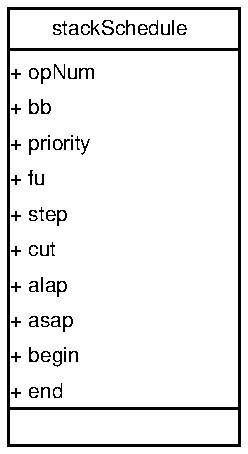
\includegraphics{figures/stackSchedule.pdf}
}{
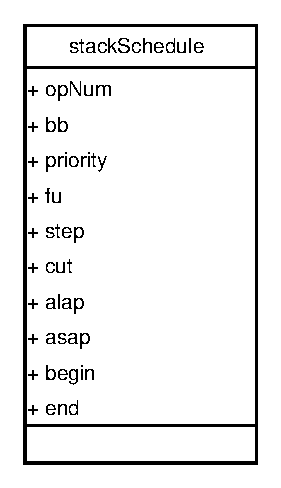
\includegraphics{figures/stackSchedule.eps}
}
\ccaption{Diagramma della classe stackSchedule}
\label{f:stackSchedule}
\end{figure}

\subsubsection{FDschedule}
Un oggetto di questa classe memorizza i dati di un possibile assegnamento non ancora effettuato. All'interno di esso sono memorizzati:
\begin{itemize}
\item i dati relativi all'operazione: identificatore, blocco basico di appartenenza, priorit�;
\item i dati relativi all'assegnamento: tipo di unit� funzionale, passo di controllo e se � bloccato o meno;
\item il valore della forza corrispondente;
\item la finestra temporale influenzata da questo assegnamento, cio� i passi di controllo in cui la percentuale di occupazione riferita a qualche tipo di unit� funzionale � stata modificata a seguito dell'assegnamento stesso; questi passi di controllo coincidono con quelli in cui la variazione della percentuale di occupazione relativa ad un tipo di unit� funzionale potrebbe provocare la variazione di forza relativa all'assegnamento contenuto nell'istanza; questi dati sono utilizzati dall'algoritmo per evitare di ricalcolare ad ogni iterazione tutte le forze e limitarsi al calcolo di quelle modificate dall'ultimo assegnamento o dall'ultima cancellazione di un assegnamento.
\end{itemize}

\begin{figure}[h!]
\centering
\ifthenelse{\boolean{pdf}}
{
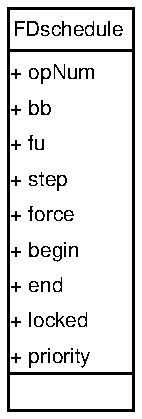
\includegraphics{figures/FDschedule.pdf}
}{
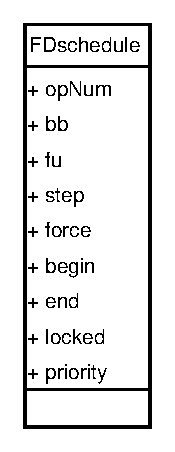
\includegraphics{figures/FDschedule.eps}
}
\ccaption{Diagramma della classe FDschedule}
\label{f:FDschedule}
\end{figure}

\subsubsection{infOp\_type}
Un oggetto di questa classe memorizza i dati relativi alla percentuale di occupazione di un certo tipo di unit� funzionale da parte di un'operazione in un passo di controllo. Da questi dati si ricavano le percentuali di occupazione complessive. La coppia <unit� funzionale-passo di controllo> non � indicata al suo interno perch� la classe \verb|force_directed| costruisce una lista di \verb|infOp_type| diversa per ciascuna coppia. All'interno di un'istanza di \verb|infOp_type| vengono memorizzati:
\begin{itemize}
\item i dati dell'operazione: identificatore, blocco basico di appartenenza e se � gia stata assegnata;
\item la percentuale di occupazione;
\item l'elenco dei blocchi basici in mutua esclusione con quello dell'operazione indicata nell'istanza stessa e ai quali appartiene almeno un'operazione schedulabile con probabilit� non nulla nello stesso passo di controllo e sullo stesso tipo di unit� funzionale del possibile assegnamento sottinteso dall'istanza stessa; queste liste sono utilizzate per limitare il numero di blocchi basici da collassare durante il calcolo delle percentuali di occupazione nel caso di presenza di costrutti condizionali (\ref{c:impl:force:prob});
\item nel caso di operazioni multiciclo se l'operazione pu� essere schedulata nel passo di controllo sottinteso o se l'occupazione dell'unit� funzionale si riferisce ad una operazione schedulabile nei passi di controllo precedenti la cui esecuzione potrebbe non essere ancora terminata nel passo di controllo sottinteso.
\end{itemize}

\begin{figure}[h!]
\centering
\ifthenelse{\boolean{pdf}}
{
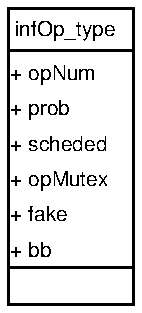
\includegraphics{figures/infOp_type.pdf}
}{
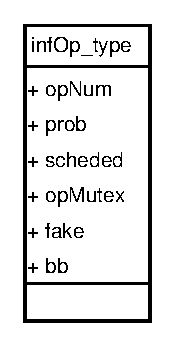
\includegraphics{figures/infOp_type.eps}
}
\ccaption{Diagramma della classe infOp\_type}
\label{f:infOp}
\end{figure}

\subsubsection{job}
Un oggetto di questa classe memorizza i dati relativi alla restrizione di un predecessore o di un successore a seguito di uno scheduling. Ogni volta che si calcola una forza viene creata una lista di questi oggetti per memorizzare la restrizione della finestra di mobilit� di ogni predecessore o successore; per ciascuna restrizione si dovr� calcolare il contributo alla \emph{predecessors' and successors' force} corrispondente. 

Dopo aver calcolato il contributo relativo alla restrizione della finestra di un predecessore (successore), si calcolano anche le eventuali riduzioni di mobilit� cui sono soggetti i suoi diretti predecessori (successori) e si aggiungono alla lista. Mantenendo gli oggetti ordinati in base all'ordinamento topografico delle operazioni nel SDG (questo se si riferiscono a restrizioni delle mobilit� dei successori; per i predecessori l'ordine � quello inverso) si garantisce che il contributo di forza relativo ad un predecessore o ad un successore verr� calcolato un'unica volta. Infatti se si fossero usate tecniche ricorsive per il calcolo delle forze poteva accadere per esempio che il contributo di un predecessore, se questo era legato tramite due diversi percorsi all'operazione di cui si sta calcolando la forza, venisse considerato due volte. Le informazioni memorizzate da un oggetto di questa classe sono:
\begin{itemize}
\item identificatore dell'operazione;
\item posizione dell'operazione nell'ordinamento topologico del SDG;
\item nuova finestra temporale dell'operazione a seguito dell'ipotesi di assegnamento;
\item mobilit� dell'operazione a seguito dell'ipotesi di assegnamento (esplicitata per permettere l'ordinamento fra due istanze relative alla stessa operazione).
\end{itemize}


\begin{figure}[h!]
\centering
\ifthenelse{\boolean{pdf}}
{
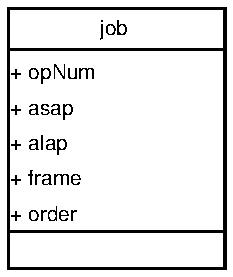
\includegraphics{figures/job.pdf}
}{
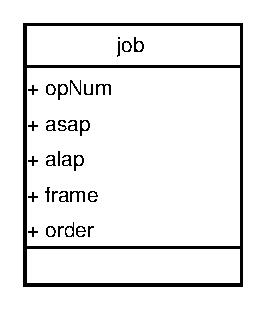
\includegraphics{figures/job.eps}
}
\ccaption{Diagramma della classe job}
\label{f:job}
\end{figure}

\subsubsection{force\_directed}
La classe \verb|force_directed| implementa il Force Directed scheduling; eredita come tutti gli algoritmi di scheduling implementati in PandA dalla classe \verb|scheduling|. Le strutture dati contenute in essa memorizzano:
\begin{itemize}
\item i dati del problema di scheduling:
\begin{itemize}
\item il grafo SDG;
\item le caratteristiche delle unit� funzionali e i vincoli sul loro numero;
\item l'ordinamento topologico, il tipo, l'ASAP e l'ALAP delle operazioni;
\item le caratteristiche dei diversi tipi di operazione;
\end{itemize}
\item la priorit� assegnata alle operazioni;
\item il grado attuale dell'albero di ricerca;
\item il criterio di scelta del prossimo assegnamento selezionato;
\item le operazioni gi� assegnate e il numero di operazioni ancora da assegnare;
\item il numero di soluzioni anche parziali che non soddisfano i vincoli incontrate durante la ricerca;
\item l'elenco delle mutue esclusioni fra blocchi basici e fra operazioni;
\item per ciascun tipo di unit� funzionale il numero utilizzato in ciascun passo di controllo e il binding delle operazioni sulle unit� funzionali;
\item le forze relative a tutti gli assegnamenti possibili;
\item le percentuali di occupazione, totali e relative alle singole operazioni, dei diversi tipi di unit� funzionale nei diversi passi di controllo.
\end{itemize}

La classe oltre al costruttore fornisce due metodi pubblici: il primo computa l'algoritmo, il secondo stampa informazioni riguardo ad esso. I metodi privati invece sono pi� numerosi; i servizi che essi offrono sono:
\begin{itemize}
\item inizializzazione delle strutture dati riguardanti i dati del problema di scheduling;
\item inizializzazione delle strutture dati riguardanti le unit� funzionali;
\item eliminazione di un'operazione dalle liste contenenti le percentuali di occupazione relative;
\item inserimento di un'operazione nelle liste contenenti le percentuali di occupazione relative;
\item calcolo delle mutue esclusioni fra operazioni schedulabili in un certo passo di controllo;
\item calcolo delle percentuali di occupazione totali;
\item restrizione della finestra temporale di un'operazione e conseguente ricalcolo delle percentuali di occupazione;
\item calcolo degli immediati predecessori di un'operazione;
\item calcolo degli immediati successori di un'operazione;
\item calcolo della forza di un assegnamento;
\item calcolo della \emph{self-force} di un assegnamento;
\item calcolo delle \emph{predecessors' and successors' force} di un assegnamento;
\item calcolo del prossimo assegnamento da effettuare;
\item calcolo del miglior tempo di esecuzione di un'operazione;
\item calcolo del binding di un'operazione su un'unit� funzionale;
\item cancellazione di un binding gi� effettuato.
\end{itemize}


\newpage
\begin{figure}[h!]
\centering
\ifthenelse{\boolean{pdf}}
{
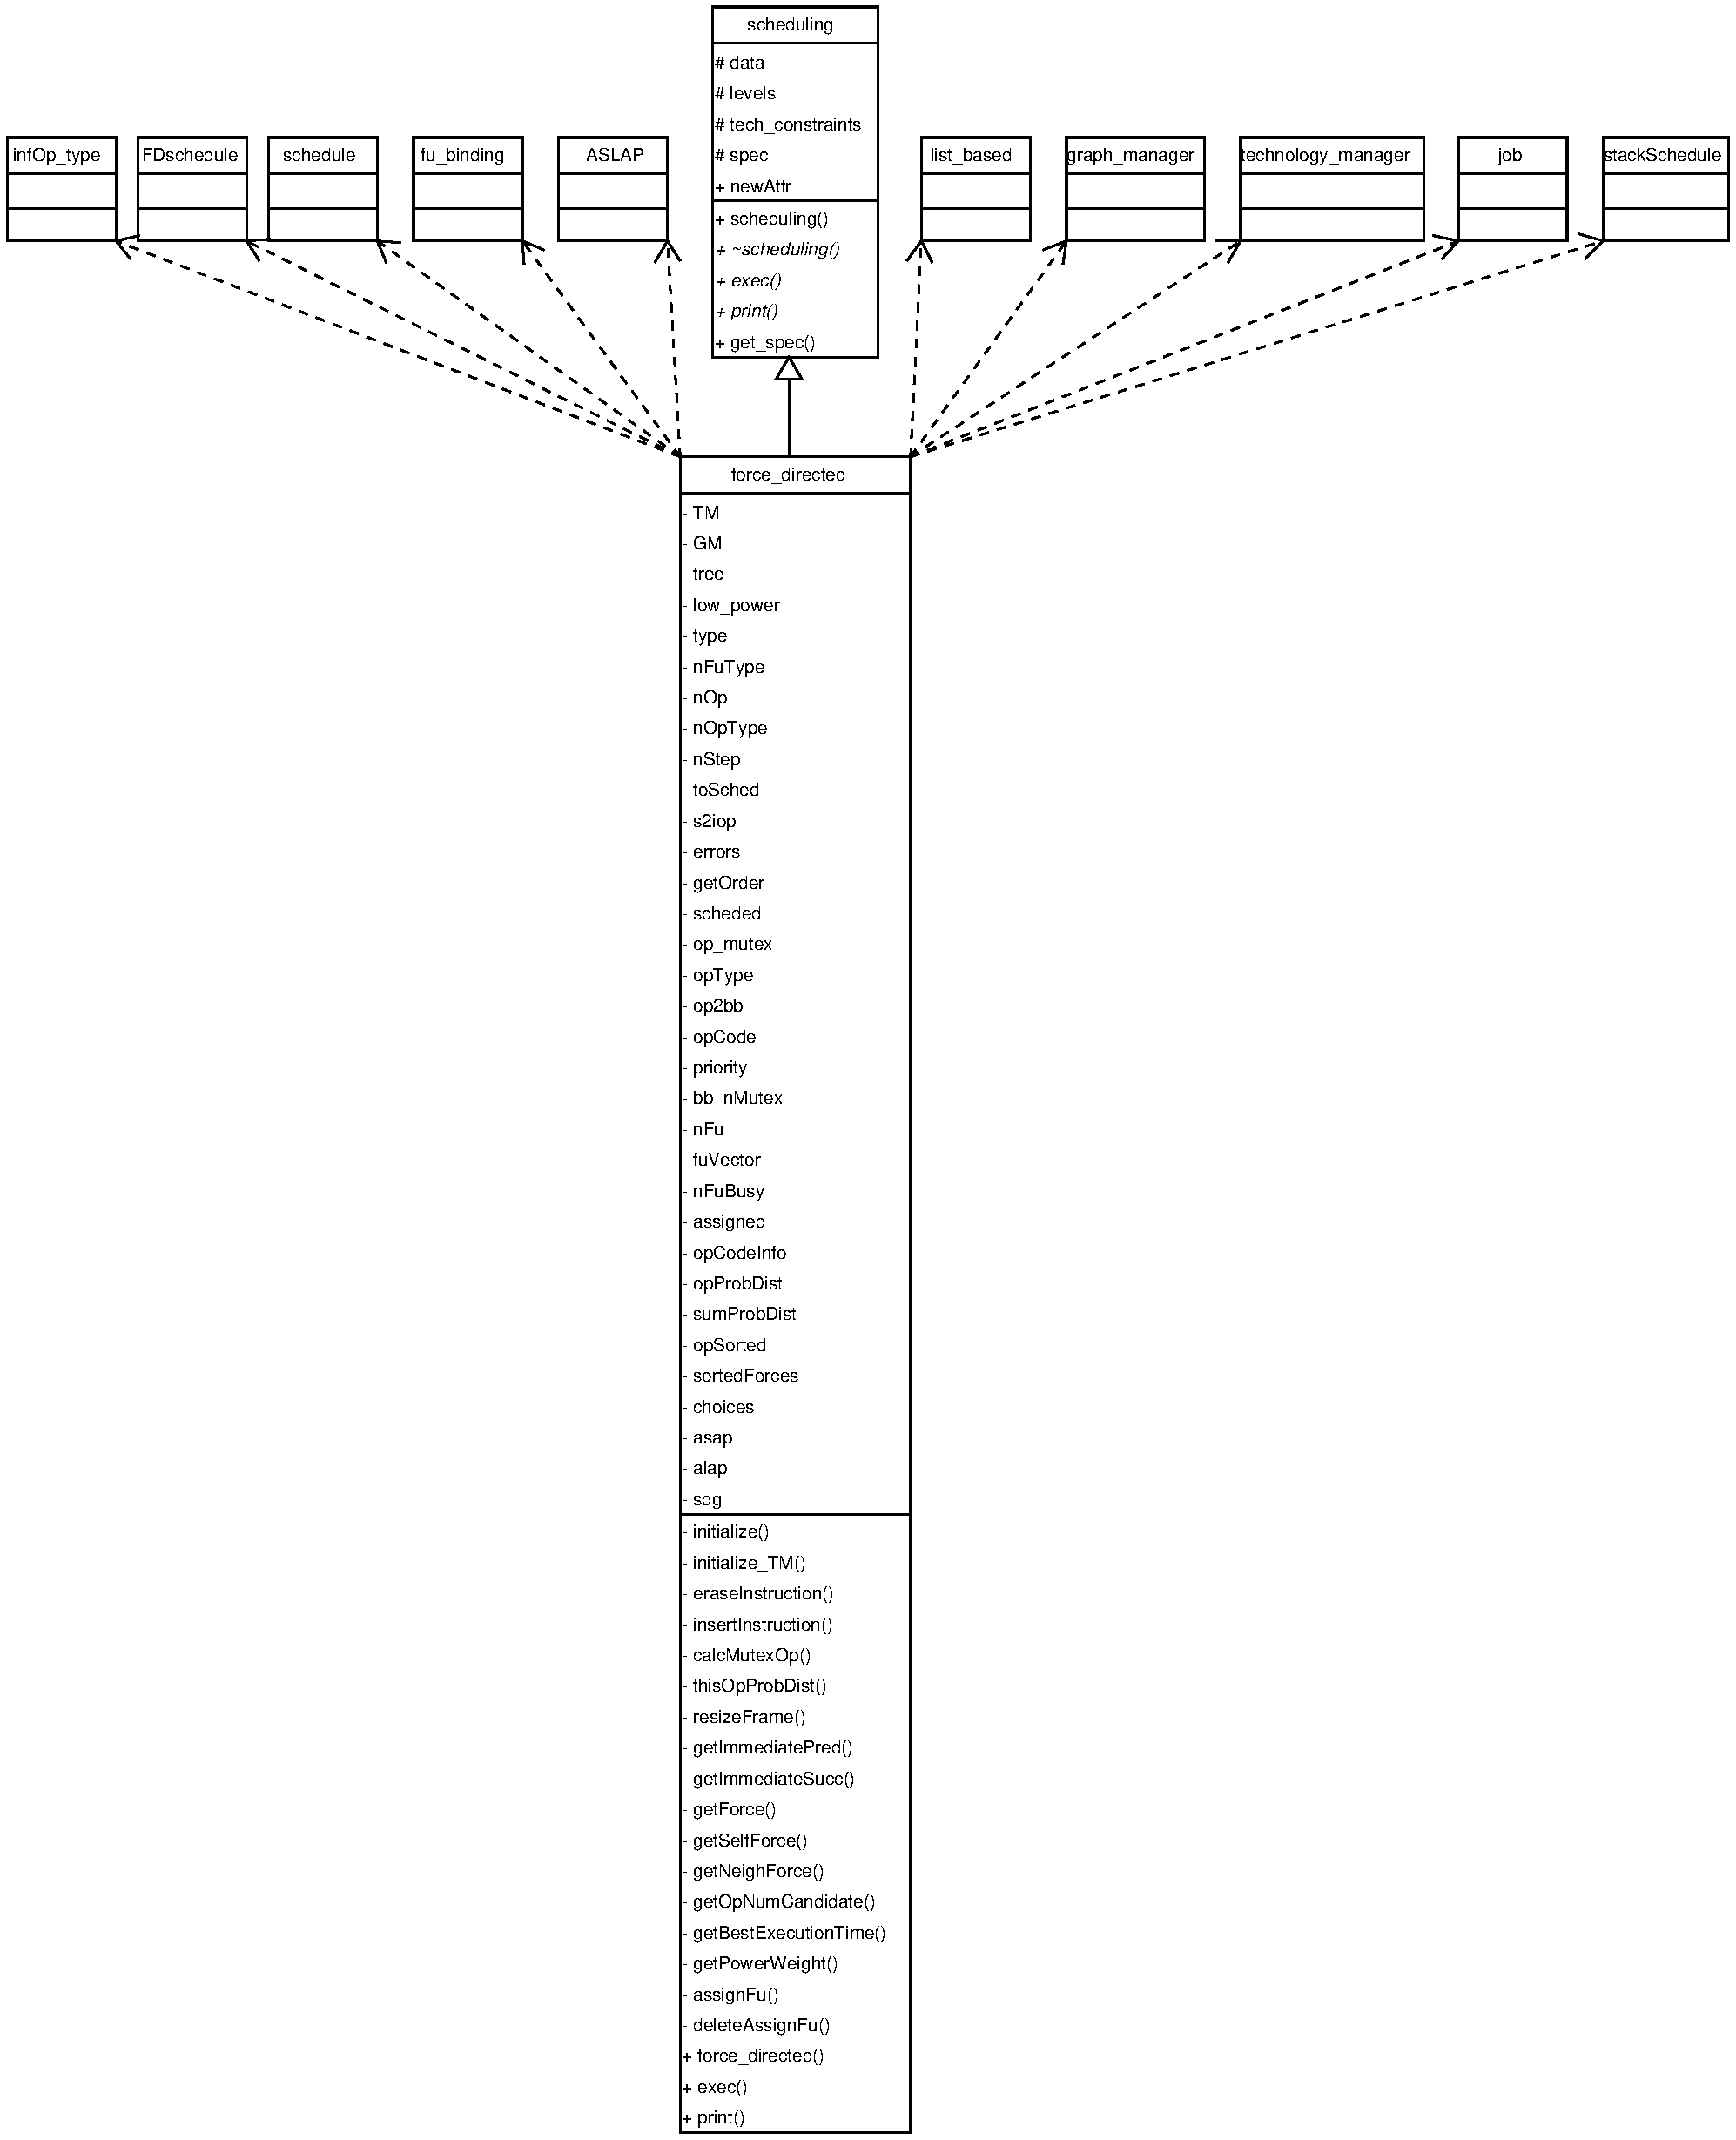
\includegraphics[scale = 0.4]{figures/force_directed.pdf}
}{
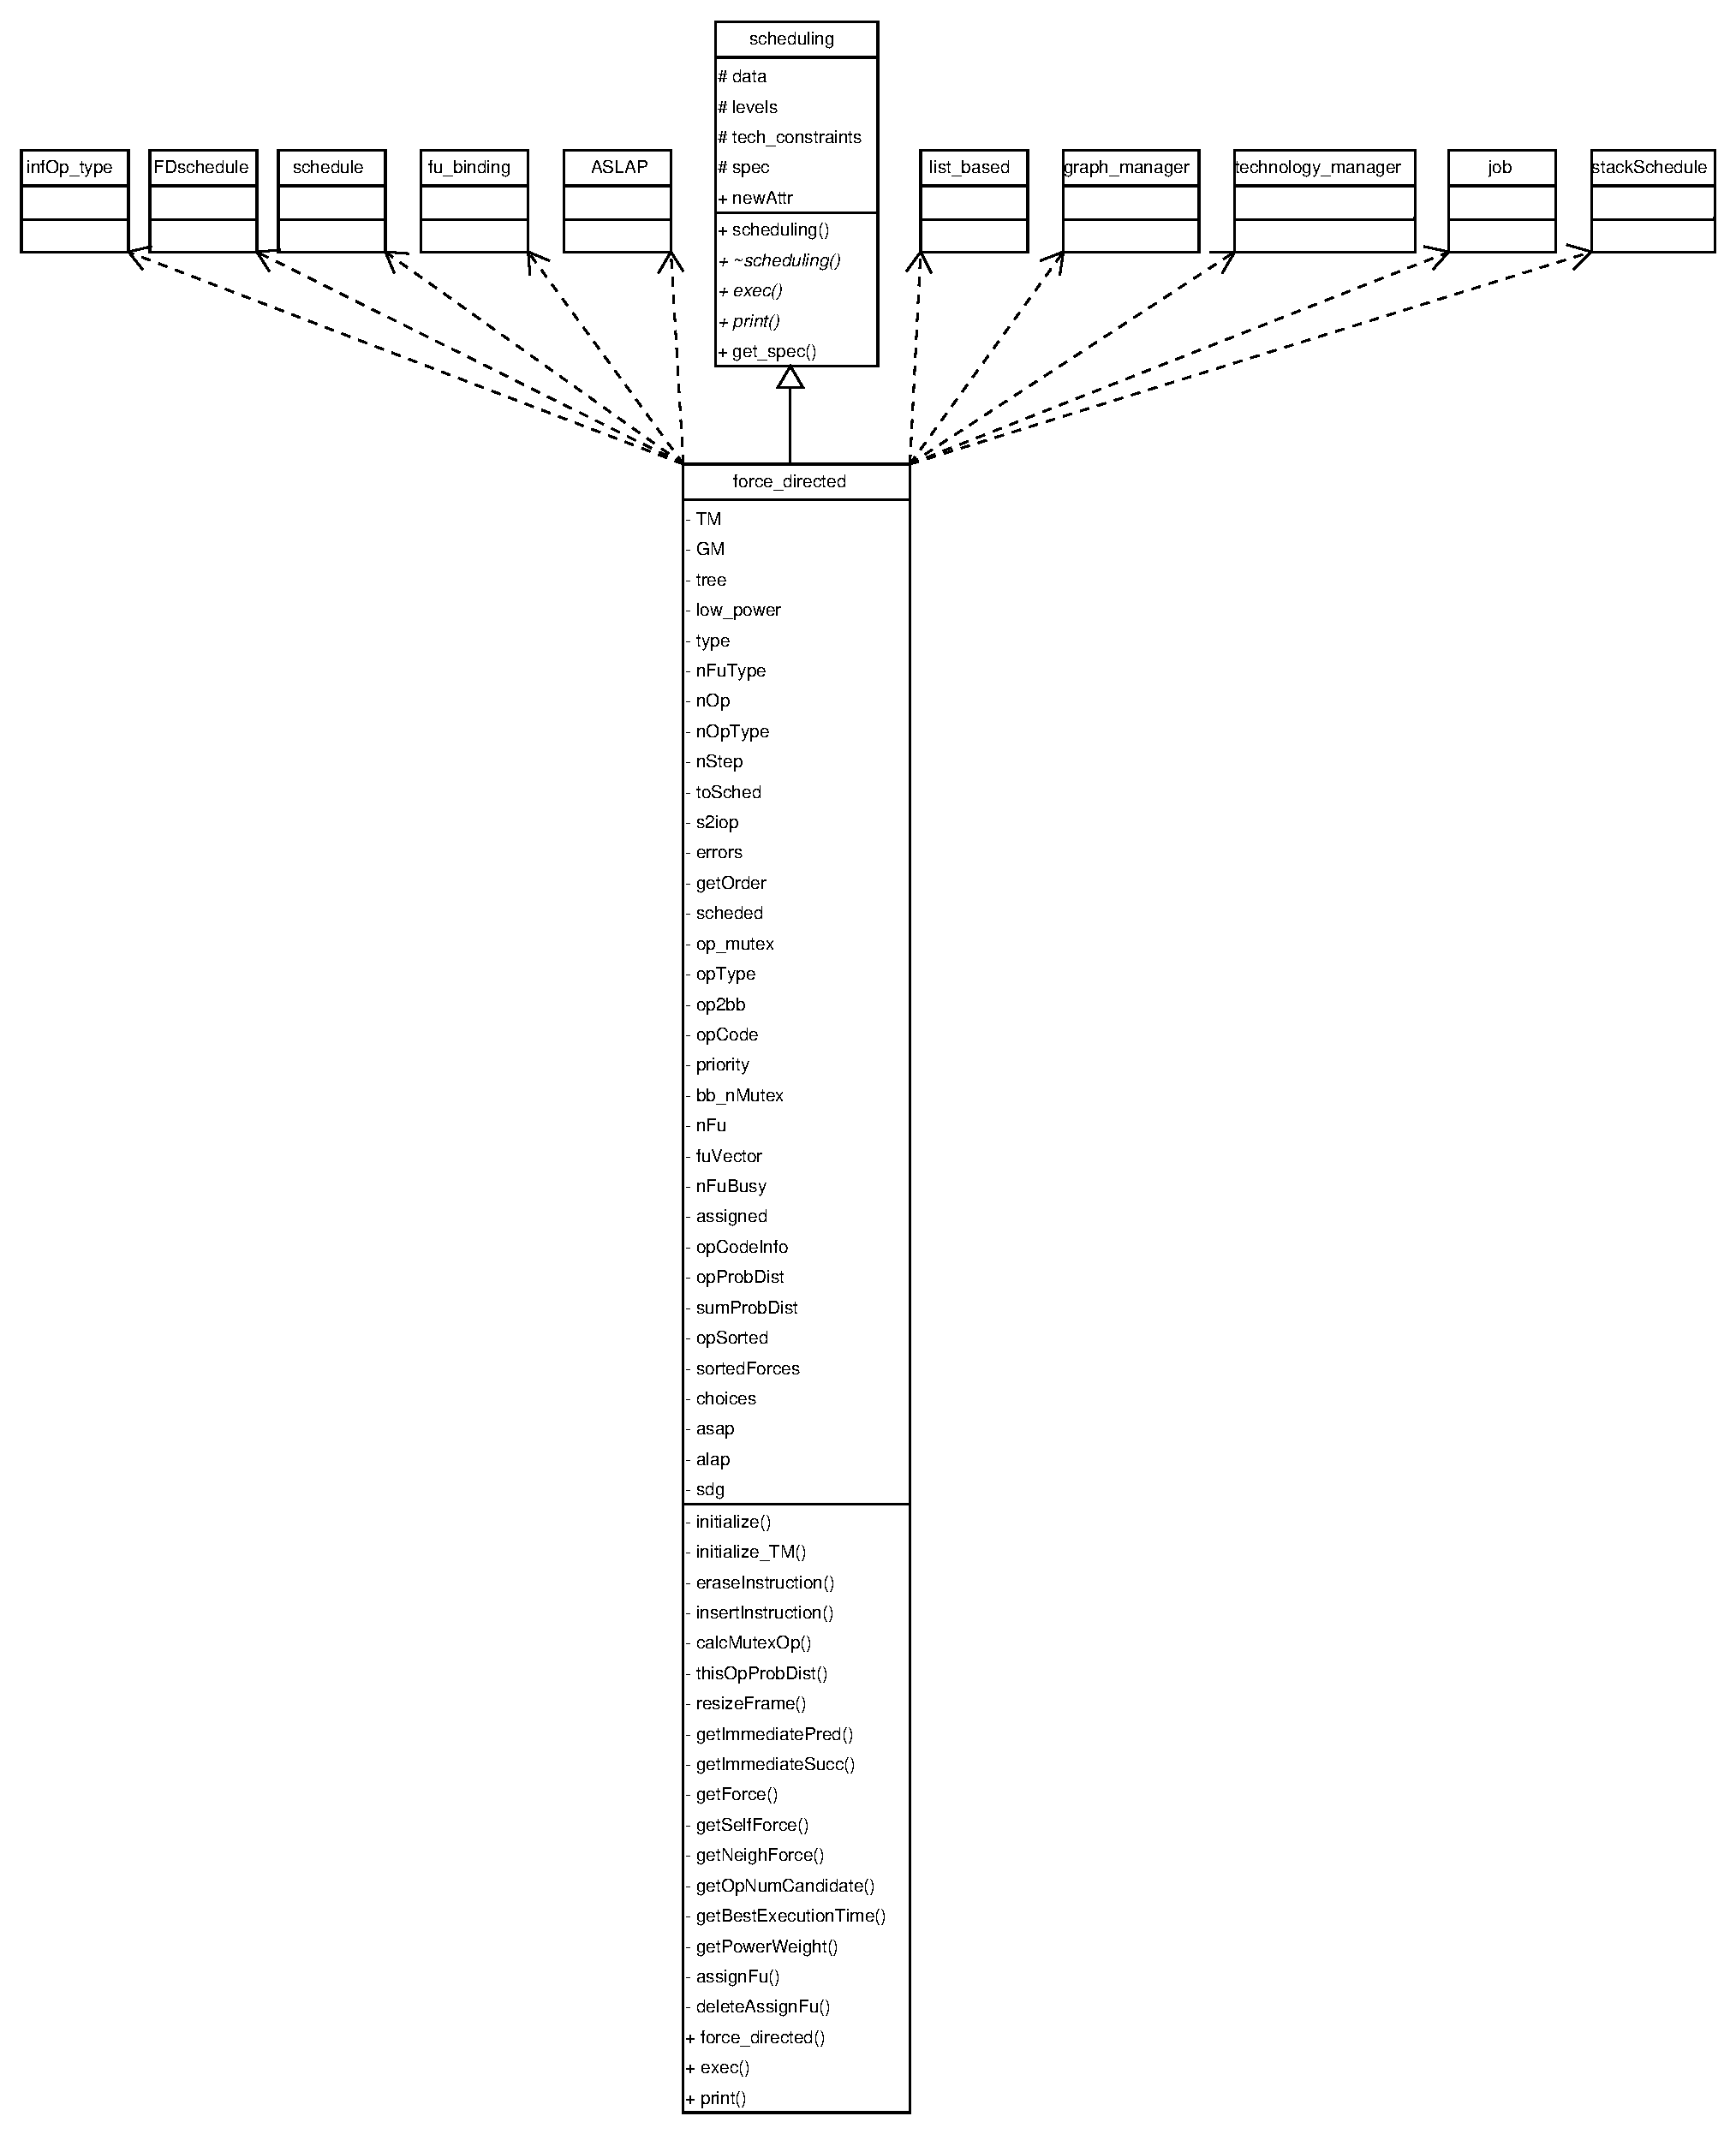
\includegraphics[scale = 0.4]{figures/force_directed.eps}
}
\ccaption{Diagramma della classe force\_directed}
\label{f:force}
\end{figure}

\newpage
\subsection{Calcolo delle somme di probabilit�}
\label{c:impl:force:prob}
Viene ora fornita la soluzione adottata nell'implementazione per risolvere il problema di calcolare le somme di probabilit� (e quello equivalente di calcolare le percentuali di occupazione) indicate in \ref{c:ori:core:prob}. Questo sia perch� da un punto di vista implementativo questa funzione risulta la pi� critica, sia perch� in letteratura non si trovano descrizioni di possibili metodi per risolvere questo particolare problema ed esso non � di facile soluzione se non con metodi esaustivi e quindi di complessit� esponenziale. 

La funzione lavora su liste di operazioni che possono essere eseguite da un tipo di unit� funzionale in un determinato passo di controllo. Tali operazioni sono ordinate secondo due chiavi:
\begin{enumerate}
\item il numero di blocchi basici che sono in mutua esclusione con quello dell'operazione e a cui appartiene almeno un'altra operazione della lista;
\item l'ordinamento lessicografico (secondo la rappresentazione interna) del blocco basico cui appartengono.
\end{enumerate}
La prima chiave, per la quale si usa l'ordinamento decrescente (l'ordinamento utilizzato per la seconda chiave � ininfluente cos� come l'ordinamento fra operazioni che abbiano le stesse chiavi), che � facilmente calcolabile, comporta che i blocchi basici che costituiscono i diversi rami dei costrutti condizionali annidati pi� internamente si trovino nelle prime posizioni della lista, mentre i blocchi basici relativi a segmenti non condizionati del problema si trovano nella sua parte terminale.

Per ogni blocco basico, una cui operazione � presente nella lista, si crea una struttura dati che contiene le informazioni relative al blocco basico stesso, le due chiavi utilizzate per l'ordinamento delle operazioni, una lista di quali siano i blocchi basici con cui esso � in mutua esclusione e un valore detto probabilit� pari alla somma delle probabilit� delle operazioni che si trovano nella lista e che appartengono a quel blocco basico. I blocchi basici che hanno la prima chiave pari a zero vengono trascurati e la probabilit� delle operazioni ad essi appartenenti viene sommata direttamente alla soluzione finale che inizialmente � posta pari a zero. Gli altri blocchi basici vengono ordinati in una nuova lista con lo stesso tipo di ordinamento illustrato per le operazioni.

A questo punto scorrendo la lista si individua la coppia di blocchi basici appartenenti ai rami di uno dei costrutti condizionali pi� annidati e si collassano: le informazioni del nuovo blocco basico coincideranno con quelle di uno qualsiasi dei due ad eccezione della probabilit� che sar� pari al valore maggiore fra le due. Il blocco basico cos� creato potrebbe trovarsi concatenato con uno o pi� blocchi basici (concatenazione in questo senso: due o pi� blocchi basici sono concatenati se sono legati da archi di controllo e nessun altro blocco basico ad eccezione dei predecessori del primo e dei successori dell'ultimo � legato con un arco di controllo ad uno di essi). I blocchi concatenati si fondono mantenendo le informazioni di uno qualsiasi di essi ad eccezione della probabilit� che viene posta pari alla sommatoria di quelle dei blocchi originari. In questo modo � come se nel grafo dei blocchi basici fosse stata eliminata la biforcazione relativa al costrutto condizionale pi� annidato. Ad ogni iterazione si mantiene ordinata la lista dei blocchi basici che vede ridursi il numero dei suoi elementi. A questo punto basta applicare ripetutamente quanto descritto fino ad eliminare la biforcazione nel grafo relativa all'ultimo costrutto condizionale superstite. La probabilit� del blocco superstite verr� sommata a quella della soluzione ottenuta fino a quel momento ottenendo cos� il valore definitivo.

La complessit� di questo metodo � pari a $O(B^4)$ dove $B$ � il numero dei blocchi basici presenti nel grafo omonimo.

\subsection{Calcolo della mutua esclusione fra le operazioni}
Un altro aspetto critico nell'implementazione dell'algoritmo � la parte che riguarda il calcolo delle mutue esclusioni fra operazioni. La soluzione proposta lavora a livello di blocchi basici (se due operazioni appartengono a due blocchi basici in mutua esclusione allora saranno esse stesse in mutua esclusione) e si basa sull'Albero dei Dominatori.

Inizialmente si compie una visita inversa breadth-first dell'Albero dei Dominatori durante la quale si memorizzano i discendenti di ciascun nodo. A questo punto si esegue nuovamente una visita breadth-first (questa volta non inversa) dell'Albero dei Dominatori. Gli assegnamenti da compiere durante la seconda visita si differenziano a seconda del tipo di blocco basico:

\begin{itemize}
\item Nodo Radice:

nessun assegnamento

\item Nodo di un blocco basico corrispondente ad un ramo then:

la lista dei blocchi basici con cui esso � in esclusione � posta uguale all'unione di:
\begin{itemize}
\item il blocco basico che corrisponde ad un ramo else e il cui nodo � fratello di quello del nodo in oggetto (se presente);
\item i discendenti del blocco basico indicato al punto precedente (se presente) che sono gi� stati calcolati durante la prima visita;
\item i blocchi basici in mutua esclusione con il blocco basico rappresentato dal genitore del nodo in oggetto; sono gi� stati calcolati perch� la seconda visita � discendente.
\end{itemize}

\item Nodo di un blocco basico corrispondente ad un ramo else:

la lista dei blocchi basici con cui esso � in esclusione � posta uguale all'unione di:
\begin{itemize}
\item il blocco basico che corrisponde ad un ramo then e il cui nodo � fratello di quello del nodo in oggetto;
\item i discendenti del blocco basico indicato al punto precedente che sono gi� stati calcolati durante la prima visita;
\item i blocchi basici in mutua esclusione con il blocco basico rappresentato dal genitore del nodo in oggetto; sono gi� stati calcolati perch� la seconda visita � discendente.
\end{itemize}

\item Nodo di un blocco basico di tipo endif:

la lista dei blocchi basici con cui esso � in esclusione � posta uguale alla lista delle mutue esclusioni del padre gi� calcolata.
\end{itemize}
\chapter{Risultati Sperimentali}
\label{c:res}
\thispagestyle{empty}

\vspace{0.5cm}

In questo capitolo vengono presentati i risultati sperimentali ottenuti utilizzando l'algoritmo del Force Directed scheduling modificato proposto nel capitolo \ref{c:my} confrontati con quelli della versione originale dell'algoritmo e con quelli forniti dal List-Based. I test sono stati fatti utilizzando l'implementazione realizzata all'interno di PandA. I benchmark utilizzati sono quelli forniti con PandA stesso, in particolare quelli forniti sotto forma di moduli scritti in codice c. La macchina utilizzata per i test � un portatile basato su architettura Intel Sonoma con processore a 1,83 Ghz e 1 GB di memoria RAM PC4300.

In particolare i risultati analizzati sono quelli riferiti a:
\begin{itemize}
\item tempo di esecuzione;
\item numero totale di unit� funzionali allocate; il numero fornito � quello totale senza discriminazione fra i diversi tipi di unit� funzionale perch� non sono stati inseriti nei dati relativi all'architettura i costi delle diverse unit� funzionali, quindi per l'algoritmo minimizzare l'utilizzo di un particolare tipo di un'unit� funzionale piuttosto che un altro � irrilevante. Unica eccezione sono i casi caratterizzati dalla presenza di vincoli in cui l'algoritmo distingue fra unit� vincolate e unit� non vincolate (\ref{c:res:vincoli}).
\end{itemize}
In alcuni casi al posto del tempo di esecuzione � riportato il termine "MAX". Questo sta a significare che quella computazione dell'algoritmo ha richiesto pi� di un migliaio di secondi. In tal caso si � ritenuto che il tempo di esecuzione fosse comunque troppo elevato e quindi non significativo. Un tempo di esecuzione cos� elevato pu� manifestarsi solo nel caso di un elevato numero di backtracking e quindi in caso di presenza di vincoli sulle risorse. In particolare si � riscontrato questo problema nell'esecuzione della versione pseudo-originale del Force Directed scheduling (per versione pseudo-originale si intende la versione originale cui sono state fatte leggere modifiche per permettere di aggiungere il backtracking e consentire cos� di eliminare le soluzioni non accettabili).

Per il numero relativamente elevato delle modifiche introdotte sono state effettuate sessioni di test diverse per mostrare gli incrementi relativi a singole variazioni o a gruppi di esse.

Nelle tabelle con \emph{nFU} si indica il numero totale di unit� funzionali allocate dall'algoritmo, con \emph{tempo} il tempo necessario per la computazione dello scheduling in secondi.

\newpage

\section{Dimensioni dei benchmark}
Si riportano numero di operazioni e numero di salti condizionati presenti nei benchmark utilizzati per testare le diverse versioni dell'algoritmo:

\begin{table}[!h]
\begin{center}
\begin{tabular}{|l|c|c|}
\hline
Benchmark & nOp & n� salti\\
\hline
Adpcm\_decode & 68 & 11 \\
Adpcm\_encode & 83 & 14 \\
Arf & 34 & 0 \\
Bandpass & 52 & 0 \\
Chemical & 38 & 0 \\
ComputeForwVector & 77 & 14 \\
Dct & 58 & 0 \\
Dct\_wang & 57 & 0 \\
Diffeq & 27 & 1 \\
Ewf & 39 & 0 \\
Ewf\_v2 & 55 & 0 \\
Kim & 34 & 2 \\
Maha & 30 & 5 \\
\hline
\end{tabular}
\end{center}
\ccaption{Numero di operazioni e di salti condizionati di ogni benchmark}
\label{tab4}
\end{table}

\section{Variazioni nel calcolo della forza}
Vengono qui proposti i risultati sperimentali che mostrano i guadagni nella qualit� dei risultati ottenuti tramite la modifica della formula per il calcolo della forza introducendo la variazione della somma di probabilit� al posto della variazione della probabilit� della singola operazione (\ref{c:my:var:force}) e limitando il contributo dovuto a \emph{predecessors' and successors' forces} negative (\ref{c:my:var:corr}).

In particolare per i test in tabella \ref{tabnew2}, in cui non sono presenti costrutti condizionali, l'unica variazione effettiva � quella prodotta dalla variazione nel calcolo delle \emph{predecessors' and successors' forces}.

\begin{table}[!h]
\begin{center}
\begin{tabular}{|l|c c|c c|}
\hline
Benchmark & \multicolumn{2}{c|}{FD Orig.} & \multicolumn{2}{c|}{FD Modif.} \\
& nFU & tempo & nFU & tempo \\
\hline
Arf & 14 & 0.23 & 8 & 0.25 \\
Bandpass & 20 & 0.55 & 11 & 0.57 \\
Chemical & 25 & 0.45 & 15 & 0.69 \\
Dct & 35 & 0.80 & 20 & 1.03 \\
Dct\_wang & 29 & 0.65 & 20 & 0.85 \\
\hline
\end{tabular}
\end{center}
\ccaption{Tabella comparativa calcolo Forza originale - calcolo Forza modificato nei test senza costrutti condizionali}
\label{tabnew2}
\end{table}

I test di tabella \ref{tabnew} presentando anche costrutti condizionali mostrano invece anche i miglioramenti dovuti all'introduzione della variazione della somma di probabilit�.

\begin{table}[!h]
\begin{center}
\begin{tabular}{|l|c c|c c|}
\hline
Benchmark & \multicolumn{2}{c|}{FD Orig.} & \multicolumn{2}{c|}{FD Modif.} \\
& nFU & tempo & nFU & tempo \\
\hline
Adpcm\_decode & 27 & 2.89 & 18 & 10.69 \\
Adpcm\_encode & 27 & 5.84 & 19 & 43.68 \\
Diffeq & 14 & 0.09 & 8 & 0.29 \\
Kim & 9 & 0.46 & 6 & 0.73 \\
Maha & 10 & 0.39 & 5 & 0.43 \\
\hline
\end{tabular}
\end{center}
\ccaption{Tabella comparativa calcolo Forza originale - calcolo Forza modificato nei test con costrutti condizionali}
\label{tabnew}
\end{table}

Apparentemente il guadagno in termini di unit� funzionali risparmiate � notevole, tale da giustificare largamente l'aumento del tempo di esecuzione. Tale aumento � dovuto in primo luogo alla maggiore complessit� introdotta nel calcolo della forza dovuta al calcolo della differenza della somma di probabilit� e in secondo luogo al fatto che nella versione originale dell'algoritmo la mobilit� delle operazioni si riduce molto pi� velocemente, quindi diminuisce pi� velocemente il numero di forze da calcolare. Il guadagno � in realt� meno sostanziale di quanto appaia perch� la diminuzione riguarda anche, ma non solo, l'utilizzo di pseudo-unit� funzionali che vengono introdotte per eseguire pseudo-operazioni aggiunte dal gcc nella sua rappresentazione interna. Di fatto in alcuni casi l'area occupata da queste pseudo-unit� � nulla. Il guadagno in termini di costo d'area nei test proposti � quindi pi� limitato di quanto appaia inizialmente, ma comunque significativo.

\section{Introduzione della priorit� delle operazioni}
Vengono qui proposti i risultati sperimentali che mostrano i guadagni dovuti all'introduzione della priorit� delle operazioni mostrata in \ref{c:my:var:priority}. Ovviamente i test comparativi sono stati effettuati solo su benchmark che presentano costrutti condizionali in quanto in assenza di questi i risultati restano identici (a meno di una leggera maggiorazione nei tempi di computazione dovuta alla gestione delle strutture dati necessarie a memorizzare la priorit� delle operazioni). In entrambe le versioni sono state applicate le modifiche suggerite in \ref{c:my:var:force} e \ref{c:my:var:corr}
(correzione nel calcolo della forza).

\begin{table}[!h]
\begin{center}
\begin{tabular}{|l|c c|c c|}
\hline
Benchmark & \multicolumn{2}{c|}{FD Orig.} & \multicolumn{2}{c|}{FD Modif.} \\
& nFU & tempo & nFU & tempo \\
\hline
Adpcm\_decode & 18 & 11.77 & 18 & 3.54 \\
Adpcm\_encode & 19 & 43.30 & 19 & 7.92 \\
Diffeq & 8 & 0.28 & 8 & 0.25 \\
Kim & 6 & 0.68 & 6 & 0.58 \\
Maha & 5 & 0.41 & 5 & 0.25 \\
\hline
\end{tabular}
\end{center}
\ccaption{Tabella comparativa \mbox{Force Directed} senza priorit� - \mbox{Force Directed} con Priorit�}
\label{tab3}
\end{table}
Come � facile osservare il guadagno in termini di velocit� nella computazione senza perdite di qualit� di risultati � significativo soprattutto per quei problemi con numero elevato di operazioni e numero medio di operazioni per blocco basico basso.

\section{Cambio del criterio di scelta del prossimo assegnamento}
I risultati dei test effettuati hanno evidenziato che il miglior criterio di scelta del prossimo assegnamento fra quelli proposti in \ref{c:my:vincoli:next} � l'ultimo di quelli elencati (questo in particolare riferendosi ai test mostrati in \ref{c:test1}; per quanto riguarda i test proposti in \ref{c:test2} i diversi criteri di scelta del prossimo assegnamento danno risultati identici in quanto non esistendo vincoli non esistono neppure forze bloccate), cio� considerare pari a zero al fine del calcolo della forza media le forze bloccate. Si mostrano i risultati relativi a due classi diverse di problemi:
\subsection{Test senza vincoli sulle risorse}
\label{c:test2}
\begin{table}[!h]
\begin{center}
\begin{tabular}{|l|c c|c c|}
\hline
Benchmark & \multicolumn{2}{c|}{FD Orig.} & \multicolumn{2}{c|}{FD Modif.} \\
& nFU & tempo & nFU & tempo \\
\hline
Adpcm\_decode & 18 & 3.49 & 18 & 4.33 \\
Adpcm\_encode & 19 & 7.93 & 20 & 8.04 \\
Arf & 8 & 0.21 & 8 & 0.21 \\
Bandpass & 11 & 0.60 & 11 & 0.57 \\
Chemical & 15 & 0.64 & 15 & 0.68 \\
Dct & 20 & 0.94 & 20 & 0.82 \\
Dct\_wang & 20 & 0.81 & 20 & 0.78 \\
Diffeq & 8 & 0.24 & 9 & 0.22 \\
Kim & 6 & 0.56 & 5 & 0.58 \\
Maha & 5 & 0.25 & 5 & 0.25 \\
\hline
\end{tabular}
\end{center}
\caption{Tabella comparativa criterio di scelta del prossimo assegnamento - casi senza vincoli}
\label{tab6}
\end{table}

I risultati riportati in tabella \ref{tab6} mostrano che in realt� il cambiare il criterio di scelta del prossimo assegnamento non comporta grandi differenze nei risultati sia dal punto di vista del numero di unit� funzionali allocate, sia dal punto di vista del tempo di computazione. Tuttavia la versione finale dell'algoritmo proposta offre un criterio di assegnamento diverso da quello originario, nonostante per questa classe di problemi non comporti un effettivo guadagno, in virt� dei risultati esposti nella successiva sottosezione.

\subsection{Test con vincoli sulle risorse}
\label{c:test1}
Vengono anticipati i risultati di alcuni test in caso di presenza di vincoli sulle risorse per giustificare il cambio nel criterio di scelta del prossimo assegnamento. I risultati riportati dimostrano il vantaggio in termini di tempo di esecuzione prodotto dal cambiamento di criterio. I vincoli imposti consistono nel fissare il numero di unit� funzionali a :
\begin{itemize}
\item[] 1 sommatore
\item[] 1 sottrattore
\item[] 1 moltiplicatore
\item[] 1 comparatore
\item[] 1 shifter
\item[] 2 unit� per accesso ad array 
\end{itemize}
I tipi di unit� non elencati sono considerati allocabili in numero infinito.

\begin{table}[!h]
\begin{center}
\begin{tabular}{|l|c c|c c|}
\hline
Benchmark & \multicolumn{2}{c|}{FD Orig.} & \multicolumn{2}{c|}{FD Modif.} \\
& nFU & tempo & nFU & tempo \\
\hline
Arf & 3 & 17.95 & 3 & 8.86 \\
Bandpass & 7 & 114.27 & 7 & 6.06 \\
Chemical & 5 & 35.41 & 6 & 21.86 \\
Dct & 6 & 90.03 & 5 & 103.58 \\
Dct\_wang &   & MAX & 9 & 192.97 \\
Ewf           &   &  MAX &  4 & 32.54 \\
\hline
\end{tabular}
\end{center}
\ccaption{Tabella comparativa criterio di scelta del prossimo assegnamento - casi con vincoli}
\label{tab7}
\end{table}
Da notare come la versione con criterio di scelta modificato trovi una soluzione in tempi ragionevoli anche nei casi in cui la versione che utilizza il criterio originale non riesca a trovarne una entro il tempo di 1000 secondi e che in generale utilizzi comunque meno tempo per la computazione. Il peggioramento nel numero di unit� di esecuzione allocate che si � verificato in un caso di test � relativo ad un'unit� in grado di eseguire le pseudo-operazioni e pertanto ha poca importanza per il costo in termini di area.

\section{Scheduling con vincoli sulle risorse}
Vengono ora proposti i risultati nel caso di vincoli con le risorse. Si confrontano tempo di esecuzione e numero di unit� allocate di due versioni diverse dell'algoritmo. I vincoli sono quelli riportati in \ref{c:test1}:
\begin{itemize}
\item 1� versione: Force Directed modificato con l'introduzione delle modifiche proposte in \ref{c:my:var:force}, \ref{c:my:var:corr} e \ref{c:my:vincoli:back} (correzione nel calcolo delle forze e introduzione del backtracking);
\item 2� versione: Force Directed modificato con tutte le variazioni proposte in questo lavoro.
\end{itemize}

\begin{table}[!h]
\begin{center}
\begin{tabular}{|l|c c|c c|}
\hline
Benchmark & \multicolumn{2}{c|}{FD 1� Vers.} & \multicolumn{2}{c|}{FD 2� Vers.} \\
& nFU & tempo & nFU & tempo \\
\hline
Adpcm\_decode & 15 & 19.06 & 14 &  7.36 \\
Adpcm\_encode & 12 & 93.98 & 14 & 30.82 \\
Arf           &  4 & 17.95 &  5 &  8.86 \\
Bandpass      &  7 &114.27 &  8 &  6.06 \\
Chemical      &  6 & 35.41 &  7 & 21.86 \\
ComputeForwVector & & MAX  & 11 & 15.73 \\
Dct           &  5 &103.58 &  6 & 90.03 \\
Dct\_wang     &    &   MAX &  9 &192.97 \\
Diffeq        &  7 &  1.06 &  8 &  0.94 \\
Ewf           &    &   MAX &  4 & 32.54 \\
Kim           &  5 &  1.28 &  5 &  0.55 \\
Maha          &  5 &  0.18 &  5 &  0.13 \\
\hline
\end{tabular}
\end{center}
\ccaption{Tabella comparativa nel caso di scheduling con vincoli sulle risorse}
\label{tab8}
\end{table}

I dati dicono che la seconda versione dell'algoritmo fornisce risultati mediamente leggermente peggiori nei casi in cui la prima versione produca la soluzione in tempo ragionevole. Tuttavia la seconda versione a differenza della prima ha prodotto una soluzione accettabile in tempo minore ai 1000 secondi in ogni test e comunque sempre in un tempo decisamente minore rispetto alla prima.

\section{Confronto con i risultati del List Based in caso di vincoli sulle risorse}
\label{c:res:vincoli}
In un buon numero di test il Force Directed scheduling ottiene gli stessi risultati in numero di unit� funzionali allocate del List Based con un tempo di computazione sensibilmente maggiore. Questo poich� in realt� le unit� funzionali pi� significative nei benchmark considerati erano gi� state vincolate e questo limita di molto le dimensioni dello spazio progettuale. Esistono tuttavia dei test in cui il Force Directed ha ottenuto una soluzione con un minor numero di unit� funzionali allocate.

I vincoli imposti per tali test sono:

\begin{itemize}
\item[] 2 sommatore
\item[] 2 sottrattore
\item[] 1 moltiplicatore
\item[] 2 comparatori
\item[] 1 shifter
\item[] 2 unit� per accesso ad array.
\end{itemize}

\subsection{Diminuzione delle unit� funzionali soggette a vincoli}
In questa sezione sono riportati due benchmark per i quali il Force Directed scheduling ha ottenuto per alcuni tipi di risorsa l'allocazione di un numero di unit� inferiore a quello imposto dai vincoli.
\subsubsection{Benchmark Kim}

\begin{table}[!h]
\begin{center}
\begin{tabular}{|l|c|c|c|}
\hline
Unit� Funzionale & Vincolo & LB & FD \\
\hline
indirect\_ref & inf & 1 & 2 \\
MINUS & 2 & 2 & 1 \\
PLUS & 2 & 2 & 2 \\
READ\_COND & inf & 1 & 1 \\
\hline
\multicolumn{2}{|l|}{Tempo computazione} & 0.11 & 0.18 \\
\hline
\end{tabular}
\end{center}
\ccaption{Unit� allocate per il benchmark Kim}
\label{tab9}
\end{table}
Il risultato � da considerarsi positivo in quanto essendo indirect\_ref una pseudo-operazione, l'area occupata da un'unit� funzionale che possa eseguirla � sensibilmente inferiore a quella occupata da un sottrattore.

\newpage
\subsubsection{Benchmark Maha}

\begin{table}[!h]
\begin{center}
\begin{tabular}{|l|c|c|c|}
\hline
Unit� Funzionale & Vincolo & LB & FD \\
\hline
CMP & 2 & 2 & 1 \\
indirect\_ref & inf & 1 & 1 \\
MINUS & 2 & 2 & 1 \\
PLUS & 2 & 1 & 1 \\
READ\_COND & inf & 2 & 1 \\
\hline
\multicolumn{2}{|l|}{Tempo computazione} & 0.14 & 0.12 \\
\hline
\end{tabular}
\end{center}
\ccaption{Unit� allocate per il benchmark Maha}
\label{tab10}
\end{table}

\subsection{Diminuzione delle unit� funzionali non soggette a vincoli}
In questa sezione sono riportati alcuni fra i benchmark per i quali il Force Directed scheduling ha ottenuto per alcuni tipi di risorse non vincolate l'allocazione di un numero di unit� inferiore a quello determinato dal List-Based.

\subsubsection{Benchmark Bandpass}

\begin{table}[!h]
\begin{center}
\begin{tabular}{|l|c|c|c|}
\hline
Unit� Funzionale & Vincolo & LB & FD \\
\hline
indirect\_ref & inf & 13 & 6 \\
MINUS         &   2 &  2 & 2 \\
MUL           &   1 &  1 & 1 \\
PLUS          &   2 &  1 & 2 \\
\hline
\multicolumn{2}{|l|}{Tempo computazione} & 0.22 & 75.77 \\
\hline
\end{tabular}
\end{center}
\ccaption{Unit� allocate per il benchmark Bandpass}
\label{tab11}
\end{table}

\newpage
\subsubsection{Benchmark Diffeq}

\begin{table}[!h]
\begin{center}
\begin{tabular}{|l|c|c|c|}
\hline
Unit� Funzionale & Vincolo & LB & FD \\
\hline
ASSIGN        & inf & 1 & 1 \\
CMP           &   2 & 1 & 1 \\
indirect\_ref & inf & 7 & 3 \\
MINUS         &   2 & 1 & 1 \\
MUL           &   1 & 1 & 1 \\
PLUS          &   2 & 1 & 1 \\
READ\_COND    & inf & 1 & 1 \\
\hline
\multicolumn{2}{|l|}{Tempo computazione} & 0.10 & 0.99 \\
\hline
\end{tabular}
\end{center}
\ccaption{Unit� allocate per il benchmark Diffeq}
\label{tab12}
\end{table}

\subsubsection{Benchmark Ewf\_v2}

\begin{table}[!h]
\begin{center}
\begin{tabular}{|l|c|c|c|}
\hline
Unit� Funzionale & Vincolo & LB & FD \\
\hline
indirect\_ref & inf & 11 & 5 \\
MUL           &   1 &  1 & 1 \\
PLUS          &   2 &  2 & 2 \\
\hline
\multicolumn{2}{|l|}{Tempo computazione} & 0.25 & 10.04 \\
\hline
\end{tabular}
\end{center}
\ccaption{Unit� allocate per il benchmark Ewf\_v2}
\label{tab13}
\end{table}

\chapter{Conclusioni e possibili sviluppi futuri}
\label{c:end}
\thispagestyle{empty}

\vspace{0.5cm}

In questo lavoro di tesi � stato proposto un possibile algoritmo di scheduling basato sul Force Directed che consente di cercare di minimizzare il numero di unit� funzionali allocate in un sistema estraendo il massimo parallelismo possibile dalla specifica del sistema descritto attraverso un SDG. A differenza degli algoritmi tradizionali, il metodo proposto permette di considerare contemporaneamente vincoli temporali e vincoli relativi alle risorse. Questa completezza � pagata in termini di tempi di computazione che rispetto ad altri algoritmi pi� semplici sono notevolmente maggiori. Tuttavia considerando i guadagni non trascurabili in termini di area e conseguentemente in termini di potenza dissipata si pu� essere disposti a pagare questo tempo in fase di progettazione del sistema.

I risultati dei test proposti hanno dimostrato la bont� delle modifiche effettuate e l'utilit� nell'aver creato un algoritmo che gestisca contemporaneamente vincoli temporali e sulle risorse cercando di minimizzare una metrica relativa al costo dell'implementazione.

La versione dell'algoritmo presentata si � quindi dimostrata sufficientemente completa e potrebbe anche essere considerata come definitiva. Esistono tuttavia ancora dei possibili margini di miglioramento e delle possibili estensioni. Infatti ci sono ancora degli aspetti secondari rimasti insoluti all'interno del lavoro presentato che potrebbero costituire l'oggetto di futuri lavori:
\begin{itemize}
\item individuare un criterio pi� accurato per assegnare la priorit� alle operazioni, in particolare determinando il criterio per l'ordinamento totale dei blocchi basici che fornisca i migliori risultati in termini di unit� funzionali allocate e tempo di computazione, ed eventualmente introdurre la possibilit� di assegnare priorit� diverse alle operazioni appartenenti ad uno stesso blocco basico (cio� schedulare un blocco basico a pezzi invece che interamente), in modo tale da ridurre il tempo di computazione anche in problemi privi di costrutti condizionali;

\item estendere l'algoritmo modificato per minimizzare altri aspetti del costo relativo all'implementazione quali numero di registri o costo delle interconnessioni;

\item individuare come inserire all'interno dell'algoritmo informazioni relative al diverso costo delle unit� funzionali in presenza di vincoli; in questo caso infatti l'algoritmo che � stato presentato cerca di minimizzare il numero complessivo di unit� funzionali appartenenti a tipi non vincolati indistintamente; sicuramente per� si vorrebbe che la minimizzazione del numero di risorse non vincolate di tipo pi� costoso fosse favorita rispetto a quella delle unit� pi� economiche; l'algoritmo originale veniva indirizzato in questo senso attraverso pesi, calcolati sulla base del costo delle unit� funzionali, attribuiti alle diverse somme di probabilit�; � evidente che lo stesso metodo deve essere applicato anche nella versione proposta, ma sussiste il problema di come combinare i pesi derivanti dal costo delle unit� funzionali con quelli relativi ai vincoli;

\item valutare se vi sia un effettivo miglioramento nella qualit� dei risultati introducendo un calcolo meno approssimativo delle \emph{predecessors' and successors' forces} che tenga conto delle dipendenze indirette fra le riduzioni delle mobilit� di operazioni contemporanee che sono predecessori o successori dell'operazione di cui si sta esaminando l'assegnamento;

\item soprattutto da un punto di vista implementativo, considerare la possibilit� di ridurre il tempo di computazione dell'algoritmo, nel caso di presenza di vincoli, a scapito della memoria da esso utilizzata: tenendo memorizzati i dati relativi ad ogni nodo esaminato nell'esplorazione dell'albero di ricerca � possibile ridurre il numero di percentuali di occupazione o di forze da ricalcolare in caso di backtracking.
\end{itemize}


\backmatter

\bibliography{tesi}
\begin{ringraziamenti}

Che dire, anche la laurea specialistica � conclusa, e questo lavoro di tesi segna la fine della mia avventura universitaria. Ripenso a tutti coloro che hanno contribuito a questo ""successo'' ed � con grande piacere che li voglio ricordare.

In primis mi sento di \corsivo{dover} ringraziare i miei compagni di peripezie, \grassetto{Cecio}, \grassetto{Luca} e \grassetto{Andre}, in quanto mi hanno sopportato e supportato in tutti questi anni dentro e fuori le mura del Poli. Inutile dire che senza le giornate di studio collettivo ""alba-tramonto'' non avrei neanche raggiunto il traguardo della laurea triennale. Un ringraziamento particolare va senz'altro a Cecio che ci ha sempre fornito un pasto caldo, una casa calda (soprattutto in estate) e tanta elettricit� per le sedute notturne! Ma non voglio dimenticare il sette-e-mezzo a Cervinia (e soprattutto quel che successe dopo) o gli \corsivo{invisibili} di Ponza (Andre, dobbiamo ancora spiegarti come ci si ferma!). Ora basta, almeno per un paio di mesi (nel caso di Cecio \corsivo{anni}) non voglio pi� vedervi!

Il secondo grazie va senz'altro alla mia famiglia, a \grassetto{mia madre}, che seppur con minacce e grida ha sempre dimostrato fiducia nelle mie capacit� (sar� stato vero amore o sfrenato desiderio di non dovermi pi� mantenere?), a \grassetto{mia nonna} che pur di vedermi ingegnere mi ha spronato e blandito con lacrime e regali. Grazie anche a \grassetto{mio padre} che ha desiderato con tutte le sue forze questa laurea e che purtroppo non � qui a condividere la mia gioia, e ai \grassetto{miei fratelli} che si sono talmente impegnati a rendermi la vita impossibile in casa che ho considerato la laurea e il conseguente cambio di vita come l'affrancamento dalla caotica vita familiare.

Un ringraziamento particolarissimo va al \grassetto{Professor Cremonesi}, che mi ha fatto appassionare ai sistemi di raccomandazione e che � riuscito a trovarmi una tesi ""adatta'' alle mie esigenze di tempi stringati, e a \grassetto{Roby} che, votato alla santit�, � riuscito a sopportarmi in questi mesi su Skype!

Okey, ultimati i ringraziamenti ""obbligati'' passiamo ora a tutte le persone che, oltre ai summenzionati tre grandi amici Dott. Ing., mi sono state vicine in questi anni. Voglio senz'altro iniziare dalla mia cugina adottiva, \grassetto{Ko}, che con grande intuizione � sempre riuscita a farmi passare le notti in giro quando ero sotto esami e a farmi perdere tempo su MSN quando dovevo studiare\ldots ogni tanto mi chiedo perch� non abbia gi� cestinato il suo indirizzo email e il suo numero di telefono! Deve esserci una spiegazione freudiana\ldots

Ecco ora la mia famiglia allargata, le sorelline \grassetto{Robi} e \grassetto{Ro} che son riuscite a mantenermi sempre sulla retta via distraendomi dallo studio e facendomi spesso dimenticare i miei doveri: vogliamo ricordare una certa vacanza e un certo carrello della spesa (Robi) oppure le telefonate di mezzogiorno dal Poli (Ro)?

E come dimenticare i ""colleghi'', gli altri \corsivo{furbacchioni} che insieme a me hanno scelto il Poli come propria morte intellettuale: \grassetto{Zoid}, \grassetto{Tig}, \grassetto{Patrick}, \grassetto{Pan}, \grassetto{Monzio}, \grassetto{Axel}, \grassetto{Max}, \grassetto{Botta} e tutti gli altri che in questi anni mi han sempre spronato ad arrivare alla fine (""se ce l'ha fatta lui ce la posso fare pure io''!!).

Ci sono poi tutti gli amici con cui si � condivisa buona parte del (poco?) tempo in cui non si studiava: a cominciare da tutti coloro che ho conosciuto tramite internet e che sono un punto fermo nei miei momenti di svago: dai pi� recenti: \grassetto{Gossip}, \grassetto{Nilu}, \grassetto{Vergat}, \grassetto{Kim}, \grassetto{Chri}, \grassetto{i Dadi}, \grassetto{Khitty}, \grassetto{Death}, \grassetto{Galac}, \grassetto{Khoruss}, \grassetto{Eliset}, \grassetto{Chime} e \grassetto{i sanremesi}, ma in fondo in fondo anche Amy, Moghe, Ares, Taki, It, Bio, Ayaion, Peppe, Marco, Ste, Maicol ecc ecc per arrivare a \grassetto{la Fede}, \grassetto{Vi�}, \grassetto{Laz}, \grassetto{il Fra}, \grassetto{la Vale}, \grassetto{il Deb}, \grassetto{Carmine}, \grassetto{Marco}, \grassetto{Khai}, \grassetto{Arwin} e a tutto il vecchio (vecchissimo) gruppo dei GDR.

Ultimi ma non ultimi tutti i cretini del Fashion che son sempre riusciti a convincermi a fare serata il venerd� sera (e anche molti sabati): \grassetto{i fratellini}, \grassetto{Edo}, \grassetto{Gerry}, \grassetto{tutti gli ex-Zacca} (siete troppi!) e tutti gli altri che in questi anni han popolato il nostro ritrovo fisso!

E anche a tutti gli altri che ora sto omettendo ma che han popolato il mio mondo di studente poco modello ma sufficiente coscienzioso, un grazie di cuore da chi oggi � consapevole di chiudere un capitolo piacevole della sua vita per aprirne un altro ben pi� oneroso.

\end{ringraziamenti}


%%% create index %%%
%%\printindex

\end{document}



\end{document}





